\documentclass{book}
\usepackage[utf8]{inputenc}
\usepackage[russian]{babel}
\usepackage{color}
\usepackage{hyperref}
\usepackage{amsfonts}
\usepackage{graphicx}
\usepackage{amssymb}
\usepackage{indentfirst}
\usepackage{amsmath}
\usepackage{bbm}
\usepackage{enumitem}
\usepackage{gensymb}
\usepackage{subcaption}
\hypersetup{
	colorlinks=true,
	linkcolor=blue,
   	linktoc=all
}

\begin{document}
\tableofcontents

\pagestyle{plain}

\addcontentsline{toc}{chapter}{Занятие 1. Элементы комбинаторики}
\chapter*{Занятие 1. Элементы комбинаторики}

\addcontentsline{toc}{section}{Контрольные вопросы и задания}
\section*{Контрольные вопросы и задания}

\subsubsection*{Сформулируйте основной принцип комбинаторики (правило умножения).}

Если множества
$A_1,  \dotsc , A_m$
содержат соответственно $n_1,  \dotsc , n_m$
элементов, то количество m-мерных векторов, которые получают выбором по одному элементу из каждого множества равно
$n_1\cdot n_2\cdot \dotsc \cdot n_m$.

\subsubsection*{Что называется сочетанием из n элементов по k?}

В комбинаторике сочетанием из n по k называется набор k элементов, выбранных из данного множества, содержащего n различных элементов.

\subsubsection*{Чему равно число сочетаний из n элементов по k?}

Если некоторое множество содержит n элементов, то количество её k-элементных подмножеств равно
$$ C_n^k = C_n^{n-k} = \frac{n!}{k!\left(n-k\right)! = \frac{n\cdot\left(n-1\right) \cdot \dotsc \cdot \left( n-k+1 \right) }{k!}} , $$
где $n!=1\cdot 2\cdot \dotsc \cdot n$.
Считается, что $0!=1$.

\subsubsection*{Что называется сочетанием с повторениями из n элементов по k?}

Сочетанием (комбинацией) с повторениями называется набор из n элементов, каждый из которых может быть одного из k типов.

\subsubsection*{Чему равно число сочетаний с повторениями из n элементов по k?}

Количество разных комбинаций из элементов n типов по k с повторениями равно
$$C_n^k=C_{n+m-1}^{m-1}=C_{n+m-1}^n.$$

\subsubsection*{Что называется размещением из n элементов по k?}

Размещения из n элементов по k --- это упорядоченные k-элементные подмножества множества, которое состоит из n элементов.

\subsubsection*{Чему равно число размещений из n элементов по k?}

Количество размещений из n элементов по k равно
$$A_n^k=k!C_n^k=n\cdot(n-1)\cdot \dotsc \cdot(n-k+1).$$

\subsubsection*{Чему равно число перестановок множества из n элементов?}

Количество перестановок равно $n!$.

\subsubsection*{Чему равно число способов разбиения множества из n элементов на m непересекающихся неупорядоченных подмножеств, которые содержат соответственно $k_1,  \dotsc , k_m$ элементов?}

Первое подмножество содержит $k_1$ элемент.
Количество комбинаций, которыми можно выбрать эти элементы, равно $C_n^{k_1}$.
Второе подмножество содержит $k_2$ элементов, тогда его элементы можно выбрать $C_{n-k_1}^{k_2}$ способами.
Подмножество под номером m содержит $k_m$ элементов.
Эти элементы можно выбрать из оставшихся
$ \left( n - k_1 - k_2 - \dotsc - k_{m-1} \right) $
$C_{n-k_1-k_2- \dotsc - k_{m-1} }^{k_m} $ способами.
Число способов разбиения множества из n элементов на m непересекающихся неупорядоченных подмножеств равно
$$ C_n^{k_1} \cdot C_{n-k_1}^{k_2} \cdot \dotsc \cdot C_{n-k_1-k_2 - \dotsc - k_{m - 1} }^{k_m} = \prod \limits_{i=1}^m C_{n-\sum \limits_{j=0}^{i-1} k_j}^{k_i}.$$
Так как $$ n = k_1 + k_2 + \dotsc + k_m = \sum \limits_{i=1}^m k_i = K_i,$$
то произведение можно записать в виде
$$ \prod \limits_{i=1}^m C_{K_i}^{k_i}.$$

\addcontentsline{toc}{section}{Аудиторные задачи}
\section*{Аудиторные задачи}

\subsubsection*{1.3}

\textit{Задание.} Посетителям кафе в качестве первого блюда предлагают борщ или суп, в качестве основного блюда --- мясо, рыбу или вегетарианский салат, в качестве десерта --- мороженое или пирожное.
Подсчитать, сколько разных обедов из трёх блюд можно заказать в этом кафе.

\textit{Решение.} Есть два варианта выбора первого блюда: борщ и суп.
Число способов выбрать первое блюдо равно $C_2^1=2$.
Основное блюдо можно выбрать тремя, т.е. $C_3^1$ способами, так как есть 3 разных блюда на выбор.
На десерт предлагают два блюда на выбор, поэтому есть $C_2^1=2$ способа его заказать.
Отсюда имеем, что из указанных блюд можно заказать
$$ C_2^1 \cdot C_3^1 \cdot C_2^1 = 2 \cdot 3 \cdot 2 = 12 $$ обедов.

\subsubsection*{1.4}

\textit{Задание.} Репертуар оркестра состоит из тридцати симфоний Гайдна, девяти симфоний Бетховена и четырёх концертов Моцарта.
На концерте оркестр должен исполнить три произведения.
Подсчитать количество способов составить концертную программу, если:
\begin{enumerate}[label=\alph*)]
\item сначала необходимо исполнить произведение Гайдна, потом --- Бетховена и к завершению --- Моцарта;
\item в программу должно войти по одному произведению Гайдна, Бетховена и Моцарта, исполнять которые можно в произвольном порядке;
\item в программу должны войти три произвольные произведения из репертуара оркестра и выполнять их можно в произвольном порядке.
\end{enumerate}

\textit{Решение.} 

\begin{enumerate}[label=\alph*)]
\item Первым произведением должно быть произведение Гайдна.
Таких в репертуаре оркестра есть тридцать.
Одно произведение из тридцати можно выбрать $C_{30}^1=30$ способами.
Вторым произведением должна быть симфония Бетховена.
Количество способов выбрать одну симфонию из десяти равно $C_9^1=9$.
Из четырёх концертов Моцарта один можно выбрать $C_4^1=4$ способами.
Итого $$C_{30}^1\cdot C_9^1\cdot C_4^1=30\cdot 9\cdot 4$$ способа составить концертную программу.

\item Так как порядок исполнения произведений не важен, то на на любом из трёх мест может быть произведение любого из указанных авторов.
Отсюда имеем, что результат, полученный в пункте а) нужно умножить на $3!$.
Тогда количество способов составить концертную программу, где будет звучать по одному произведению каждого исполнителя, равно
$$ 3! \cdot C_{30}^1 \cdot C_9^1 \cdot C_4^1 = 3! \cdot 30 \cdot 9 \cdot 4.$$

\item На первом месте в концертной программе может стоять любое произведение из $30+9+4=43$ возможных.
Количество способов его выбрать равно $C_{43}^1=43$.
На втором месте --- любое из 42 оставшихся.
Это $C_{42}^1=42$.
На третьем --- любое из оставшихся 41 произведения.
Есть $C_{41}^1=41$ способ, чтобы его выбрать.
Отсюда имеем, что составить концертную программу можно
$$ C_{43}^1 \cdot C_{42}^1 \cdot C_{41}^1 = 43 \cdot 42 \cdot 41 $$ способом.
\end{enumerate}

\subsubsection*{1.5}

\textit{Задание.} В цифровом компьютере один бит --- это одно из чисел $\{0, 1\}$, а слово --- это произвольная строка из 32-х бит.
Подсчитать количество разных слов.

\textit{Решение.} В данном случае имеем множество, которое содержит 32 бита двух типов.
В качестве первого символа 32-битного слова можно выбрать одно из двух чисел.
Количество способов это сделать равно $C_{2}^1=2$.
Аналогично на всех остальных позициях может стоять либо 0, либо 1.
Отсюда имеем, что всего можно составить $2^{32}$ слова.

\subsubsection*{1.6}
\textit{Задание.} Сколькими способами можно упорядочить множество $\{1, 2,  \dotsc , 2n\}$ так, чтобы каждое чётное число имело чётный номер?

\textit{Решение.} Каждое чётное число должно стоять на чётной позиции, каждое нечётное число --- на нечётной.
В множестве есть n чётных и n нечётных чисел.
Количество способов разместить n чётных чисел на n чётных позициях равно $n!$.
Аналогично можно разместить n нечётных чисел на n нечётных позициях $n!$ способами.
Так как независимо заполняем n и n ячеек, то множество можно упорядочить $n!\cdot n!$ способами.

\subsubsection*{1.7}

\textit{Задание.} Среди 11-ти преподавателей кафедры есть 6 мужчин и 5 женщин.
Сколькими способами из них можно выбрать комиссию из 3-х человек так, чтобы в ней было 2 мужчины и одна женщина?

\textit{Решение.} Двух мужчин из шести можно выбрать $C_6^2$ способами. 
Одну женщину из пяти --- $C_5^1$ способами.
Тогда комиссию можно выбрать $C_6^2\cdot C_5^1$ способами.

\subsubsection*{1.8}

\textit{Задание.} Сколькими способами можно разместить 15 томов на книжной полке так, чтобы том I и II не стояли рядом?

\textit{Решение.} Определим общее число перестановок из 15 элементов по формуле $P_{15}=15!$.

Чтобы вычислить число <<лишних>> перестановок, сначала определим, сколько вариантов, в которых 2-й том находится рядом с 1-ым справа от него.
В таких перестановках 1-ый том может занимать места с первого по 14-е, а второй со второго по 15-е --- всего 14 мест для этой пары книг.
И при каждом таком положении первых двух томов остальные 13 книг могут занимать остальные 13 мест в произвольном порядке.
Вариантов перестановки 13 книг $P_{13}=13!$.
Всего лишних вариантов 2-го тома справа от 1-го получится $14\cdot 13!=14!$.

Аналогично рассмотрим случай, когда второй том расположен рядом с 1-ым, но слева от него.
Получается такое же число вариантов $14\cdot 13!=14!$.

Значит всего <<лишних>> перестановок $2\cdot 14!$, а нужных способов расстановки $15!-2\cdot 14!$.

\subsubsection*{1.9}

\textit{Задание.} Сколькими способами можно распределить 12 разных предметов между тремя людьми так, чтобы каждый получил 4 предмета?

\textit{Решение.} Первый человек может получить любые 4 предмета из 12.
Способов это сделать $C_{12}^4$.
Второй человек может выбрать любые 4 предмета из 8 оставшихся --- это $C_8^4$.
Третьему человеку число способов дать 4 предмета равно $C_4^4$.
Отсюда имеем, что распределить предметы можно $C_{12}^4\cdot C_8^4\cdot C_4^4$ способами.

\subsubsection*{1.10}

\textit{Задание.} Сколькими способами можно распределить 3 ириски, 5 карамелек и 12 шоколадных конфет среди 20-ти детей так, чтобы:
\begin{enumerate}[label=\alph*)]
\item каждый ребёнок получил по конфете?
\item каждый ребёнок мог получить произвольное количество конфет?
\end{enumerate}

\textit{Решение.}
\begin{enumerate}[label=\alph*)]
\item В данном случае имеем множество, которое содержит 20 конфет 3 типов, причём ириски встречаются 3 раза, карамельки --- 5 раз, а шоколадные конфеты --- 12 раз.

Допустим, нужно распределить среди детей $3+5+12$ разных конфет.
Есть $\left(3+5+12\right)!$ способов это сделать.
А теперь нужно учесть, что из них 3 одинаковые, и не брать во внимание перестановки между ними ---
$$ \frac{ \left( 3 + 5 + 12 \right)!}{3!}.$$
Но 5 и 12 из них тоже одинаковые.
Тогда количество разных перестановок равно
$$ C_{20} \left( 3, 5, 12 \right) = \frac{20!}{3!5!12!}.$$

\item Данная задача является интерпретацией задачи о заполнении перенумерованных урн шариками.
Роль урны --- ребёнок, количества шариков, которые попали в урну --- количество конфет, которые достались ребёнку.

Обозначим через $k_i$ количество конфет, которые получил $i$-й ребёнок, причём $0 \leq k_i \leq 20, \, k_1 + k_2 + \dotsc + k_{20} = \sum \limits_{i=1}^{20} k_i = 20$.

Изобразим задачу на рисунке \ref{fig:110}.

\begin{figure}[h!]
  \centering
  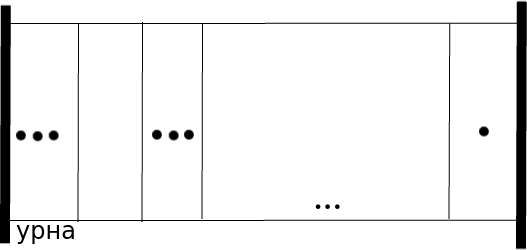
\includegraphics[width=.4\textwidth]{./pictures/1_10.png}
  \caption{Заполнение урн}
  \label{fig:110}
\end{figure}
\end{enumerate}

Урна находится между двумя палочками.
В одной урне может быть от $k_i$ шариков.
Точками обознычены шарики.
На данном рисунке в первой и третьей урнах находится по 3 шарика, во второй --- ни одного, в последней --- 1.

Палочек есть 19, а точечек (это конфеты) --- 20.
Их должны расставить на $19 + 20$ мест произвольным образом.
Количество этих решений является таким:
$$C_{20+20-1}^{19} \cdot C_{20}^{20} =
C_{39}^{19} =
\frac{39!}{19!20!} =
68923264410.$$

\subsubsection*{1.11}

\textit{Задание.} Вычислить количество неубывающих путей на двумерной целочисленной решётке
$$ \mathbb{Z}_+^2 = \{ \left( i, j \right): i, j = 0, 1, 2,  \dotsc \},$$
которые начинаются в точке $ \left( 0, 0 \right) $ и приводят в точку $ \left( m, n \right) $.
(Путь считается неубывающим, если на каждом шаге изменяется только одна координата, увеличиваясь на единицу.)

\textit{Решение.} Имеем пути, состоящие из $m+n$ ходов, среди которых ровно m <<горизонтальных>> и n <<вертикальных>> ходов.
Если выберем, на каких шагах увеличиваем одну координату (например, вертикальную), будем однозначно знать, где увеличиваем вторую координату (идём по горизонтали).
Значит, достаточно расставить m одинаковых шагов вверх на $n+m$ разных ячеек.
Это будет $$ C_{n+m}^m = \frac{ \left( n+m \right)!}{n!m!}.$$

\subsubsection*{1.12}

\textit{Задание.} Вычислить количество разных частных производных порядка r бесконечно дифференцируемой функции n переменных $f\left(x_1,  \dotsc , x_n\right)$.

\textit{Решение.} Функция бесконечно дифференцируема, значит, производная порядка r есть.
Рассмотрим функцию $f(x, y)$.
Производные первого порядка: $f'_x, f'_y$.
Первая производная --- одномерная матрица (вектор).
Производные второго порядка для
$f(x, y)$: $f''_{xx}, f''_{xy}, f''_{yx}, f''_{yy}$. $f''_{xy}$ и $f''_{yx}$
одинаковые.
Представим вторую производную в виде матрицы:
$$
\begin{pmatrix}
  xx & yx \\
  xy & yy \\ 
\end{pmatrix}
$$

Если три переменные:
$$
\begin{pmatrix}
  xx & yx & zx \\
  xy & yy & zy \\
  xz & yz & zz \\ 
\end{pmatrix}
$$

Строим матрицы по определённому алгоритму.
Столбцы --- это первое измерение, а строки --- второе.
Столбцы соответствуют x, y и z, и в ячейках столбцов на первой позиции стоит соответствующий дифференциал.
В ячейках строк указано, какой дифференциал будет вторым.

Рассмотрим третью производную для функции трёх переменных --- это трёхмерная матрица.
Третье измерение показывает, какой дифференциал будет третьим.
Значит, срез --- это то, где третьи дифференциалы фиксированы.
Получится три обычные матрицы: в первой на третьей позиции будут x, во второй --- y, а в третьей --- z.
Имеем: 
$$
\begin{pmatrix}
xxx & yxx & zxx \\ 
xyx & yyx & zyx \\
xzx & yzx & zzx \\
\end{pmatrix}
,
\begin{pmatrix}
xxy & yxy & zxy \\
xyy & yyy & zyy \\
xzy & yzy & zzy \\
\end{pmatrix}
,
\begin{pmatrix}
xxz & yxz & zxz \\
xyz & yyz & zyz \\
xzz & yzz & zzz \\
\end{pmatrix}
.$$

Матрицы записаны с учётом повторения элементов, значит нужно взять только те элементы, которые лежат на диагонали и с одной стороны от неё (треугольник).
Задача сведена к подсчёту количества элементов в r-мерной матрице $n\times n$.

Производный первого порядка есть столько же, сколько переменных у функции, т.е. n.

Найдём количество элементов двумерной матрицы $n\times n$, её верхнего треугольника.
Всего элементов в матрице $n\cdot n=n^2$.
Возьмём половину: $$\frac{n\cdot n}{2}$$ и прибавим ещё половину диагонали, чтобы получить треугольник, получаем
$$ \frac{n \cdot n}{2} + \frac{n}{2} = \frac{n(n+1)}{2}.$$

Для трёхмерной матрицы $n\times n$ проделываем аналогичные шаги.
Всего есть $n \cdot n \cdot n = n^3$ элементов, на диагонали --- $n \cdot n = n^2$ элементов.
Имеем: $$ \frac{n \cdot n \cdot n}{2} + \frac{n \cdot n}{2} = \frac{n^2(n+1)}{2}.$$

Обобщим для r-мерной матрицы.
Всего элементов $n^r$, элементов на диагонали $n^{r-1}$.
Отсюда имеем, что элементов на диагонали и выше её
$$ \frac{n^r}{2} + \frac{n^{r-1}}{2} = \frac{n^{r-1}(n+1)}{2}.$$

Это и есть число разных частных производных функции n переменных порядка r.

\subsubsection*{1.13}

\textit{Задание.} Пусть $\omega_m$ --- количество таких перестановок элементов множества $\{1, 2,  \dotsc , n\}$, что ни одно из чисел не остаётся на своём месте.
Доказать, что величина $ p_n = \frac{\omega_n}{n!}$ равна
$$ p_n = \frac{1}{2!} - \frac{1}{3!} + \dotsc + \frac{\left(-1\right)^n}{n!}.$$

\textit{Решение.} Найдём значение величины $\omega_n$.

Любая перестановка $k_1k_2 \dotsc k_n$ чисел $1, 2,  \dotsc , n$ означает вариант перестановки чисел, при котором i-е число стоит на $k_i$-м месте.
Например, в случае четырёх чисел перестановка 3241 означает,
что на первом месте стоит тройка $ \left( k_1 = 3 \right) $,
на втором --- двойка (на своём месте, $k_2=2$), на третьем --- четвёртая $ \left( k_3 = 4 \right) $ и на последнем --- первая $ \left( k_4 = 1 \right) $.
Наоборот, каждый вариант перестановки чисел обозначается единственной перестановкой чисел $1, 2,  \dotsc , n$.

Будем говорить, что в перестановки
$ k_1 k_2 \dotsc k_n $ чисел $1, 2,  \dotsc , n$
число i стоит на своём месте, если $ k_i = i $ (например, в перестановке 3241 двойка стоит на своём месте).
Нас интересует количество беспорядков, то есть таких перестановок, в которых ни одно из чисел не стоит на своём месте.
Число беспорядков можно найти, вычитая из общего количества перестановок, равного $n!$, количество тех перестановок, в которых хотя бы одно из чисел стоит на своём месте.

Пусть $A_i$ --- множество перестановок, в которых число i стоит на своём месте $\left(i=1, 2,  \dotsc , n\right)$.
Искомое число $\omega_n$ беспорядков, таким образом, равно
\begin{equation*}
\begin{split}
\omega_n =
n! - |A_1 \cup A_2 \cup \dotsc \cup A_n| = n! - \sum \limits_i |A_i| + \sum \limits_{i<j} |A_i \cap A_j| - \\
-\sum \limits_{i<j<k} |A_i \cap A_j \cap A_k| + \dotsc + \left( -1 \right)^n |A_1 \cap A_2 \cap \dotsc \cap A_n|.
\end{split}
\end{equation*}

$ |A_i| = \left( n-1 \right)!$, поэтому
$$ \sum \limits_i |A_i| = n \cdot \left( n-1 \right)! = n!.$$

Так же $ |A_i \cap A_j| = \left( n-2 \right)!$ и
$$ \sum \limits_{i<j} |A_i \cap A_j| = C_n^2 \cdot \left( n-2 \right)! = \frac{n \left( n-1 \right)}{2!} \cdot \left( n-2 \right)! = \frac{n!}{2!}.$$

Аналогично $ |A_i \cap A_j \cap A_k| = \left( n-3 \right)!$ и
$$ \sum \limits_{i<j<k} |A_i \cap A_j \cap A_k| =
C_n^3 \cdot \left( n-3 \right)! =
\frac{n \left( n-1 \right) \left( n-3 \right) }{3!} \cdot \left( n-3 \right)! =
\frac{n!}{3!}.$$

Теперь приходим к нужной формуле:
$$ \omega_n =
n! - n! + \frac{n!}{2!} =
\frac{n!}{3!} + \dotsc + \left( -1 \right)^n =
n! \cdot \sum \limits_{k=0}^n \frac{ \left( -1 \right)^k }{k!}.$$

Так как числа переставляются случайным образом, то вероятность беспорядка равна
$$ p_n =
\frac{ \omega_n }{n!} =
\frac{1}{n!} \left( \frac{n!}{2!} - \frac{n!}{3!} + \dotsc + \left( -1 \right)^n \right) =
\frac{1}{2!} - \frac{1}{3!} + \dotsc + \frac{ \left( -1 \right)^n}{n!}.$$

\subsubsection*{1.14}

\textit{Задание.} В классе учится 35 учеников.
Из них 20 занимаются в математическом кружке, 11 --- в физическом, а 10 учеников не посещают ни одного кружка.
Сколько учеников посещают математический и физический кружок.
Сколько учеников посещают только математический кружок?

\textit{Решение.} Изобразим диаграмму Эйлера-Венна для данной задачи на рисунке \ref{fig:114}. 

\begin{figure}[h!]
  \centering
  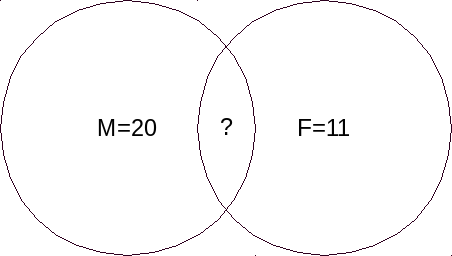
\includegraphics[width=.4\textwidth]{./pictures/1_14.png}
  \caption{Диаграмма Эйлера-Венна для задачи 1.14}
  \label{fig:114}
\end{figure}

Найдём, сколько учеников занимается хотя бы в одном кружке.
Это будет $35-10=25$ учеников.
Это есть количество элементов объединения двух множеств:
$$ |M \cup F| =
|M| + |F| - |M \cap F| =
25.$$
Отсюда можем найти, сколько учеников посещают и математический, и физический кружки:
$$ |M \cap F| =
|M| + |F| - |M \cup F| =
20 + 11 - 25 = 6.$$
Только математический кружок посещает $ |M| - |M \cap F| = 20 - 6 = 14$ учеников.

\addcontentsline{toc}{section}{Дополнительные задачи}
\section*{Дополнительные задачи}

\subsubsection*{1.15}

\textit{Задание.} Пусть множество X содержит n элементов, а множество Y --- m элементов.
Вычислить:
\begin{enumerate}[label=\alph*)]
\item количество функций из X в Y;
\item количество инъекций из X в Y $\left(n\leq m\right)$;
\item количество биекций из X в Y $\left(n=m\right)$.
\end{enumerate}

\textit{Решение.}
\begin{enumerate}[label=\alph*)]
\item Можно считать, что $ X = \{1,  \dotsc , n \}, Y = \{1,  \dotsc , m \}$.
Каждую функцию можно отождествлять с последовательностью $ < f(1),  \dotsc , f(n) ) > = < y_1,  \dotsc , y_n > $.
Каждый член $y_i$ последовательности можно выбрать m способами, что даёт $m^n$ возможностей выбора $ < y_1,  \dotsc , y_n > $.

\item Будем определять число инъективных (то есть имеющих все различные члены) последовательностей $ < y_1,  \dotsc , y_n > $.
Элемент $y_1$ может быть выбран m способами, элемент $y_2$ можно выбрать $m-1$ способом из оставшихся элементов.
Если уже выбраны элементы $ y_1,  \dotsc , y_{i-1} $,
то в качестве $y_i$ может быть выбран любой из $m-i+1$ элементов множества
$Y\setminus\{y_1,  \dotsc , y_{i-1}\}$. Принимаем, что $ m \geq n $. если $ n > m $,
то искомое число функций равно 0.
Это даёт
$$m\left(m-1\right) \dotsc (m+n-1)
=\frac{m!}{\left(m-n\right)!}$$
возможность выбора инъективных последовательностей $<y_1,  \dotsc , y_n>$.

\item Если $n=m$, то любое инъективное отображение будет биективным.
Число всех биективных отражений X в Y равно $n!$ при $m = n$ и 0 при $m \neq n$.
\end{enumerate}

\addcontentsline{toc}{section}{Домашнее задание}
\section*{Домашнее задание}

\subsubsection*{1.16}

\textit{Задание.} Подсчитать, сколько трёхзначных чисел можно записать с помощью:
\begin{enumerate}[label=\alph*)]
\item цифр 0, 1, 2, 3, 4, 5;
\item цифр 0, 1, 2, 3, 4, 5, если каждую из цифр использовать не больше одного раза.
\end{enumerate}

\textit{Решение.} Трёхзначное число можно рассматривать как трёхмерный вектор.
Первой компонентой этого вектора может быть любая цифра из множества
$$ A_1 = \{ 1, 2, 3, 4, 5 \} $$
(запись числа не может начинаться с 0).

\begin{enumerate}[label=\alph*)]
\item На остальных позициях может стоять любая цифра, то есть
$$ A_i = \{ 0, 1, 2, 3, 4, 5 \}, i = 2, 3.$$
Отсюда имеем, что из указанных цифр можно составить $ 5 \cdot 6 \cdot 6 = 180$ трёхзначных чисел.

\item На остальных позициях могут стоять любые цифры (кроме тех, что стояли на предыдущих позициях).
Отсюда имеем, что из указанных цифр можно составить $ 5 \cdot 5 \cdot 4 = 100 $ трёхзначных чисел.
\end{enumerate}

\subsubsection*{1.17}

\textit{Задание.} Подсчитать количество пятизначных чисел, которые делятся на 5.

\textit{Решение.} Пятизначное число можно рассматривать как пятимерный вектор.
Первой компонентой этого вектора может быть любая цифра из множества
$$ A_1 = \{ 1, 2, 3, 4, 5, 6, 7, 8, 9 \} $$
(запись числа не может начинаться с 0), а на остальных позициях (кроме последней) может стоять любая цифра, то есть
$$ A_i = \{ 0, 1, 2, 3, 4, 5, 6, 7, 8, 9 \}, i = 2, 3, 4.$$
На последней позиции может стоять цифра из множества $ A_5 = \{ 0, 5 \}$ (чтобы число делилось на 5, оно должно оканчиваться на 0 или 5).
Отсюда имеем, что можно составить $ 9 \cdot 10 \cdot 10 \cdot 10 \cdot 2 = 18000$ пятизначных чисел, которые делятся на 5.

\subsubsection*{1.18}

\textit{Задание.} Замок компьютерного центра состоит из пяти кнопок, пронумерованных от 1 до 5.
Чтобы открыть замок, необходимо первые две определённые кнопки нажать одновременно, а потом одну за другой нажать другие три кнопки в определённой последовательности. Подсчитать количество способов закодировать вход в компьютерный центр.

\textit{Решение.} Рассмотрим 3 случая: 
\begin{enumerate}[label=\alph*)]
\item сначала необходимо нажать две разные кнопки, далее их отпускают, и все остальные кнопки могут быть любыми; 
\item первые две кнопки держатся нажатыми, следующие кнопки не могут быть такими, как первые две; 
\item нельзя нажать одну и ту же кнопку больше одного раза (кнопки остаются нажатыми).
\end{enumerate}

Количество способов нажать первые две кнопки равна количеству двухэлементных подмножеств в множестве из пяти элементов, то есть
$$ C_5^2 = \frac{5!}{2! \left( 5 - 2 \right)!} = 10.$$

В случае а) количество способов закодировать вход в компьютерный центр равно
$$ C_5^2 \cdot 5^3 = 1250.$$
Общая формула: $ C_N^n \cdot N^m $, где N --- количество кнопок, n кнопок нажимаются вместе, а затем m кнопок --- по очереди.

В случае б) после нажатия двух кнопок, остаётся только 3 кнопки, которые необходимо нажать в правильном порядке,
поэтому количество способов по предыдущей формуле равно
$$ C_5^2 \cdot 3^3 = 270.$$

В случае в) все кнопки должны быть нажаты один раз, поэтому количество способов закодировать вход равно
$$ C_5^2 \cdot 3 \cdot 2 \cdot 1 = 60.$$

\subsubsection*{1.19}

\textit{Задание.} Колоду игральных карт (52 карты, 4 масти по 13 карт в каждой) тщательно перетасовали.
Подсчитать количество способов выбрать из неё 6 карт без возвращения так, чтобы среди них:
\begin{enumerate}[label=\alph*)]
\item был пиковый король;
\item были представители всех мастей;
\item было ровно 5 карт одной масти.
\end{enumerate}

\textit{Решение.}
\begin{enumerate}[label=\alph*)]
\item Выбрать пикового короля есть только один способ.
Остальные 6 карт могут быть любыми из оставшихся 51 карты.
Выбрать эти 5 карт можно $ C_{51}^5 $ способами.
Отсюда имеем, что из колоды можно выбрать 6 карт, среди которых был бы пиковый король, $ 1 \cdot C_{51}^5 $ числом способов.

\item Сначала выберем по одной карте каждой масти.
Количество способов выбрать одну карту определённой масти равно $C_{13}^1$, так как имеется 13 карт каждой масти.
Так как всего есть 4 масти, то нужно выбрать 4 карты (по одной карте каждой масти).
Тогда количество способов выбрать 4 карты разных мастей равно
$$ C_{13}^1 \cdot C_{13}^1 \cdot C_{13}^1 \cdot C_{13}^1 =
\left( C_{13}^1 \right)^4.$$
Остаётся выбрать две произвольные карты из оставшихся.
После выбора четырёх карт разных мастей в колоде осталось $ 52 - 4 = 48 $ карт.
Число способов выбрать из них две карты равно $ C_{48}^2 $.
Отсюда имеем, что количество способов выбрать из данной колоды 6 карт без возвращения таким образом, чтобы среди них были представители всех мастей, равно
$$ \left( C_{13}^1 \right) \cdot C_{48}^2.$$

\item Сначала нужно выбрать 5 карт одной масти.
В одной масти 13 карт, следовательно число способов выбрать 5 карт одной масти равно $ C_{13}^5 $.
Так как всего мастей 4, и нам не важно, какой именно масти будут 5 вытянутых карт (главное, чтобы одной), то число способов будет равно
$$ 4 \cdot C_{13}^5.$$
Шестая карта должна быть любой, но отличатся с предыдущими пятью мастью, то есть её можно выбрать из $ 52 - 13 = 39 $ карт.
Число способов это сделать равно $ C_{39}^1 $.
Отсюда имеем, что число способов выбрать из колоды карт 6 карт так, чтобы среди них было ровно 5 карт одной масти, равно
$$ 4 \cdot C_{13}^5 \cdot C_{39}^1.$$
\end{enumerate}

\subsubsection*{1.20}

\textit{Задание.} Сколькими способами можно разместить 10 одинаковых открыток в 4 почтовых ящиках так, чтобы:
\begin{enumerate}[label=\alph*)]
\item не было пустых ящиков;
\item во втором ящике было 3 открытки.
\end{enumerate}

\textit{Решение.}
\begin{enumerate}[label=\alph*)]
\item Рассмотрим случай, когда в каждый ящик должна быть помещена хотя бы одна открытка.
Используем метод перегородок.
Выложим открытки в ряд.
Для определения расклада открыток по четырём почтовым ящикам разделим ряд тремя перегородками на 4 группы:
первая группа для первого ящика, вторая --- для второго и так далее.
Таким образом, число вариантов раскладки открыток по ящикам равно числу способов разложения трёх перегородок.
Перегородки могут стоять на любом из 9 мест (между 10 открытками --- 9 промежутков).
Поэтому число возможных расположений равно $ C_9^3 $.

\item Рассмотрим случай, когда во второй ящик должны быть помещены 3 открытки.
Поскольку открытки одинаковые, то во второй ящик можно сразу положить 3 открытки.
В этом случае нужно распределить $ 10 - 3 = 7$ одинаковых открыток между тремя почтовыми ящиками.

Используем метод перегородок.
Рассмотрим ряд из 9 предметов: 7 одинаковых открыток и 2 одинаковые перегородки, расположенных в произвольном порядке.
Каждый такой ряд однозначно соответствует некоторому способу раскладки открыток по ящикам:
в первый ящик попадают открытки, расположенные левее первой перегородки,
во второй --- расположенные между первой и второй перегородками и т.д. (между какими-то перегородками открыток может и не быть).
Поэтому число способов раскладки открыток по ящикам равно числу различных рядов из 7 открыток и 2 перегородок,
т.е равно $ C_9^2 $ (ряд определяется теми двумя местами из 9, на которых стоят перегородки).
\end{enumerate}

\subsubsection*{1.21}

\textit{Задание.} Сколькими способами можно распределить 10 путёвок среди 10 студентов (по одной каждому), если:
\begin{enumerate}[label=\alph*)]
\item все путёвки разные;
\item есть 4 путёвки одного типа и 6 --- другого?
\end{enumerate}

\textit{Решение.}
\begin{enumerate}[label=\alph*)]
\item Количество возможных перестановок 10 разных путёвок равно $10!$;

\item если будем считать все 10 элементов перестановки с повторениями различными, то всего различных вариантов перестановок 10 путёвок ---
$$ ( 4 + 6 )! = 10!.$$
Однако среди этих перестановок не все различны.
Все путёвки одного типа можно переставлять местами друг с другом, и от этого перестановка не изменится.
Точно так же, можем переставлять путёвки другого типа.
Таким образом, перестановка может быть записана $4!6!$ способами.
Следовательно, число различных перестановок с повторениями равно
$$ \frac{ ( 4 + 6 )! }{ 4!6! } = \frac{10!}{4!6!}.$$
\end{enumerate}

\subsubsection*{1.22}

\textit{Задание.} Доказать, что количество неубывающих путей на r-мерной целочисленной решётке
$$ \mathbb{Z}_+^r = \{ \left( i_1,  \dotsc , i_r \right) : i_1,  \dotsc , i_r = 0, 1, 2,  \dotsc \} ,$$
которые начинаются в точке $ \left( 0,  \dotsc , 0 \right) $ и приводят в точку $ \left( n_1,  \dotsc , n_r \right) $, равно
$$ C_N \left( n_1,  \dotsc , n_r \right) =
\frac{N!}{n_1! \dotsc n_r!},$$
где $ N = \sum \limits_{ i = 1 }^r n_i$.
(Путь считается неубывающим, если на каждом шаге изменяется только одна координата, увеличиваясь на единицу.)

\textit{Решение.} Имеем пути, состоящие из $ n_1 + \dotsc + n_r$ ходов,
среди которых ровно $n_1$ ходов в направлении $ r_1$,  $\dotsc$ , и $n_r$ ходов в направлении $r_n$.
Если выберем, на каких шагах увеличиваем первую координату, будем знать, где увеличиваем остальные координаты.
Далее выберем, на каких шагах увеличиваем вторую координату.
И так необходимо определить, где увеличиваем $ n_1+ \dotsc n_{r-1}$ координат.
Тогда будем однозначно знать, где увеличиваем последнюю координату.
Это будет
$$ \frac{ \left( n_1 + \dotsc + n_r \right) }{ n_1! \dotsc n_r! }.$$

\subsubsection*{1.23}

\textit{Задание.} Из 100 студентов английский язык знают 28,
немецкий --- 30, французский --- 42, английский и немецкий --- 8, английский и французский --- 10, немецкий и французский --- 5, а все три языка знают 3 студента.
Сколько студентов не знают ни одного языка?

\textit{Решение.} Условие задачи представлено на рисунке \ref{fig:123} в виде диаграммы Эйлера-Венна. 

\begin{figure}[h!]
  \centering
  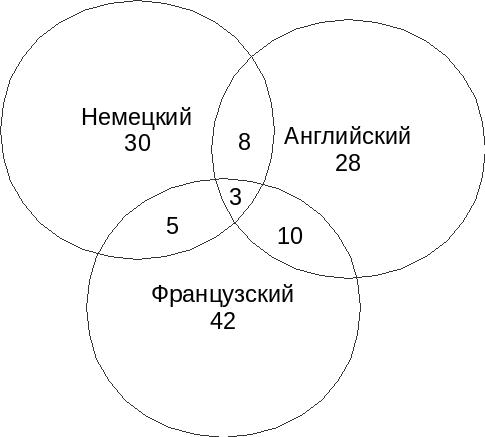
\includegraphics[width=.4\textwidth]{./pictures/1_23.png}
  \caption{Диаграмма Эйлера-Венна для задачи 1.23}
  \label{fig:123}
\end{figure}

Сначала найдём, сколько студентов знает хотя бы один язык.
Это есть мощность (количество элементов) объединения трёх множеств: Английский, Немецкий и Французский, которые обозначим первыми буквами.
Мощность объединения трёх множеств можно найти как сумму мощностей этих множеств, но, так как они пересекаются,
необходимо отнять мощности их пересечений и добавить пересечение всех трёх множеств, потому что его отняли дважды.
Имеем
\begin{equation*}
\begin{split}
|H \cup A \cup F| =
|H| + |A| + |F| - |H \cap A| - |A \cap F| - |H \cap F| + |H \cap A \cap F| = \\
= 30 + 42 + 28 - 5 - 8 - 10 + 3 = 80.
\end{split}
\end{equation*}

Все остальные студенты из ста не знают ни одного языка.
Их 
$$ 100 - 80 = 20.$$

\addcontentsline{toc}{chapter}{Занятие 2. События и операции над ними. Пространство элементарных событий}
\chapter*{Занятие 2. События и операции над ними. Пространство элементарных событий}

\addcontentsline{toc}{section}{Контрольные вопросы и задания}
\section*{Контрольные вопросы и задания}

\subsubsection*{Приведите определение вероятностного эксперимента, вероятностного пространства, случайного события.}

Вероятностным экспериментом называется явление, исход которого для нас не определён, и которое можно повторить любое число раз независимым образом.

Вероятностное пространство --- совокупность всех исходов вероятностного эксперимента, $ \Omega $.

Случайное событие --- подмножество всех исходов вероятностного эксперимента, $ A \subset \Omega $.

\subsubsection*{Запишите основные операции над случайными событиями и дайте их теоретико-множественную интерпретацию.}

Операции будем иллюстрировать на диаграммах Эйлера-Венна.
На рис.\ref{fig:2} заштрихованы области, которые соответствуют событиям, являющимся результатами таких операций.

Пересечением (произведением) двух событий А и В называют событие С, происходящее тогда и только тогда,
когда одновременно происходят оба события А и В, т.е событие,
состоящее из тех и только тех элементарных исходов, которые принадлежат и события А, и событию В (рис.\ref{fig:2}, а).

Пересечение событий А и В записывают следующим образом: $ C = A \cap B $, или $ C = AB $.

События А и В называют несовместимыми, или непересекающимися, если их пересечение является невозможным событием, т.е если $ A \cap B = \emptyset$ (рис.\ref{fig:2}, б).

В противном случае события называют совместимыми, или пересекающимися.

\begin{figure}[h!]
  \centering
  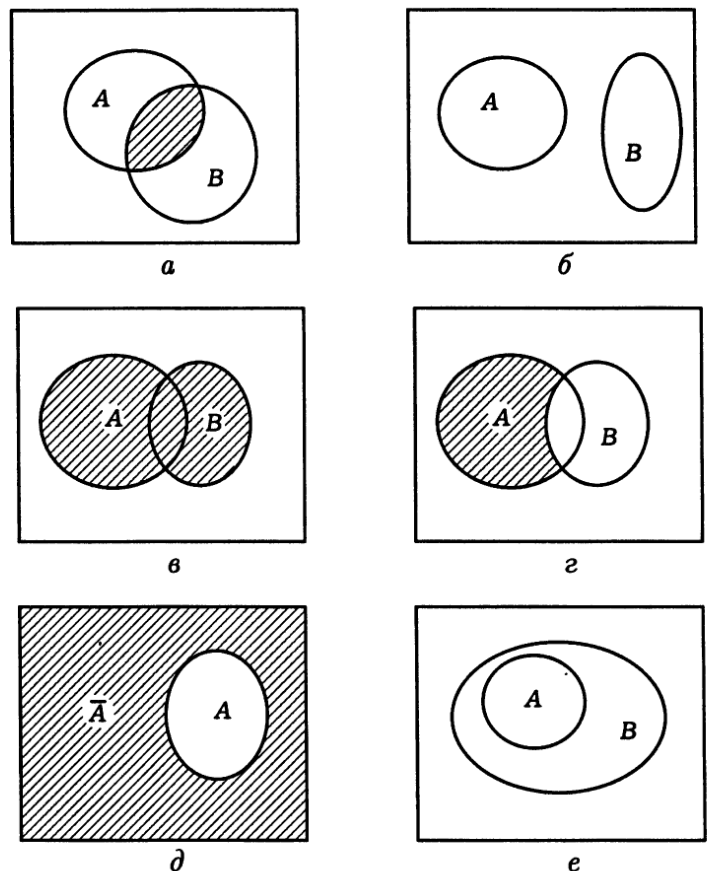
\includegraphics[width=.7\textwidth]{./pictures/2.png}
  \caption{Диаграммы Эйлера-Венна для операций над событиями}
  \label{fig:2}
\end{figure}

Объединением (суммой) двух событий А и В называют событие С,
происходящее тогда и только тогда,
когда происходит хотя бы одно из событий А или В, т.е.
событие С, состоящее из тех элементарных исходов, которые принадлежат хотя бы одному из подмножеств А или В (рис.\ref{fig:2}, в).

Объединение событий А и В записывают в виде $ C = A \cup B $.

Разностью двух событий А и В называют событие С,
происходящее тогда и только тогда,
когда происходит событие А,
но не происходит событие В, т.е. событие С, состоящее из тех элементарных исходов, которые принадлежат А, но не принадлежат В (рис.\ref{fig:2}, г).

Разность событий А и В записывают в виде: $ C = A \setminus B $.

Дополнением события А (обычно обозначают $ \overline{A} $) называют событие, происходящее тогда и только тогда, когда не происходит событие А (рис.\ref{fig:2}, д).
Другими словами, $ \overline{A} = \Omega \setminus A $.

Событие А включено в событие В,
что записывается $ A \subset B $,
если появление события А обязательно влечёт за собой наступление события В (рис.\ref{fig:2}, е),
или каждый элементарный исход $ \omega $, принадлежащий А, обязательно принадлежит и событию В.

Верхний предел последовательности $ \{ A_n : n \geq 1 \} $ --- это случайное событие,
состоящее в том, что произошло бесконечно много событий из исходной последовательности:
$$ \varlimsup \limits_{ n \to \infty } A_n =
\bigcap \limits_{n \geq 1} \bigcup \limits_{ m \geq n } A_m.$$

$ \forall n \exists m \geq n : A_m $ произошло.

Нижний предел последовательности:
$ \{ A_n : n \geq 1 \} $ --- это случайное событие, состоящее в том, что произошли все события, начиная с некоторого из исходной последовательности:
$$ \varliminf \limits_{ n \to \infty } A_n =
\bigcup \limits_{ n = 1 }^\infty \bigcap \limits_{ m = n }^\infty A_m.$$

$ \exists n \forall m \geq n $ происходит событие $A_m$.

\subsubsection*{Сформулируйте законы де Моргана.}

Первый закон де Моргана гласит: <<Если неверно, что есть и первое, и второе, то неверно либо одно из, либо оба>>, что выражается следующей формулой:
$ \overline{ AB } = \overline{ A } \cup \overline{ B }$.

Второй закон де Моргана гласит: <<Если неверно, что есть первое, или неверно, что есть второе, то неверно, что есть первое и второе>>, что выражается следующей формулой:
$ \overline{ A \cup B} = \overline{ A }$ $ \overline{ B }$.

Законы де Моргана верны для любого конечного числа событий:
\begin{equation*}
\begin{split}
\overline{ A_1 \cup A_2 \cup \dotsc \cup A_n } =
\overline{ A_1 } \, \overline{ A_2 } \, \dotsc \overline{ A_n }, \\
\overline{ A_1 A_2 \dotsc A_n } =
\overline{ A_1 } \cup \overline{ A_2 } \cup \dotsc \cup \overline{ A_n }.
\end{split}
\end{equation*}

\addcontentsline{toc}{section}{Аудиторные задачи}
\section*{Аудиторные задачи}

\subsubsection*{2.3}

\textit{Задание.} Рассмотрим эксперимент, который состоит в подбрасывании трёх монет.
Постройте множество $ \Omega $ элементарных событий этого эксперимента.
Опишите событие A, которое состоит в том, что выпало не меньше двух гербов.
Вычислите вероятность события A.

\textit{Решение.} Пусть эксперимент состоит в подбрасывании одной монеты.
При математическом описании этого опыта естественно отвлечься от несущественных возможностей
(например, монета встанет на ребро) и ограничиться только двумя элементарными исходами:
выпадение <<герба>> (обозначим этот исход $ \omega_1 $) и выпадением <<цифры>> (обозначим этот исход $\omega_2$).
Таким образом, $ \Omega_1 = \{ \omega_1, \omega_2 \} $.

При подбрасывании двух монет пространство элементарных исходов будет содержать три элемента,
т.е. $ \Omega_2 = \{ \omega_{11}, \omega_{12}, \omega_{22} \} $, где, например, $\omega_{11}$ --- появление <<герба>> и на первой, и на второй монете.

При подбрасывании трёх монет пространство элементарных исходов будет содержать элементов, т.е.
$ \Omega_3 = \Omega = \{ \omega_{111}, \omega_{112}, \omega_{122}, \omega_{222} \} $, где, например,
$ \omega_{111} $ --- появление <<герба>> и на первой, и на второй, и на третьей монете.

Событие A состоит в том, что выпало не меньше двух гербов, т.е. два или три герба.
Выберем из $ \Omega $ такие исходы: $ A = \{ \omega_{122}, \omega_{222} \} $.

Поскольку $ |A| = 2, | \Omega | = 4$, то
$$ P(A) = \frac{ |A| }{| \Omega |} =
\frac{2}{4} =
\frac{1}{2}.$$

\subsubsection*{2.4}

\textit{Задание.} Пусть A, B, C --- произвольные события.
Найдите выражения для событий, который состоят в том, что из событий A, B и C:
\begin{enumerate}[label=\alph*)]
\item произошло только  A;
\item произошли A и B, но не произошло C;
\item произошли все три события;
\item произошло хотя бы одно из этих событий;
\item произошло хотя бы два события;
\item произошло одно и только одно событие;
\item произошло два и только два события;
\item ни одно из событий не произошло;
\item произошло не больше двух событий.
\end{enumerate}

\textit{Решение.}
\begin{enumerate}[label=\alph*)]
\item $ A \cap \overline{ B } \cap \overline{ C } $;
\item $ A \cap B \cap \overline{ C } $;
\item $ A \cap B \cap C $;
\item $ A \cup B \cup C $;
\item $ \left( A \cap B  \cap \overline{C} \right) \cup \left( A \cap \overline{B} \cap C \right) \cup \left( \overline{A} \cap B \cap C \right) $;
\item $ \left( A \cap \overline{ B } \cap \overline{ C } \right) \cup \left( B \cap \overline{ A } \cap \overline{ C } \right)
\cup \left( C \cap \overline{ A } \cap \overline{ B } \right) $;
\item $ \left( A \cap B \cap \overline{ C } \right) \cup \left( A \cap C \cap \overline{ B } \right) \cup \left( B \cap C \cap \overline{ A } \right) $;
\item $ \overline{ A } \cap \overline{ B } \cap \overline{ C } $;
\item $ \left( \overline{ A } \cap \overline{ B } \cap \overline{ C } \right) \cup
\left( A \cap \overline{ B } \cap \overline{ C } \right) \cup
\left( B \cap \overline{ A } \cap \overline{ C } \right) \cup
\left( C \cap \overline{ A } \cap \overline{ B } \right) \cup
\left( A \cap B \cap \overline{ C } \right) \cup \\
\cup \left( A \cap C \cap \overline{ B } \right) \cup
\left( B \cap C \cap \overline{ A } \right)$.
\end{enumerate}

\subsubsection*{2.5}

\textit{Задание.} Пусть A и B --- некоторые события.
Упростите выражение
$$ C = \overline{ \overline{ A \cap \overline{ B } } \cup \overline{ A \cup B } \cup \left( B \cap A \right) }.$$

\textit{Решение.}
$ C =
\overline{ \overline{ A \cap \overline{ B }}} \cap \overline{ \overline{ A \cup B }} \cap \overline{ B \cap A } =
A \cap \overline{B} \cap \left( A \cup B \right) \cap \left( \overline{B} \cup \overline{A} \right) = \\
= A \cap \left[ \left( \overline{B} \cap A \right) \cup \left( \overline{B} \cap B \right) \right] \cap \left( \overline{B} \cup \overline{A} \right) =
A \cap \overline{B} \cap A \cap \left( \overline{B} \cup \overline{A} \right) =
A \cap \overline{B} \cap \left( \overline{B} \cup \overline{A} \right) = \\
= \left[ \left( A \cap \overline{B} \right) \cup \left( A \cap \overline{A} \right) \right] \cap \overline{B} =
A \cap \overline{B} \cap \overline{B} =
A \cap \overline{B}$.

\subsubsection*{2.6}

\textit{Задание.} Пусть $ \{ A_n, n \in \mathbb{N} \}, \{ B_n, n \in \mathbb{N} \} $ --- некоторые последовательности событий.
Объясните, что значат события $ \varlimsup \limits_{n \to \infty } A_n, \varliminf \limits_{n \to \infty } A_n$.
Докажите, что:
\begin{enumerate}[label=\alph*)]
\item $ \overline{ \varlimsup \limits_{ n \to \infty } A_n } =
\varliminf \limits_{ n \to \infty } \overline{ A_n }$;
\item $ \varlimsup \limits_{ n \to \infty } \left( A_n \cup B_n \right) =
\varlimsup \limits_{ n \to \infty } A_n \cup \varlimsup \limits_{ n \to \infty } B_n $.
\end{enumerate}

\textit{Решение.} Верхний предел последовательности $ \{ A_n : n \geq 1 \} $ ---
это случайное событие, состоящее в том, что произошло бесконечно много событий из исходной последовательности:
$$ \varlimsup \limits_{ n \to \infty } A_n =
\bigcap \limits_{ n \geq 1 } \bigcup \limits_{ m \geq n} A_m.$$

$ \forall n \exists m \geq n : A_m $ произошло.

Нижний предел последовательности:
$ \{ A_n : n \geq 1 \}$ --- это случайное событие, состоящее в том, что произошли все события, начиная с некоторого из исходной последовательности:
$$ \varliminf \limits_{ n \to \infty } A_n =
\bigcup \limits_{ n = 1 }^\infty \bigcap \limits_{ m = n }^\infty A_m.$$

$ \exists n \forall m \geq n $ происходит событие $A_m$.

\begin{enumerate}[label=\alph*)]
\item $\overline{ \varlimsup \limits_{ n \to \infty } A_n } =
\overline{ \bigcap \limits_{ n \geq 1} \bigcup \limits_{ m \geq n} A_m } =
\bigcup \limits_{ n \geq 1} \overline{ \bigcup \limits_{ m \geq n} A_m } =
\bigcup \limits_{ n \geq 1} \bigcap \limits_{ m \geq n} \overline{ A_m } =
\varliminf \limits_{ n \to \infty} \overline{ A_n }$;

\item $\varlimsup \limits_{ n \to \infty } \left( A_n \cup B_n \right) =
\bigcap \limits_{ n \geq 1} \bigcup \limits_{ m \geq n} \left( A_m \cup B_m \right) =
\prod \limits_{ n = 1 }^\infty \sum \limits_{ m = n }^\infty \left( A_m + B_m \right) = \\
= \prod \limits_{ n = 1 }^\infty \sum \limits_{ m = n }^\infty A_m + \prod \limits_{ n = 1 }^\infty \sum \limits_{ m = n }^\infty B_m =
\varlimsup \limits_{ n \to \infty } A_n \cup \varlimsup \limits_{ n \to \infty } B_n $.
\end{enumerate}

\subsubsection*{2.7}

\textit{Задание.} Пусть $ \{ A_n, n \in \mathbb{N} \} $ --- некоторая последовательность событий, $ \mathbbm{1} ( A ) $ --- индикатор события A.
Докажите, что $ \mathbbm{ 1 } \left( \varlimsup \limits_{ n \to \infty } A_n \right) =
\varlimsup \limits_{ n \to \infty } \mathbbm{ 1 } \left( A_n \right) $.

\textit{Решение.} Рассмотрим 4 случая: 

\begin{enumerate}
\item $ \mathbbm{ 1 } \left( \varlimsup \limits_{ n \to \infty } A_n \right) = 0,
\varlimsup \limits_{ n \to \infty } \mathbbm{ 1 } \left( A_n \right) = 0 $;
\item $ \mathbbm{ 1 } \left( \varlimsup \limits_{ n \to \infty } A_n \right) = 0,
\varlimsup \limits_{ n \to \infty } \mathbbm{ 1 } \left( A_n \right) = 1 $;
\item $ \mathbbm{ 1 } \left( \varlimsup \limits_{ n \to \infty } A_n \right) = 1,
\varlimsup \limits_{ n \to \infty } \mathbbm{ 1 } \left( A_n \right) = 0 $;
\item $ \mathbbm{ 1 } \left( \varlimsup \limits_{ n \to \infty } A_n \right) = 1,
\varlimsup \limits_{ n \to \infty } \mathbbm{ 1 } \left( A_n \right) = 1 $.
\end{enumerate}

Нужно доказать, что возможны только первый и последний случаи.

Верхний предел последовательности
$ \{ A_n : n \geq 1 \} $ --- это случайное событие, состоящее в том, что произошло бесконечно много событий из исходной последовательности:
$$ \varlimsup \limits_{ n \to \infty } A_n =
\bigcap \limits_{ n \geq 1} \bigcup \limits_{ m \geq n} A_m.$$

Индикатор --- функция двух переменных:
$ \mathbbm{1} \left( \omega, A \right) $,
где $\omega$ --- элементарный исход (то, что произошло), A --- случайное событие (то, что рассматриваем).
Если $\omega \in A$, то индикатор равен 1, иначе --- 0.

Индикатор верхнего предела равен нулю
$ \left( \mathbbm{ 1 } \left( \varlimsup \limits_{ n \to \infty } A_n \right) = 0 \right)$ --- значит, произошло конечное множество событий из $A_n$.
Значит, с какого-то момента события перестали происходить, и предел индикаторов равен нулю: $ \varlimsup \limits_{ n \to \infty } \mathbbm{ 1 } \left( A_n \right) = 0$.

Если индикатор от верхнего предела равен единице
$$ \left( \mathbbm{ 1 } \left( \varlimsup \limits_{ n \to \infty } A_n \right) =
\mathbbm{ 1 } \left( \bigcap \limits_{ n \geq 1} \bigcup \limits_{ m \geq n } A_m \right) =
1 \right) ,$$
то произошло бесконечное множество событий из $A_n$.
Это значит, во-первых, что пересечение не пустое, а во-вторых, что элементарный исход принадлежит этому пересечению.
Верхний предел последовательности событий --- это такое случайное событие,
что каждый случайный исход из него принадлежит бесконечному количеству событий из последовательности.
Поэтому
$ \varlimsup \limits_{ n \to \infty } \mathbbm{ 1 } \left( A_n \right) = 1 $.

\subsubsection*{2.8}

\textit{Задание.} Пусть B и C --- два события.
Положим $ A_n = B $, если n чётное и $ A_n = C $, если n нечётное.
Найдите событие, которое состоит в том, что:
\begin{enumerate}[label=\alph*)]
\item произошло бесконечно много событий из последовательности $ \{ A_n \}_{ n = 1 }^\infty $;
\item произошло только конечное количество событий из последовательности $ \{ A_n \}_{ n = 1 }^\infty $.
\end{enumerate}

\textit{Решение.}
\begin{enumerate}[label=\alph*)]
\item По определению
$$ \varlimsup \limits_{ n \to \infty } A_n =
\bigcap \limits_{ n \geq 1} \bigcup \limits_{ m \geq n} A_m.$$

При $ n = 1: \bigcup \limits_{ m \geq 1} A_m = A_1 \cup A_2 \cup A_3 \cup \dotsc = B \cup C $.
Пересечение бесконечного количества одинаковых множеств даёт $ \varlimsup \limits_{ n \to \infty } A_n = B \cup C $;

\item это противоположное событие к тому, что произошло бесконечное количество событий из последовательности
$$ \overline{ \varlimsup \limits_{ n \to \infty } A_n} =
\overline{\bigcap \limits_{ n \geq 1} \bigcup \limits_{ m \geq n} A_m} =
\overline{B \cup C} =
\overline{B} \cap \overline{C}.$$
\end{enumerate}

\subsubsection*{2.9}

\textit{Задание.} Рассмотрим эксперимент, который состоит в выборе наугад точки в квадрате с вершинами в точках $ A(0, 0), B(0, 1), C(1, 1) $ и $ D(1, 0) $.
Опишите и изобразите вероятностное пространство этого эксперимента и следующие события:
\begin{enumerate}[label=\alph*)]
\item A = {данная точка оказалась на расстоянии не меньшем чем 1/4 от сторон квадрата};
\item B = {данная точка оказалась внутри круга с центром в начале координат и радиусом 1/2};
\item $ \overline{ A }, \overline{ B }, A \cap B $.
\end{enumerate}

\textit{Решение.} Пространство элементарных событий ( \ref{fig:29}, а)) опишем как множество упорядоченных пар
$ \Omega = \{ (x, y), 0 \leq x \geq 1, 0 \leq y \geq 1 \} $, где x --- первая координата точки, y --- вторая координата точки.

\begin{figure}[h!]
  \centering
  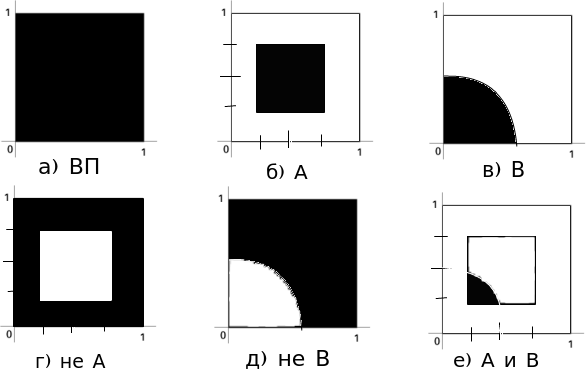
\includegraphics[width=.7\textwidth]{./pictures/2_9.png}
  \caption{Вероятностное пространство и события из задачи 2.9}
  \label{fig:29}
\end{figure}

\begin{enumerate}[label=\alph*)]
\item $ A = \{ (x, y), \frac{3}{4} \leq x \geq \frac{1}{4}, \frac{3}{4} \leq y \geq \frac{1}{4}, \} $ ( \ref{fig:29}, б));

\item $ B = \{ (x, y), x \geq 0, y \geq 0, x^2 + y^2 \leq \frac{1}{2} \} $ ( \ref{fig:29}, в));

\item событие $ \overline{ A } $ означает, что событие A не произошло, то есть расстояние от точки до сторон квадрата оказалось больше 1/4 ( \ref{fig:29}, г)):
$$ \overline{ A } =
\{ (x, y), \frac{3}{4} > x > \frac{1}{4},
\frac{3}{4} > y > \frac{1}{4} \}.$$

Событие $ \overline{ B } $ означает, что данная точка не оказалась внутри круга с центром в начале координат и радиусом 1/2 ( \ref{fig:29}, д)):
$$ \overline{ B } =
\{ (x, y),
\frac{1}{2} > x^2 + y^2 \leq 1,
x \leq 1,
y \leq 1. \} $$

Событие $ A \cap B $ означает, что произошло и событие A, и событие B ( \ref{fig:29}, е)).
Отсюда имеем, что данная точка оказалась на расстоянии не меньшем чем 1/4 от сторон квадрата, а так же внутри круга с центром в начале координат и радиусом 1/2, т.е.
$$ A \cap B =
\{ (x, y),
x \geq \frac{1}{4},
y \geq \frac{1}{4},
x^2 + y^2 \leq \frac{1}{2} \}.$$
\end{enumerate}

\addcontentsline{toc}{section}{Дополнительные задачи}
\section*{Дополнительные задачи}

\subsubsection*{2.10}

\textit{Задание.} Пусть A --- множество из n элементов,
$ A_1,  \dotsc , A_k $ --- подмножества A такие, что ни одно из подмножеств не является частью другого,
а $ i_1,  \dotsc , i_k $ --- количество элементов подмножеств $ A_1,  \dotsc , A_k $ соответственно.
Докажите, что
$$ \sum \limits_{ r = 1 }^k \frac{ 1 }{ C_n^{ i_r } } \leq 1.$$

\textit{Решение.} Умножим слева и справа на произведение знаменателей:
$$ \prod \limits_{r=1}^k C_n^{i_r} \sum \limits_{r=1}^k \frac{1}{C_n^{i_r}} \leq
\prod \limits_{r=1}^k C_n^{i_r}. $$

Внесём произведение под знак суммы:
$$ \sum \limits_{r=1}^k \frac{ \prod \limits_{r'=1}^k C_n^{i_{r'}}}{C_n^{i_r}} \leq
\prod \limits_{r=1}^k C_n^{i_r}. $$

Упростим:
$$ \sum \limits_{r=1}^k \prod \limits_{1 \leq r' \leq k}^{r' \neq r} C_n^{i_{r'}} \leq
\prod \limits_{r=1}^k C_n^{i_r}. $$

Обозначим номер наибольшего слагаемого как r:
$$r =
arg \max \limits_{1 \leq r \leq k} \prod \limits_{1 \leq r' \leq k}^{r' \neq r} C_n^{i_{r'}}.$$

Сумма слагаемых не больше чем наибольшее из них взятое k раз, т.е.
$$ \sum \limits_{r=1}^k \prod \limits_{1 \leq r' \leq k}^{r' \neq r} C_n^{i_{r'}} \leq
k \cdot \prod \limits_{1 \leq r' \leq k}^{r' \neq m} C_n^{i_{r'}} \leq
\prod \limits_{r=1}^k C_n^{i_r}. $$

Поделим правую и левую часть полученного неравенства на произведение, стоящее в левой части:
$$ k \leq
\frac{ \prod \limits_{r=1}^k C_n^{i_r}}{ \prod \limits_{1 \leq r' \leq k}^{r' \neq m} C_n^{i_{r'}}} =
C_n^m. $$

Если $ k \leq n $, то неравенство выполняется для любого возможного m кроме $ m = 0 $ и $ m = n $.

$ m = 0 $ возможно только если $A_1$ --- пустое множество и $k = 1$,
потому что если бы там были другие множества, пустое было бы их подмножеством, что противоречит условию задачи.
Тогда $ C_0^0 = 1 \leq 1$.

$ m = n $, то $ A_1 = A, k = 1 $, значит $C_n^n = 1$.
Если будут другие подмножества кроме $A_1$, то они будут подмножествами $A_1$, что противоречит условию.

\paragraph*{Формулы Стирлинга.}

Распишем левую часть неравенства:
$$ \sum \limits_{r=1}^k \frac{1}{C_n^{i_r}} =
\sum \limits_{r=1}^k \frac{1}{ \frac{n!}{i_{r}! \left(n-i_r\right)!} } =
\sum \limits_{r=1}^k \frac{i_{r}! \left(n-i_r\right)!}{n!}.$$

Получили неравенство:
$$\sum \limits_{r=1}^k \frac{i_{r}! \left(n-i_r\right)!}{n!} \leq 1.$$

Умножим левую и правую части неравенства на $n!$.
Левая часть:
$$ n! \cdot \sum \limits_{r=1}^k \frac{i_{r}! \left(n-i_r\right)!}{n!} =
\sum \limits_{r=1}^k i_{r}! \left(n-i_r\right)!.$$

Получили неравенство:
$$\sum \limits_{r=1}^k i_{r}! \left(n-i_r\right)! \leq n!. $$
Нижний и верхний пределы для факториала:
$$ \sqrt{2 \pi n} \left( \frac{n}{e} \right)^n \exp \left( \frac{1}{12 n+1} \right) <
n! <
\sqrt{2 \pi n} \left( \frac{n}{e} \right)^n \exp \left( \frac{1}{12 n} \right). $$

Возьмём для левой части неравенства верхний предел, а для правой --- нижний:
\begin{equation*}
\begin{split}
\sum \limits_{r=1}^k \sqrt{2 \pi i_r} \left( \frac{i_r}{e} \right)^{i_r} \exp \left( \frac{1}{12 i_r} \right)
\left( \frac{i_r}{e} \right)^{i_r} \sqrt{2 \pi  \left( n-i_r\right) }
\left( \frac{n-i_r}{e} \right)^{n-i_r} \times \\
\times \exp \left( \frac{1}{12 \left( n-i_r\right) } \right) \leq 
\sqrt{2 \pi n} \left( \frac{n}{e} \right)^n \exp \left( \frac{1}{12 n+1} \right).
\end{split}
\end{equation*}

Сократим на $ \sqrt{2 \pi } $ и упростим:
\begin{equation*}
\begin{split}
\sum \limits_{r=1}^k \sqrt{i_r \left( n-i_r \right) }
\exp \left( \frac{1}{12 i_r} + \frac{1}{12 \left( n-i_r \right) } \right) \left( \frac{i_r}{e} \right)^{i_r}
\left( \frac{n-i_r}{e} \right)^{n-i_r} \leq \\
\leq \sqrt{n} \left( \frac{n}{e} \right)^n \exp \left( \frac{1}{12 n+1} \right).
\end{split}
\end{equation*}

Упростим экспоненты в знаменателях левой части:
$$ \exp \left( - i_r \right) \exp \left( i_r - n \right) =
\exp \left( - i_r + i_r - n \right) =
\exp \left( -n \right).$$

В правой части имеем такую же степень экспоненты, поэтому сократим:
\begin{equation*}
\begin{split}
\sum \limits_{r=1}^k \sqrt{i_r \left( n-i_r \right) }
\exp \left( \frac{1}{12 i_r} + \frac{1}{12 \left( n-i_r \right) } \right) i_r^{i_r} \left( n-i_r \right)^{n-i_r} \leq \\
\leq \sqrt{n} n^n \exp \left( \frac{1}{12 n+1} \right).
\end{split}
\end{equation*}

Приведём подобные:
$$ \sum \limits_{r=1}^k i_r^{i_r + \frac{1}{2} } \left( n-i_r \right)^{n - i_r + \frac{1}{2} }
\exp \left( \frac{1}{12 i_r} + \frac{1}{12 \left( n-i_r \right) } \right) \leq
n^{n + \frac{1}{2} } \exp \left( \frac{1}{12 n+1} \right). $$

Приведём к общему знаменателю дроби в степени экспоненты в левой части:
$$ \frac{1}{12 i_r} + \frac{1}{12 \left( n-i_r \right) } =
\frac{n - i_r + i_r}{12 i_r \left( n-i_r \right) } =
\frac{n}{12 i_r \left( n-i_r \right) }. $$

Подставим в неравенство:
$$ \sum \limits_{r=1}^k i_r^{i_r + \frac{1}{2} } \left( n-i_r \right)^{n - i_r + \frac{1}{2} }
\exp \left( \frac{n}{12 i_r \left( n-i_r \right) } \right) \leq 
n^{n + \frac{1}{2} } \exp \left( \frac{1}{12 n+1} \right). $$

Упростим выражение в левой части так, что оно станет больше:
\begin{equation*}
\begin{split}
\sum \limits_{r=1}^k i_r^{i_r + \frac{1}{2} } n^{n - i_r + \frac{1}{2} }
\exp \left( \frac{n}{12 i_r \left( n-i_r \right) } \right) \leq \\
\leq n^{n + \frac{1}{2} } \exp \left( \frac{1}{12 n+1} \right).
\end{split}
\end{equation*}

Сократим на $ n^{n + \frac{1}{2} } $.
Получим:
$$ \sum \limits_{r=1}^k i_r^{i_r + \frac{1}{2} } \left( \frac{1}{n} \right)^{i_r}
\exp \left( \frac{n}{12 i_r \left( n-i_r \right) } \right) \leq
\exp \left( \frac{1}{12 n+1} \right). $$

Внесём $ i_r^{i_r} $ в числитель дроби и поделим на экспоненту из правой части:
$$ \sum \limits_{r=1}^k \sqrt{i_r} \left( \frac{i_r}{n} \right)^{i_r}
\exp \left( \frac{n}{12 i_r \left( n-i_r\right) } - \frac{1}{12 n + 1} \right) \leq 1. $$

Сведём дроби в степени экспоненты к общему знаменателю:
\begin{equation*}
\begin{split}
\frac{n}{12 i_r \left( n-i_r \right) } - \frac{1}{12 n + 1} =
\frac{n \left( 12 n + 1 \right) - 12 i_r \left( n-i_r \right) }{12 i_r \left( n-i_r \right) \left( 12 n + 1\right) } = \\
= \frac{12 n^2 + n - 12 i_r n + 12 i_r^2}{12 i_r \left( n-i_r \right) \left( 12 n + 1\right) } =
\frac{12 n^2 + n - 12 i_r n + 12 i_r^2}{ \left( 12 i_r n - 12 i_r^2 \right) \left( 12 n + 1 \right) } = \\
= \frac{12 n^2 + n - 12 i_r n + 12 i_r^2}{144 n^2 i_r + 12 i_r n - 144 i_r^2 n - 12 i_r^2} =
\frac{12 \left( n^2 -2 i_r n + i_r^2 \right) + n + 12 i_r n}{144 n^2 i_r + 12 i_r n - 144 i_r^2 n - 12 i_r^2} = \\
= \frac{12 \left( n-i_r\right)^2 + n + 12 i_r n }{144 n^2 i_r + 12 i_r n - 144 i_r^2 n - 12 i_r^2}.
\end{split}
\end{equation*}

Упростим выражение, используя нижний предел для количества сочетаний:
$$ \left( \frac{n}{k} \right)^k \leq C_n^k. $$

Получим:
$$\sum \limits_{r=1}^k \frac{1}{C_n^{i_r}} \leq
\sum \limits_{r=1}^k \frac{1}{\left( \frac{n}{i_r} \right)^{i_r}} =
\sum \limits_{r=1}^k \left( \frac{i_r}{n} \right)^{i_r}. $$

\addcontentsline{toc}{section}{Домашнее задание}
\section*{Домашнее задание}

\subsubsection*{2.11}

\textit{Задание.} Рассмотрим эксперимент, который состоит в подбрасывании трёх игральных кубиков.
Опишите множество $ \Omega $ элементарных событий этого эксперимента; из скольки элементарных событий оно состоит?
Опишите событие С, которое состоит в том, что на всех кубиках выпало одинаковое количество очков.
Вычислите вероятность события С.

\textit{Решение.} Пространство элементарных событий опишем как множество упорядоченных троек
$ \Omega = \{ \left( i, j, k \right),
i = \overline{ 1, 6 },
j = \overline{ 1, 6 },
k = \overline{ 1, 6 } \} $,
где i --- количество очков, которые выпали на первом кубике,
j --- количество очков, которые выпали на втором кубике,
k --- количество очков, которые выпали на третьем кубике.

Можем рассматривать тройку чисел как вектор длины 3.
Первой компонентой вектора может быть любое значение из $ \{ 1, 2, 3, 4, 5, 6 \} $.
Его можно выбрать $ C_6^1 = 6 $ способами.
Таким же образом находим, что есть 6 способов выбрать вторую компоненту вектора и 6 --- третью.
По правилу умножения имеем $ 6 \cdot 6 \cdot 6 = 6^3 = 216 $ разных векторов указанного вида, или элементарных событий.

$ C = \{ (1, 1, 1), (2, 2, 2), (3, 3, 3), (4, 4, 4), (5, 5, 5), (6, 6, 6) \} $.
Поскольку
$$ |C| = 6,
|\Omega| = 216, $$
то
$$ P(C) =
\frac{ |C| }{ |\Omega| } =
\frac{ 6 }{ 216 } =
\frac{ 1 }{ 36 }.$$

\subsubsection*{2.12}

\textit{Задание.} Монету подбрасывают до тех пор, пока она не выпадет 2 раза подряд одной и той же стороной, но не больше четырёх раз.
Опишите множество $ \Omega $ элементарных событий.
Опишите следующие события и вычислите их вероятности:
\begin{enumerate}[label=\alph*)]
\item А = { эксперимент закончился на втором подбрасывании};
\item В = { эксперимент закончился на третьем подбрасывании};
\item C = { эксперимент закончился на четвёртом подбрасывании}.
\end{enumerate}

\textit{Решение.}  Пусть опыт состоит в однократном подбрасывании монеты.
При математическом описании этого опыта естественно отвлечься от несущественных возможностей
(например, монета встанет на ребро) и ограничиться только двумя элементарными исходами:
выпадение <<герба>> (обозначим этот исход $ \omega_1 $) и выпадением <<цифры>> (обозначим этот исход $ \omega_2 $).
Таким образом, $ \Omega_1 = \{ \omega_1, \omega_2 \} $.

При двукратном подбрасывании монеты пространство элементарных исходов будет содержать четыре элемента, т.е.
$$ \Omega_2 = \{ \omega_{11}, \omega_{12}, \omega_{21}, \omega_{22} \},$$
где, например, $ \omega_{11} $ --- появление <<герба>> и при первом, и при втором подбрасываниях.
В данном случае эксперимент может завершиться, если при двукратном подбрасывании монеты она выпала два раза одной и той же стороной.
Поэтому $ A = \{ \omega_{11}, \omega_{22} \} $.

При трёхкратном подбрасывании монеты пространство элементарных исходов будет содержать 8 элементов, т.е.
$$ \Omega_3 =
\{ \omega_{111}, \omega_{112}, \omega_{122}, \omega_{121}, \omega_{211}, \omega_{221}, \omega_{212}, \omega_{222} \},$$
где, например, $ \omega_{111} $ --- появление <<герба>> и при первом, и при втором, и при третьем подбрасываниях.
Исходом эксперимента могут быть такие 3 подбрасывания, при которых в первый раз выпала одна сторона монеты, а в следующие 2 --- другая, т.е.
$ B = \{ \omega_{122}, \omega_{211} \} $.

При четырёхкратном подбрасывании монеты пространство исходов будет содержать 16 элементов, т.е
\begin{equation*}
\begin{split}
\Omega_4 =
\{ \omega_{1111}, \omega_{1112}, \omega_{1121}, \omega_{1211}, \omega_{2111}, \omega_{1122}, \omega_{1212}, \omega_{2112}, \omega_{2211}, \omega_{2121}, \omega_{1221}, \\
\omega_{1222}, \omega_{2122}, \omega_{2212}, \omega_{2221}, \omega_{2222}\},
\end{split}
\end{equation*}
где, например, $ \omega_{1111} $ --- появление <<герба>> при всех четырёх подбрасываниях.
Чтобы эксперимент не закончился раньше четвёртого подбрасывания, уберём из множества
$ \Omega_4 $ такие его элементы, которые обеспечивают конец эксперимента при втором и третьем подбрасывании.
Получим $ C = \{ \omega_{1211}, \omega_{1212}, \omega_{2121}, \omega_{2122} \} $.

Пространство элементарных исходов состоит из всех элементов множеств A, B и C, т.е.
$$ \Omega =
\{ \omega_{11}, \omega_{22}, \omega_{122}, \omega_{211}, \omega_{1211}, \omega_{1212}, \omega_{2121}, \omega_{2122} \}.$$

Поскольку $ |A| = 2 $, $ |\Omega| = 8 $, то
$$ P(A) =
\frac{ |A| }{ |\Omega| } =
\frac{2}{8} =
\frac{1}{4}.$$

Так же и $ |B| = 2 $, $ |\Omega| = 8 $, поэтому
$$ P(B) =
\frac{ |B| }{ |\Omega| } =
\frac{2}{8} =
\frac{1}{4}.$$

Поскольку $ |C| = 4 $, $ |\Omega| = 8 $, то
$$ P(C) =
\frac{ |C| }{ |\Omega| } =
\frac{4}{8} =
\frac{1}{2}.$$

\subsubsection*{2.13}

\textit{Задание.} Рабочий произвёл n деталей.
Пусть событие $ A_i $ состоит в том, что i-я деталь имеет дефект.
Запишите событие, которое состоит в том, что:
\begin{enumerate}[label=\alph*)]
\item ни одна из деталей не имеет дефектов;
\item хотя бы одна из деталей имеет дефект;
\item ровно одна деталь имеет дефект;
\item ровно две детали имеют дефект;
\item хотя бы две детали не имеют дефектов;
\item не больше двух деталей имеют дефект.
\end{enumerate}

\textit{Решение.}
\begin{enumerate}[label=\alph*)]
\item $ \overline{A_1} \cap \overline{A_2} \cap \dotsc \cap \overline{A_n} =
\bigcap \limits_{i=1}^n \overline{A_i}$;

\item $ A_1 \cup A_2 \cup \dotsc \cup A_n =
\bigcup \limits_{i=1}^n A_i $;

\item $ \bigcup \limits_{i=1}^n \left( A_i \cap \left( \bigcap \limits_{j=1}^n \overline{A_j} \right) \right), \, j \neq i$;

\item $ \bigcup \limits_{i, j=1}^n \left( A_i \cap A_j \cap \left( \bigcap \limits_{k=1}^n \overline{A_k} \right) \right), \, i \neq j \neq k$;

\item $D =$ \{хотя бы две детали не имеют дефектов\} = \{иди две детали не имеют дефектов, или 3 детали не имеют дефектов, ..., или $n$ деталей не имеет дефектов\}.

Рассмотрим противоположное событие: $ \overline{D} =$ \{меньше двух деталей не имеют дефекта\} = \{все детали с дефектами\} $ \cup $
\{ровно одна деталь не имеет дефекта\} $= \left( \bigcap \limits_{i=1}^n A_i \right) \cup \left( \bigcup \limits_k \overline{A_k} \bigcap \limits_{i \neq k} A_i \right) $.

Вернёмся к нужному событию.
Воспользуемся правилом де Моргана:
$D =
\overline{ \left( \bigcap \limits_{i=1}^n A_i \right) \cup \left( \bigcup \limits_k \overline{A_k} \bigcap \limits_{i \neq k} A_i \right) }$; 

\item $E =$ \{не больше двух деталей имеют дефект\} = \{все детали без дефектов\} $ \cup $ \{одна деталь с дефектом\} $ \cup
$ \{две детали с дефектом\}
$= \left( \bigcap \limits_{i=1}^n \overline{A_i} \right) \cup
\left( \bigcup \limits_{j=1}^n A_j \cap \left( \bigcap \limits_{k=1}^n \overline{A_k} \right) \right) \cup
\left( \bigcup \limits_{l,m=1}^n \left( A_l \cap A_m \cap \left( \bigcap \limits_{t=1}^n \overline{A_t} \right) \right) \right), \, i \neq \\
\neq j \neq k \neq l \neq m \neq t$.
\end{enumerate}

\subsubsection*{2.14}

\textit{Задание.} Пусть А, В, С --- некоторые события.
Что означают равенства:
\begin{enumerate}[label=\alph*)]
\item $ A \cap B \cap C = A $?
\item $ A \cup B \cup C = A $?
\end{enumerate}

\textit{Решение.}
\begin{enumerate}[label=\alph*)]
\item Событие А содержится и в событии В, и в событии С;

\item событие А содержит и событие В, и событие С.
\end{enumerate}

\subsubsection*{2.15}

\textit{Задание.} Упростите выражение:
\begin{enumerate}[label=\alph*)]
\item $ \left( A \cup B \right) \cup \left( A \cup \overline{ B } \right) $;
\item $ \left( A \cup B \right) \cap \left( \overline{ A } \cup B \right) \cap \left( A \cup \overline{ B } \right) $.
\end{enumerate}

\textit{Решение.} Используя свойства операций над событиями, получаем:
\begin{enumerate}[label=\alph*)]
\item $ \left( A \cup B \right) \cup \left( A \cup \overline{ B } \right) =
A \cup B \cup A \cup \overline{ B } =
A \cup A \cup B \cup \overline{ B } =
\left( A \cup A \right) \cup \left( B \cup \overline{ B } \right) = \\
= A \cup \Omega =
\Omega $;

\item $ \left( A \cup B \right) \cap \left( \overline{ A } \cup B \right) \cap \left( A \cup \overline{ B } \right) =
\left( A \cup B \right) \cap \left( A \cup \overline{ B } \right) \cap \left( \overline{ A } \cup B \right) = \\
= \left( A \cup \left( B \cap \overline{ B } \right) \right) \cap \left( \overline{ A } \cup B \right) =
\left( A \cup \emptyset \right) \cap \left( \overline{ A } \cup B \right) =
A \cap \left( \overline{ A } \cup B \right) = \\
= \left( A \cap \overline{ A } \right) \cup \left( A \cap B \right) =
\emptyset \cup \left( A \cap B \right) =
A \cap B $.
\end{enumerate}

\subsubsection*{2.16}

\textit{Задание.} Пусть $ \{ A_n, n \in \mathbb{ N } \}, \{ B_n, n \in \mathbb{ N } \}$ --- некоторые последовательности событий.
Докажите, что:
\begin{enumerate}[label=\alph*)]
\item $ \overline{ \varliminf \limits_{ n \to \infty } A_n } =
\varlimsup \limits_{ n \to \infty } \overline{ A_n }$;

\item $ \varlimsup \limits_{ n \to \infty } A_n \cap \varliminf \limits_{ n \to \infty } B_n \subseteq
\varlimsup \limits_{ n \to \infty } \left( A_n \cap B_n \right) \subseteq
\varlimsup \limits_{ n \to \infty } A_n \cap \varlimsup \limits_{ n \to \infty } B_n $.
\end{enumerate}

\textit{Решение.}
\begin{enumerate}[label=\alph*)]
\item $ \overline{ \varliminf \limits_{ n \to \infty } A_n } =
\overline{ \bigcup \limits_{ n \geq 1 } \bigcap \limits_{ m \geq n } A_n } =
\bigcap \limits_{ n \geq 1 } \overline{ \bigcap \limits_{ m \geq n } A_n } =
\bigcap \limits_{ n \geq 1 } \bigcup \limits_{ m \geq 1 } \overline{ A_m } =
\varlimsup \limits_{ n \to \infty } \overline{ A_n }$;

\item докажем, что нижний предел входит в верхний.
Распишем нижний предел:

$ \varliminf \limits_{ n \to \infty } B_n =
\bigcup \limits_{ n = 1 }^\infty \bigcap \limits_{ m = n }^\infty B_m =
\left( B_1 \cap B_2 \cap \dotsc \right) \cup \left( B_2 \cap B_3 \cap \dotsc \right) \cup \dotsc = \\
= B_1 B_2 B_3 \dotsc + B_2 B_3 B_4 \dotsc + \dotsc $.

Распишем верхний предел:

$ \varlimsup \limits_{ n \to \infty } B_n =
\bigcap \limits_{ n = 1 }^\infty \bigcup \limits_{ m = n }^\infty B_m =
\left( B_1 \cup B_2 \cup \dotsc \right) \cap \left( B_2 \cup B_3 \cup \dotsc \right) \cap \dotsc = \\
= \left( B_1 + B_2 + B_3 + \dotsc \right) \left( B_2 + B_3 + B_4 + \dotsc \right) \dotsc = \\
= B_1 B_2 \dotsc + B_2 B_3 \dotsc + B_3 B_4 \dotsc + \dotsc + B_1 B_3 \dotsc + B_1 B_4 \dotsc + B_2 B_3 \dotsc + \dotsc = \\
= \varliminf \limits_{ n \to \infty } B_n + B_1 B_3 \dotsc + B_1 B_4 \dotsc + B_2 B_3 \dotsc + \dotsc $

Видим, что в верхний предел, помимо нижнего, входят дополнительные члены.
Поэтому нижний предел входит в верхний, т.е.
$$ \varliminf \limits_{ n \to \infty } B_n \subseteq
\varlimsup \limits_{ n \to \infty } B_n.$$

Значит первое выражение входит в третье:
$$ \varlimsup \limits_{ n \to \infty } A_n \cap \varliminf \limits_{ n \to \infty } B_n \subseteq
\varlimsup \limits_{ n \to \infty } A_n \cap \varlimsup \limits_{ n \to \infty } B_n.$$

Докажем, что второе выражение входит в третье.
Распишем второе выражение:

$ \varlimsup \limits_{ n \to \infty } \left( A_n \cap B_n \right) =
\bigcap \limits_{ n \geq 1 } \bigcup \limits_{ m \geq n } \left( A_m \cap B_m \right) =
\bigcap \limits_{ n \geq 1 } \bigcup \limits_{ m \geq n } C = \\
= \left( C_1 \cup C_2 \cup \dotsc \right) \cap \left( C_2 \cup C_3 \cup \dotsc \right) \cap \dotsc = \\
= \left( \left( A_1 \cap B_1 \right) \cup \left( A_2 \cap B_2 \right) \cup \dotsc \right) \cap
\left( \left( A_2 \cap B_2 \right) \cup \left( A_3 \cap B_3 \right) \cup \dotsc \right)\cap \dotsc = \\
= \left( A_1 B_1 + A_2 B_2 + \dotsc \right) \left( A_2 B_2 + A_3 B_3 + \dotsc \right) \dotsc$

Распишем третье выражение:

$ \varlimsup \limits_{ n \to \infty } A_n \cap
\varlimsup \limits_{ n \to \infty } B_n =
\left( \bigcap \limits_{ n \geq 1 } \bigcup \limits_{ m \geq n } A_m \right)
\cap \left( \bigcap \limits_{ n \geq 1 } \bigcup \limits_{ m \geq n } B_m \right) = \\
= \left( \prod \limits_{ n = 1 }^\infty \sum \limits_{ m = n }^\infty A_m \right)
\left( \prod \limits_{ n = 1 }^\infty \sum \limits_{ m = n }^\infty B_m \right) =
\left( A_1 + A_2 + \dotsc \right) \left( A_2 + A_3 + \dotsc \right) \dotsc
\left( \prod \limits_{ n = 1 }^\infty \sum \limits_{ m = n }^\infty B_m \right) = \\
= \left( A_1 \cdot \prod \limits_{ n = 1 }^\infty \sum \limits_{ m = n }^\infty B_m +
A_2 \cdot \prod \limits_{ n = 1 }^\infty \sum \limits_{ m = n }^\infty B_m + \dotsc \right)
\left( A_2 + A_3 + \dotsc \right) \dotsc = \\
= \left[ A_1 \left( B_1 + B_2 + \dotsc \right)
\left( B_2 + B_3 + \dotsc \right) \dotsc \right] +
\left[ A_2 \left( B_1 + B_2 + \dotsc \right)
\left( B_2 + B_3 + \dotsc \right) \dotsc \right] \times \\
\times \left( A_2 + A_3 + \dotsc \right) \dotsc =
\left( \left( A_1 B_1 + A_1 B_2 + \dotsc \right) \left( B_2 + B_3 + \dotsc \right) \dotsc \right) + \\
+ \left( \left( A_2 B_1 + A_2 B_2 + \dotsc \right) \left( B_2 + B_3 + \dotsc \right) \dotsc \right)
\left( A_2 + A_3 + \dotsc \right) \dotsc $

Все члены, полученные во втором выражении, входят в третье, значит
$$ \varlimsup \limits_{ n \to \infty } \left( A_n \cap B_n \right) \subseteq
\varlimsup \limits_{ n \to \infty} A_n \cap
\varlimsup \limits_{ n \to \infty } B_n.$$

Докажем, что первое выражение входит во второе.
Распишем первое выражение:

\begin{equation*}
\begin{split}
\varlimsup \limits_{ n \to \infty } A_n \cap \varliminf \limits_{ n \to \infty } B_n =
\left( \bigcap \limits_{ n \geq 1 } \bigcup \limits_{ m \geq n } A_m \right) \cap
\left( \bigcup \limits_{ n = 1 }^\infty \bigcap \limits_{ m = n }^\infty B_m \right) = \\
= \left( \bigcap \limits_{ n \geq 1 } \bigcup \limits_{ m \geq n } A_m \right) \cap C =
\left( A_1 \cup A_2 \cup \dotsc \right) \cap \left( A_2 \cup A_3 \cup \dotsc \right) \cap \dotsc \cap C = \\
= \left( \left( A_1 \cap C \right) \cup \left( A_2 \cap C \right) \cup \dotsc \right) \cap
\left( A_2 \cup A_3 \cup \dotsc \right) \cap \left( A_3 \cup A_4 \cup \dotsc \right) \cap \dotsc = \\
= \left( A_1 \cdot C + A_2 \cdot C + \dotsc \right) \left( A_2 + A_3 + \dotsc \right)
\left( A_3 + A_4 + \dotsc \right) \dotsc = \\
= \left( A_1 \cdot \sum \limits_{ n = 1 }^\infty \prod \limits_{ m = n }^\infty B_m +
A_2 \cdot \sum \limits_{ n = 1 }^\infty \prod \limits_{ m = n }^\infty B_m + \dotsc \right)
\left( A_2 + A_3 + \dotsc \right) \left( A_3 + A_4 + \dotsc \right) \dotsc =  \\
= \left\{ \left[ A_1 \left( B_1 B_2 \dotsc +B_2 B_3 \dotsc + \dotsc \right) \right] +
\left[ A_2 \left( B_1 B_2 \dotsc +B_2 B_3 \dotsc + \dotsc \right) \right] + \dotsc \right\} \times \\
\times \left( A_2 + A_3 + \dotsc \right) \left( A_3+A_4+ \dotsc \right) \dotsc = \\
= \left( A_1 B_1 B_2 \dotsc + A_1 B_2 B_3 \dotsc + A_2 B_1 B_2 \dotsc + A_2 B_2 B_3 \dotsc + \dotsc \right) \times \\
\times \left( A_2 + A_3 + \dotsc \right) \left( A_3 + A_4 + \dotsc \right) \dotsc = \\
= ( A_2 A_2 B_1 B_2 \dotsc + A_1 A_3 B_1 B_2 \dotsc + A_1 A_2 B_1 B_2 \dotsc + \\
+ A_1 A_3 B_1 B_2 \dotsc + A_2 A_2 B_2 B_3 \dotsc + A_2 A_3 B_2 B_3 \dotsc + \dotsc )
\left( A_3 + A_4+ \dotsc \right) \dotsc = \\
= A_2 A_2 A_3 \dotsc B_1 B_2 \dotsc + A_2 A_2 A_4 \dotsc B_1 B_2 \dotsc + A_1 A_3 A_3 \dotsc B_1 B_2 \dotsc + \\
+ A_1 A_3 A_4 \dotsc B_1 B_2 \dotsc + A_1 A_2 A_3 \dotsc B_1 B_2 \dotsc + A_1 A_2 A_4 \dotsc B_1 B_2 \dotsc + \\
+ A_1 A_3 A_3 \dotsc B_1 B_2 \dotsc + A_1 A_3 A_4 \dotsc B_1 B_2 \dotsc + A_2 A_2 A_3 \dotsc B_2 B_3 \dotsc + \\
+ A_2 A_2 A_4 \dotsc B_2 B_3 \dotsc + A_2 A_3 A_3 \dotsc B_2 B_3 \dotsc + A_2 A_3 A_4 \dotsc B_2 B_3 \dotsc + \dotsc 
\end{split}
\end{equation*}

Вспомним второе выражение:
\begin{equation*}
\begin{split}
\varlimsup \limits_{ n \to \infty } \left( A_n \cap B_n \right) =
\left( A_1 B_1 + A_2 B_2 + A_3 B_3 + \dotsc \right) \left( A_2 B_2 + A_3 B_3 + A_4 B_4 + \dotsc \right) \times \\
\times \left(A_3 B_3 + A_4 B_4 + \dotsc \right) \dotsc = \\
= ( A_1 A_2 B_1 B_2 + A_1 A_3 B_1 B_3 + A_1 A_4 B_1 B_4 + A_2 A_2 B_2 B_2 + A_2 A_3 B_2 B_3 + A_2 A_3 B_2 B_4 + \\
+ A_3 A_2 B_3 B_2 + A_3 A_3 B_3 B_3 + A_3 A_4 B_3 B_4 + \dotsc) \left(A_3 B_3 + A_4 B_4 + \dotsc  \right) \dotsc = \\
= A_1 A_2 A_3 \dotsc B_1 B_2 B_3 \dotsc + A_1 A_2 A_4 \dotsc B_1 B_2 B_4 \dotsc + A_1 A_3 A_3 \dotsc B_1 B_3 B_3 \dotsc + \\
+ A_1 A_3 A_4 \dotsc B_1 B_3 B_4 \dotsc + A_1 A_4 A_3 \dotsc B_1 B_4 B_3 \dotsc + A_1 A_4 A_4 \dotsc B_1 B_3 B_4 \dotsc + \\
+ A_2 A_2 A_3 \dotsc B_2 B_2 B_3 \dotsc + A_2 A_2 A_4 \dotsc B_2 B_2 B_4 \dotsc + A_2 A_3 A_3 \dotsc B_2 B_3 B_3 \dotsc + \\
+ A_2 A_3 A_4 \dotsc B_2 B_3 B_4 \dotsc + A_3 A_2 A_3 \dotsc B_3 B_2 B_3 \dotsc + A_3 A_2 A_4 \dotsc B_3 B_2 B_4 \dotsc + \\
+ A_3 A_3 A_3 \dotsc B_3 B_3 B_3 \dotsc + A_3 A_3 A_4 \dotsc B_3 B_3 B_4 \dotsc + A_3 A_4 A_3 \dotsc B_3 B_4 B_3 \dotsc + \\
+ A_3 A_4 A_4 \dotsc B_3 B_4 B_4 \dotsc + \dotsc
\end{split}
\end{equation*}

Как доказать, что первое выражение входит во второе, не знаю. Поэтому рассмотрим второй метод. Распишем первое выражение через другое определение пределов.

\begin{equation*}
\begin{split}
x \in \varlimsup \limits_{ n \to \infty } \cap \varliminf \limits_{n \to \infty } B_n \Rightarrow
\begin{cases}
x \in \varlimsup \limits_{ n \to \infty } A_n \\
x \in \varliminf \limits_{n \to \infty } B_n
\end{cases}
\Rightarrow
\begin{cases}
\forall n \exists m \geq n : x \in A_m \\
\exists n \forall m \geq n : x \in B_m
\end{cases}
\Rightarrow \\
\Rightarrow \forall n \exists m \geq n : x \in A_m \cap B_m \Rightarrow
x \in \varlimsup \limits_{n \to \infty } \left( A_n \cap B_n \right) \Rightarrow
\begin{cases}
\forall n \exists m \geq n : x \in A_m \\
\forall n \exists m \geq n : x \in B_m
\end{cases}
\Rightarrow \\
\Rightarrow
\begin{cases}
x \in \varlimsup \limits_{n \to \infty } A_n \\
x \in \varlimsup \limits_{n \to \infty } B_n
\end{cases}
\Rightarrow
x \in \varlimsup \limits_{n \to \infty } A_n \cap \varlimsup \limits_{n \to \infty } B_n.
\end{split}
\end{equation*}

Получили требуемый результат.

\subsubsection*{2.17}

\textit{Задание.} Пусть $ \{ A_n , n \in \mathbb{N} \} $ --- некоторая последовательность событий,
$ \mathbbm{1} ( A ) $ --- индикатор события А.
Докажите, что:
$ \mathbbm{1} \left( \varliminf \limits_{n\to\infty} A_n \right) = \varliminf \limits_{n\to\infty} \mathbbm{1} \left( A_n \right) $.

\textit{Решение.} Рассмотрим 4 случая:
\begin{enumerate}
\item $\mathbbm{1}\left(\varliminf\limits_{n\to\infty}A_n\right)=0, \varliminf\limits_{n\to\infty}\mathbbm{1}\left(A_n\right)=0$;
\item $\mathbbm{1}\left(\varliminf\limits_{n\to\infty}A_n\right)=0, \varliminf\limits_{n\to\infty}\mathbbm{1}\left(A_n\right)=1$;
\item $\mathbbm{1}\left(\varliminf\limits_{n\to\infty}A_n\right)=1, \varliminf\limits_{n\to\infty}\mathbbm{1}\left(A_n\right)=0$;
\item $\mathbbm{1}\left(\varliminf\limits_{n\to\infty}A_n\right)=1, \varliminf\limits_{n\to\infty}\mathbbm{1}\left(A_n\right)=1$.
\end{enumerate}

Нужно доказать, что возможны только первый и последний случаи.

Нижний предел последовательности:
$\{ A_n : n \geq 1 \}$ --- это случайное событие, состоящее в том, что произошли все события, начиная с некоторого из исходной последовательности:
$$\varliminf \limits_{n\to\infty} A_n = \bigcup \limits_{n=1}^\infty \bigcap \limits_{m=n}^\infty A_m. $$

Если индикатор нижнего предела равен нулю:
$$ \mathbbm{1} \left( \varliminf \limits_{n\to\infty} A_n \right) = 0 , $$
то нет такого момента, начиная с которого начали происходить все события.
Имеем события, которые произошли, и которые не произошли.
Индикатор событий, которые произошли, равен единице, а которые не произошли --- нулю.
Нижний предел последовательности чисел --- это точная нижняя грань.
Точная нижняя грань последовательности из нулей и единиц равна нулю, т.е.
$$\varliminf \limits_{n\to\infty} \mathbbm{1} \left( A_n \right) = 0 . $$

Если индикатор от нижнего предела равен единице:
$$ \mathbbm{1} \left( \varliminf \limits_{n\to\infty} A_n \right) = 1 , $$
то произошло бесконечное множество событий из $A_n$ начиная с какого-то момента.
Значит индикатор событий начиная с этого момента равен единице.
Поэтому нижний предел равен единице:
$$\varliminf \limits_{n\to\infty} \mathbbm{1} \left( A_n \right) = 1 . $$
\end{enumerate}

\subsubsection*{2.18}

\textit{Задание.} Рассмотрим эксперимент, который состоит в выборе наугад точки в круге единичного радиуса с центром в начале координат.
Опишите и изобразите пространство элементарных событий этого эксперимента, а также следующие события:
\begin{enumerate}[label=\alph*)]
\item A = {произведение координат точки не превышает 1/8};
\item B = {данная точка оказалась внутри круга с центром в начале координат и радиусом 1/4};
\item $ \overline{ A },
\overline{ B },
A \cap B $.
\end{enumerate}

\textit{Решение.}
Пространство элементарных событий опишем как множество упорядоченных пар
$ \Omega =
\{ (x, y), x^2 + y^2 \leq 1 \} $,
где x --- первая координата точки, y --- вторая координата точки (\ref{fig:218}, а)).

\begin{figure}[h!]
  \centering
  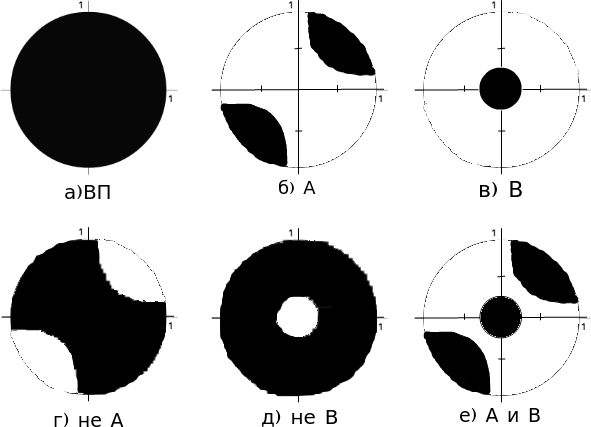
\includegraphics[width=.7\textwidth]{./pictures/2_18.png}
  \caption{Вероятностное пространство и события из задачи 2.18}
  \label{fig:218}
\end{figure}

\begin{enumerate}[label=\alph*)]
\item $ A =
\{ (x, y), x^2 + y^2 \leq 1, xy \leq \frac{ 1 }{ 8 } \} $ (\ref{fig:218}, г));

\item $ B =
\{ (x, y), x^2 + y^2 \leq \frac{ 1 }{ 4 } \} $ (\ref{fig:218}, в));

\item событие $ \overline{ A } $ означает, что событие А не произошло,то есть произведение координат точки превышает 1/8 (\ref{fig:218}, б)):
$$ \overline{ A } =
\{ (x, y), xy > 1/8, x^2 + y^2 \leq 1 \}.$$

Событие $ \overline{ B } $ означает, что точка не оказалась внутри круга радиуса 1/4 (\ref{fig:218}, д)):
$$ \overline{ B } =
\{ (x, y), 1 \geq x^2 + y^2 > \frac{ 1 }{ 4 } \}.$$

Событие $ A \cap B $ означает, что произошло и событие A, и событие B.
Отсюда имеем, что произведение координат точки не должно превышать 1/8, а сумма квадратов координат должна быть не больше 1/4 (\ref{fig:218}, е)), т.е.
$$ A \cap B =
\{ (x, y), x^2 + y^2 \leq \frac{ 1 }{ 4 }, xy \leq \frac{ 1 }{ 8 } \}.$$
\end{enumerate}

\addcontentsline{toc}{chapter}{Занятие 3. Классическое определение вероятности}
\chapter*{Занятие 3. Классическое определение вероятности}

\addcontentsline{toc}{section}{Контрольные вопросы и задания}
\section*{Контрольные вопросы и задания}

\subsubsection*{Приведите определение вероятностного эксперимента, вероятностного пространства, случайного события.}

Вероятностным экспериментом называется явление, исход которого для нас не определён, и который можно повторить любое число раз независимым образом.

Вероятностное пространство --- совокупность всех исходов вероятностного эксперимента, $\Omega$.

Случайное событие --- подмножество всех исходов вероятностного эксперимента.

\subsubsection*{Как вычислить вероятность события в случае, когда вероятностное пространство состоит из конечного количества равновероятных элементарных событий?}

В этом случае вероятность любого события A вычисляется по формуле
$$ P(A) =
\frac{ |A| }{ |\Omega| },$$
называемой классическим определением вероятности.

\subsubsection*{Запишите формулу включений и исключений.}

Если
$ B_1, B_2,  \dotsc , B_m $ --- некоторые события, то имеет место равенство
$ P\{ \bigcup \limits_{i=1}^m B_i \} =
\sum \limits_{i=1}^m P \{ B_i \} -
\sum \limits_{ 1 \leq i_1 < i_2 \leq m } \{ B_{ i_1 } \cap B_{ i_2 } \} + \dotsc + \\
+ (-1)^{k-1} \sum \limits_{ 1 \leq i_1 < i_2 < \dotsc < i_k \leq m } P \{ B_{ i_1 } \cap B_{ i_2 } \cap \dotsc \cap B_{ i_k } \} + \dotsc + \\
+ (-1)^{m-1} P \{ B_1 \cap B_2 \cap \dotsc \cap B_m \}.$

\addcontentsline{toc}{section}{Аудиторные задачи}
\section*{Аудиторные задачи}

\subsubsection*{3.3}

\textit{Задание.} Пусть A и B такие события, что
$$P \left( A \cap B \right) = \frac{1}{4},
P \left( \overline{A} \right) = \frac{1}{3},
P \left( B \right) = \frac{1}{2}. $$
Вычислите $P \left( A \cup B \right)$.

\textit{Решение.} Вычислим вероятность события A:
$$P \left( A \right) =
1 - P \left( \overline{A} \right) =
1 - \frac{1}{3} =
\frac{2}{3}.$$

Так как события независимы, то вероятность пересечения событий равна произведению пересечений, т.е
$P \left( A \cap B \right) = P \left( A \right) P \left( B \right) $.

Вычислим вероятность объединения:
$$P \left( A \cup B \right) =
P \left( A \right) + P \left( B \right) - P \left( A \cap B \right) =
\frac{2}{3} + \frac{1}{2} - \frac{1}{4} =
\frac{8+6-3}{12} =
\frac{11}{12}.$$

\subsubsection*{3.4}

\textit{Задание.} Было подброшено три монеты.
Найдите вероятности событий:
\begin{enumerate}[label=\alph*)]
\item A = {хотя бы одна из монет выпала гербом};
\item B = {выпало ровно два герба};
\item C = {выпало не меньше двух гербов}.
\end{enumerate}

\textit{Решение.} На первой монете может появиться или герб, или цифра.
Аналогичные два элементарных исхода возможны при подбрасывании остальных монет.
Таким образом, общее число возможных элементарных исходов испытания равно $2 \cdot 2 \cdot 2 = 8$.
Эти исходы равновероятны.

\begin{enumerate}[label=\alph*)]
\item Рассмотрим событие $ \overline{A} = $ \{все монеты выпали решкой\} = \{ЦЦЦ\}.
Мощность этого события равна $\left| \overline{A} \right| = 1$.
Таким образом, вероятность события $ \overline{A} $ будет
$$P \left( A \right) =
\frac{ \left| \overline{A} \right| }{ \left| \Omega \right| } =
\frac{1}{8}.$$
Тогда вероятность необходимого события
$$P \left( A \right) =
1 - P \left( \overline{A} \right) =
1 - \frac{1}{8} =
\frac{7}{8};$$
\item благоприятствующим интересующему нас событию (выпало ровно два герба) являются следующие исходы: ГГЦ, ГЦГ, ЦГГ.

Искомая вероятность равна
$$P \left( B \right) =
\frac{3}{8};$$

\item опишем событие С = \{выпало не меньше двух гербов\} = $B \cup $ \{ГГГ\}.

Искомая вероятность равна
$$P \left( C \right) =
\frac{4}{8} =
\frac{1}{2}.$$
\end{enumerate}

\subsubsection*{3.5}

\textit{Задание.} Подброшено 12 игральных кубиков.
Найдите вероятность того, что каждое из очков $1, 2, \dotsc, 6$ выпало дважды.

\textit{Решение.}
На выпавшей грани <<первого>> игрального кубика может появиться одно очко, два очка, $ \dotsc $, шесть очков.
Аналогичные шесть элементарных исходов возможны при бросании остальных кубиков.
Таким образом, общее число возможных элементарных исходов испытания равно $6 \cdot 6 \cdot \dotsc \cdot 6 = 6^{12}$.
Эти исходы в силу симметрии кубиков равновероятны.

Благоприятствующим интересующему нас событию
(каждое из очков выпадет дважды)
является $C_{12}^2 \cdot C_{10}^2 \cdot C_8^2 \cdot C_6^2 \cdot C_4^2 \cdot C_2^2$ исходов.

Искомая вероятность равна отношению числа исходов, благоприятствующих событию,
к числу всех возможных элементарных исходов:
$$P =
\frac{C_{12}^2 \cdot C_{10}^2 \cdot C_8^2 \cdot C_6^2 \cdot C_4^2 \cdot C_2^2}{6^{12}}.$$

\subsubsection*{3.6}

\textit{Задание.}
Игральный кубик изготовлено так,
что вероятность выпадения каждой грани пропорциональна количеству очков, изображённой на этой грани.
Вычислите вероятность того, что при подбрасывании такого игрального кубика выпадет чётное количество очков.

\textit{Решение.} Вероятность выпадения единицы пропорциональна единице, т.е. равна n, где n --- любое натуральное число.
Вероятность выпадения двойки равна $2 n$, тройки --- $3 n$, четвёрки --- $4 n$, пятёрки --- $5 n$ и шестёрки --- $6 n$.
Вероятность выпадения хоть какого-то числа равна единице, т.е. сумма вероятностей выпадения всех граней равна единице: $n + 2 n + 3 n + 4 n + 5 n + \\ + 6 n = 21 n = 1$.
Отсюда
$$n =
\frac{1}{21}.$$

Интересующие нас события: выпадет 2 очка, 4 очка или 6 очков.
2 очка может выпасть с вероятностью
$$ P \left( 2 \right) =
2 \cdot \frac{1}{21} =
\frac{2}{21}.$$
4 очка может выпасть с вероятностью
$$ P \left( 4 \right) =
4 \cdot \frac{1}{21} =
\frac{4}{21}.$$
6 очков может выпасть с вероятностью
$$ P \left( 6 \right) =
6 \cdot \frac{1}{21} =
\frac{6}{21}.$$

Вероятность выпадения чётного числа равна сумме вероятностей их выпадения:
$$P \left( 2, 4, 6 \right) =
\frac{2}{21} + \frac{4}{21} + \frac{6}{21} =
\frac{12}{21}.$$

\subsubsection*{3.7}

\textit{Задание.} Найдите вероятность того, что наугад выбранное число из множества $\{ 1, 2, \dotsc, 100!\}$ делится:
\begin{enumerate}[label=\alph*)]
\item на 2;
\item на 2 и на 3;
\item хотя бы на одно из чисел 2, 3, или 5.
\end{enumerate}

\textit{Решение.} Всего чисел $100!$.
\begin{enumerate}[label=\alph*)]
\item На 2 делится каждое второе число, т.е. количество чисел, которые делятся на 2, равно
$$\frac{100!}{2}.$$
Вероятность выбора чётного числа равна
$$P =
\frac{ \frac{100!}{2} }{100!} =
\frac{1}{2};$$

\item на 2 и на 3 делится каждое шестое число, т.е. их всего
$$ \frac{100!}{6}.$$
Тогда вероятность выбора числа, которое делится и на 2, и на 3, равна
$$P =
\frac{ \frac{100!}{6} }{100!} =
\frac{1}{6};$$

\item на 2 делится каждое второе число, на 3 --- каждое третье, на 5 --- каждое пятое.
Используем формулу включений-исключений:
$$P =
\frac{1}{2} + \frac{1}{3} + \frac{1}{5} - \frac{1}{6} - \frac{1}{10} - \frac{1}{15} + \frac{1}{30} =
\frac{15+10+6-5-3-2+1}{30} =
\frac{22}{30} =
\frac{11}{15}.$$
\end{enumerate}

\subsubsection*{3.8}

\textit{Задание.} В лифт девятиэтажного дома зашло пятеро человек.
Известно, что каждый из них с одинаковой вероятностью может выйти на любом этаже, начиная со второго.
Найдите вероятность того, что:
\begin{enumerate}[label=\alph*)]
\item все пятеро выйдут на 5-м этаже;
\item все пятеро выйдут на одном и том же этаже;
\item все пятеро выйдут на разных этажах;
\item двое людей выйдут на 4-м этаже, двое --- на 7-м и один человек выйдет на 9-м этаже.
\end{enumerate}

\textit{Решение.} Каждый из пяти человек может выйти на любом из восьми этажей.
Тогда всего есть $8 \cdot 8 \cdot 8 \cdot 8 \cdot 8 = 8^5$ вариантов.

\begin{enumerate}[label=\alph*)]
\item Все пять человек могут выйти на пятом этаже одним способов.
Тогда вероятность этого события равна
$$P =
\frac{1}{8^5};$$

\item все пять человек могут выйти на одном и том же этаже восемью способами.
Тогда вероятность этого события равна
$$P =
\frac{8}{8^5} =
\frac{1}{8^4};$$

\item первый человек может выйти на любом из восьми этажей, второй --- на любом из оставшихся семи,
третий --- на любом из оставшихся шести, четвёртый --- пяти, и наконец пятый --- на оставшихся четырёх этажах.
Тогда вероятность равна
$$P =
\frac{8 \cdot 7 \cdot 6 \cdot 5 \cdot 4}{8^5} =
\frac{7 \cdot 6 \cdot 5 \cdot 4}{8^4};$$

\item на четвёртом этаже могут выйти 2 человека из пяти $ \left( C_5^2 \right) $.
На седьмом этаже --- двое из оставшихся трёх человек.
Это $C_3^2$.
На девятом --- один человек из одного.
Это один способ.
Тогда вероятность равна
$$P =
\frac{C_5^2 \cdot C_3^2}{8^5}.$$
\end{enumerate}

\subsubsection*{3.9}

\textit{Задание.} Из колоды карт наугад выбирают 3 карты (без возвращения).
Найдите вероятность того, что среди этих карт:
\begin{enumerate}[label=\alph*)]
\item окажется ровно одни туз;
\item окажется хотя бы один туз;
\item окажется тройка, семёрка, туз.
\end{enumerate}

\textit{Решение.} Всего в колоде 52 карты.
Тогда есть 4 масти по 13 карт в каждой.
3 карты из 36 можно выбрать $C_{52}^3$ способами.

\begin{enumerate}[label=\alph*)]
\item В колоде есть 4 туза.
Один из них можно выбрать $C_4^1$ способами.
Остаётся выбрать две карты из $52-4=48$.
Это можно сделать $C_{48}^2$ способами.
Тогда вероятность выбрать 3 карты так, что среди них окажется ровно 1 туз, равна
$$P =
\frac{C_4^1 \cdot C_{48}^2}{C_{52}^3};$$

\item $B =$ \{среди этих карт окажется хотя бы 1 туз\}.
Рассмотрим противоположное событие: $ \overline{B} =$ \{среди трёх карт нет тузов\}.
Вероятность этого события равна
$$P \left( \overline{B} \right) =
\frac{C_{48}^3}{C_{52}^3}.$$
Тогда вероятнотсь интересующего нас события равна
$$P \left( B \right) =
1 - P \left( \overline{B} \right) =
1 - \frac{C_{48}^3}{C_{52}^3};$$

\item есть 4 варианта выбрать тройку, 4 выбрать семёрку и 4 --- туз.
Первой картой может быть тройка, семёрка или туз ($4 \cdot 3 = 12$ карт из 52).
Далее должна быть одна из восьми карт (т.е. 8 вариантов из оставшихся 51 карты).
Последней картой может быть любая из четырёх (из 50 карт).
По правилу произведения имеем
$$P =
\frac{12}{52} \cdot \frac{8}{51} \cdot \frac{4}{50}.$$
\end{enumerate}

\subsubsection*{3.10}

\textit{Задание.} В партии, что состоит из $N$ деталей, есть $M$ бракованных.
Найдите вероятность того, что среди $n \, \left( n < N \right)$ наугад выбранных деталей окажется:
\begin{enumerate}[label=\alph*)]
\item $m \, \left( m < M \right) $ бракованных;
\item не больше $m$ бракованных.
\end{enumerate}

\textit{Решение.} Пространство элементарных событий $ \Omega $ является множеством n-элементных подмножеств множества из $N$ элементов.
Значит, $| \Omega | = C_N^n$.

\begin{enumerate}[label=\alph*)]
\item Посчитаем число исходов,
благоприятствующих интересующему нас событию
(среди $n$ деталей ровно $m$ бракованных):
$m$ бракованных деталей можно взять из $M$ бракованных деталей $C_M^m$ способами;
при этом остальные $n - m$ деталей не должны быть бракованными;
взять же $n - m$ не бракованных деталей из $N - M$ не бракованных деталей можно $C_{N-M}^{n-m}$ способами.
Следовательно, число благоприятствующих исходов равно $C_M^m C_{N-M}^{n-m}$.

Искомая вероятность равна отношению числа исходов, благоприятствующих событию, к числу всех элементарных исходов:
$$P =
\frac{C_M^m C_{N-M}^{n-m}}{C_N^n};$$

\item посчитаем число исходов,
благоприятствующих интересующему нас событию
(среди $n$ деталей от нуля до $m$ бракованных):
от нуля до $m$ бракованных деталей можно взять из $M$ бракованных деталей $ \sum \limits_{i=0}^m C_M^i$ способами;
при этом остальные от $n - m$ до $n$ деталей не должны быть бракованными;
взять же от $n - m$ до $n$ не бракованных деталей из $N - M$ не бракованных деталей можно $ \sum \limits_{i=0}^m C_{N-M}^{n-i}$ способами.
Следовательно, число благоприятствующих исходов равно $ \sum \limits_{i=0}^m C_M^i C_{N-M}^{n-i}$.

Искомая вероятность равна отношению числа исходов, благоприятствующих событию, к числу всех элементарных исходов:
$$P =
\frac{ \sum \limits_{i=0}^m C_M^i C_{N-M}^{n-i}}{C_N^n}.$$
\end{enumerate}

\subsubsection*{3.11}

\textit{Задание.} В купейный вагон (9 купе по 4 места в каждом) семи пассажирам продано семь билетов.
Найдите вероятность того, что занятыми окажутся:
\begin{enumerate}[label=\alph*)]
\item ровно два купе;
\item ровно три купе.
\end{enumerate}

\textit{Решение.}
Любой из семи пассажиров может занять любое из четырёх мест в любом из девяти купе (всего мест $4 \cdot 9 = 36$).
Тогда общее число элементарных исходов --- $C_{36}^7$.

\begin{enumerate}[label=\alph*)]
\item Для начала необходимо выбрать 2 вагона из девяти.
Это $C_9^2$ способа.
Далее нужно разместить 7 пассажиров среди восьми мест в этих двух вагонах ($C_{8}^7$ способов).
Тогда число благоприятствующих исходов равно $С_9^2 C_8^7$.

Вероятность указанного события равна
$$P =
\frac{С_9^2 C_8^7}{C_{36}^7};$$

\item для начала нужно выбрать 3 вагона из девяти.
Это $C_9^3$ способа.
Далее нужно разместить 7 пассажиров среди двенадцати мест в этих трёх вагонах ($C_{12}^7$ способов).
Тогда число благоприятствующих исходов равно $C_9^3 C_{12}^7$.

Вероятность указанного события равна
$$P =
\frac{C_9^3 C_{12}^7}{C_{36}^7}.$$
\end{enumerate}

\subsubsection*{3.12}

\textit{Задание.} Шутник Петя написал письма $n$ адресатам, в каждый конверт вложил по одному письму, а потом наугад написал на каждом из конвертов один из $n$ адресов.
Найдите вероятность того, что:
\begin{enumerate}[label=\alph*)]
\item хотя бы одно письмо придёт по назначению;
\item ровно $m$ писем придут по назначению.
\end{enumerate}

\textit{Решение.} Разложить $n$ писем в $n$ конвертов можно $n!$ способами.

\begin{enumerate}[label=\alph*)]
\item Найдём вероятность того, что ни одно письмо не попадёт в конверт с правильным адресом, а затем вычтем её из $1$.

Из общего числа способов необходимо вычесть число тех вариантов, при которых первое письмо попадает в 1-й конверт,
все способы, при которых второе письмо попадает во 2-й конверт и т.д.

Письмо, которое будет вложено в конверт с правильным адресом, можно выбрать $n$ способами;
остальные $n - 1$ письмо можно вложить в $n - 1$ конверт $ \left( n - 1 \right)!$ способами,
поэтому общее число вариантов размещения писем по конвертам равно $n \cdot \left( n - 1 \right)! = n!$.
Вычитая это число из общего числа возможных вариантов размещения писем по конвертам, равного $n!$,
мы не оставляем ни одного варианта.
Вариант, в котором, например, первое письмо попадает в 1-й конверт, а второе письмо --- во 2-й, мы вычитаем дважды.

Чтобы найти, сколько вариантов мы вычли слишком большое число раз, заметим, что существует 
$$C_n^2 =
\frac{n!}{2! \left( n-2 \right)!} =
\frac{n \left( n-1 \right) }{2!}$$
пар писем, и если письма, образующие пару, вложены в конверты с правильными адресами, то остальные $n - 2$ письма можно распределить по конвертам
$$\frac{n \left( n-1 \right)}{2!} \cdot \left( n-2 \right)! =
\frac{n!}{2!}$$
способами.

Прибавив число способов распределения писем в конверты, при которых два письма вложены в свои конверты, мы получим всего
$$n! - n! + \frac{n!}{2!}$$
вариантов размещения писем по конвертам.

Но теперь это слишком много,
так как все варианты, при которых в свои конверты вложены три письма, не были учтены
(мы вычли число таких вариантов трижды, а затем прибавили его столько раз,
сколько пар писем можно образовать из трёх писем, т.е. три раза).
Следовательно, мы должны вычесть число способов, которыми можно вложить в конверты с правильными адресами три письма, т.е.
$$C_n^3 \cdot \left( n-3 \right)! =
\frac{n!}{\left( n-3 \right)! 3!}\cdot \left( n-3 \right)! =
\frac{n!}{3!}$$
способов.

Теперь мы вычли слишком много раз число способов,
которыми можно вложить в конверты с правильными адресами четыре письма и т.д.
Таким образом, число способов, которыми письма можно разложить по конвертам так, что ни одно письмо не окажется в конверте с правильным адресом, равно
$$n! - n! + \frac{n!}{2!} - \frac{n!}{3!} + \dotsc + \left( -1 \right)^{n+1} \left( \frac{1}{n!} \right),$$
а вероятность этого события равна этому числу, делённому на $n!$, т.е. равна числу
$$1 - 1 + \frac{1}{2!} + \dotsc + \left( -1 \right)^{n+1} \frac{1}{n!}.$$
Следовательно, вероятность того, что по крайней мере одно письмо окажется в конверте с правильным адресом, равна
$$P =
1 - \frac{1}{2!} + \frac{1}{3!} - \dotsc + \left( -1 \right)^{n+1} \frac{1}{n!};$$

\item найдём вероятность того, что $n - m$ писем не попадут в конверты с правильными адресами, а затем вычтем её из 1.

Письма, которые будут вложены в конверты с правильными адресами,
можно выбрать $C_n^m$ способами;
остальные $n - m$ писем можно вложить в $n - m$ конвертов $ \left( n-m \right)!$ способами,
поэтому общее число вариантов размещения писем по конвертам равно $$C_n^m \cdot \left( n-m \right)!.$$

Аналогично пункту а) получаем, что число способов, которыми письма можно разложить по конвертам так, что ровно $m$ писем окажется в конверте с правильным адресом, равно
$$C_n^m
\left( \left( n-m \right)! - \left( n-m \right)! + \frac{ \left(n-m \right)!}{2!} - \frac{ \left( n-m\right)!}{3!} + \dotsc \right),$$
а вероятность этого события равна этому числу, делённому на $n!$, т.е. равна числу
\begin{equation*}
\begin{split}
C_n^m \cdot \frac{1}{n!}
\left( \left( n-m \right)! - \left( n-m \right)! + \frac{ \left(n-m \right)!}{2!} - \frac{ \left( n-m\right)!}{3!} + \dotsc \right) = \\
= \frac{1}{m! \left( n-m \right)!}
\left( \left( n-m \right)! - \left( n-m \right)! + \frac{ \left(n-m \right)!}{2!} - \frac{ \left( n-m\right)!}{3!} + \dotsc \right) = \\
= \frac{1}{m!} \left( \frac{1}{2!} - \frac{1}{3!} + \dotsc \right).
\end{split}
\end{equation*}

Следовательно, вероятность того, что ровно $m$ писем окажется в конвертах с правильными адресами, равна
$$P =
1 - \frac{1}{m!} \left( \frac{1}{2!} - \frac{1}{3!} + \dotsc \right).$$

\paragraph*{Число встреч}

В задаче используется понятие <<число встреч>>.
Под ним понимается число перестановок множества $\{ 1, \dotsc, n \}$ с заданным числом неподвижных элементов.
Для $n \geq 0$ и $0 \leq k \leq n$ число встреч $D_{n, k}$ --- это число перестановок $\{ 1, \dotsc, n \}$,
содержащих ровно $k$ элементов, не изменивших положение в перестановке.

\begin{figure}[h!]
  \centering
  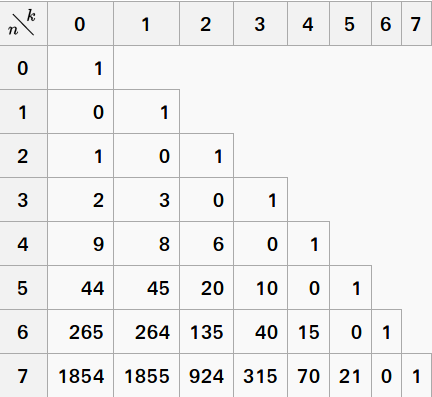
\includegraphics[width=.7\textwidth]{./pictures/3_12.png}
  \caption{Фрагмент таблицы числа встреч}
  \label{fig:312}
\end{figure}

Числа в первом столбце $ \left( k=0 \right) $ показывают число беспорядков (рис. \ref{fig:312}).
Так,
$D_{0, 0} = 1, D_{1, 0} = 0, D_{n+2, 0} = \left( n+1 \right) \left( D_{n+1, 0} + D_{n, 0} \right)$ для неотрицательного $n$.

Выберем $m$ фиксированных элементов из $n$, затем посчитаем число беспорядков оставшихся $n - m$ элементов.
Это будет
$$ \left( n-m \right)! \sum \limits_{k=0}^{n-m} \frac{ \left( -1 \right)^k}{k!}.$$

$$D_{n ,m} =
C_n^m D_{n-m, 0} =
\frac{n!}{m!} \sum \limits_{k=0}^{n-m} \frac{ \left( -1 \right)^k}{k!}.$$
\end{enumerate}

\subsubsection*{3.13}

\textit{Задание.} (Статистика Максвелла-Больцмана). Каждая из $n$ разных частиц наугад попадает в одну из $N$ ячеек.
\begin{enumerate}[label=\alph*)]
\item Найдите вероятность того, что в первой, второй и т.д., N-ой ячейке будет соответственно $n_1, n_2, \dotsc, n_N$ частиц;
\item найдите вероятность $p_k$ того, что данная ячейка содержит $k$ частиц;
\item *докажите, что если $n$ и $N$ стремятся к бесконечности так, что
$$ \frac{n}{N} \rightarrow \lambda,$$
то
$$p_k \rightarrow \frac{ \lambda^k}{k!}e^{- \lambda};$$
\item найдите вероятность того, что в каждой ячейке есть хотя бы одна частица;
\item найдите вероятность того, что занято ровно $r$ ячеек.
\end{enumerate}

\textit{Решение.} В случаях а), б) и д) вероятность желаемого события оценивается по формуле
$$p =
\frac{r}{m}.$$
Для каждой из $n$ разных частиц есть $N$ вариантов попасть в одну из ячеек.
Поэтому по правилу умножения имеем общее количество вариантов $m = N^n$.
Вычислим количество $r$ вариантов, что отвечают каждому из событий, указанных в условии задачи.

\begin{enumerate}[label=\alph*)]
\item Существует $C_n^{n_1}$ способов, которыми можно отобрать $n_1$ частицу в первую ячейку.
Аналогично, количество способов отобрать $n_2$ частицы во вторую ячейку среди $n - n_1$ частицы, которые остались, равно $C_{n-n_1}^{n_2}$.
Подобным же образом отбираются частицы и для других ячеек.
Поэтому событию способствуют
\begin{equation*}
\begin{split}
r =
C_n^{n_1} \cdot C_{n-n_1}^{n_2} \cdot C_{n - n_1 - n_2}^{n_3} \cdot \dotsc = \\
= \frac{n!}{n_1! \left( n-n_1 \right)!}
\cdot \frac{ \left( n-n_1 \right)!}{n_2! \left( n - n_1 - n_2 \right)!}
\cdot \frac{ \left( n - n_1 - n_2 \right)!}{n_3! \left( n - n_1 - n_2 - n_3 \right)!} \cdot \dotsc = \\
= \frac{n!}{n_1! n_2! n_3! \dotsc n_N!}
\end{split}
\end{equation*}
способов.

Тогда вероятность равна
$$p =
\frac{\frac{n!}{n_1! n_2! n_3! \dotsc n_N!}}{N^n} =
\frac{n!}{N^n \cdot n_1! n_2! n_3! \dotsc n_N!};$$

\item сначала нужно отобрать $k$ частиц в фиксированную ячейку
(это можно сделать $C_n^k$ способами),
а потом $n - k$ частиц распределить среди $N - 1$ ячейки
($ \left( N - 1\right)^{n-k}$ способов).
По правилу умножения имеем $r = C_n^k \cdot \left( N-1 \right)^{n-k}$ способов.

Тогда вероятность равна
$$p_k =
\frac{C_n^k \cdot \left( N-1 \right)^{n-k}}{N^n}ж$$

\item *распишем $p_k$:
\begin{equation*}
\begin{split}
p_k =
\frac{C_n^k \left( N-1 \right)^{n-k}}{N^n} =
\frac{n! \left( N-1 \right)^{n-k}}{k! \left( n-k \right)! \cdot N^n} = \\
= \frac{n! \left( N-1 \right)^n}{k! \left( n-k \right)! \cdot N^n \left( N-1 \right)^k} =
\frac{n!}{k! \left( n-k \right)! \left( N-1 \right)^k} \cdot \left( \frac{N-1}{N} \right)^n = \\
= \frac{ \left( n-k \right)! \left( n-k+1 \right) \dotsc n}{k! \left( n-k \right)! \left( N-1 \right)^k} \cdot \left(\frac{N-1}{N} \right)^n =
\frac{ \prod \limits_{i=0}^{k-1} \left( n-i \right) }{k! \left( N-1 \right)^k} \cdot \left( \frac{N-1}{N} \right)^n = \\
= \frac{ \prod \limits_{i=0}^{k-1} \left( \frac{n-i}{N-1} \right)}{k!} \cdot \left( 1 - \frac{1}{N} \right)^n.
\end{split}
\end{equation*}

Умножим и поделим последнюю скобку на $n$.
Получим:
\begin{equation*}
\begin{split}
p_k =
\frac{ \prod \limits_{i=0}^{k-1} \left( \frac{n-i}{N-1} \right)}{k!} \cdot \left( 1 - \frac{ \frac{n}{N} }{n} \right)^n.
\end{split}
\end{equation*}

Возьмём предел полученного выражения при 
$$ \frac{n}{N} \rightarrow \lambda.$$
Получим:
$$ \lim \limits_{ \frac{n}{N} \rightarrow \lambda } p_k =
\lim \limits_{ \frac{n}{N} \rightarrow \lambda }
\left( \frac{ \prod \limits_{i=0}^{k-1} \left( \frac{n-i}{N-1} \right)}{k!} \cdot \left( 1 - \frac{ \frac{n}{N} }{n} \right)^n \right) =
\frac{ \lambda^k}{k!} \exp \left( - \lambda \right);$$

\item вероятность соответственного события вычисляется с помощью формулы включений и исключений:
$P \left\{ \bigcup \limits_{i=1}^m B_i \right\} =
\sum \limits_{i=1}^m P \left\{ B_i \right\} - \\
- \sum \limits_{1 \leq i_1 < i_2 \leq m} P \left\{ B_{i_1} \cap B_{i_2} \right\} + \dotsc + \\
+ \left( -1 \right)^{k-1} \sum \limits_{1 \leq i_1 < i_2 < \dotsc < i_k \leq m} P \left\{ B_{i_1} \cap B_{i_2} \cap \dotsc \cap B_{i_k} \right\} + \dotsc + \\
+ \left( -1 \right)^{m-1} P \left\{ B_1 \cap B_2 \cap \dotsc \cap B_m \right\}$.
Обозначим через $B_i$ событие <<ячейка $i$ не содержит частиц>>.
Тогда $p = 1 - P \left\{ \bigcup \limits_{i=1}^N B_i \right\}$.
Для любых $i = 1, \dotsc, N, \, 1 \leq \\
\leq i_1 < i_2 < \dotsc i_j \leq N$
$$P \left\{ B_i \right\} =
\frac{ \left( N-1 \right)^m}{N^m}, \,
P \left\{ B_{i_1} \cap B_{i_2} \cap \dotsc \cap B_{i_j} \right\} =
\frac{ \left( N-j \right)^m}{N^m}, \,
j = 2, 3, \dotsc, N-1$$
($j$ ячеек являются пустыми; $m$ разных частиц можно разместить в $N - j$ ячейках $ \left( N-j \right)^m$ способами).
Количество слагаемых в соответствующей сумме равно $C_n^j$.
Согласно с формулой включений и исключений имеем окончательный ответ
$$p =
1 - \frac{1}{N^m} \cdot \left[ C_N^1 \cdot \left( N-1 \right)^m - C_N^2 \cdot \left( N-2 \right)^m + \dotsc + \left( -1 \right)^N \cdot C_N^{N-1} \cdot 1^m \right];$$

\item решение задачи разбиваем на два шага: сначала выбираем $r$ ячеек из $N$, которые будут занятыми (это можно сделать $C_N^r$ способами),
а потом размещаем $n$ разных частиц в $r$ ячеек таким образом, чтобы ни одна из них не была пустой ( подобная задача решена в пункте г) по формуле включений и исключений).
Поэтому окончательно имеем
$r =
C_N^r \times \\
\times \left[ r^n - C_r^1 \cdot \left( r-1 \right)^n + C_r^2 \cdot \left( r-2 \right)^n - \dotsc + \left( -1 \right)^{r-1} \cdot C_r^{r-1} \cdot 1^n \right]$.
\end{enumerate}

\addcontentsline{toc}{section}{Дополнительные задачи}
\section*{Дополнительные задачи}

\subsubsection*{3.14}

\textit{Задание.} Каждое из двух чисел $a, b$ наугад выбирают из множества $ \left\{ 1, 2, \dotsc, n \right\}$.
Вычислите вероятность того, что одно из них делится на другое.
Найдите предел этой вероятности при $n \rightarrow \infty$.

\textit{Решение.} Вероятность будет равна
$$P =
\frac{k}{m},$$
где $k$ --- сумма количества делителей каждого числа из множества  $ \left\{ 1, 2, \dotsc, n \right\}$, $m$ --- количество разных пар чисел.

Найдём $m$.
Это будет число комбинаций из $n$ по $2$: $C_n^2$.

Найдём количество множителей натурального числа.
Пусть
$n =
p_1^{ \alpha_1} \cdot p_2^{ \alpha_2} \cdot \\
\cdot \dotsc \cdot p_s^{ \alpha_s}$
--- каноническое разложение на простые множители натурального числа $n$.
Тогда число $ \tau \left( n \right) $ натуральных делителей числа $n$ выражается формулой
$ \tau \left( n \right) =
\left( \alpha_1 + 1 \right) \dotsc \left( \alpha_s + 1 \right)$.

Каждый натуральный делитель $d$ числа $n$
может быть записан в виде
$d = p_1^{ \delta_1} p_2^{ \delta_2} \dotsc p_s^{ \delta_s}$, где $ \delta_i$ ---
целые числа, удовлетворяющие условиям
$ \delta_i \in  \\
\in \left\{ 0, 1, \dotsc, \alpha_i \right\}$
для $i = 1, 2, \dotsc, s$.

Докажем это утверждение.
Пусть $d$ есть какой-либо натуральный делитель $n$.
Так как каждый простой делитель числа $d$
является делителем числа $n$, то ввиду
$n =
p_1^{ \alpha_1} \cdot p_2^{ \alpha_2} \cdot \dotsc \cdot p_s^{ \alpha_s}$
в разложении $d$ на простые множители могут встречаться только числа множества $ \left\{ p_1, \dotsc, p_s \right\}$.
Поэтому число $d$ представимо в виде $d = p_1^{ \delta_1} p_2^{ \delta_2} \dotsc p_s^{ \delta_s}$, где $ \delta_i$,
причём показатели $ \delta_i$ должны удовлетворять условиям
$ \delta_i \in \left\{ 0, 1, \dotsc, \alpha_i \right\}$ для $i = 1, 2, \dotsc, s$.

С другой стороны, если $d$ представимо в виде
$d =
p_1^{ \delta_1} p_2^{ \delta_2} \dotsc p_s^{ \delta_s}$
и показатели удовлетворяют условиям
$ \delta_i \in \left\{ 0, 1, \dotsc, \alpha_i \right\}$
для $i = 1, 2, \dotsc, s$, то
$n =
d \left( p_1^{ \alpha_1 - \delta_1} \dotsc p_s^{ \alpha_s - \delta_s} \right) \left( \alpha_i - \delta_i \geq 0 \right)$,
т.е. $d$ является натуральным делителем числа $n$.

Чтобы найти число всех натуральных делителей числа $n$,
достаточно посчитать число всевозможных упорядоченных наборов
$ \delta_1, \dotsc, \delta_s$, удовлетворяющих условиям
$ \delta_i \in \left\{ 0, 1, \dotsc, \alpha_i \right\}$ для $i = 1, 2, \dotsc, s$.
Ввиду условий $ \delta_i$ может принимать $ \alpha_i + 1$ значение,
выборы различных значений $ \delta_1, \dotsc, \delta_s$
не зависят один от другого
и в силу единственности разложения на простые множители разным наборам соответствуют различные делители $n$.
Следовательно, число всех натуральных делителей числа $n$ равно
$ \left( \alpha_1 + 1 \right) \dotsc \left( \alpha_s + 1 \right)$.

Можно оценить количество делителей числа.
В терминах о-малое,
функция делителей удовлетворяет неравенству для всех $ \epsilon > 0, \, d \left( n \right) = o \left( n^{\epsilon} \right)$.

Тогда имеем вероятность
$$P =
\frac{ \sum \limits_{i=1}^n i^{\epsilon}}{C_n^2} \, \forall \epsilon > 0.$$

\addcontentsline{toc}{section}{Домашнее задание}
\section*{Домашнее задание}

\subsubsection*{3.15}

\textit{Задание.} Докажите, что для произвольных событий A и B
$ P( AB ) = \\
= 1 - P\left( \overline{ A } \right) - P \left( \overline{ B } \right) + P \left( \overline{ A } \, \overline{ B } \right) $.

\textit{Решение.}
$ P( AB ) =
P(A) + P(B) - P \left( A \cup B \right) = \\
= 1 - P \left( \overline{ A }\right) + 1 - P \left( \overline{ B } \right) - \left( 1 - P \left( \overline{ A \cup B } \right) \right) =
1 - P \left( \overline{ A } \right) + 1 - P \left( \overline{ B } \right) - 1 + P \left( \overline{ A } \, \overline{ B } \right) = \\
= 1 - P \left( \overline{ A } \right) - P \left( \overline{ B } \right) + P \left( \overline{ A } \, \overline{ B } \right) $.

\subsubsection*{3.16}

\textit{Задание.} Подбрасывают 4 игральных кубика.
Найдите вероятность того, что на них выпадет одинаковое количество очков.

\textit{Решение.} На выпавшей грани <<первого>> игрального кубика может появиться одно очко, два очка,  $ \dotsc $ , шесть очков.
Аналогичные шесть элементарных исходов возможны при бросании остальных кубиков.
Таким образом, общее число возможных элементарных исходов испытания равно $ 6 \cdot 6 \cdot 6 \cdot 6 = 1296 $.
Эти исходы в силу симметрии кубиков равновероятны.

Благоприятствующие интересующему нас событию
(на всех гранях появится одинаковое количество очков)
являются следующие шесть исходов
(первым записано число очков,
выпавших на <<первом>> кубике,
вторым --- число очков, выпавших на <<втором>> кубике, и т.д.): 1) 1, 1, 1, 1, 2) 2, 2, 2, 2, 3) 3, 3, 3, 3, 4) 4, 4, 4, 4, 5) 5, 5, 5, 5, 6) 6, 6, 6, 6.

Искомая вероятность равна отношению числа исходов, благоприятствующих событию, к числу всех возможных элементарных исходов:
$$ P =
\frac{6}{6^4} = \frac{1}{6^3}.$$

\subsubsection*{3.17}

\textit{Задание.} Группа состоит из r студентов.
Найдите вероятность того, что по крайней мере 2 студента родились в одном и том же месяце (считайте, что все месяцы года являются равновероятными для рождения).

\textit{Решение.} Год имеет 12 месяцев.
День рождения каждого из студентов может приходиться на любой месяц года (12 вариантов).

Если студентов больше чем месяцев ($ r > 12 $), то не существует исходов, при которых в один месяц попадает один человек.
$ P = 0 $.

Рассмотрим случай, когда студентов в группе не больше чем месяцев в году ($ r \leq 12 $).
По правилу умножения существует всего $ n = 12^r $ вариантов размещения дней рождения студентов.
Найдём количество вариантов, когда никакие два студента не имеют день рождения в тот же месяц.
Для этого нужно вычислить количество способов, которыми из 12 месяцев можно выбрать упорядоченное множество из r месяцев.
Используя формулу для размещения из 12 элементов по r, имеем $ A_{12}^r $.
Поэтому
$$ P =
1 - \frac{ A_{ 12 }^r }{ 12^r }.$$

\subsubsection*{3.18}

\textit{Задание.} Сколько людей должно быть в комнате, чтобы вероятность того, что хотя бы двое из присутствовавших родились в один и тот же день года, была большей чем 1/2?

\textit{Решение.} Пусть r --- число людей, и будем считать, что все дни рождения равновероятны.
Вычислим вероятность противоположного события A = {все люди родились в разные дни}.
Число способов, благоприятствующих этому событию --- это число размещений из 365 по r.
Всего же имеется $ n = 365^r $ возможностей распределения дней рождения.
То есть
$$ P(A) =
\frac{A_{365}^r}{365^r}.$$

Вероятность интересующего нас события $ \overline{A} $ тогда равна
$$ P \left( \overline{A} \right) =
1 - P \left( A \right) =
1 - \frac{A_{365}^r}{365^r}.$$

Вычислим вероятность $ P \left( \overline{A} \right) $ для различных значений r.
\begin{equation*}
\begin{split}
r = 5 : P \left( \overline{A} \right) =
1 - \frac{A_{365}^5}{365^5} =
1 - \frac{5! \cdot C_{365}^5}{365^5} = \\
= 1 - \frac{5! \cdot \frac{365!}{5! \cdot 360!} }{365^5} =
1 - \frac{365!}{360! \cdot 365^5} =
1 - \frac{360! \cdot 361 \cdot 362 \cdot 363 \cdot 364 \cdot 365}{360! \cdot 365^5} = \\
= 1 - \frac{361 \cdot 362 \cdot 363 \cdot 364}{365^4} =
1 - \frac{1.72 \cdot 10^10}{1.77 \cdot 10^10} =
1 - 0.97 =
0.03.
\end{split}
\end{equation*}

\begin{equation*}
\begin{split}
r = 10 :
P \left( \overline{A} \right) =
1 - \frac{A_{365}^{10}}{365^{10}} =
1- \frac{10! \cdot C_{365}^{10}}{365^{10}} = \\
= 1 - \frac{10! \cdot \frac{365!}{10! \cdot 355!}}{365^{10}} =
1 - \frac{365!}{355! \cdot 365^{10}} =
0.12.
\end{split}
\end{equation*}

\begin{equation*}
\begin{split}
r = 20 :
P \left( \overline{A} \right) =
1 - \frac{A_{365}^{20}}{365^{20}} =
1 - \frac{20! \cdot C_{365}^{20}}{365^{20}} =
1 - \frac{365!}{345! \cdot 365^{20}} =
0.41.
\end{split}
\end{equation*}

\begin{equation*}
\begin{split}
r = 22 :
P \left( \overline{A} \right) =
1 - \frac{A_{365}^{22}}{365^{22}} =
1 - \frac{365!}{343! \cdot 365^{22}} =
0.48.
\end{split}
\end{equation*}

\begin{equation*}
\begin{split}
r = 23 :
P \left( \overline{A} \right) =
1 - \frac{A_{365}^{23}}{365^{23}} =
1 - \frac{365!}{342! \cdot 365^{23}} =
0.51.
\end{split}
\end{equation*}

При
$ r = 23 $
вероятность по крайней мере одного совпадения равна
$ 0.51 > \\
> 0.5 $,
то есть
$ r = 23 $ ---
наименьшее число, удовлетворяющее условиям задачи.

\subsubsection*{3.19}

\textit{Задание.} Числа $ 1, 2,  \dotsc , n $ размещены в случайном порядке.
Найдите вероятность того, что числа:
\begin{enumerate}[label=\alph*)]
\item 1 и 2;
\item 1, 2 и 3 размещены рядом в указанном порядке.
\end{enumerate}

\textit{Решение.} Пространство элементарных событий $  \Omega$ является множеством всех перестановок множества из n элементов.
Значит $ |\Omega| = n! $.

\begin{enumerate}[label=\alph*)]
\item Поскольку числа 1 и 2 стоят рядом, то их можно рассматривать как одно число (обозначим его $ n + 1 $).
Количество возможных перестановок чисел $ \{ 3, 4,  \dotsc , n + 1 \} $ равно $ \left( n - 1 \right)! $.
Тогда вероятность данного события равна:
$$ P =
\frac{ \left( n - 1 \right)! }{ n! } =
\frac{1}{n};$$

\item поскольку числа 1, 2 и 3 стоят рядом, то их можно рассматривать как одно число (обозначим его $ n + 1 $).
Количество возможных перестановок чисел $ \{ 4, 5,  \dotsc , n + 1 \} $ равно $ \left( n - 2 \right)! $.
Тогда вероятность данного события равна:
$$ P = \frac{ \left( n - 2 \right)!}{ n! } =
\frac{1}{ n (n - 1 ) }.$$
\end{enumerate}

\subsubsection*{3.20}

\textit{Задание.} Экзамен состоит из 10 вопросов, на каждый из которых нужно дать ответ <<да>> или <<нет>>.
Найдите вероятность того, что студент правильно ответил хотя бы на $ 70 \% $ вопросов, выбирая ответ наугад.
Решите задачу, если тест состоит из 30 и из 50 вопросов.

\textit{Решение.} На каждый вопрос есть возможность ответить двумя способами (<<да>> или <<нет>>).

В случае, когда экзамен состоит из десяти вопросов, пространство элементарных событий содержит $ | \Omega | = 2^{10} $ элементов.
Найдём вероятность события А = {студент правильно ответит хотя бы на 70\% вопросов из десяти}.
Ответить правильно хотя бы на 70\% вопросов означает ответить правильно хотя бы на 7 вопросов из 10, т. е. событие А допускает правильный ответ на 7, 8, 9 или 10 вопросов.
На 7 вопросов правильно можно ответить $ C_{10}^7 $ способами.
На 8 вопросов правильно можно ответить $ C_{10}^8 $ способами.
На 9 --- $ C_{10}^9 $.
Аналогично, на 10 вопросов можно дать правильный ответ $ C_{10}^{10} $ способами.
По правилу суммы имеем $ |A| = C_{10}^7 + C_{10}^8 + C_{10}^9 + C_{10}^{10} = \sum \limits_{i=7}^{10} C_{10}^i $.
Тогда вероятность события A равна
$$ P \left( A \right) =
\frac{|A|}{| \Omega |} =
\frac{ \sum \limits_{i=7}^{10} C_{10}^i}{2^{10}}.$$

Аналогично находим вероятность правильного ответа на хотя бы 70\% вопросов из тридцати и пятидесяти.

Когда всего есть 30 вопросов (событие B), то 70\% от них --- это $ 30 \cdot 0.7 = 21$ вопрос.
Тогда
$$ P \left( B \right) =
\frac{ \sum \limits_{i=21}^{30} C_{30}^i}{2^{30}}.$$

Когда всего есть 50 вопросов (событие C), то 70\% от них --- это $ 50 \cdot 0.7 = 35$ вопрос.
Тогда
$$ P \left( C \right) =
\frac{ \sum \limits_{i=35}^{50} C_{50}^i}{2^{50}}.$$

\subsubsection*{3.21}

\textit{Задание.} Список из 4N участников турнира разбито на четыре равные группы.
Найдите вероятность того, что четыре самых сильных участника турнира окажутся в разных группах. 

\textit{Решение.} Найдём сначала количество вариантов, которыми N участников можно выбрать в первую группу.
Для этого достаточно из 4N участников выбрать N, т.е. $ n = C_{4N}^N $.
Выберем того самого сильного участника, который попадёт в первую группу (это можно сделать четырьмя способами).
В эту же группу нужно дополнительно выбрать $ N - 1 $ участника из $ 4N - 4 $ участников, что остались ($ C_{ 4N - 4 }^{ N - 1 } $ способов).
Отсюда следует, что четыре самых сильных участника попадут в разные группы с вероятностью
\begin{equation*}
\begin{split}
p =
\frac{ 4C_{ 4N - 4 }^{ N - 1 } }{ C_{ 4N }^N } =
\frac{ 4 \cdot \frac{ (4N-4)! }{ ( N - 1 )!( 3 N - 3)! } }{ \frac{ (4N)! }{ N!(3N)! } } =
\frac{ 4(4N-4)!N!(3N)! }{ (N-1)!(3N-3)!(4N)! } = \\
= \frac{ 4(4N-4)!(N-1)!N(3N-3)!(3N-2)(3N-1)3N }{ (N-1)!(3N-3)!(4N-4)!(4N-3)(4N-2)(4N-1)4N } = \\
= \frac{ 3N(3N-2)(3N-1) }{ (4N-3)(4N-2)(4N-1) } =
\frac{ 3N(3N-2)(3N-1) }{ 2(4N-3)(2N-1)(4N-1) }.
\end{split}
\end{equation*}

\subsubsection*{3.22}

\textit{Задание.} При игре в покер игрок имеет на руках пять карт из колоды в 52 карты.
Найдите вероятность следующих комбинаций:
\begin{enumerate}[label=\alph*)]
\item <<royal flush>> (десятка, валет, дама, король и туз одной масти);
\item <<straight flush>> (пять карт подряд одной масти, но не <<royal flush>>);
\item <<four of a kind>> (четыре карты одного порядка);
\item <<full house>> (2 карты одинакового порядка и 3 карты одинакового порядка);
\item <<flush>> (пять карт одой масти, но не <<royal flush>> и не <<straight flush>>);
\item <<straight>> (пять карт подряд не все одной масти).
\end{enumerate}

\textit{Решение.} Выбрать 5 карт из 52 можно $ C_{52}^5 $ способами.

\begin{enumerate}[label=\alph*)]
\item Так как есть 4 масти, то десятку можно выбрать четырьмя способами.
Поэтому вероятность выпадения комбинации <<royal flush>> равна
$$ p =
\frac{ C_4^1 }{ C_{52}^5 };$$

\item есть 9 комбинаций пяти карт подряд одной масти.
Так как мастей 4, то этих комбинаций $ 9 \cdot 4 = 36 $.
Поэтому вероятность комбинации <<straight flush>> равна
$$ p =
\frac{ C_{36}^1 }{ C_{52}^5 }.$$
После исключения комбинации <<royal flush>>, получим
$$ p =
\frac{ C_{36}^1 - C_4^1 }{ C_{52}^5 };$$

\item есть 4 масти, в каждой из которых $ 52 : 4 = 13 $ карт.
Есть 13 способов выбрать 4 карты одного порядка.
Так же нужно дополнительно выбрать одну любую карту из оставшихся $ 52 - 4 = 48 $ карт (это 48 способов).
Отсюда имеем, что вероятность комбинации <<four of a kind>> равна
$$ p =
\frac{ C_{13}^1 \cdot C_{48}^1 }{ C_{52}^5 };$$

\item есть карты тринадцати порядков четырёх мастей.
Две карты одного порядка могут иметь любой из тринадцати порядков и любые две из четырёх мастей (это $ C_{13}^1 \cdot C_4^2 $).
Осталось выбрать 3 карты одного порядка. Имеем теперь 12 порядков карт.
Поэтому есть $ C_{12}^1 \cdot C_4^3 $ способов их выбрать.
Итого имеем, что вероятность комбинации <<full house>> равна
$$ p =
\frac{ C_{13}^1 \cdot C_4^2 \cdot C_{12}^1 \cdot C_4^3 }{ C_{52}^5 };$$

\item пять карт одной масти можно выбрать $ 4 \cdot C_{13}^5 $ способами.
Отнимем из этих комбинаций <<royal flush>> и <<straight flush>>.
Получим $ 4 \cdot C_{13}^5 - С_4^1 - C_{36}^1 $.
Поэтому вероятность комбинации <<flush>> равна
$$ p =
\frac{ 4 \cdot C_{13}^5 - С_4^1 - C_{36}^1 }{ C_{52}^5 };$$

\item имея только одну масть есть 9 комбинаций пяти карт подряд.
Каждая из этих пяти карт может быть любой масти.
Главное, чтобы хотя бы одна карта имела масть, отличающуюся от остальных четырёх карт.
Имеем $ 9 \cdot 4^5 $ комбинаций.
Теперь отнимем от них комбинации, где все карты имеют одну масть (их 9).
Поэтому вероятность <<straight>> равна
$$ p =
\frac{ C_9^1 \cdot 4^5 }{ C_{52}^5 }.$$
\end{enumerate}

\subsubsection*{3.23}

\textit{Задание.} Компьютерный центр имеет три процессора, на которые поступило n заданий.
Каждое задание выполняется на наугад выбранном процессоре.
Найдите вероятность того, что ровно один процессор останется незадействованным.

\textit{Решение.} Используем классическое определение вероятности:
$$ P = \frac{m}{k},$$
где m --- число исходов, благоприятствующих осуществлению события, а n --- число всех равновероятных элементарных исходов.

Посчитаем k.
Представим, что процессор --- это ящик.
Положим ящики рядом.
Две соседние стенки назовём <<перегородкой>>, а две крайние стенки не будем рассматривать.
Тогда у нас будет $ 3 - 1 = 2 $ перегородки.
Ситуация выглядит так: Ящик 1 | Ящик 2 | Ящик 3

В эти ящики кладутся предметы (задания).
Итого у нас $ \left( n + 3 - 1 \right) $ позиция --- для n предметов и двух перегородок.
Задание распределения предметов по ящикам равносильно заданию положения перегородок.
Пусть заданы какие-то две позиции для перегородок,
тогда им соответствует некоторое распределение предметов по ящикам
(при этом некоторые ящики могут оказаться пустыми ---
если какая-то перегородка будет на первом месте,
или на последнем, или какие-то перегородки окажутся на соседних местах).
Если же задано некоторое распределение предметов по ящикам,
то в первом окажется $ n_1 $  предмет
(первая перегородка стоит на
$ \left( n_1 + 1 \right) $-ом месте),
во втором ящике --- $ n_2 $ предмета
(вторая перегородка стоит на
$ \left( n_1 + 1 + n_2 +1 \right) $-ом месте)
и так далее, в итоге получим искомые две позиции для перегородок.

Значит, расположить n предметов по разным ящикам можно
$ k = C_{n+2}^{2} $ способом ---
число различных способов распределить n заданий по 6 процессорам,
причём каждый процессор может получить любое количество заданий.

Теперь посчитаем m.
Заданы 2 разных ящика и n предметов.
Нужно расположить предметы по ящикам так, что ни один ящик не будет пустым.

Используем метод перегородок.
Выложим предметы в ряд.
Нужно расставить перегородки так,
чтобы этот ряд распался на две группы (<<группа>> --- это хотя бы один предмет), соответствующих нашим ящикам.

Между n предметами есть $n-1$ место, на которые можно поставить перегородки.
При каждом расположении этих перегородок, получим искомое разбиение на группы --- и в каждой будет хотя бы одни предмет.
Пусть каким-то образом распределены предметы по ящикам, тогда можем определить положения перегородок между объектами,
учитывая количество объектов в каждом ящике.
Значит,
расположить n предметов по двум различным ящикам так,
что ни один ящик не будет пустым,
можно $ C_{n-1}^1 $ способом ---
число способов распределить n задач на два процессора,
причём каждый процессора должен получить не менее одной задачи.
При этом нужно полученное число сочетаний умножить на 3,
так как процессор, который останется без заданий, можно выбрать 3 способами: $ m = 3 \cdot C_{n-1}^1 $.

Искомая вероятность
$$ P =
\frac{ 3 \cdot C_{n-1}^1 }{ C_{n+2}^{2} }.$$

\subsubsection*{3.24}

\textit{Задание.} (Статистика Бозе-Эйнштейна).
Каждая из n одинаковых частиц наугад попадает в одну из N ячеек.
\begin{enumerate}[label=\alph*)]
\item Найдите вероятность того, что в первой, второй и т.д., N-ой ячейке будет соответственно $ n_1, n_2, \dotsc , n_N $ частиц;
\item докажите, что вероятность $ q_k $ того, что в данной ячейке будет k частиц, равна
$$ q_k =
\frac{ C_{ N+n-k-2 }^{ n-k } }{ C_{ N+n-1 }^n };$$
\item докажите, что при $ N > 2 : q_0 > q_1 > q_2 > \dotsc $;
\item докажите, что если n и N стремятся к бесконечности так, что
$$ \frac{ n }{ N } \rightarrow \lambda,$$
то
$$ q_k \rightarrow \frac{ \lambda^k }{ \left( 1 + \lambda \right)^{ k+1 } };$$
\item найдите вероятность того, что ровно r ячеек будут пустыми.
\end{enumerate}

\textit{Решение.}
\begin{enumerate}[label=\alph*)]
\item Разместим частицы в ряд.
Поставим между ними $ N - 1 $ перегородку.
Обозначим частицу символом <<0>>, а перегородку символом <<1>>.
Тогда распределение частиц однозначно характеризуется последовательностью из n нулей и $ N - 1 $ единицы.
Например, последовательность
$ 1000101100001 \dotsc $
означает, что в первую ячейку попало 3 частицы, во вторую --- одна, в третью не попало ни одной частицы, в четвёртую попало 4 частицы и т.д.
Количество способов, которыми можно распределить n частиц, совпадает с количеством разных последовательностей указанного вида.
Последовательность определяется однозначно, если выбрать $ N - 1 $ место из $ n + N - 1$, где будут размещены единицы.
Количество таких комбинаций равно $ | \Omega | = C_{n+N-1}^{N-1} $.

Событию A = { в первой, второй и т.д., N-ой ячейке окажется соответственно $ n_1, n_2, \dotsc , n_N $ частиц}
способствует одно элементарное событие, а именно
$ \omega_0 = \left( n_1, n_2, \dotsc , n_N \right) $.

Таким образом
$$ P(A) =
\frac{1}{C_{n+N-1}^{N-1}};$$

\item вероятность желаемого события оценивается по формуле
$$ q_k =
\frac{r}{| \Omega |}.$$

Аналогично предыдущему пункту $  | \Omega | = C_{n+N-1}^{N-1}  $.

Сначала надо отобрать k частиц в фиксированную ячейку (это можно сделать одним способом), а потом
$ n - k $
частиц распределить среди
$ N - 1 $ ячейки.

Используем метод перегородок.
Разместим все $ n - k $ частиц в ряд.
Чтобы отделить частицы, которые попадут в разные ячейки, поставим между ними $ N - 2 $ перегородки.
Обозначим частицу символом <<0>>, а перегородку символом <<1>>.
Тогда распределение частиц по ячейкам однозначно характеризуется последовательностью из $ n - k $ нулей и $ N - 2$ единиц.
Количество способов, которыми можно распределить
$ n - k $
частиц, совпадает с количеством разных последовательностей указанного вида.
Последовательность определяется однозначно, если выбрать $ N - 2 $ места из $ n - k + N - 2 $, где будут размещены единицы.
Количество таких комбинаций равно $ r = C_{n-k+N-2}^{N-2} $.

Тогда
$$ q_k =
\frac{C_{n-k+N-2}^{N-2}}{C_{n+N-1}^{N-1}};$$

\item найдём вероятность $ q_0 $ того, что в данной ячейке будет 0 частиц.
Вероятность желаемого события оценивается по формуле
$$ q_0 =
\frac{r_0}{| \Omega |}.$$

Аналогично пункту а) $  | \Omega | = C_{n+N-1}^{N-1}  $.

Нужно n одинаковых частиц распределить среди $ N - 1 $ ячейки.

Используем метод перегородок.
Разместим все n частиц в ряд.
Чтобы отделить частицы, которые попадут в разные ячейки, поставим между ними $ N - 2 $ перегородки.
Обозначим частицу символом <<0>>, а перегородку символом <<1>>.
Тогда распределение частиц по ячейкам характеризуется последовательностью из n нулей и $ N - 2 $ единиц.
Количество способов, которыми можно распределить n частиц, совпадает с количеством разных последовательностей указанного вида.
Последовательность определяется однозначно, если выбрать $ N - 2 $ места из $ n + N - 2 $, где будут размещены единицы.
Количество таких комбинаций равно $ C_{n+N-2}^{N-2} $.

Тогда
$$ q_0 =
\frac{C_{n+N-2}^{N-2}}{C_{n+N-1}^{N-1}}.$$

Проверим формулу из пункта б).
Подставим $ k = 0 $.
Получим:
$$ q_0 =
\frac{C_{n+N-2}^{N-2}}{C_{n+N-1}^{N-1}}.$$
Видим, что получили такую же формулу, значит для дальнейшего решения можно использовать её, подставляя вместо k нужное значение.

Упростим:
\begin{equation*}
\begin{split}
q_0 =
\frac{ \frac{ \left( n+N-2 \right)! }{ \left( N-2 \right)! \left( n+N-2-N+2 \right)!  } }{ \frac{ \left( n+N-1\right)! }{\left( N-1 \right)! \left( n+N-1-N+1 \right)!  } } =
\frac{ \left( n+N-2\right)! \left( N-1 \right)!n!}{ \left( N-2 \right)!n! \left( n+N-1 \right)! } = \\
= \frac{ \left( n+N-2 \right)! \left( N-2 \right)! \left( N-1 \right) }{ \left( N-2 \right)! \left( n+N-2 \right)! \left( n+N-1 \right) } =
\frac{N-1}{n+N-1}.
\end{split}
\end{equation*}

Упростим общую формулу:
\begin{equation*}
\begin{split}
q_k =
\frac{ \frac{ \left( n-k+N-2 \right)! }{ \left( N-2 \right)! \left( n-k+N-2-N+2 \right)! } }{ \frac{ \left( n+N-1 \right)!}{ \left( N-1 \right)! \left(n+N-1-N+1 \right)!} } =
\frac{ \left( n-k+N-2 \right)! \left( N-1 \right)!n!}{ \left( N-2 \right)! \left( n-k \right)! \left( n+N-1 \right)!} = \\
= \frac{ \left( n-k+N-2 \right)! \left( N-1 \right) n!}{ \left( n-k \right)! \left( n+N-1 \right)!}.
\end{split}
\end{equation*}

Найдём вероятность $ q_1 $ того, что в данной ячейке будет одна частица:
\begin{equation*}
\begin{split}
q_1 =
\frac{ \left( n-1+N-2 \right)! \left( N-1 \right) n!}{ \left( n-1 \right)! \left( n+N-1 \right)!} = \\
= \frac{ \left( n+N-3 \right)! \left( N-1 \right)! \left( n-1 \right)!n }{ \left( n-1 \right)! \left( n+N-3 \right)! \left( n+N-2 \right) \left( n+N-1 \right) } =
\frac{ \left( N-1 \right) n}{ \left( n+N-2 \right) \left( n+N-1 \right).}
\end{split}
\end{equation*}

Сравним $ q_0 $ и $ q_1 $.
Приведём к общему знаменателю.
Для этого $ q_0 $ умножим на $ \left( n+N-2 \right) $.
Получим:
$$ q_0 =
\frac{ \left( N-1 \right) \left( n+N-2 \right) }{ \left( n+N-1 \right) \left( n+N-2 \right) }.$$

Видим, что $ q_0 $ и $ q_1 $ отличаются только выражением в числителе.
Теперь сравним n и $ \left( n+N-2 \right)$.
По условию задачи $ N > 2 $, поэтому $ N - 2 > 0 $.
Это значит, что $ n + N - 2  > n $, т.е. $ q_0 > q_1 $.

Докажем, что условие выполняется для k-го члена.
Найдём вероятность $ q_{k+1} $ того, что в данной ячейке будет $ k + 1 $ частица:
$$ q_{k+1} =
\frac{ \left( n-k-1+N-2 \right)! \left( N-1 \right) n!}{ \left( n-k-1 \right)! \left( n+N-1 \right)!} =
\frac{ \left( n-k+N-3 \right)! \left( N-1 \right) n!}{ \left( n-k-1 \right)! \left( n+N-1 \right)!}.$$

Сравним полученное выражение с $ q_k $.
В выражении для $ q_{k+1} $ и числитель, и знаменатель меньше: $ n - k + N -3 < n - k + N - 2 $, а также $ n - k - 1 < n - k $.
Отсюда следует, что $ q_k > q_{k+1}$.

Итого, доказали, что условие верно для первого члена $ \left( q_0 > q_1 \right) $.
Также из верности условия для k-го члена вытекает его верность для $ k + 1 $-го.
Отсюда по индукции Пеано следует, что условие верно для любого натурального числа;

\item распишем $ p_k $ (вероятность того, что в данную ячейку попадут k частиц):

\begin{equation*}
\begin{split}
p_k =
\frac{C_{N+n-k-2}^{n-k}}{C_{N+n-1}^n} =
\frac{ \left( N+n-k-2 \right)!n! \left( N-1 \right)!}{ \left( n-k \right)! \left( N-2 \right)! \left( N+n-1 \right)!} = \\
= \frac{ \left( N+n-k-2 \right)! \left( n-k \right)! \left( N-2 \right)! \left( N-1 \right) \prod \limits_{i=0}^{k-1} \left( n-i \right) }{ \left( n-k \right)! \left( N-2 \right)! \left( N+n-k-2 \right)! \prod \limits_{j=1}^{k+1} \left( N+n-j \right) } =
\frac{ \left( N-1 \right) \prod \limits_{i=0}^{k-1} \left( n-i \right) }{ \prod \limits_{j=1}^{k+1} \left( N+n-j \right) }.
\end{split}
\end{equation*}

Поделим числитель и знаменатель на N:
\begin{equation*}
\begin{split}
p_k =
\frac{ \left( 1- \frac{1}{N} \right) \prod \limits_{i=0}^{k-1} \left( \frac{n}{N} - \frac{i}{N} \right) }{ \prod \limits_{j=1}^{k+1} \left( 1+ \frac{n}{N} - \frac{j}{N} \right) } = \\
= \frac{ \frac{n}{N} \left( \frac{n}{N} - \frac{1}{N} \right) \dotsc \left( \frac{n}{N} - \frac{k-1}{N} \right) }{ \left( 1+ \frac{n}{N} - \frac{1}{N} \right) \left( 1+ \frac{n}{N} - \frac{2}{N} \right) \dotsc \left( 1+ \frac{n}{N} - \frac{k+1}{N} \right) } =
\frac{ \lambda^k}{ \left( 1+ \lambda \right)^{k+1}};
\end{split}
\end{equation*}

\item вероятность желаемого события оценивается по формуле
$$ p =
\frac{r}{| \Omega |}.$$

Как и в пункте а) имеем общее количество вариантов $ | \Omega | = C_{n+N-1}^{N-1} $.
Вычислим количество вариантов r, которые отвечают событию, указанному в условии задачи.

Решение задачи разбиваем на два шага:
сначала выбираем $ N - r $ ячеек из N, которые будут занятыми (это можно сделать $ C_{N}^{N-r} $ способами),
а затем размещаем n одинаковых частиц в $ N - r $ ячеек таким образом, чтобы ни одна их них не была пустой.
Поскольку все частицы одинаковы, то в каждую ячейку можно заранее поместить по одной частице.
В этом случае задача сводится к распределению $ m - \left( N - r \right) = m - N + r $ частиц на $ N - r $ ячеек.

Используем метод перегородок.
Разместим все частицы в ряд.
Чтобы отделить частицы, которые будут находиться в разных ячейках, поставим между ними $ N - r - 1 $ перегородку.
Обозначим частицу символом <<1>>, а перегородку символом <<0>>.

Тогда распределение частиц по ячейкам характеризуется последовательностью из $ m - N + r $ нулей и $ N - r - 1 $ единицы.
Количество способов, которыми можно распределить $ m - N + r $ частиц, совпадает с количеством разных комбинаций указанного вида.
Последовательность определяется однозначно, если выбрать $ N - r - 1 $ мест из
$ \left( m - N + r \right) + \left( N - r - 1 \right) = \\
= m - N + r + N - r - 1 = m - 1 $,
где будут стоять единицы.
Количество таких комбинаций равно $ C_{m-1}^{N - r - 1} $.

Поэтому окончательно имеем $ r = C_{N}^{N-r} \cdot C_{m-1}^{N - r - 1} $.

Тогда вероятность указанного события равна
$$ p =
\frac{C_{N}^{N-r} \cdot C_{m-1}^{N - r - 1}}{C_{n+N-1}^{N-1}}.$$
\end{enumerate}

\addcontentsline{toc}{chapter}{Занятие 4. Геометрические вероятности. Принцип отражения}
\chapter*{Занятие 4. Геометрические вероятности. Принцип отражения}

\addcontentsline{toc}{section}{Контрольные вопросы и задания}
\section*{Контрольные вопросы и задания}

\subsubsection*{Запишите формулу для вычисления геометрической вероятности.}

Случайным образом выбираются точки в области $D$, где:
$D \subset \mathbb{R}^n,
\Omega = \\
= D,
A \subset D$
--- случайное событие.
$$P \left( A \right) =
\frac{|A|}{| \Omega |}, $$
где $|A|$ --- $n$-мерный объём $A$.

Геометрическое определение вероятности обобщает классическое на случай бесконечного множества элементарных исходов
$ \Omega $ тогда, когда $ \Omega $ представляет собой подмножество пространства $ \mathbb{R}$ (числовой прямой),
$ \mathbb{R}^2$ (плоскости), $ \mathbb{R}^n$ ($n$-мерного евклидова пространства).

Под мерой $ \mu \left( A \right) $ подмножества $A$ будем понимать его длину,
площадь или объём (обобщённый объём) в зависимости от того,
какому пространству принадлежит $ \Omega $:
в  $ \mathbb{R}$, в $ \mathbb{R}^2$ или в $ \mathbb{R}^3 \left(  \mathbb{R}^n \right) $.

Вероятностью события $A$
называют число $P \left( A \right) $, равное отношению меры множества $A$ к мере множества $ \Omega $:
$$P \left( A \right) =
\frac{ \mu \left( A \right) }{ \mu \left( \Omega \right) },$$
где $ \mu \left( A \right) $ --- мера множества $A$.

\subsubsection*{В чём состоит принцип отражения?}

Пусть $A$ и $B$ --- точки с целыми координатами, причём $B$ лежит выше оси абсцисс и правее оси ординат, $B'$ --- точка, симметричная $B$ относительно оси абсцисс.

Количество путей, начинающихся в точке $A$ и оканчивающихся в точке $B$, которые касаются оси абсцисс или пересекают её, равно числу путей, оканчивающихся в точке $B'$.

\subsubsection*{Опишите математические модели вероятностного эксперимента, связанные с задачей про встречу и иглой Бюффона.}

\paragraph*{Задача о встрече}

\textit{Задание.} Два приятеля договорились встретиться на протяжении определённого времени $T$.
Первый приятель может ждать другого не больше чем время $ \tau_1$, а второй ждёт первого только время $ \tau_2$.
Чему равна вероятность встречи приятелей, если каждый из них независимо от другого может прийти равновероятно в любой момент промежутка времени $T$.

\textit{Решение.} Обозначим моменты прихода первого и второго приятелей через $x$ и $y$ соответственно.
Тогда пространство элементарных событий $ \Omega $ имеет вид (рис. \ref{fig:41}): $ \Omega = \left\{ \left( x, y \right): 0 \leq  x \leq T, 0 \leq y \leq T \right\} $.

\begin{figure}[h!]
  \centering
  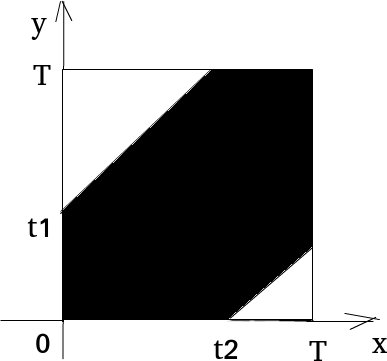
\includegraphics[width=.4\textwidth]{./pictures/4_1.png}
  \caption{Пространство элементарных событий}
  \label{fig:41}
\end{figure}

Множество $A$ точек, которые способствуют встрече, определяется неравенствами
$$A =
\left\{ \left( x, y \right):
0 \leq x \leq y \leq \min \left( T, x + \tau_1 \right),
0 \leq x \leq y \leq \min \left( T, x + \tau_2 \right) \right\}.$$

Очевидно, что
$$m \left( \Omega \right) =
T^2,
m \left( A \right) =
T^2 - \frac{1}{2} \left[ T - \min \left( T, \tau_1 \right) \right]^2 - \frac{1}{2} \left[ T - \min \left( T, \tau_2 \right) \right]^2.$$

Поэтому согласно с
$$P \left\{ A \right\} =
\frac{ \mu \left( A \right) }{ \mu \left( \Omega \right) }$$
имеем
$$P \left\{ A \right\} =
1 - \frac{1}{2} \left\{ \left[ \max \left( 0, 1 - \frac{ \tau_1}{T} \right) \right]^2 + \left[ \max \left( 0, 1 - \frac{ \tau_2}{T} \right) \right]^2 \right\}.$$

\paragraph*{Игла Бюффона}

\textit{Задание.} Рассмотрим плоскость, разделённую параллельными прямыми, которые находятся на расстоянии $2a$ одна от другой (рис. \ref{fig:42}).
На плоскость наугад бросается игла, которая имеет длину $2l$.
Нужно найти вероятность того, что игла пресечёт хотя бы одну из прямых (в случае $l > a$ игла может пересечь несколько прямых).

\begin{figure}[h!]
  \centering
  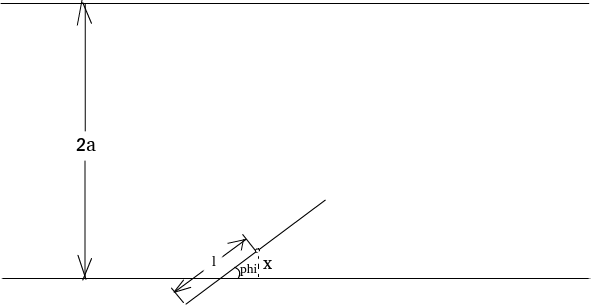
\includegraphics[width=.9\textwidth]{./pictures/4_2.png}
  \caption{Плоскость, разделённая параллельными прямыми}
  \label{fig:42}
\end{figure}

\textit{Решение.}  Положение иглы однозначно определяется расстоянием от центра игла до ближайшей прямой и углом $ \phi $, который образует игла с этой прямой.
Очевидно, что $0 \leq x \leq a$ и $0 \leq \phi \leq \pi $, т.е. пространство элементарных событий $ \Omega $ является прямоугольником (рис. \ref{fig:4201} и \ref{fig:4202}):
$$ \Omega =
\left\{ \left( x, \phi \right):
0 \leq x \leq a,
0 \leq \phi \leq \pi \right\}.$$

Для того, чтобы игла пересекла одну из прямых необходимо и достаточно выполнение условия
$x \leq l \sin \phi$, т.е.
$$A =
\left\{ \left( x, \phi \right):
x \leq l \sin \phi,
0 \leq x \leq a,
0 \leq \phi \leq \pi \right\}.$$

Рассмотрим два случая.

А. $l \leq a$ (рис. \ref{fig:4201}).
Очевидно, что
$$ \mu \left( \Omega \right) =
a \pi,
\mu \left( A \right) =
\int \limits_{0}^{ \pi } l \sin \phi d \phi =
2l,
P \left\{ A \right\} =
\frac{2l}{a \pi}.$$

B. $l > a$ (рис. \ref{fig:4202}).
В этом случае имеем
\begin{equation*}
\begin{split}
\mu \left( A \right) =
a \pi - 2 \int \limits_{0}^{\arcsin \left( \frac{a}{l} \right) } \left( a - l \sin \phi \right) d \phi =
a \left( \pi - 2 \arcsin \frac{a}{l} \right) + \\
+ 2l \left( 1 - \sqrt{1 - \left( \frac{a}{l} \right)^2} \right),
P \left\{ A \right\} =
\frac{ \mu \left( A \right) }{a \pi}.
\end{split}
\end{equation*}

\begin{figure}[h!]
  \centering
  \begin{minipage}[b]{0.4\textwidth}
    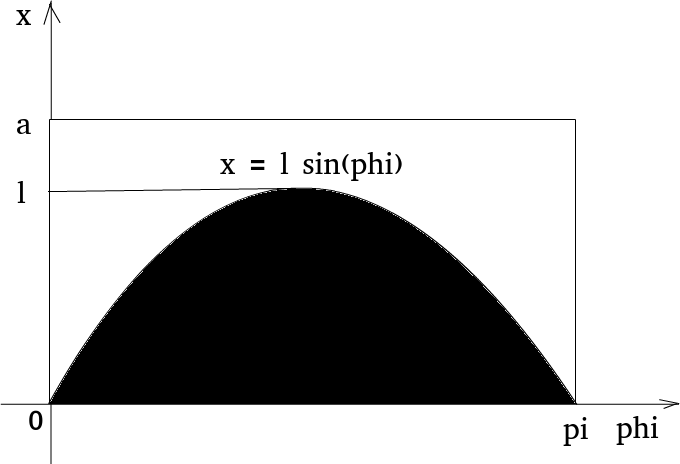
\includegraphics[width=\textwidth]{./pictures/4_201.png}
    \caption{Случай $l \leq a$}
    \label{fig:4201}
  \end{minipage}
  \hfill
  \begin{minipage}[b]{0.4\textwidth}
    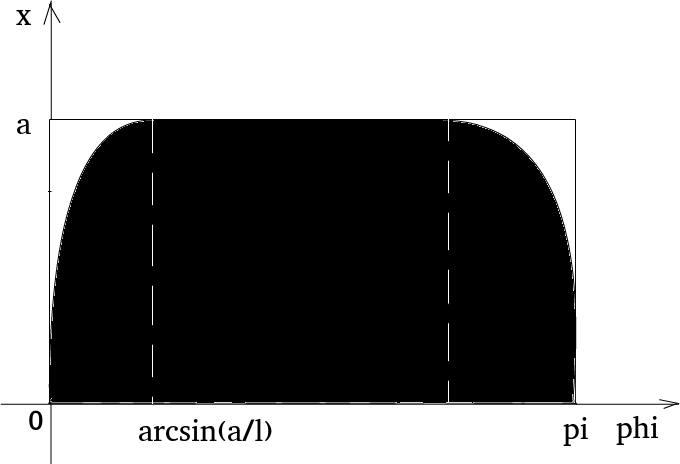
\includegraphics[width=\textwidth]{./pictures/4_202.png}
    \caption{Случай $l > a$}
    \label{fig:4202}
  \end{minipage}
\end{figure}

В случае $l \leq a$ с помощью иглы Бюффона можно приближённо вычислить число $ \pi $.
Действительно, пусть было проведено $n$ экспериментов, в каждом из которых исследовалось пересекла ил игла прямую, или нет.
Обозначим через $ \nu_n$ количество экспериментов, в которых произошло пересечение.
Согласно с усиленным законом больших чисел
$$ \frac{ \nu_n}{n} \xrightarrow[n \rightarrow \infty ]{} P \left\{ A \right\} =
\frac{2l}{a \pi}$$
с вероятностью 1.

Отсюда следует, что
$$ \frac{2l n}{a \nu_n} \xrightarrow[n \rightarrow \infty ]{} \pi $$
с вероятностью 1, т.е. с помощью достаточного количества экспериментов можно вычислить число $ \pi $ с любой точностью.

\addcontentsline{toc}{section}{Аудиторные задачи}
\section*{Аудиторные задачи}

\subsubsection*{4.3}

\textit{Задание.} На отрезке $ \left[ 0, 10 \right] $ числовой оси наугад выбрана точка.
Найдите вероятность того, что расстояние от этой точки до средины отрезка окажется большим чем три.

\textit{Решение.} Обозначим через $x$ расстояние от начала отрезка к точке.
Тогда пространством элементарных событий является отрезок
$ \Omega = \\
= \left\{ x \in \mathbb{R}: \, 0 \leq x \leq 10 \right\} =
\left[ 0, 10 \right] $,
а событию $A$ =
\{расстояние от точки до средины отрезка окажется большим чем 3\}
способствуют точки объединения интервала
$A =
\left\{ x \in \Omega: \, x < 2, \, x > 8 \right\} =
\left[0, 2 \right) \cup \left(8, 10 \right] $.
Поэтому
$$P \left( A \right) =
\frac{|A|}{| \Omega |} =
\frac{4}{10} =
\frac{2}{5}.$$

\subsubsection*{4.4}

\textit{Задание.} В квадрате $ABCD$ со стороной 3 наугад выбрана точка.
Найдите вероятность того, что расстояние от этой точки к:
\begin{enumerate}[label=\alph*)]
\item центру квадрата;
\item стороне $AB$;
\item точке $A$;
\item одной из сторон;
\item диагонали $AC$ не будет превышать 1.
\end{enumerate}

\textit{Решение.} Обозначим через $x$ и $y$ координаты точки.
Пусть точка $A$ имеет координаты $ \left( 0, 0 \right) $,
точка $B$ --- $ \left( 0, 3 \right) $, $C$ --- $ \left( 3, 3 \right) $, и $D$ имеет координаты $ \left( 3, 0 \right) $.
Тогда пространством элементарных событий является квадрат
$ \Omega = \\
=\left\{ \left( x, y \right) \in \mathbb{R}^2: \,
0 \leq x \leq 3,
0 \leq y \leq 3 \right\} $.
Площадь квадрата равна $S_{\Omega} = 3^2 = \\ = 9$.

\begin{enumerate}[label=\alph*)]
\item Центр квадрата --- это точка $ O \left( 3/2, 3/2 \right) $.
Расстояние от точки к центру квадрата не должно превышать единицу --- событие $A$.
Тогда точка должна находиться в круге с радиусом 1 и центром в точке $O$.
Событие описывается множеством
$$A =
\left\{ \left( x, y \right) \in \Omega: \,
\left( \frac{3}{2} - x \right)^2 + \left( \frac{3}{2} - y \right)^2 \leq 1 \right\}.$$

Поэтому
$$P \left( A \right) =
\frac{S_A}{S_{ \Omega }} =
\frac{ \pi \cdot 1^2}{9} =
\frac{ \pi }{9};$$

\item событие $A$ =
\{расстояние от точки к стороне $AB$ не будет превышать единицу\}
описывается множеством $A = \left\{ \left( x, y \right) \in \Omega: \, 0 \leq x \leq 1, 0 \leq y \leq 3 \right\} $.
Изобразив $A$ на плоскости, можно убедиться, что точки множества $A$ образуют прямоугольник со сторонами $1$ и $3$.
Поэтому
$$P \left( A \right) =
\frac{S_A}{S_{ \Omega }} =
\frac{1 \cdot 3}{9} =
\frac{1}{3};$$

\item событие $A =$
\{расстояние к точке $A$ не будет превышать единицу\}
описывается множеством $A =\left\{ \left( x, y \right) \in \Omega: \, x^2 + y^2 \leq 1 \right\} $.
Изобразив $A$ на плоскости, можно убедиться, что $A$ является четвертью круга с центром в начале координат и радиусом 1.
Поэтому
$$P \left( A \right) =
\frac{S_A}{S_{ \Omega }}=
\frac{ \frac{1}{4} \cdot \pi 1^2}{9} =
\frac{ \pi }{36};$$

\item событие $A =$
\{расстояние от точки к одной из сторон не превышает единицу\}
описывается множеством
$$A =
\left\{ \left( x, y \right) \in \Omega: \,
0 \leq x \leq 1,
2 \leq x \leq 3,
0 \leq y \leq 1,
2 \leq y \leq 3 \right\}.$$
Изобразив $A$ на плоскости, можно убедиться, что $A$ --- исходный квадрат с вырезанным квадратом со стороной 1.
Поэтому
$$P \left( A \right) =
\frac{S_A}{S_{ \Omega }} =
\frac{3^2 - 1^2}{9} =
\frac{9-1}{9} =
\frac{8}{9};$$

\item событие $A =$
\{расстояние от точки к диагонали $AC$ не превысит единицы\}
описывается множеством $A = \left\{ \left( x, y \right) \in \Omega: \, 0 \leq \left| y - x \right| \leq 1 \right\}$.
Изобразив $A$ на плоскости, можно убедиться,
что $A$ является квадратом без двух прямоугольных равнобедренных треугольников с катетами $3 - \sqrt{2}$.
Поэтому
$$P \left( A \right) =
\frac{S_A}{S_{ \Omega }} =
\frac{3^2 - 2 \cdot \frac{1}{2} \cdot \left( 3 - \sqrt{2} \right)^2}{9} =
\frac{9 - \left( 3 - \sqrt{2} \right)^2}{9}.$$
\end{enumerate}

\subsubsection*{4.5}

\textit{Задание.} Точка $ \left( \xi, \eta \right) $ наугад выбрана в квадрате $ \left[ 0, 1 \right]^2$.
Для фиксированного $z \in \left( 0, 1 \right) $ вычислить вероятность:
\begin{enumerate}[label=\alph*)]
\item $P \left( \left| \xi - \eta \right| < z \right) $;
\item $P \left( \min \left( \xi, \eta \right) < z \right) $;
\item $P \left( \left( \xi + \eta \right)/2 < z \right) $.
\end{enumerate}

\textit{Решение.}
Пространство элементарных событий можно описать следующим образом:
$ \Omega =
\left\{ \left( \xi, \eta \right) \in \left[ 0, 1 \right]^2 \right\} $.
Изобразив $ \Omega $ на плоскости, можно убедиться, что $ \Omega $ является квадратом со стороной 1.

\begin{enumerate}[label=\alph*)]
\item Событие $A$ описывается множеством
$$A =
\left\{ \left( \xi, \eta \right) \in \Omega: \,
\left| \xi - \eta \right| < z,
z \in \left( 0, 1 \right) \right\}.$$
Изобразив $A$ на плоскости,
можно убедиться,
что точки множества $A$ образуют квадрат с двумя вырезанными прямоугольными равнобедренными треугольниками с катетами $1 - z$.

Найдём площадь треугольника:
$$S = \frac{1}{2} \cdot \left( 1-z \right)^2 =
\frac{ \left( 1-z \right)^2}{2}.$$

Тогда вероятность равна
$$P \left( A \right) =
1 - 2 \cdot \frac{ \left( 1-z \right)^2}{2} =
1 - \left( 1-z \right)^2 =
1 - 1 + 2z - z^2 =
z \left( 2-z \right);$$

\item событие
$A =
\left\{ P \left( \min \left( \xi, \eta \right) < z \right) \right\}$
описывается множеством
$A = \\
= \left\{ \left( \xi, \eta \right) \in \Omega: \,
\min \left( \xi, \eta \right) < z, \,
z \in \left( 0, 1 \right) \right\} $.
Изобразив $A$ на плоскости,
можно убедиться, что точки множества $A$ образуют квадрат со сторонами длиной $1$ без квадрата со стороной длиной $1 - z$ (рис. \ref{fig:45}, \ref{fig:451}).

\begin{figure}[h!]
  \centering
  \begin{minipage}[b]{0.4\textwidth}
    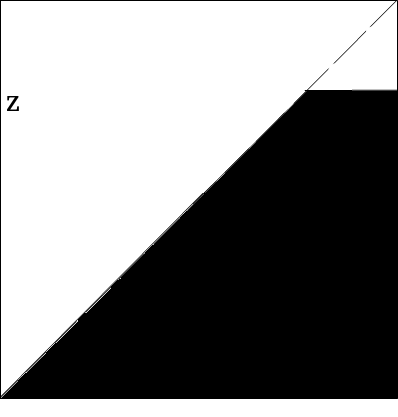
\includegraphics[width=\textwidth]{./pictures/4_5.png}
    \caption{$ \xi < \eta, \min \left( \xi, \eta \right) = \\ = \eta < z$}
    \label{fig:45}
  \end{minipage}
  \hfill
  \begin{minipage}[b]{0.4\textwidth}
    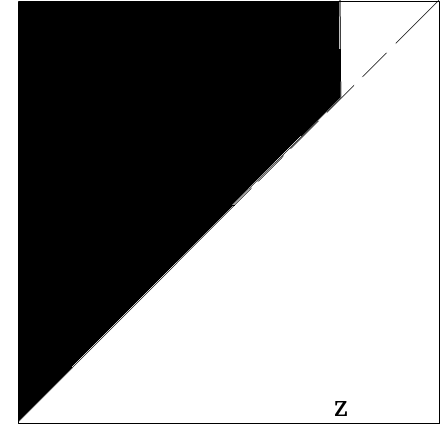
\includegraphics[width=\textwidth]{./pictures/4_5_1.png}
    \caption{$ \xi \geq \eta, \min \left( \xi, \eta \right) = \\ = \xi < z$}
    \label{fig:451}
  \end{minipage}
\end{figure}

Поэтому
$$P =
1 - \left( 1-z \right)^2;$$

\item рассмотрим случай, когда $2z < 1$.
Упростим неравенство. Умножим левую и правую части на $2$.
Получим: $ \xi + \eta < 2z$.
Выразим $ \xi $ и $ \eta: \, \xi < \\ < 2z - \eta, \, \eta < 2z - \xi $.

Событие
$$A =
\left\{ P \left( \frac{ \xi + \eta }{2} < z \right) \right\} $$
описывается множеством
$$A =
\left\{ \left( \xi, \eta \right) \in \Omega: \,
\frac{ \xi + \eta }{2} < z, \,
z \in \left( 0, 1 \right) \right\}.$$
Изобразив $A$ на плоскости, можно убедиться, что точки множества $A$ образуют прямоугольник с катетами $2z$ (рис. \ref{fig:452}).

\begin{figure}[h!]
  \centering
  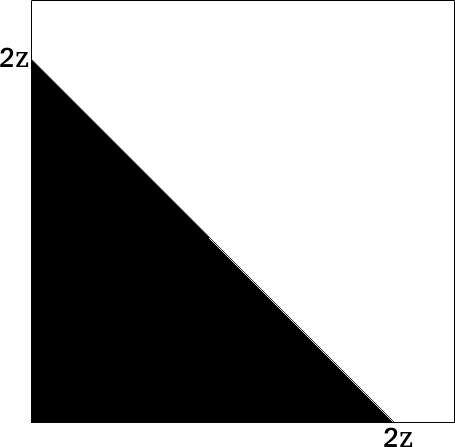
\includegraphics[width=.4\textwidth]{./pictures/4_5_2.png}
  \caption{Точки множества $A, \, 2z < 1$}
  \label{fig:452}
\end{figure}

Поэтому
$$P \left( A \right) =
\frac{S_A}{S_{ \Omega }} =
\frac{ \frac{1}{2} \cdot 2z \cdot 2z}{1 \cdot 1} =
2z^2.$$
\end{enumerate}

Теперь рассмотрим случай, когда $2z > 1$ (рис. \ref{fig:453}).

\begin{figure}[h!]
  \centering
  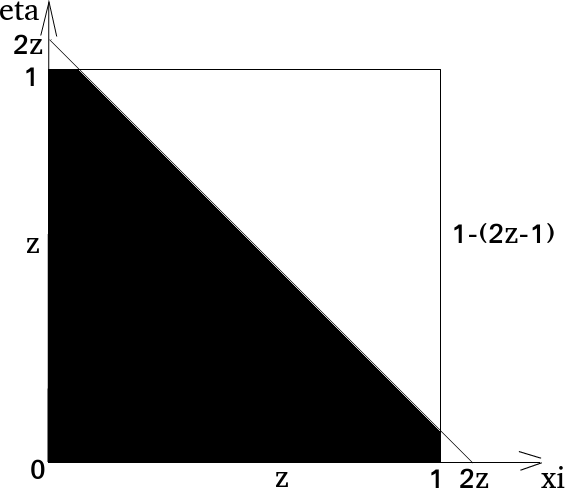
\includegraphics[width=.4\textwidth]{./pictures/4_5_3.png}
  \caption{Точки множества $A, \, 2z > 1$}
  \label{fig:453}
\end{figure}

Вероятность тогда равна
$$P \left( A \right) =
1 - \frac{1}{2} \cdot \left( 2-2z \right)^2 =
1 - 2 \left( 1-z \right)^2.$$

\subsubsection*{4.6}

\textit{Задание.} На отрезке $ \left[ 0, 10 \right] $ числовой оси наугад выбраны две точки.
Найдите вероятность того, что расстояние от правой точки к точке с координатой $8$ окажется меньшим чем единица.

\textit{Решение.} Обозначим через $x$ и $y$ расстояния от начала отрезка (точки $0$) к левой и правой точкам соответственно.
Тогда пространство элементарных событий можно описать следующим образом:
$$ \Omega =
\left\{ \left( x, y \right) \in \mathbb{R}^2: \,
0 \leq x  \leq y \leq 10 \right\},$$
а событие $A =$
\{расстояние от правой точки к точке 8\} описывается множеством $A = \left\{ \left( x, y \right) \in \Omega: \left| \max \left( x, y \right) - 8 \right| < 1 \right\} $.
Изобразив $ \Omega $ и $A$ на плоскости, можно убедиться, что $ \Omega $ является фигурой, изображённой на рис. \ref{fig:46}.

\begin{figure}[h!]
  \centering
  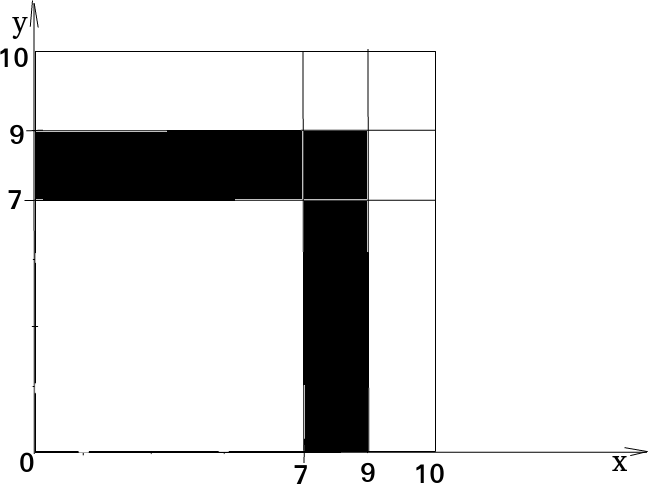
\includegraphics[width=.4\textwidth]{./pictures/4_6.png}
  \caption{Точки множества $A$}
  \label{fig:46}
\end{figure}

Поэтому
$$P \left( A \right) =
\frac{S_A}{S_{ \Omega }} =
\frac{9^2-7^2}{10 \cdot 10} =
\frac{2 \cdot 16}{100} =
\frac{32}{100} =
0.32.$$

\subsubsection*{4.7}

\textit{Задание.} На отрезке $AB$ длиной $a$ наугад выбраны, независимо одна от другой, шесть точек.
Найдите вероятность того, что:
\begin{enumerate}[label=\alph*)]
\item две точки будут находиться от точки $A$ на расстоянии, меньшем чем $b$, а четыре точки --- на расстоянии, большем чем $b \, \left(b<a \right) $;
\item две точки будут находиться от точки $A$ на расстоянии, меньшем чем $c$, одна --- на расстоянии, не меньшем чем $c$ и не большем чем $b$,
и три точки --- на расстоянии, большем чем $b \, \left( c<b<a \right) $.
\end{enumerate}

\textit{Решение.} Обозначим через $x_1, \, x_2, \dotsc, x_6$ расстояния от точки $A$ к выбранным точкам.
Элементарный исход ---  кортеж расстояний от точки $A: \, \omega = <x_1, \, x_2, \dotsc, x_6>$.
Тогда пространство элементарных исходов можно описать следующим образом:
$$ \Omega =
\left\{ <x_1, \, x_2, \dotsc, x_6> \in AB^6:
0 \leq x_1 \leq a, \,
0 \leq x_2 \leq a, \dotsc,
0 \leq x_6 \leq a \right\}.$$

\begin{enumerate}[label=\alph*)]
\item Событие $A =$
\{две точки будут находиться от точки $A$ на расстоянии,
меньшем чем $b$, а четыре точки --- на расстоянии,
большем чем $b \, \left( b<a \right) $\}
описывается множеством
\begin{equation*}
\begin{split}
A = \\
\left\{ <x_1, x_2, \dotsc, x_6> \in \Omega: \,
0 \leq x_1 < b, \,
0 \leq x_2 < b, \,
b < x_3 \leq a, \dotsc,
b < x_6 \leq a \right\}.
\end{split}
\end{equation*}
Возьмём нормированное расстояние $x_i/AB$, чтобы все точки были из $ \left[ 0, 1 \right] $.
Потому $b$ теперь $b/a$.
Событие $A$ примет вид:
$$A =
\left\{ <x_1, \, x_2, \dotsc, x_6> \in \Omega:
x_1 < \frac{b}{a}, \,
x_2 < \frac{b}{a}, \,
x_3 > \frac{b}{a}, \,
x_4 > \frac{b}{a}, \,
x_5 > \frac{b}{a}, \,
x_6 > \frac{b}{a} \right\}.$$

Изобразим двумерный случай (рис. \ref{fig:47}).

\begin{figure}[h!]
  \centering
  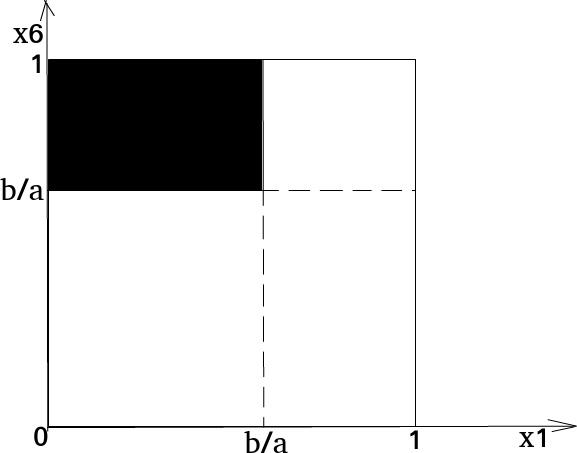
\includegraphics[width=.4\textwidth]{./pictures/4_7.png}
  \caption{Двумерный случай ($x_1$ и $x_6$)}
  \label{fig:47}
\end{figure}

Теперь трёхмерные случаи ($x_1, \, x_2, \, x_6$ и $x_1, \, x_5, \, x_6$) --- рис. \ref{fig:471}.

\begin{figure}[h!]
  \centering
  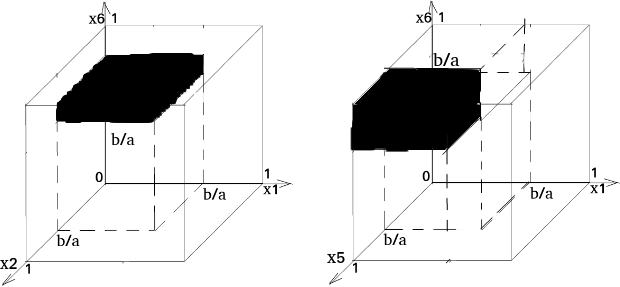
\includegraphics[width=.7\textwidth]{./pictures/4_7_1.png}
  \caption{Трёхмерные случаи}
  \label{fig:471}
\end{figure}

Это параллелепипед со сторонами длиной $b/a$ и $1 - b/a$.
Для 6-мерного случая, его мера равна
$$ \left( \frac{b}{a} \right)^2 \left( 1 - \frac{b}{a} \right)^4.$$
Осталось учесть перестановки, ведь нет разницы, какая точка будет слева: первая или пятая.
Нужно выбрать две точки из шести, которые будут слева от $b/a$.
Посчитали 1 случай, а таких случаев $C_6^2$.
Тогда вероятность равна
$$P =
\frac{C_6^2 \left( \frac{b}{a} \right)^2 \left( 1 - \frac{b}{a} \right)^4}{1^6} =
15 \left( \frac{b}{a} \right)^2 \left( 1 - \frac{b}{a} \right)^4;$$

\item событие $A =$
\{две точки будут находиться от точки $A$ на расстоянии,
меньшем чем $c$ и не большем чем $b$, и три точки ---
на расстоянии, большем чем
$b \,
\left( c<b<a \right)$
описывается множеством
\begin{equation*}
\begin{split}
A = \\
\left\{ <x_1, \, x_2, \dotsc, x_6> \in \Omega: \,
_1 < c, \,
x_2 < c, \,
c \leq x_3 \leq b, \,
b < x_4, \,
b < x_5, \,
b < x_6 \right\}.
\end{split}
\end{equation*}

Возьмём нормированное расстояние $x_i/AB$, чтобы все они были из $ \left[ 0, 1 \right] $.
Потому теперь
\begin{equation*}
\begin{split}
A = \\
\left\{ <x_1, \dotsc, x_6> \in \Omega:
x_1 < \frac{c}{a},
x_2 < \frac{c}{a},
\frac{c}{a} \leq x_3 \leq \frac{b}{a},
\frac{b}{a} < x_4,
\frac{b}{a} < x_5,
\frac{b}{a} < x_6 \right\}.
\end{split}
\end{equation*}

Для 6-мерного случая мера этой фигуры равна
$$ \left( \frac{c}{a} \right)^2 \left( \frac{b}{a} - \frac{c}{a} \right) \left( 1 - \frac{b}{a} \right)^3.$$

Осталось учесть перестановки, ведь нет разницы, какая точка где будет находиться.
Нужно выбрать две точки из шести, которые будут находиться слева от $c/a$ --- это $C_6^2$, а затем одну точку из четырёх, которая будет между $c/a$ и $b/a$ --- $C_4^1$.
Тогда вероятность равна
$$P =
C_6^2 C_4^1 \left( \frac{c}{a} \right)^2 \left( \frac{b}{a} - \frac{c}{a} \right) \left( 1 - \frac{b}{a} \right)^3.$$
\end{enumerate}

\subsubsection*{4.8}

\textit{Задание.} Точку $ \left( \xi, \eta \right) $ выбрано в квадрате $ \left[ 0, 1 \right]^2$.
Найдите вероятность того, что уравнение $x^2 + \xi x + \eta = 0$ имеет:
\begin{enumerate}[label=\alph*)]
\item действительные разные корни;
\item кратные корни.
\end{enumerate}

\textit{Решение.}
Пространство элементарных событий можно описать следующим образом:
$ \Omega =
\left\{ \left( \xi, \eta \right) \in \left[ 0, 1 \right]^2 \right\} $.
Найдём дискриминант квадратного уравнения: $D = \xi^2 - 4 \eta $.

\begin{enumerate}[label=\alph*)]
\item Чтобы уравнение имело 2 разных действительных корня, его дискриминант должен быть больше нуля: $ \xi^2 - 4 \eta > 0$ или $ \xi^2 > 4 \eta $.
Выразив $ \eta $, получим:
$$ \eta < \frac{ \xi^2}{4}.$$
На рисунке \ref{fig:48} эта область изображена голубым цветом.

\begin{figure}[h!]
  \centering
  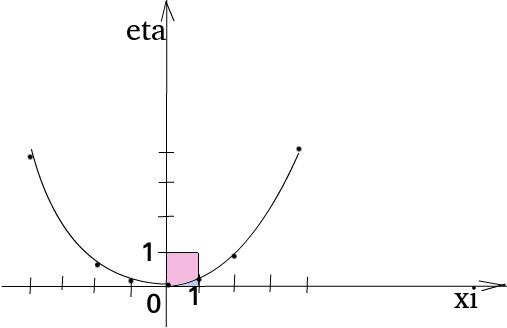
\includegraphics[width=.7\textwidth]{./pictures/4_8.png}
  \caption{$ \eta = \frac{ \xi^2}{4}$}
  \label{fig:48}
\end{figure}

Найдём площадь под кривой:
$$S =
\int \limits_0^1 \frac{ \xi^2}{4}d \xi =
\left. \frac{ \xi^3}{12} \right|_0^1 =
\frac{1}{12}.$$

Тогда вероятность равна
$$P =
\frac{ \frac{1}{12} }{1 \cdot 1} =
\frac{1}{12}.$$

\item чтобы уравнение имело кратные корни, его дискриминант должен быть равен нулю --- эта облась обозначена линией на рисунке.
Плозадь линии равна нулю, поэтому вероятность данного события тоже равна нулю.
\end{enumerate}

\subsubsection*{4.9}

\textit{Задание.} На окружности наугад выбраны три точки $A, \, B$ и $C$.
Найдите вероятность того, что треугольник $ABC$ окажется:
\begin{enumerate}[label=\alph*)]
\item остроугольным;
\item прямоугольным.
\end{enumerate}

\textit{Решение.} Окружность симметрична, поэтому можем выбрать начало отсчёта в точке $A$.
Обозначим через $x$ и $y$ длины дуг от начала отсчёта к точкам $B$ и $C$.
Тогда пространство элементарных событий можно описать следующим образом:
$ \Omega =
\left\{ \left( x, y \right) \in \left[0, 2 \pi \right]^2 \right\}$.
Изобразив $ \Omega $ на плоскости, можно убедиться, что $ \Omega $ является квадратом со стороной $2 \pi$.
Поэтому $S_{ \Omega } = 2 \pi \cdot 2 \pi = 4 \pi^2$.

\begin{enumerate}[label=\alph*)]
\item Событие $A =$
\{треугольник $ABC$ окажется остроугольным\}
описывается множеством
$A =
\left\{ \left( x, y \right) \in \left[ \pi, 2 \pi \right]^2 \right\}$,
т.к. вершины остроугольного треугольника должны находиться по разные стороны от диаметра окружности.
Изобразив $A$ на плоскости, можно убедиться, что точки множества $A$ образуют квадрат со сторонами длиной $ \pi $.
Поэтому $S_A = \pi \cdot \pi = \pi^2$.

Тогда вероятность события $A$ равна
$$P \left( A \right) =
\frac{S_A}{S_{ \Omega }} =
\frac{ \pi^2}{4 \pi^2} =
\frac{1}{4};$$
\item рассмотрим событие $A =$ \{треугольник $ABC$ окажется прямоугольным\}.
Оно описывается множеством
$$A = \left\{ \left( x, y \right) \in \Omega: \, y - x = \pi, x - y = \pi \right\}.$$	
Изобразив $A$ на плоскости, можно убедиться, что точки множества $A$ образуют прямые.
Площадь прямой равна нулю.
Поэтому вероятность события $A$ равна
$P \left( A \right) =
\frac{S_A}{S_{ \Omega }} =
\frac{0}{4 \pi^2} =
0.$
\end{enumerate}

\subsubsection*{4.10}

\textit{Задание.} Две лодки должны подойти к одному причалу.
Появление лодок --- независимые случайные события, равновероятные на протяжении суток.
Найдите вероятность того,
что ни одной из лодок де придётся ждать освобождения причала, если стоянка первой лодки --- один час, а второй --- два часа.

\textit{Решение.} Найдём вероятность того, что лодки <<встретятся>>.
Обозначим моменты появления первой и второй лодок через $x$ и $y$.
Тогда пространство элементарных событий $ \Omega $ имеет вид
(рис. \ref{fig:410}):
$$ \Omega = \left\{ \left( x, y \right): \, 0 \leq x \leq 24, \, 0 \leq y \leq 24 \right\}.$$

\begin{figure}[h!]
  \centering
  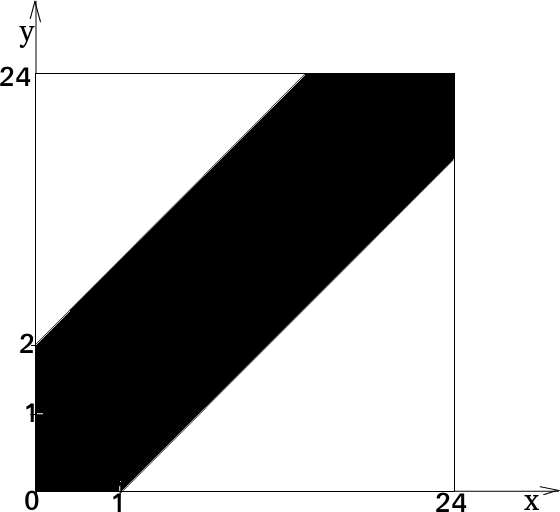
\includegraphics[width=.7\textwidth]{./pictures/4_10.png}
  \caption{Пространство элементарных событий}
  \label{fig:410}
\end{figure}

Множество $A$ точек, которые способствуют встрече, определяется неравенствами
$$A =
\left\{ \left( x, y \right) \in \Omega: \,
0 \leq x \leq y \leq \min \left( 24, x+1 \right), \,
0 \leq x \leq y \leq \min \left( 24, x+2 \right) \right\}.$$

Очевидно, что
\begin{equation*}
\begin{split}
 \mu \left( \Omega \right) = 24^2,
\mu \left( A \right) =
24^2 - \frac{1}{2} \left[ 24 - \min \left( 24, 1 \right) \right]^2 - \frac{1}{2} \left[ 24 - \min \left( 24, 2 \right) \right]^2 = \\
= 24^2 - \frac{1}{2} \left[ 24 - 1 \right]^2 - \frac{1}{2} \left[ 24 - 2 \right]^2 =
24^2 - \frac{1}{2} \cdot 23^2 - \frac{1}{2} \cdot 22^2.
\end{split}
\end{equation*}

Поэтому согласно с
$$P \left\{ A \right\} =
\frac{ \mu \left( A \right) }{ \mu \left( \Omega \right) }$$
имеем
$$P \left\{ A \right\} =
\frac{24^2 - \frac{1}{2} \cdot 23^2 - \frac{1}{2} \cdot 22^2}{24^2} =
1 - \frac{1}{2 \cdot 24^2} \left\{ 23^2 + 22^2 \right\}.$$

Тогда вероятность того, что лодки не <<встретятся>> равна вероятность противоположного события, т.е.
\begin{equation*}
\begin{split}
P \left\{ \overline{A} \right\} =
1 - \left( 1 - \frac{1}{2 \cdot 24^2} \left\{ 23^2 + 22^2 \right\} \right) =
1 - 1 + \frac{1}{2 \cdot 24^2} \left\{ 23^2 + 22^2 \right\} = \\
= \frac{1}{2 \cdot 24^2} \left\{ 23^2 + 22^2 \right\}.
\end{split}
\end{equation*}

\subsubsection*{4.11}

\textit{Задание.}
Путём $ \left\{ S_1, \dotsc, S_x \right\} $
из начала координат в точку
$ \left( x, y \right), \,
x \in \mathbb{N}, \,
y \in \mathbb{Z}$
называется ломаная с вершинами в точках
$ \left( 0, 0 \right), \, \left( 1, S_1 \right), \dotsc, \left( x, S_x \right) $, где $S_x = y, \, S_i - S_{i-1} \in \left\{ -1, 1 \right\} $.
Подсчитайте количество путей:
\begin{enumerate}[label=\alph*)]
\item из $ \left( 0, 0 \right) $ в $ \left( x, y \right) $;
\item из $ \left( 0, 0 \right) $ в $ \left( x, y \right) $, при условии, что $S_1 > 0, \dotsc, S_{x-1} > 0, \, S_x = y > 0$;
\item из $ \left( a, b \right) $ в $ \left( x, y \right) $, которые не пересекают ось абсцисс, при условии, что $a < x, \, x > 0, \, y > 0$.
\end{enumerate}

\textit{Решение.}

\begin{enumerate}[label=\alph*)]
\item Задача изображена на рисунке \ref{fig:411}.

\begin{figure}[h!]
  \centering
  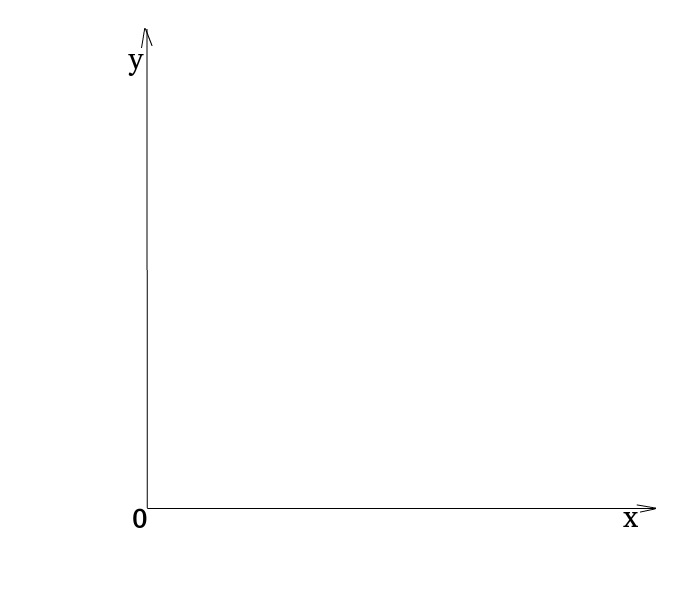
\includegraphics[width=.7\textwidth]{./pictures/4_11.png}
  \caption{Пути из точки $ \left( 0, 0 \right) $ к точке $ \left( x, y \right) $}
  \label{fig:411}
\end{figure}

Переворачиваем изображение --- получаем прямоугольник со сторонами $x'$ и $y'$.
В задании 4.22 уже нашли стороны полученного прямоугольника.
Они равны
$$x' = \frac{x+y}{2}, \, y' = \frac{x-y}{2}.$$

Нужно выбрать шаги, на которых будем перемещаться вверх, тогда на всех остальных шагах остаётся переместиться вправо.
Имеем, что путей из точки $ \left( 0, 0 \right) $ в точку $ \left( x', y' \right) $ всего
$$C_{ \frac{x+y}{2} + \frac{x-y}{2} }^{ \frac{x+y}{2} } =
C_{x}^{ \frac{x+y}{2} } =
\frac{x!}{ \left( \frac{x+y}{2} \right)! \left( x - \frac{x+y}{2} \right)!} =
\frac{x!}{ \left( \frac{x+y}{2} \right)! \left( \frac{x-y}{2} \right)!};$$

\item если путь касается оси абсцисс, его можно отразить.
Тогда количество нужных путей --- разница путей от точки $ \left( 1, 1 \right) $ в точку $ \left( x, y \right) $ и путей из точки $ \left( 0, 0 \right) $ в точку с координатами $ \left( x, -y \right) $.
Для перевёрнутого треугольника --- разница путей из точки
$$ \left( \frac{1+1}{2}, \frac{1-1}{2} \right) =
\left( 1, 0 \right) $$
в точку
$$ \left( \frac{x+y}{2}, \frac{x-y}{2} \right) $$
и путей из точки $ \left( 1, 0 \right) $ в точку
$$ \left( \frac{x-y}{2}, \frac{x+y}{2} \right).$$

Всего путей
$$C_{ \frac{x+y}{2} - 1 + \frac{x-y}{2} }^{ \frac{x-y}{2} } =
C_{x-1}^{ \frac{x+y}{2} } =
\frac{ \left( x-1 \right)!}{ \left( \frac{x-y}{2} \right)! \left( x - 1 - \frac{x-y}{2} \right)!} =
\frac{ \left( x-1 \right)!}{ \left( \frac{x-y}{2} \right)! \left( \frac{x+y}{2} - 1 \right)!}.$$

Путей, которые касаются или пересекают диагональ
$$C_{ \frac{x-y}{2} - 1 + \frac{x+y}{2}}^{ \frac{x+y}{2} } =
C_{x-1}^{ \frac{x+y}{2} } =
\frac{ \left( x-1 \right)!}{ \left( x - 1 - \frac{x+y}{2} \right)! \left( \frac{x+y}{2} \right)!} =
\frac{ \left( x-1 \right)!}{ \left( \frac{x-y}{2} - 1 \right)! \left( \frac{x+y}{2} \right)!}.$$

Тогда количество необходимых путей равно
\begin{equation*}
\begin{split}
\frac{ \left( x-1 \right)!}{ \left( \frac{x-y}{2} \right)! \left( \frac{x+y}{2} - 1 \right)!} -
\frac{ \left( x-1 \right)!}{ \left( \frac{x-y}{2} - 1 \right)! \left( \frac{x+y}{2} \right)!} = \\
= \left( x-1 \right)! \cdot
\left( \frac{1}{ \left( \frac{x-y}{2} -1 \right)! \frac{x-y}{2} \left( \frac{x+y}{2} - 1 \right)!} -
\frac{1}{ \left( \frac{x-y}{2} - 1 \right)! \left( \frac{x+y}{2} - 1 \right)! \frac{x+y}{2} } \right) = \\
= \frac{ \left( x-1 \right)!}{ \left( \frac{x-y}{2} -1 \right)! \left( \frac{x+1}{2} -1 \right)! } \cdot
\left( \frac{1}{ \frac{x-y}{2}} - \frac{1}{ \frac{x+y}{2} } \right) = \\
= \frac{ \left( x-1 \right)!}{ \left( \frac{x-y}{2} -1 \right)! \left( \frac{x+1}{2} -1 \right)! } \cdot
\left( \frac{2}{x-y} - \frac{2}{x+y} \right) = \\
= \frac{ \left( x-1 \right)!}{ \left( \frac{x-y}{2} -1 \right)! \left( \frac{x+1}{2} -1 \right)! } \cdot
\frac{2 \left( x+y \right) - 2 \left( x-y \right) }{ \left( x-y \right) \left( x+y \right) } = \\
= \frac{ \left( x-1 \right)!}{ \left( \frac{x-y}{2} -1 \right)! \left( \frac{x+1}{2} -1 \right)! } \cdot
\frac{4y}{ \left( x-y \right) \left( x+y \right) } = \\
= \frac{ \left( x-1 \right)!}{ \left( \frac{x-y}{2} -1 \right)! \left( \frac{x+1}{2} -1 \right)! } \cdot
\frac{y}{ \frac{x-y}{2} \cdot \frac{x+y}{2} } =
\frac{ \left( x-1 \right)! y}{ \left( \frac{x-y}{2} \right)! \left( \frac{x+y}{2} \right)!};
\end{split}
\end{equation*}
\item чтобы путь не пересекал оси абсцисс, $b$ должно быть больше нуля.
Сведём задачу к предыдущей, отняв от координаты $x$ координату $a$,
а от координаты $y$ --- координату $b$, тем самым переместив точку $ \left( a, b \right) $ в начало координат.
Теперь имеем прямоугольник со сторонами 
$$x' = \frac{x-a+y-b}{2}, y' = \frac{x-a-y+b}{2}.$$

Всего путей
$$C_{ \frac{x-a+y-b}{2} - 1 + \frac{x-a-y+b}{2} }^{ \frac{x-a-y+b}{2} } =
C_{x-a-1}^{ \frac{x-a-y+b}{2} }.$$

Путей, которые касаются или пересекают диагональ
$$C_{ \frac{x-a-y+b}{2} - 1 + \frac{x-a+y-b}{2}}^{ \frac{x-a+y-b}{2} } =
C_{x-a-1}^{ \frac{x-a+y-b}{2} }.$$

Тогда количество необходимых путей равно
$$C_{x-a-1}^{ \frac{x-a-y+b}{2} } - C_{x-a-1}^{ \frac{x-a+y-b}{2} }.$$
\end{enumerate}

\subsubsection*{4.12}

\textit{Задание.} В буфете продаются пирожки стоимостью 50 коп.
Около буфета собралось $m+n$ студентов,
причём $n$ из них имеют монеты по $50$ коп., а остальные $m$ имеют только по одной гривне $ \left( m \leq n \right) $.
Найдите вероятность того, что ни одному студенту не придётся ждать сдачи, если в начале работы в кассе не было денег.

\textit{Решение.} Первым должен стоять тот, который имеет 50 коп.
Должно быть $n$ шагов вверх, $m$ шагов вправо, причём $m < n$ (рис. \ref{fig:412}).

\begin{figure}[h!]
  \centering
  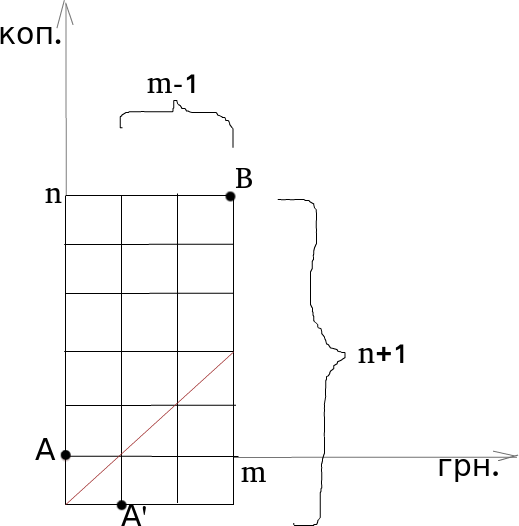
\includegraphics[width=.5\textwidth]{./pictures/4_12.png}
  \caption{Возможные пути}
  \label{fig:412}
\end{figure}

Красной линией на рисунке обозначена линия, которой мы не должны касаться.
Количество таких путей равно
$ \left| \widetilde{A \rightarrow B} \right| =
\left| A \rightarrow B \right| - \\
- \left| A' \rightarrow B \right| =
C_{n+m}^n - C_{n+m}^{n+1}$.

Событие $D =$ \{ни одному студенту не придётся ждать сдачи\}.
Его мощность равна $ \left| D \right| = C_{n+m}^n - C_{n+m}^{n+1}$.
Вероятностное пространство: $ \Omega =$ \{все пути из $A$ в $B$\}.
Оно содержит $ \left| \Omega \right| = C_{n+m}^n$ элементов.
Тогда вероятность равна
$$P \left( D \right) =
\frac{ \left| D \right| }{ \left| \Omega \right| } =
\frac{C_{n+m}^n - C_{n+m}^{n+1}}{C_{n+m}^n} =
1 - \frac{C_{n+m}^{n+1}}{C_{n+m}^n} =
1 - \frac{m}{n+1}.$$

\addcontentsline{toc}{section}{Дополнительные задачи}
\section*{Дополнительные задачи}

\subsubsection*{4.13}

\textit{Задание.} В квадрате наугад выбраны две точки $A$ и $B$.
Найдите вероятность того, что круг, диаметром которого есть отрезок $AB$, полностью будет содержаться в данном квадрате.

\textit{Решение.} Пусть сторона квадрата равна $a$.

Опишем пространство элементарных событий
$$ \Omega =
\left\{ < \left( x_A, y_A \right), \left( x_B, y_B \right) > \in \left[ 0, a \right]^2 \right\}.$$
Изобразив $ \Omega $ на плоскости, можно убедиться, что это квадрат со стороной $a$.

Если в квадрате нарисовать вписанный круг, то обе точки должны лежать внутри этого круга.
Вероятность попадания первой точки в этот круг можно выразить соотношением площадей круга и квадрата,
вероятность дважды попасть в этот круг есть произведение этих вероятностей (соотношений).

$$P \left( A \right) =
\frac{S_A}{S_{ \Omega }} =
\frac{ \left( \pi \cdot \left( \frac{a}{2} \right)^2 \right)^2}{ \left( a^2 \right)^2} =
\frac{ \pi^2 a^4}{4a^4} =
\frac{ \pi }{4}.$$

\subsubsection*{4.14}

\textit{Задание.}
Две частицы независимо друг от друга совершают случайное блуждание на $ \mathbb{Z} $,
причём каждая из них за один шаг передвигается на единицу вправо или влево с вероятностями $1/2$.
В начальный момент времени частицы находятся на расстоянии $2m$ друг от друга.
Каждая из частиц сделала $n$ шагов.
Найдите вероятность того, что частицы впервые встретятся на $n$-м шаге.

\textit{Решение.} Пусть есть одна точка, которая находится в нуле.
Тогда определить, в какой точке она находится после $n$ шагов, можно, отняв от количества шагов вправо количество шагов влево.
Путей есть $2^n$.
Нужно почитать количества возможных путей длиной $n$, где разность между количеством шагов вправо и количеством шагов влево равна $t$.
Найдём, сколько шагов вправо в таком случае нужно сделать:
$$right - left = t; \, right + left = n \rightarrow right = \frac{t+n}{2}.$$
Тогда количество путей равно $C_n^{ \frac{t+n}{2} }$.

Когда $n < m$, путей не существует, поэтому вероятность равна нулю.

Количество шагов вправо от второй точки до точки $t$ равно $t - 2m$.
Тогда количество путей из второй точки к точке $t$ равно $C_n^{ \left| t-2m \right| }$.

Количество пар путей, при которых две точки встретятся в точке $t$ при отсчёте от левой точки равно $C_n^{ \frac{t+n}{2} } C_n^{ \left| t-2m \right| }$.
Правая точка может максимально уйти в точку $2m - n$ влево --- это минимум $t$.
Максимальная точка, в которую обе могут прийти --- это максимум $t$.
Она равна $n$.
Количество всех путей при всех возможных $t$ равно $ \sum \limits_{t=2m-n}^n C_n^{ \frac{t+n}{2} } C_n^{ \left| t-2m \right| }$.

Количество всех путей равно $2^n \cdot 2^n$.
Тогда вероятность равна
$$P \left( A \right) =
\frac{ \sum \limits_{t=2m-n}^n C_n^{ \frac{t+n}{2} } C_n^{ \left| t-2m \right| }}{2^n \cdot 2^n}.$$

\addcontentsline{toc}{section}{Домашнее задание}
\section*{Домашнее задание}

\subsubsection*{4.15}

\textit{Задание.} На отрезке $AB$ длиной $l$ наугад выбрана точка $O$.
Найдите вероятность того, что отношение $|AO|:|AB|$ не превышает $0.6$.

\textit{Решение.} Обозначим через $x$ расстояние от точки $A$ до точки $O$.
Тогда пространством элементарных событий является отрезок
$ \Omega = \\
= \left\{ x \in \mathbb{R}: 0 \leq x \leq l \right\} =
\left[ 0, l \right] $,
а событию $B = $ 
\{отношение $|AO|:|AB|$ окажется не большим чем $0.6$\}
способствуют точки отрезка
$$B =
\left\{ x \in \Omega : \frac{x}{l} \leq 0.6 \right\} =
\left\{ x \in \left[ 0, l \right] : x \leq 0.6 l \right\} =
\left[ 0, 0.6 l \right].$$
Поэтому
$$P \left( B \right) =
\frac{|B|}{| \Omega |} =
\frac{0.6 l}{l} =
0.6.$$

\subsubsection*{4.16}

\textit{Задание.} На отрезке $ \left[ -1, 2 \right] $ наугад выбрано две точки $A$ и $B$.
Найдите вероятность того, что расстояние между ними окажется меньшим чем $2$, и точка $A$ будет лежать левее единицы.

\textit{Решение.} Обозначим через $x$ и $y$ расстояния от начала отрезка к соответственно точкам $A$ и $B$.
Тогда пространство элементарных событий можно описать следующим образом:
$ \Omega =
\left\{ \left( x, y \right) \in \mathbb{R}^2: -1 \leq x \leq 2, \, -1 \leq y \leq 2 \right\}$,
а событие $A = $ \{расстояние между точками $A$ и $B$ окажется меньшим чем $2$, и точка $A$ будет лежать левее единицы\}
описывается множеством $A = \left\{ \left( x, y \right) \in \Omega: -1 \leq x < 1, y - x < 2, y \leq 2 \right\}$.
Изобразив $ \Omega $ и $A$ на плоскости, можно убедиться, что $ \Omega $ является квадратом со стороной $3$,
а точки множества $A$ образуют прямоугольник со сторонами длиной 2 и 3 с вырезанным треугольником с катетами длиной $1$.
Поэтому
$$P \left( A \right) =
\frac{S_A}{S_{ \Omega }} =
\frac{2 \cdot 3 - \frac{1}{2} \cdot 1 \cdot 1}{3 \cdot 3} =
\frac{11}{18}.$$

\subsubsection*{4.17}

\textit{Задание.} Точка $ \left( \xi, \eta \right) $ наугад выбрана в квадрате $ \left[ 0, 1 \right]^2$.
Для фиксированного $z \in \left( 0, 1 \right) $ вычислить вероятности:
\begin{enumerate}[label=\alph*)]
\item $P \left( \xi + 2 \eta < z \right) $;
\item $P \left( \max \left( \xi, \eta \right) < z \right) $;
\item $P \left( \xi \eta < z \right) $.
\end{enumerate}

\textit{Решение.} Пространство элементарных событий можно описать следующим образом:
$ \Omega =
\left\{ \left( \xi, \eta \right) \in \left[ 0, 1 \right]^2 \right\}$.
Изобразив $ \Omega $ на плоскости, можно убедиться, что $ \Omega $ является квадратом со стороной 1.

\begin{enumerate}[label=\alph*)]
\item Событие $A$ описывается множеством
$A =
\left\{ \left( \xi, \eta \right) \in \Omega:
\xi + 2 \eta < z, z \in \left( 0, 1 \right) \right\}$.
Изобразив $A$ на плоскости, можно убедиться,
что точки множества $A$ образуют прямоугольный треугольник с катетами от $0, 0$ до $1/2, 1$ в зависимости от $z$.

Выразим длины катетов через $z$.
При $ \xi = 0$ получаем, что
$$ \eta < \frac{z}{2}.$$
При $ \eta = 0$ получаем, что $ \xi < z$.
Поэтому верхняя грань одного из катетов равна $z$, а второго --- $z/2$.
Найдём площадь треугольника:
$$S_A =
\frac{1}{2} \cdot z \cdot \frac{z}{2} =
\frac{z^2}{4}.$$

Тогда вероятность равна
$$P \left( A \right) =
\frac{S_A}{S_{ \Omega }} =
\frac{ \frac{z^2}{4} }{1} =
\frac{z^2}{4}.$$

Найдём вероятности данного события при верхней и нижней гранях $z$ (при $z=0$ и $z=1$).

При $z=0$ точки множества $A$ образуют прямоугольный треугольник с катетом, равным нулю.
Поэтому
$$P \left( A \right) =
\frac{S_A}{S_{ \Omega }} =
\frac{0}{1 \cdot 1} =
0.$$

При $z=1$ точки множества $A$ образуют прямоугольный треугольник с катетами, равными $1/2$ и $1$.
Поэтому
$$P \left( A \right) =
\frac{ \frac{1}{2} \cdot \frac{1}{2} \cdot 1}{1 \cdot 1} =
\frac{1}{4}.$$

Отсюда следует, что вероятность данного события лежит в пределах
$$P \left( A \right) \in \left( 0, \frac{1}{4} \right).$$

Пусть $ \Omega $ представляет собой куб со стороной $1$;

\item рассмотрим вариант, когда $ \eta > \xi $.
Тогда $ \max \left( \xi, \eta \right) = \eta < z$.
При $ \eta \leq \xi $ получаем, что $ \max \left( \xi, \eta \right) = \xi < z$.
Прямая $ \eta = \xi $ делит квадрат на 2 одинаковых треугольника.
Пусть $z = 1/2$.
Если $ \xi \geq \eta $, то $ \xi < z$.
Поэтому точка может лежать в нижнем треугольнике левее от вертикальной прямой $ \xi = 1/2$.
Аналогично при $ \eta > \xi : \, \eta < z$ --- точка может лежать в верхнем треугольнике ниже горизонтальной прямой $ \eta = 1/2$.
Объединив эти 2 случая имеем, что точка может попасть в квадрат со стороной $z$.
Тогда вероятность равна
$$P \left( A \right) =
\frac{S_A}{S_{ \Omega }} =
\frac{z \cdot z}{1} =
z^2;$$

\item найдём площадь фигуры с помощью интеграла.
Разобьём её площадь на две фигуры: на прямоугольник со сторонами $1$ и $z$ и на фигуру, ограниченную прямыми $ \xi = z, \, \xi = 1$ и кривой
$$ \eta =
\frac{z}{ \xi }.$$
Площадь прямоугольника равна $S_{A_1} = 1 \cdot z = z$.
Площадь фигуры под кривой найдём с помощью интеграла.
Она будет равна
$$S_{A_2} =
\int \limits_{z}^1 \frac{z}{ \xi } d \xi =
\left. z \cdot \ln \xi \right|_z^1 =
z \left( - \ln z + \ln 1 \right) =
z \ln z.$$

Тогда площадь фигуры равна $S_A = S_{A_1} + S_{A_2} = z - z \ln z = z \left( 1 - \ln z \right)$.

Вероятность равна
$$P \left( A \right) =
\frac{S_A}{S_{ \Omega }} =
\frac{z \left( 1 - \ln z \right) }{1} =
z \left( 1 - \ln z \right).$$
\end{enumerate}

\subsubsection*{4.18}

\textit{Задание.} На окружности выбраны три точки $A, \, B$ и $C$.
Найдите вероятность того, что треугольник $ABC$ окажется:
\begin{enumerate}[label=\alph*)]
\item тупоугольным;
\item равнобедренным.
\end{enumerate}

\textit{Решение.} Окружность симметрична, поэтому можем выбрать начало отсчёта в точке $A$.
Обозначим через $x$ и $y$ длины дуг от начала отсчёта к точкам $B$ и $C$.
Тогда пространство элементарных событий можно описать следующим образом:
$ \Omega =
\left\{  \left( x, y \right) \in \left[0, 2 \pi \right]^2 \right\}$.
Изобразив $ \Omega $ на плоскости, можно убедиться, что $ \Omega $ является квадратом со стороной $2 \pi$.
Поэтому $S_{ \Omega } = 2 \pi \cdot 2 \pi = 4 \pi^2$.

\begin{enumerate}[label=\alph*)]
\item Событие $А = $ \{1 из углов треугольника $ABC$ окажется тупоугольным\} описывается множеством
$A =
\left\{ \left( x, y \right) \in \left[0, \pi \right]^2 \right\}$,
т.к. вершины тупоугольного треугольника должны находиться по одну сторону от диаметра окружности.
Изобразив $A$ на плоскости, можно убедиться, что точки множества $A$ образуют квадрат со стороной $ \pi $.
Поэтому $S_A = \\ = \pi \cdot \pi = \pi^2$.

Так как тупым может быть любой из трёх углов треугольника,
то событие $S_B = 3S_a = 3 \pi^2$, где $B =$ \{треугольник $ABC$ окажется тупоугольным\}.

Тогда вероятность события $B$ равна
$$P \left( B \right) =
\frac{S_B}{S_{ \Omega }} =
\frac{3 \pi^2}{4 \pi^2} =
\frac{3}{4};$$

\item рассмотрим событие $A = $ \{треугольник $ABC$ окажется равнобедренным\}.
Оно описывается множеством 
$$A = \left\{ \left( x, y \right) \in \left[0, 2 \pi \right]^2: x = y, y = 2 \pi - x, y = 2x, x = 2y \right\}.$$
Изобразив $A$ на плоскости, можно убедиться, что точки множества $A$ образуют прямые.
Площадь прямой равна нулю.
Поэтому вероятность события $A$ равна
$$P \left( A \right) =
\frac{0}{4 \pi^2} =
0.$$
\end{enumerate}

\subsubsection*{4.19}

\textit{Задание.} Карандаш длиной $l$ разломано наугад на три части.
Найдите вероятность того, что длина средней части окажется самой меньшей.

\textit{Решение.} Обозначим через $x$ и $y$ расстояния от кончика карандаша до соответственно ближней к нему и дальней от него точек разлома.
Тогда пространство элементарных событий можно описать следующим образом:
$$ \Omega =
\left\{ \left( x, y \right) \in \mathbb{R}^2:
0 \leq x \leq y \leq l \right\},$$
а событие $A =$
\{длина средней части окажется самой меньшей\} описывается множеством $A = \left\{ \left( x, y \right) \in \Omega: y - x < x, y - x < l - y \right\} $ или
$$A =
\left\{ \left( x, y \right) \in \Omega:
y < 2x,
x > 2y - l \right\}.$$ 
Изобразив $ \Omega $ и $A$ на плоскости,
можно убедиться,
что $ \Omega $ является прямоугольным треугольником с катетами длиной $l$,
а точки множества $A$ образуют треугольник, который лежит между прямыми $y = 2x, y = x$ и $y = \left( x+l \right) /2$.
Найдём координаты вершин треугольника.
Решим уравнение
$$2x = \frac{x+l}{2}.$$
Получим
$$x = \frac{l}{3}, y = \frac{2l}{3}.$$
Две другие вершины имеют координаты $ \left( 0, 0 \right), \left( l, l \right)$.
Найдём площадь треугольника с помощью интеграла.
Разобьём его на две части вертикальной прямой $x = l/3$.
Площадь левого кусочка равна 
$$S_1 =
\int \limits_{0}^{ \frac{l}{3} } 2 x dx =
\left. \frac{2x^2}{2} \right|_0^{ \frac{l}{3} } =
\left. x^2 \right|_0^{ \frac{l}{3} } =
\frac{l^2}{9}.$$
Найдём площадь правого кусочка:
\begin{equation*}
\begin{split}
S_2 =
\int \limits_{ \frac{l}{3} }^l \frac{1}{2} \left( x+l \right) dx =
\frac{1}{2} \left( \int \limits_{ \frac{l}{3} }^l x dx + \int \limits_{ \frac{l}{3} }^l l dx \right) =
\frac{1}{2} \left( \left. \frac{x^2}{2} \right|_{ \frac{l}{3} }^l + \left. lx \right|_{ \frac{l}{3} }^l \right) = \\
= \frac{1}{2} \left( \frac{l^2}{2} - \frac{l^2}{18} + l^2 - \frac{l^2}{3} \right) =
\frac{l^2}{2} \left( \frac{1}{2} - \frac{1}{18} + 1 - \frac{1}{3} \right) =
\frac{l^2}{2} \cdot \frac{9-1+18-6}{18} = \\
= \frac{20 l^2}{2 \cdot 18} =
\frac{10 l^2}{18} =
\frac{5 l^2}{9}.
\end{split}
\end{equation*}

Сложим две площади:
$$S =
S_1 + S_2 = 
\frac{l^2}{9} + \frac{5 l^2}{9} =
\frac{6 l^2}{9} =
\frac{2 l^2}{3}.$$
Теперь отнимем площадь прямоугольного треугольника с катетами длиной $l$.
Получим:
$$S_A =
\frac{2 l^2}{3} - \frac{1}{2} \cdot l \cdot l =
\frac{2 l^2}{3} - \frac{l^2}{2} =
\frac{l^2}{6}.$$

Поэтому
$$P \left( A \right) =
\frac{S_A}{S_{ \Omega }} =
\frac{ \frac{l^2}{6} }{ \frac{l^2}{2} } =
\frac{1}{3}.$$

\subsubsection*{4.20}

\textit{Задание.} На паркет наугад брошена монета радиусом $1$ см.
Найдите вероятность того, что монета не пересечёт сторон паркета, если паркет имеет форму прямоугольников со сторонами $4$ см и $8$ см.

\textit{Решение.} Положение монеты однозначно определяется расстояниями $x$ и $y$ от центра монеты к сторонам ближайшего прямоугольника.
Очевидно, что $0 \leq x \leq 2$ и $0 \leq y \leq 4$, т.е. пространство элементарных событий $ \Omega $ является прямоугольником (рис. \ref{fig:420}):
$ \Omega =
\left\{ \left( x, y \right): 0 \leq x \leq 2, \, 0 \leq y \leq 4 \right\}$.

\begin{figure}[h!]
  \centering
  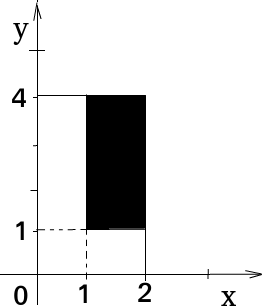
\includegraphics[width=.5\textwidth]{./pictures/4_20.png}
  \caption{Пространство элементарных событий $ \Omega $ и событие $A$}
  \label{fig:420}
\end{figure}

Для того,
чтобы монета не пересекла ни одной из сторон паркета необходимо и достаточно выполнения условий
$1 \leq x \leq 2, \, 1 \leq y \leq 4$, т.е. $A = \left\{ \left( x, y \right): \, 1 \leq x \leq 2, \, 1 \leq y \leq 4 \right\} $.

Имеем
$$P \left\{ A \right\} =
\frac{S_A}{S_{ \Omega }} =
\frac{1 \cdot 3}{2 \cdot 4} =
\frac{3}{8}.$$

\subsubsection*{4.21}

\textit{Задание.} На окружности радиуса $r$ наугад выбраны две точки.
Найдите вероятность того, что расстояние между ними не превышает $r$.

\textit{Решение.} На окружности наугад выбраны две точки $A$ и $B$. Изобразим окружность на рис. \ref{fig:421}.

\begin{figure}[h!]
  \centering
  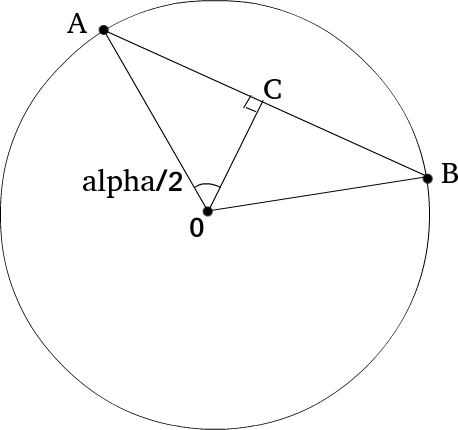
\includegraphics[width=.6\textwidth]{./pictures/4_21.png}
  \caption{Окружность радиуса $r$}
  \label{fig:421}
\end{figure}

Имеем равнобедренный треугольник $AOB$.
Известен размер боковых сторон треугольника и угол $ \alpha $ между ними.
Пусть элементарные исходы --- это углы $ \alpha $.
Угол однозначно опишет эту систему.
Если поделить напополам этот треугольник, получим 2 прямоугольных треугольника с гипотенузами $r$.
Угол между гипотенузой и высотой равен $ \alpha/2$.
Отношение противоположного катета к гипотенузе --- это
$$ \sin \frac{ \alpha }{2} =
\frac{AC}{AO} =
\frac{AC}{r}.$$
Нужно, чтобы катет $AC$ варьировался в пределах
$$ \left[ - \frac{r}{2}, \frac{r}{2} \right].$$
Значит
$$ \sin \frac{ \alpha }{2} \in \left[ - \frac{1}{2}, \frac{1}{2} \right].$$
Это соответствует углам
$$ \frac{ \alpha }{2} \in \left[ -30 \degree, 30 \degree \right].$$
Для угла $ \alpha $ --- это $ \left[ -60 \degree, 60 \degree \right].$
Имеем, что
$ \Omega =
\left\{ \alpha \in \left[ -180 \degree, 180 \degree \right] \right\}, \,
\left| \Omega \right| = \\
= 360 \degree, \,
A =
\left\{ \alpha \in \left[ -60 \degree, 60 \degree \right] \right\}, \,
\left| A \right| =
120 \degree $.
Поэтому вероятность события $A$ равна
$$P \left( A \right) =
\frac{ \left| A \right| }{ \left| \Omega \right| } =
\frac{120}{360} =
\frac{1}{3}.$$

\subsubsection*{4.22}

\textit{Задание.} Подсчитайте количество путей:
\begin{enumerate}[label=\alph*)]
\item из $ \left( 0, 0 \right) $ в $ \left( 2n, 0 \right) $ таких, что:
\begin{enumerate}[label=(\roman*)]
\item $S_1 > 0, \dotsc, S_{2n-1} > 0$;
\item $S_1 \geq 0, \dotsc, S_{2n-1} \geq 0$;
\end{enumerate}

\item из $ \left( 0, m \right) $ в $ \left( n, 0 \right) $, таких, что:
\begin{enumerate}[label=(\roman*)]
\item $S_1 > 0, \dotsc, S_{2n-1} > 0$;
\item $S_1 \geq 0, \dotsc, S_{2n-1} \geq 0$.
\end{enumerate}
\end{enumerate}

\textit{Решение.} Путём $ \left\{ S_1, \dotsc, S_x \right\} $ из начала координат в точку
$ \left( x, y \right), \, x \in \\ \in \mathbb{N}, \, y \in \mathbb{N} $
называется ломаная с вершинами в точках
$ \left( 0, 0 \right), \, \left( 1, S_1 \right), \\ \left( 2, S_2 \right), \dotsc, \left( x, S_x \right) $, где $S_x = y, \, S_i - S_{i-1} \in \left\{ -1, 1 \right\} .$

\begin{enumerate}[label=\alph*)]
\item Сведём задачу к задаче, которая решается с помощью метода отражений.
Введём новую систему координат, которая повёрнута относительно данной на $45 \degree $ по часовой стрелке.
В этой системе координат за 1 шаг будет изменяться две координаты (рис. \ref{fig:422}).

\begin{figure}[h!]
  \centering
  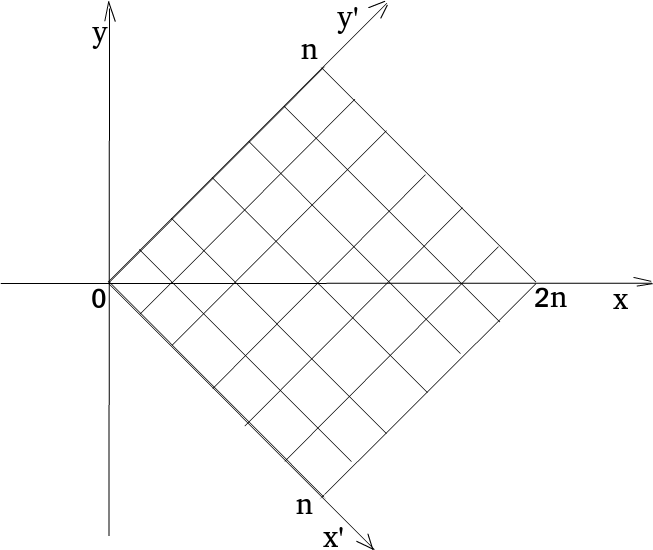
\includegraphics[width=.7\textwidth]{./pictures/4_22.png}
  \caption{Новая система координат}
  \label{fig:422}
\end{figure}

Свели данную задачу к задаче $1.22$.
Имеем пути, состоящие из $n + n$ ходов, среди которых ровно $n$ ходов в направлении $x'$, и $n$ ходов в направлении $y'$.
Если выберем, на каких шагах увеличиваем первую координату, будем знать, где увеличиваем вторую координату.
Это будет $C_{2n}^n$.

\begin{enumerate}[label=(\roman*)]
\item Развернём для удобства рисунок (рис. \ref{fig:4221}).

\begin{figure}[h!]
  \centering
  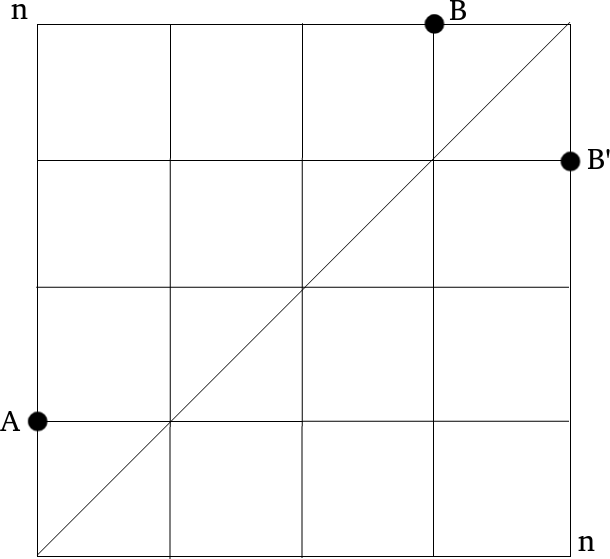
\includegraphics[width=.6\textwidth]{./pictures/4_22_1.png}
  \caption{Метод отражений}
  \label{fig:4221}
\end{figure}

Нам нужно, чтобы путь не касался диагонали,
поэтому уйдём с неё на шаг вверх в точку $A$ и будем искать количество путей из $A$ в $B$.

Количество путей из $A$ в $B$, не цепляющих диагональ,
равно общему количеству путей из $A$ в $B -$ количество путей из $A$ в $B'$.

В точку $A$ из начала координат можно попасть одним способом,
как и в конечную точку из $B$, поэтому количество путей не измениться, если начать считать с них.

Из точки $A$ в точку $B$ есть $n - 1$ вертикальный шаг и $n - 1$ горизонтальный.
Поэтому количество путей из $A$ в $B$ равно $C_{2 \left( n-1 \right)}^{n-1} = \\ = C_{2n-2}^{n-1}$.
От этого количества нужно отнять число путей,
которые пересекают диагональ (по условию задачи это те пути, у которых $S_i \leq 0$).
Когда из точки $A$ попадаем на диагональ, есть путь, симметричный данному, который ведёт в точку $B'$.
Есть $n$ горизонтальных шагов и $n - 2$ вертикальных.
Имеем $C_{n+n-2}^n = C_{2n-2}^n$ путей.

Тогда число путей из точки $ \left( 0, 0 \right) $ в точку $ \left( 2n, 0 \right) $ равно
\begin{equation*}
\begin{split}
C_{2n-2}^{n-1} - C_{2n-2}^n =
\frac{ \left( 2n-2 \right)!}{ \left( n-1 \right)! \left( 2n-2-n+1 \right)!} -
\frac{ \left( 2n-2 \right)!}{n! \left( 2n-2-n \right)!} = \\
= \frac{ \left( 2n-2 \right)!}{ \left( n-1 \right)! \left( n-1 \right)!} -
\frac{ \left( 2n-2 \right)!}{n! \left( n-2 \right)!} = \\
= \left( 2n-2 \right)!
\left( \frac{1}{ \left( n-2 \right)! \left( n-1 \right) \left( n-1 \right)! } -
\frac{1}{ \left( n-1 \right)! n \left( n-2 \right)!} \right) = \\
= \left( 2n-2 \right)! \cdot \frac{n - n + 1}{\left( n-2 \right)! \left( n-1 \right)! \left( n-1 \right) n} =
\frac{ \left( 2n-2 \right)!}{n! \left( n-1 \right)!};
\end{split}
\end{equation*}

\item данная задача аналогична предыдущей, только теперь нужно из числа путей из точки с координатами
$ \left( 0, 0 \right) $ в точку с координатами $ \left( 2n, 0 \right) $ отнять число путей, ведущих из точки $ \left( 0, 0 \right) $ в $B'$.

Из точки $ \left( 0, 0 \right) $ в точку $ \left( 2n, 0 \right) $ нужно сделать $n$ горизонтальных шагов и $n$ вертикальных --- всего $C_{2n}^{n}$.

Из точки $ \left( 0, 0 \right) $ в точку $B'$ есть $n$ горизонтальных шагов и $n - 1$ вертикальных.
Всего таких путей $C_{2n-1}^n$.

Итого имеем
\begin{equation*}
\begin{split}
C_{2n}^n - C_{2n-1}^n =
\frac{ \left( 2n \right)!}{n! n!} - \frac{ \left( 2n-1 \right)!}{n! \left( n-1 \right)!} =
\frac{ \left( 2n \right)!}{n! \left( n-1 \right)! n} - \frac{ \left( 2n-1 \right)!}{n! \left( n-1 \right)!} = \\
= \frac{ \left( 2n \right)! - \left( 2n-1 \right)! n}{n! n!} =
\frac{ \left( 2n-1 \right)! \left( 2n-n \right)}{n! n!} =
\frac{ \left( 2n-1 \right)! n}{n! n!};
\end{split}
\end{equation*}
\end{enumerate}

\item задача проиллюстрирована на рисунке \ref{fig:4222}.

\begin{figure}[h!]
  \centering
  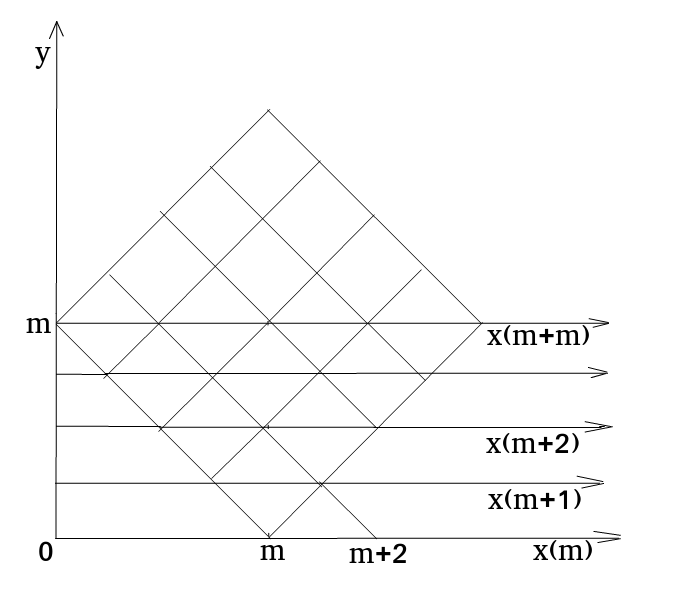
\includegraphics[width=.6\textwidth]{./pictures/4_22_2.png}
  \caption{Пути из точки $ \left( 0, m \right) $ в точку $ \left( n, 0 \right) $}
  \label{fig:4222}
\end{figure}

При $n = m$
существует один путь из точки
$ \left( 0, m \right) $
в точку
$ \left( n, 0 \right)$,
который соответствует линии,
проведённой между этими точками:
$ \left( 0, m \right) \rightarrow \\
\rightarrow \left( 1, m-1 \right) \rightarrow
\left( 2, m-2 \right) \rightarrow \dotsc \rightarrow \left( n, 0 \right)$.

При $n < m$ пути между точками с заданными условиями нет.

При $n > m$ путь возможен только при условии, что $ \left( m-n \right) mod 2 = \\ = 1$.
В каждую следующую точку, в которой выполняется это условие, существует больше путей чем в предыдущую.
Аналогично пункту а) имеем

\begin{enumerate}[label=(\roman*)]
\item
\begin{equation*}
\begin{split}
C_{m+n-2}^{n-1} - C_{m+n-2}^n =
\frac{ \left( m+n-2 \right)!}{ \left( n-1 \right)! \left( m-1 \right)!} -
\frac{ \left( m+n-2 \right)!}{n! \left( m-2 \right)!} = \\
= \frac{ \left( m+n-2 \right)!}{ \left( n-1 \right)! \left( m-2 \right)! \left( m-1 \right)} -
\frac{ \left( m+n-2 \right)!}{ \left( n-1 \right)!n \left( m-2 \right)!}= \\
= \frac{ \left( m+n-2 \right)! \left( n-m+1 \right) }{\left( n-1 \right)! \left( m-2 \right)! \left( m-1 \right) n} =
\frac{ \left( m+n-2 \right)! \left( n-m+1 \right) }{n! \left( m-1 \right)!};
\end{split}
\end{equation*}
\item 
\begin{equation*}
\begin{split}
C_{m+n}^m - C_{m+n-1}^m =
\frac{ \left( m+n \right)!}{m! n!} - \frac{ \left( m+n-1 \right)!}{m! \left( n-1 \right)!} = \\
= \frac{ \left( m+n \right)! - \left( m+n-1 \right)!n}{m!n!} =
\frac{ \left( m+n-1 \right)! \left( m+n-n \right) }{m!n!} = \\
= \frac{ \left( m+n-1 \right)! m}{m!n!}.
\end{split}
\end{equation*}
\end{enumerate}

\paragraph*{Второй способ}

Изобразим путь, который необходимо пройти в декартовых координатах (рис. \ref{fig:4223}).

\begin{figure}[h!]
  \centering
  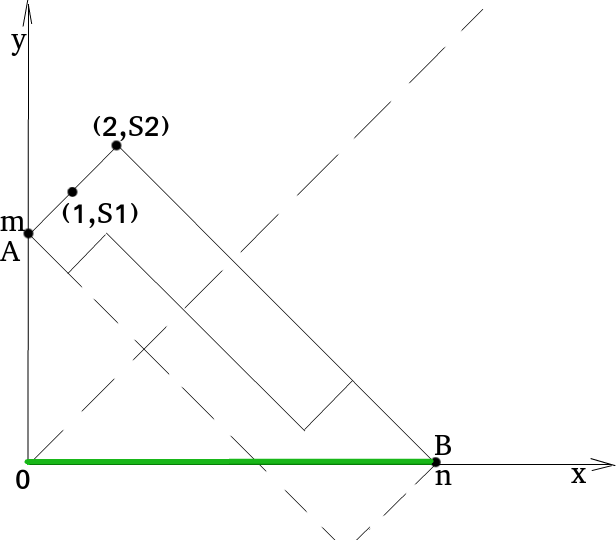
\includegraphics[width=.6\textwidth]{./pictures/4_22_3.png}
  \caption{Путь в декартовых координатах}
  \label{fig:4223}
\end{figure}

Повернём рисунок (рис. \ref{fig:4224}).

\begin{figure}[h!]
  \centering
  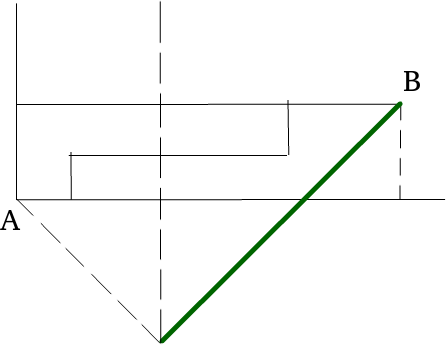
\includegraphics[width=.6\textwidth]{./pictures/4_22_4.png}
  \caption{Путь, который нужно пройти}
  \label{fig:4224}
\end{figure}

Пунктиром обозначены крайние пути, которыми можно пройтись.
Зелёным --- линия, которую нельзя пересекать.
Разница суммы шагов вниз от суммы шагов вверх будет $m$.
Для рисунка \ref{fig:4223} $AB = \sqrt{m^2 + n^2}$ --- гипотенуза треугольника $AOB$.

Самый простой случай: $m = n$ (рис. \ref{fig:4225}).

\begin{figure}[h!]
  \centering
  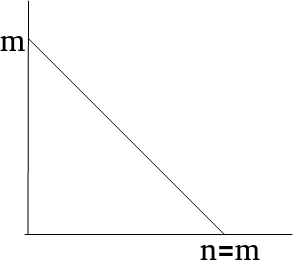
\includegraphics[width=.6\textwidth]{./pictures/4_22_5.png}
  \caption{Случай, когда $m = n$}
  \label{fig:4225}
\end{figure}

Если развернуть, получим прямоугольник шириной $m = n$ и высотой $0$.

Теперь делаем $n = m + 1$.
Высота прямоугольника $1$.
Ширина его $m + 1$.
Задача не решаема, потому что точка $n$ может быть либо под, либо над осью.
Если она под, то до неё не добраться без пересечения оси.
Если над, то она будет не на оси.

Идём дальше: $n = m + 2$.

\begin{figure}[h!]
  \centering
  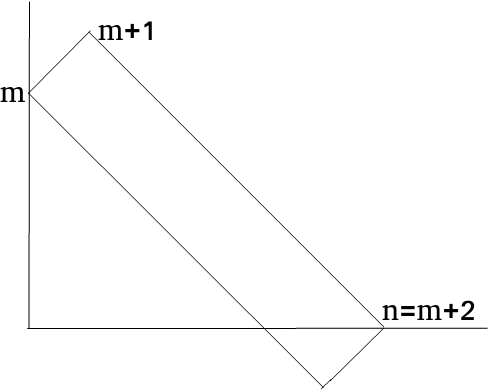
\includegraphics[width=.6\textwidth]{./pictures/4_22_6.png}
  \caption{Случай, когда $n = m + 2$}
  \label{fig:4226}
\end{figure}

Теперь $n$ на оси, форма прямоугольника не поменялась.
И т.д.
Увеличиваем $n$ на $1$ --- получаем прирост высоты и ширины на $1$, увеличиваем $n$ ещё на $1$ --- задача решаема.
Расстояние от $m$ до нижнего угла такое же, как от верхнего угла до точки $n$.
Поскольку с ростом $n$ на $2$ увеличивается $m$ на $1$, а ширина прямоугольника равна высоте этого наклонённого отрезка, то получается, что ширина результирующего прямоугольника растёт на $1$.

Проводим дополнительную вертикальную ось через $m + 2$ (рис. \ref{fig:4227}).

\begin{figure}[h!]
  \centering
  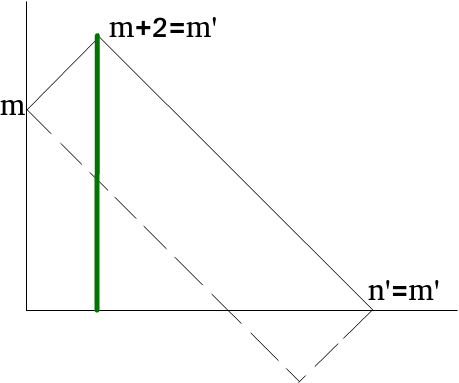
\includegraphics[width=.6\textwidth]{./pictures/4_22_7.png}
  \caption{Дополнительные построения}
  \label{fig:4227}
\end{figure}

Смотрим на верхнюю линию от $m'$ до $n'$.
Это линия длиной $m' = m + 2$.
Значит, весь предыдущий прямоугольник имеет ширину $m + 2$.
Высота 2 --- потому что двух шагов достаточно, чтобы пройтись от $m$ до $m'$.

\begin{figure}[h!]
  \centering
  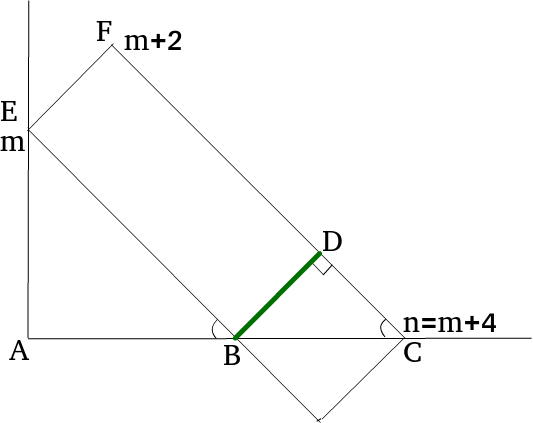
\includegraphics[width=.6\textwidth]{./pictures/4_22_8.png}
  \caption{Дополнительные построения}
  \label{fig:4228}
\end{figure}

Известно, что $AB = m, \, BC = n - m$ (рис. \ref{fig:4228}).
Угол $BCD = 45 \degree$ (можем всегда ходить направо.
При этом либо вниз, либо вверх.
Пройтись направо --- $45 \degree$).
Считаем синус:
$$ \sin \angle BCD =
\sin 45 \degree =
\frac{ \sqrt{2} }{2}.$$
Вычисляем длину $BD$ --- это катет и высота прямоугольника:
$$BD =
BC \cdot \sin \angle BCD =
\left( n-m \right) \cdot \frac{ \sqrt{2} }{2}.$$
Знаем высоту, делим её на $ \sqrt{2} $ --- получаем высоту в шагах:
$$h =
\frac{BD}{ \sqrt{2} } =
\frac{ \left( n-m \right) \sqrt{2} }{2 \sqrt{2} } =
\frac{n-m}{2}.$$

Найдём длину прямоугольника. Она состоит из отрезков $DF$ и $CD$.
$DF = BE$, поэтому найдём его длину из треугольника $ABE$:
$$BE =
\frac{AB}{ \cos \angle ABE} =
\frac{2m}{ \sqrt{2} }.$$
Найдём $CD$ из треугольника $BDC$:
$$CD =
DC \cdot \cos 45 \degree =
\left( n-m \right) \cdot \frac{ \sqrt{2} }{2}.$$
Тогда общая длина равна
\begin{equation*}
\begin{split}
CF =
BE + CD =
\frac{2m}{ \sqrt{2} } + \frac{ \left( n-m \right) \sqrt{2} }{2} =
\frac{2 \sqrt{2} m + \sqrt{2} \left( n-m \right) }{2} = \\
= \frac{ \sqrt{2} \left( 2m+n-m \right) }{2} =
\frac{ \sqrt{2} \left( n+m \right) }{2}.
\end{split}
\end{equation*}

Длина перевёрнутого прямоугольника равна
$$l =
\frac{CF}{ \sqrt{2} } =
\frac{ \sqrt{2} \left( n+m \right) }{2 \sqrt{2} } =
\frac{n+m}{2}.$$

Всего путей из $A$ в $B$ есть
\begin{equation*}
\begin{split}
C_{ \frac{n-m}{2} + \frac{n+m}{2} }^{ \frac{n-m}{2} } =
C_{ \frac{n-m+n+m}{2} }^{ \frac{n-m}{2} } =
C_n^{ \frac{n-m}{2} } =
\frac{n!}{ \left( \frac{n-m}{2} \right)! \left( n - \frac{n-m}{2} \right)! } = \\
= \frac{n!}{ \left( \frac{n-m}{2} \right)! \left( \frac{2n+m-n}{2} \right)!} =
\frac{n!}{ \left( \frac{n-m}{2} \right)! \left( \frac{n+m}{2} \right)!}. 
\end{split}
\end{equation*}

\begin{figure}[h!]
  \centering
  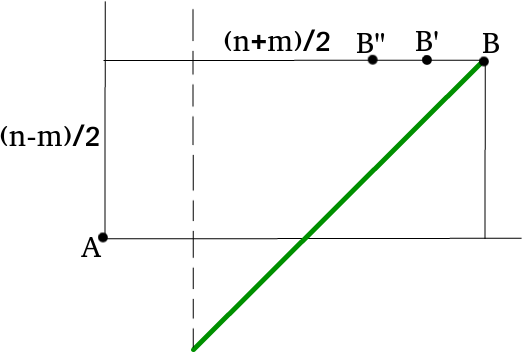
\includegraphics[width=.6\textwidth]{./pictures/4_22_9.png}
  \caption{Вспомогательный рисунок для определения количества путей}
  \label{fig:4229}
\end{figure}

\begin{enumerate}[label=(\roman*)]
\item Посчитаем количество путей, которые не касаются диагонали.
Рассмотрим частный случай.
Пусть $h = 2$ и $l = 4$.
Тогда имеем
$$C_{4+2}^2 =
C_6^2 =
\frac{6!}{2! 4!} =
\frac{5 \cdot 6}{2} =
15$$
возможных путей (рис. \ref{fig:42210}).

\begin{figure}[h!]
  \centering
  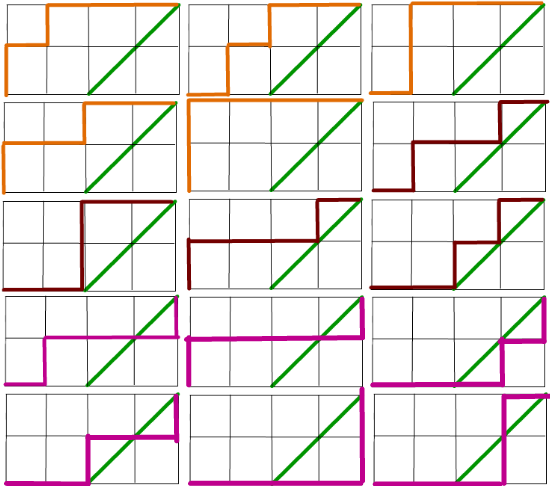
\includegraphics[width=.8\textwidth]{./pictures/4_22_10.png}
  \caption{Все возможные пути для $h = 2$ и $l = 4$}
  \label{fig:42210}
\end{figure}

Оранжевым обозначены пути, которые не касаются диагонали, коричневым --- которые только касаются диагонали, и розовым --- которые пересекают её.
Путей, которые касаются диагонали 10 --- это $C_5^2$.
Т.е. это количество путей из точки $A$ в точку $B'$.
Их
\begin{equation*}
\begin{split}
C_{ \frac{n+m}{2} + \frac{n-m}{2} - 1}^{ \frac{n-m}{2} } =
C_{ \frac{n+m+n-m-2}{2} }^{ \frac{n-m}{2} } =
C_{n-1}^{ \frac{n-m}{2} } = \\
= \frac{ \left( n-1 \right)!}{ \left( \frac{n-m}{2} \right)! \left( n - 1 - \frac{n-m}{2} \right)!} =
\frac{ \left( n-1 \right)!}{ \left( \frac{n-m}{2} \right)! \left( \frac{2n-2-n+m}{2} \right)!} =
\frac{ \left( n-1 \right)!}{ \left( \frac{n-m}{2} \right)! \left( \frac{n+m-2}{2} \right)!} = \\
= \frac{ \left( n-1 \right)!}{ \left( \frac{n-m}{2} \right)! \left( \frac{n+m}{2} - 1 \right)!}.
\end{split}
\end{equation*}

\item путей, которые пересекают диагональ --- это все пути от $A$ до $B''$, т.е.
\begin{equation*}
\begin{split}
C_{ \frac{n-m}{2} + \frac{n-m}{2} }^{ \frac{n-m}{2} } =
C_{n-m}^{ \frac{n-m}{2} } =
\frac{ \left( n-m \right)!}{ \left( \frac{n-m}{2} \right)! \left( \frac{n-m}{2} \right)! }.
\end{split}
\end{equation*}
\end{enumerate}
\end{enumerate}

\subsubsection*{4.23}

\textit{Задание.} В последний тур выборов вышли кандидаты $A$ и $B$.
Кандидат $A$ набрал $n$ голосов, кандидат $B$ --- $m$ голосов.
Избиратели голосовали последовательно.
Найдите вероятность того, что кандидат $A$ не отстал от $B$, если:
\begin{enumerate}[label=\alph*)]
\item $n \geq m$;
\item $n = m$.
\end{enumerate}
 
\textit{Решение.} Вероятность равна
$$P =
\frac{k}{| \Omega |}.$$
Общее количество путей равно $| \Omega| = C_{m+n}^m$.
Найдём $k$.

\begin{enumerate}[label=\alph*)]
\item Данная задача решена в пункте б) из предыдущей.
Так как кандидат $A$ может быть или наравне с кандидатом $B$, или лидировать, то нам подходит пункт ii).
Имеем:
\begin{equation*}
\begin{split}
C_{m+n}^m - C_{m+n-1}^m =
\frac{ \left( m+n \right)!}{m! n!} - \frac{ \left( m+n-1 \right)!}{m! \left( n-1 \right)!} = \\
= \frac{ \left( m+n \right)! - \left( m+n-1 \right)!n}{m!n!} =
\frac{ \left( m+n-1 \right)! \left( m+n-n \right) }{m!n!} = \\
= \frac{ \left( m+n-1 \right)! m}{m!n!}.
\end{split}
\end{equation*}

Тогда вероятность указанного события равна
$$P =
\frac{\frac{ \left( m+n-1 \right)! m}{m!n!}}{C_{m+n}^m} =
\frac{ \left( m+n-1 \right)! m}{m!n!} \cdot \frac{m!n!}{ \left( m+n \right)!} =
\frac{m}{m+n};$$

\item в данном случае $k = 1$.
Поэтому вероятность равна
$$P =
\frac{1}{C_{m+n}^m} =
\frac{m!n!}{ \left( m+n \right)!}.$$
\end{enumerate}

\subsubsection*{4.24}

\textit{Задание.} Решите задачу 4.12 при условии, что в начале работы в кассе буфета было $p$ монет по $50$ коп.

В буфете продаются пирожки стоимостью $50$ коп.
Около буфета собралось $m+n$ студентов,
причём $n$ из них имеют монеты по $50$ коп., а остальные $m$ имеют только по одной гривне $ \left( m \leq n \right) $.
Найдите вероятность того, что ни одному студенту не придётся ждать сдачи,
если в начале работы в кассе было $p$ монет по $50$ коп. 

\textit{Решение.} Данная задача решается методом отражений (рис. \ref{fig:423}).

\begin{figure}[h!]
  \centering
  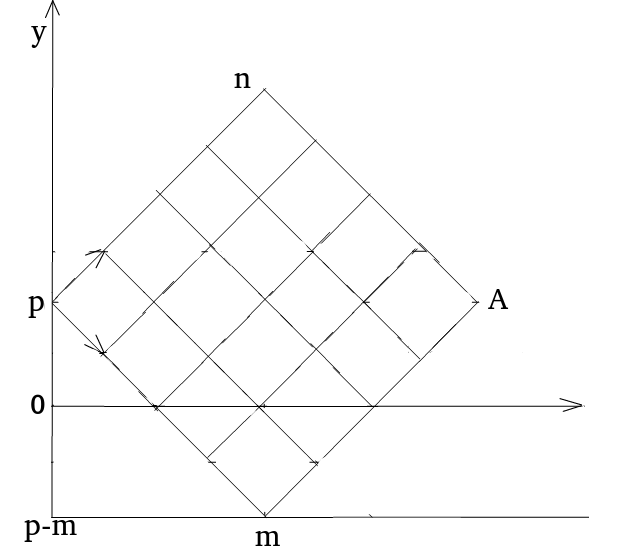
\includegraphics[width=.6\textwidth]{./pictures/4_23.png}
  \caption{Возможные исходы}
  \label{fig:423}
\end{figure}

Точка $ \left( 0, p \right) $ --- начальная, $A$ --- конечная.
Из неё можем двигаться вправо и вверх (если студент заплатил $50$ коп.) или вправо и вниз (если гривну).
Когда студент платит $50$ коп., количество монет в кассе увеличивается на единицу (становится $p + 1$).
Когда студент платит гривну, количество монет в кассе уменьшается на единицу, так как ему необходимо дать сдачу.
Их становится $p - 1$.
Всего есть $C_{n+m}^n$ путей.

Чтобы студент не ждал сдачу, монет в кассе не может быть отрицательное количество, но может быть 0.
Поэтому все пути могут касаться оси, но не пересекать её.
Таких путей 
\begin{equation*}
\begin{split}
C_{p+m}^p - C_{p+m-1}^p =
\frac{ \left( p+m \right)!}{p!m!} - \frac{ \left( p+m-1 \right)!}{p! \left( m-1 \right)!} = \\
= \frac{ \left( p+m \right)!}{p! \left( m-1 \right)! m} - \frac{ \left( p+m-1 \right)!}{p! \left( m-1 \right)!} =
\frac{ \left( p+m-1 \right)!m}{p!m!}.
\end{split}
\end{equation*}

\addcontentsline{toc}{chapter}{Занятие 5. Условные вероятности. Независимость}
\chapter*{Занятие 5. Условные вероятности. Независимость}

\addcontentsline{toc}{section}{Контрольные вопросы и задания}
\section*{Контрольные вопросы и задания}

\subsubsection*{Какие события называются независимыми?}

$A$ и $B$ --- независимы, если $P \left( A \cap B \right) = P \left( A \right) P \left( B \right) $.

\subsubsection*{Какие события называются несовместимыми?}

В теории вероятностей несколько событий называются несовместными, или несовместимыми, если никакие из них не могут появиться одновременно в результате однократного проведения эксперимента (опыта).

\subsubsection*{Запишите формулу для вычисления условной вероятности.}

Условная вероятность события $A$ при условии, что событие $B$ произошло --- это выражение
$$P \left( A/B \right) =
\frac{P \left( A \cap B \right) }{P \left( B \right) }.$$

\addcontentsline{toc}{section}{Аудиторные задачи}
\section*{Аудиторные задачи}

\subsubsection*{5.3}

\textit{Задание.} Трижды подбросили монету.
Пусть событие $A$ состоит в том, что дважды выпал герб, а событие $B$ --- в том, что хотя бы один раз выпал герб.
Найдите условные вероятности $P \left( \left. A \right| B \right), \, P \left( \left. B \right| A \right) $.
Являются ли события $A$ и $B$ независимы.

\textit{Решение.} Распишем вероятностное пространство
$$ \Omega =
\left\{ \left( 1, 1, 1 \right), \,
\left( 1, 1, 0 \right), \, \left( 1, 0, 1 \right), \, \left( 0, 1, 1 \right), \,
\left( 1, 0, 0 \right), \, \left( 0, 1, 0 \right), \, \left( 0, 0, 1 \right), \,
\left( 0, 0, 0 \right) \right\},$$
где единица означает, что выпал герб, ноль --- цифра.
На каждом из трёх мест может стоять 2 значения, поэтому $ \left| \Omega \right| = 2^3 = 8$.

Распишем событие $A = \left\{ \left( 1, 1, 0 \right), \, \left( 1, 0, 1 \right), \, \left( 0, 1, 1 \right) \right\} $.
Событие $A$ включает $ \left| A \right| = 3$ элемента.
Тогда его вероятность равна
$$P \left( A \right) =
\frac{ \left| A \right| }{ \left| \Omega \right| } =
\frac{3}{8}.$$

Распишем событие
$$B = \left\{ \left( 1, 1, 1 \right), \,
\left( 1, 1, 0 \right), \, \left( 1, 0, 1 \right), \, \left( 0, 1, 1 \right), \,
\left( 1, 0, 0 \right), \, \left( 0, 1, 0 \right), \, \left( 0, 0, 1 \right) \right\}.$$
Вероятность этого события равна
$$P \left( B \right) =
\frac{ \left| B \right| }{ \left| \Omega \right| } = 
\frac{7}{8}.$$

Найдём вероятность перечечения этих событий:
$$P \left( A \cap B \right) =
P \left\{ \left( 1, 1, 0 \right), \, \left( 1, 0, 1 \right), \, \left( 0, 1, 1 \right) \right\} =
\frac{3}{8}.$$

Найдём условную вероятность события $A$ при условии, что событие $B$ произошло:
$$P \left( \left. A \right| B \right) =
\frac{P \left( A \cap B \right) }{P \left( B \right) } =
\frac{ \frac{3}{8} }{ \frac{7}{8} } =
\frac{3 \cdot 8}{7 \cdot 8} =
\frac{3}{7}.$$

Найдём условную вероятность события $B$ при условии, что событие $A$ произошло:
$$P \left( \left. B \right| A \right) =
\frac{P \left( A \cap B \right) }{P \left( A \right) } =
\frac{ \frac{3}{8} }{ \frac{3}{8} } =
1.$$

Найдём произведение вероятностей
$$P \left( A \right) P \left( B \right) =
\frac{3}{8} \cdot \frac{7}{8} =
\frac{21}{64}.$$
Видим, что это не равно вероятности пересечения этих событий, значит события не независимы.

\subsubsection*{5.4}

\textit{Задание.} Подбрасывают два игральных кубика.
Найдите вероятность того, что выпала хотя бы одна шестёрка, если известно, что сумма очков равна 8.

\textit{Решение.}
Вероятностное пространство имеет $ \left| \Omega \right| = 6^2$ элементов, так как на каждом из двух кубиков может выпасть любая из шести цифр.
Рассмотрим событие $A =$ \{выпала хотя бы одна шестёрка\}.
Это значит, что нужно выбрать кубик, на котором выпадет шестёрка (это 2 варианта) и число, которое выпадет на оставшемся кубике --- это $6$ вариантов.
Тогда вероятность этого события равна
$$P \left( A \right) =
\frac{2 \cdot 6}{6^2} =
\frac{2}{6} =
\frac{1}{3}.$$

Рассмотрим событие $B =$ \{сумма осков равна восьми\}.
На одном кубике может выпасть двойка, тогда на втором --- восьмёрка.
Другим возможным исходом можут быть такие выпавшие цифры, как тройка и пятёрка.
Пятый вариант --- две четвёрки.
Имеем 5 вариантов.
Тогда вероятность события $B$ равна
$$P \left( B \right) =
\frac{ \left| B \right| }{ \left| \Omega \right| } =
\frac{5}{6^2} =
\frac{5}{36}.$$

Найдём вероятность пересечения этих событий:
$$P \left( A \cap B \right) =
P \left\{ \left( 2, 6 \right), \, \left( 6, 2 \right) \right\} =
\frac{2}{6^2} =
\frac{2}{36} =
\frac{1}{18}.$$

Тогда условная вероятность события $A$ при условии, что событие $B$ произошло, равна
$$P \left( \left. A \right| B \right) =
\frac{P \left( A \cap B \right) }{P \left( B \right) } =
\frac{ \frac{1}{18} }{ \frac{1}{8} } =
\frac{8}{18} =
\frac{4}{9}.$$

\subsubsection*{5.5}

\textit{Задание.}
Считая,
что рождение мальчика или девочки являются равновероятными, найдите вероятность того, что в семье с двумя детьмя оба мальчика, если известно, что
\begin{enumerate}[label=\alph*)]
\item старший ребёнок --- мальчик;
\item среди детей есть хотя бы один мальчик.
\end{enumerate}

\textit{Решение.}
Распишем пространство элементарных событий
$ \Omega = \\
= \left\{ \left( b, b \right), \, \left( b, g \right), \, \left( g, b \right), \, \left( g, g \right) \right\} $,
где $b$ означает мальчик, $g$ --- девочка, на первом месте стоит старший ребёнок, на втором --- младший.
В этом пространстве $ \left| \Omega \right| = 4$ элемента.

Пусть событие $A = \left\{ \left( b, b \right) \right\} $.

\begin{enumerate}[label=\alph*)]
\item Рассмотрим событие $B = \left\{ \left( b, g \right), \, \left(b, b \right) \right\} $.
Его вероятность равна
$$P \left( B \right) =
\frac{ \left| B \right| }{ \left| \Omega \right| } =
\frac{2}{4} =
\frac{1}{2}.$$

Рассмотрим вероятность пересечения событий $A$ и $B$.
Это будет
$$P \left( A \cap B \right) =
P \left( \left\{ \left( b, b \right) \right\} \right) =
\frac{1}{4}.$$

Тогда условная вероятность события $A$ при условии того, что событие $B$ произошло равна
$$P \left( \left. A \right| B \right) =
\frac{P \left( A \cap B \right) }{P \left( B \right) } =
\frac{ \frac{1}{4} }{ \frac{1}{2} } =
\frac{2}{4} =
\frac{1}{2};$$ 
\item рассмотрим событие $C = \left\{ \left( b, g \right), \, \left(b, b \right), \, \left( g, b \right) \right\} $.
Его вероятность равна
$$P \left( C \right) =
\frac{ \left| C \right| }{ \left| \Omega \right| } =
\frac{3}{4}.$$

Рассмотрим вероятность пересечения событий $A$ и $C$.
Это будет
$$P \left( A \cap C \right) =
P \left( \left\{ \left( b, b \right) \right\} \right) =
\frac{1}{4}.$$

Тогда условная вероятность события $A$ при условии того, что событие $C$ произошло равна
$$P \left( \left. A \right| C \right) =
\frac{P \left( A \cap C \right) }{P \left( C \right) } =
\frac{ \frac{1}{4} }{ \frac{3}{4} } =
\frac{1}{3}.$$ 
\end{enumerate}

\subsubsection*{5.6}
 
\textit{Задание.} В урне лежат $12$ красных, $8$ зелёных и $10$ синих шаров.
Из урны наугад выбирают два шара.
Найдите вероятность того, что шары разного цвета, если известно, что среди них нет синих.

\textit{Решение.} Два шара могут быть красного цвета.
Тогда есть $C_{12}^2$ способа их выбрать.
Два шара могут быть зелёного цвета --- это $C_8^2$, могут быть синего цвета --- $C_{10}^2$.
Может быть случай, когда один из шаров красный, а другой зелёный --- это $C_{12}^1 C_8^1$.
Может быть, что 1 из шаров красный, а второй синий --- это $C_{12}^1 C_{10}^1$.
Может быть случай, когда один из шаров зелёный, а второй синий --- это $C_8^1 C_{10}^1$.
По правилу произведения получаем $ \left| \Omega \right| = C_{12}^2 + C_8^2 + C_{10}^2 + C_{12}^1 C_8^1 + C_{12}^1 C_{10}^1 + C_8^1 C_{10}^1$.

Пусть событие $A =$ \{шары разного цвета\}.
Рассмотрим событие $B =$ \{среди шаров нет синих\}.
Его вероятность равна
$$P \left( B \right) =
\frac{ \left| B \right| }{ \left| \Omega \right| } =
\frac{C_{12}^2 + C_8^2 + C_{12}^1 C_8^1}{C_{12}^2 + C_8^2 + C_{10}^2 + C_{12}^1 C_8^1 + C_{12}^1 C_{10}^1 + C_8^1 C_{10}^1}.$$

Найдём вероятность пересечений событий $A$ и $B$, т.е. события $A \cap B =$ \{один из шаров красного цвета, а второй --- зелёного\}.
Она равна
$$P \left( A \cap B \right) =
\frac{ \left| A \cap B \right| }{ \left| \Omega \right| } =
\frac{C_{12}^1 C_8^1}{C_{12}^2 + C_8^2 + C_{10}^2 + C_{12}^1 C_8^1 + C_{12}^1 C_{10}^1 + C_8^1 C_{10}^1}.$$

Тогда условная вероятность события $A$ при условии, что событие $B$ произошло, равна
\begin{equation*}
\begin{split}
P \left( \left. A \right| B \right) =
\frac{P \left( A \cap B \right) }{P \left( B \right) } =
\frac{ \frac{C_{12}^1 C_8^1}{C_{12}^2 + C_8^2 + C_{10}^2 + C_{12}^1 C_8^1 + C_{12}^1 C_{10}^1 + C_8^1 C_{10}^1} }
{ \frac{C_{12}^2 + C_8^2 + C_{12}^1 C_8^1}{C_{12}^2 + C_8^2 + C_{10}^2 + C_{12}^1 C_8^1 + C_{12}^1 C_{10}^1 + C_8^1 C_{10}^1} } = \\
= \frac{C_{12}^1 C_8^1}{C_{12}^2 + C_8^2 + C_{12}^1 C_8^1}.
\end{split}
\end{equation*}

\subsubsection*{5.7}

\textit{Задание} Точка наугад выбрана в квадрате $ \left[ 0,1 \right]^2$.
Пусть
$$A =
\left\{ \xi_1 \leq \frac{1}{2} \right\}, \,
B =
\left\{ \xi_2 \leq \frac{1}{2} \right\}, \,
C =
\left\{ \left( \xi_1 - \frac{1}{2} \right) \left( \xi_2 - \frac{1}{2} \right) < 0 \right\}.$$
Выясните, являются ли эти события независимыми:
\begin{enumerate}[label=\alph*)]
\item попарно;
\item в совокупности.
\end{enumerate}

\textit{Решение} Опишем вероятностное пространство $ \Omega = \left[ 0,1 \right]^2$.
Его площадь равна $S_{ \Omega } = 1 \cdot 1 = 1$.
Событию
$$A =
\left\{ \xi_1 \leq \frac{1}{2} \right\} $$
способствуют все точки квадрата, расположенные не правее вертикальной прямой
$$ \xi_1 \leq \frac{1}{2}.$$
Событие $A$ --- это прямоугольник со сторонами длиной $1$ и $1/2$.
Его площадь равна
$$S_A =
1 \cdot \frac{1}{2} =
\frac{1}{2}.$$
Тогда вероятность события $A$ равна
$$P \left( A \right) =
\frac{S_A}{S_{ \Omega }} =
\frac{ \frac{1}{2} }{1} =
\frac{1}{2}.$$

Событию $B$ способствуют точки квадрата, расположенные ниже горизонтальной прямой
$$ \xi_2 = \frac{1}{2}.$$
Это прямоугольник о сторонами длиной $1$ и $1/2$.
Его площадь равна
$$S_B =
1 \cdot \frac{1}{2} =
\frac{1}{2}.$$
Тогда вероятность события $B$ равна
$$P \left( B \right) =
\frac{S_B}{S_{ \Omega }} =
\frac{ \frac{1}{2} }{1} =
\frac{1}{2}.$$

Событию $C$ способствуют 2 квадрата со сторонами длиной $1/2$.
Их площадь равна
$$S_C =
2 \cdot \frac{1}{2} \cdot \frac{1}{2} =
\frac{1}{2}.$$
Тогда вероятность события $C$ равна
$$P \left( C \right) =
\frac{S_C}{S_{ \Omega }} =
\frac{ \frac{1}{2} }{1} =
\frac{1}{2}.$$

\begin{enumerate}[label=\alph*)]
\item Найдём вероятность пересечения события $A$ и $B$.
Это будет
$$P \left( A \cap B \right) =
P \left( \left\{ \xi_1 \leq \frac{1}{2}, \, \xi_2 \leq \frac{1}{2} \right\} \right) =
\frac{1}{4},$$
т.к. эти точки образуют квадрат со сторонами $1/2$.
Видим, что
$$P \left( A \cap B \right) =
P \left( A \right) P \left( B \right) =
\frac{1}{4},$$
поэтому события независимы.

Найдём вероятность пересечения события $A$ и $С$.
Это будет
$$P \left( A \cap C \right) =
P \left( \left\{ \xi_1 \leq \frac{1}{2}, \, \left( \xi_1 - \frac{1}{2} \right) \left( \xi_2 - \frac{1}{2} \right) < 0 \right\} \right) =
\frac{1}{4},$$
т.к. эти точки образуют квадрат со сторонами $1/2$.
Видим, что
$$P \left( A \cap C \right) =
P \left( A \right) P \left( C \right) =
\frac{1}{4},$$
поэтому события независимы.

Найдём вероятность пересечения события $C$ и $B$.
Это будет
$$P \left( C \cap B \right) =
P \left( \left\{ \left( \xi_1 - \frac{1}{2} \right) \left( \xi_2 - \frac{1}{2} \right) < 0, \, \xi_2 \leq \frac{1}{2} \right\} \right) =
\frac{1}{4},$$
т.к. эти точки образуют квадрат со сторонами $1/2$.
Видим, что
$$P \left( C \cap B \right) =
P \left( C \right) P \left( B \right) =
\frac{1}{4},$$
поэтому события независимы;
\item найдём вероятность пересечения всех трёх событий:
\begin{equation*}
\begin{split}
P \left( A \cap B \cap C \right) = \\
= P \left( \left\{ \xi_1 \leq \frac{1}{2}, \,
\xi_2 \leq \frac{1}{2}, \,
\left( \xi_1 - \frac{1}{2} \right) \left( \xi_2 - \frac{1}{2} \right) < 0\right\} \right) =
0.
\end{split}
\end{equation*}
События не являются независимыми в совокупности, так как
$$P \left( A \cap B \cap C \right) =
0 \neq
P \left( A \right) P \left( B \right) P \left( C \right) =
\frac{1}{8}.$$
\end{enumerate}

\subsubsection*{5.8}

\textit{Задание.} Докажите, что
$P \left( A_1 \dotsc A_n \right) = \\
= P \left( A_1 \right) P \left( \left. A_2 \right| A_1 \right) \dotsc P \left( \left. A_n \right| A_1 A_2 \dotsc A_{n-1} \right) $.

\textit{Решение.} Распишем правую часть по формуле условной вероятности:
\begin{equation*}
\begin{split}
P \left( A_1 \right) P \left( \left. A_2 \right| A_1 \right) \dotsc P \left( \left. A_n \right| A_1 A_2 \dotsc A_{n-1} \right) =
P \left( A_1 \right) \cdot
\frac{P \left( A_1 \cap A_2 \right) }{P \left( A_1 \right) } \cdot
\dotsc \times \\
\times \frac{P \left( A_1 A_2 \dotsc A_{n-1} A_n \right) }{P \left( A_1 A_2 \dotsc A_{n-1} \right) } =
P \left( A_1 A_2 \dotsc A_{n-1} A_n \right).
\end{split}
\end{equation*}

\subsubsection*{5.9}

\textit{Задание.}
Пусть $P \left( A \right) \in \left( 0,1 \right) $ и $P \left( \left. B \right| \overline{A} \right) = P \left( \left. B \right| A \right) $.
Докажите, что $A$ и $B$ независимы.

\textit{Решение.} Распишем условные вероятности:
$$P \left( \left. B \right| \overline{A} \right) =
\frac{P \left( B \cap \overline{A} \right) }{P \left( \overline{A} \right) } =
\frac{P \left( B \cap A \right)}{P \left( A \right) } =
P \left( \left. B \right| A \right).$$

Известно, что $P \left( \overline{A} \right) = 1 - P \left( A \right) $, поэтому
$$\frac{P \left( B \cap \overline{A} \right) }{1 - P \left( A \right) } =
\frac{P \left( B \cap A \right)}{P \left( A \right) }.$$

По формуле разницы множеств: $P \left( B \setminus A \right) = P \left( B \cap \overline{A} \right) $ получаем:
$$\frac{P \left( B \setminus A \right) }{1 - P \left( A \right) } =
\frac{P \left( B \cap A \right)}{P \left( A \right) }.$$

Так как $P \left( B \setminus A \right) = P \left( B \right) - P \left( A \cap B \right) $, то
$$\frac{P \left( B \right) - P \left( A \cap B \right) }{1 - P \left( A \right) } =
\frac{P \left( B \cap A \right)}{P \left( A \right) }.$$

Перемножим как пропорцию:
$P \left( A \right) \left( P \left( B \right) - P \left( A \cap B \right) \right) = \\
= P \left( A \cap B \right) \left( 1 - P \left( A \right) \right) $.

Раскроем скобки:
$P \left( A \right) P \left( B \right) - P \left( A \right) P \left( A \cap B \right) =
P \left( A \cap B \right) - \\ - P \left( A \cap B \right) P \left( A \right) $.

Уничтожим одинаковые члены: $P \left( A \right) P \left( B \right) = P \left( A \cap B \right) $.
Это значит, что события $A$ и $B$ независимы.

\subsubsection*{5.10}

\textit{Задание.} Докажите, что если событие $A$ не зависит само от себя, то или $P \left( A \right) = 1$, или $P \left( A \right) = 0$.

\textit{Решение.}
События независимы, когда вероятность пересечения равна пересечению вероятностей:
$P \left( A \cap A \right) =
P \left( A \right) P \left( A \right) =
\left( P \left( A \right) \right)^2 =
P \left( A \right) $.

Квадрат числа равен числу, когда оно равно или нулю, или единице.

\subsubsection*{5.11}

\textit{Задание.} Вероятность того, что компьютер №1 проработает месяц без поломок равна $0.9$, для компьютера №2 эта вероятность равна $0.8$.
Компьютеры работают независимо друг от друга.
Найдите вероятность того, что за месяц работы:
\begin{enumerate}[label=\alph*)]
\item оба компьютера не поломаются;
\item оба компьютера поломаются;
\item поломается хотя бы один компьютер;
\item поломается только компьютер №2;
\item поломается один и только один из компьютеров.
\end{enumerate}

\textit{Решение.} Пусть событие $A =$ \{компьютер №1 не поломается\}, а событие $B =$ \{компьютер №2 не поломается\}.
Их вероятности по условию равны $P \left( A \right) = 0.9$ и $P \left( B \right) = 0.8$.
\begin{enumerate}[label=\alph*)]
\item Вероятность того, что оба компьютера не поломаются равна
$P \left( A \cap B \right) = \\
= P \left( A \right) P \left( B \right) =
0.9 \cdot 0.8 =
0.72$;
\item событие \{оба компьютера поломаются\} означает, что не произойдёт ни событие $A$, ни событие $B$.
Вероятность такого события равна
\begin{equation*}
\begin{split}
P \left( \overline{A} \cap \overline{B} \right) =
P \left( \overline{A} \right) P \left( \overline{B} \right) =
\left( 1 - 0.9 \right) \left( 1 - 0.8 \right) =
0.1 \cdot 0.2 =
0.02;
\end{split}
\end{equation*} 
\item данное событие означает, что произойдёт хотя бы одно из событий $\overline{A}$ или $ \overline{B}$.
По формуле включений-исключений имеем:
$P \left( \overline{A} \cup \overline{B} \right) = \\
= P \left( \overline{A} \right) + P \left( \overline{B} \right) - P \left( \overline{A} \cap \overline{B} \right) =
1 - 0.9 + 1 - 0.8 - 0.02 =
0.1 + 0.2 - 0.02 = \\
= 0.3 - 0.02 =
0.298$;
\item событие означает, что произошло событие $A$ и не произошло событие $B$.
Вероятность этого равна
$P \left( A \cap \overline{B} \right) =
P \left( A \right) P \left( \overline{B} \right) =
0.9 \cdot \left( 1 - 0.8 \right) = \\
= 0.9 \cdot 0.2 =
0.18$;
\item событие означает, что произойдёт или событие $A$, или событие $B$.
Вероятность того, что поломается только компьютер №1 равна
$$P \left( \overline{A} \cap B \right) =
P \left( \overline{A} \right) P \left( B \right) =
\left( 1 - 0.9 \right) \cdot 0.2 =
0.1 \cdot 0.2 =
0.02.$$
Вероятность того, что поломается только компьютер №2 равна
$$P \left( A \cap \overline{B} \right) =
P \left( A \right) P \left( \overline{B} \right) =
0.9 \cdot \left( 1 - 0.8 \right) =
0.9 \cdot 0.2 =
0.18.$$
Нужно найти сумму этих вероятностей: $0.02 + 0.18 = 0.2$.
\end{enumerate}

\subsubsection*{5.12}

\textit{Задание.} Вероятность того, что хотя бы один из четырёх сигналов будет передан правильно, равна $0.9984$.
Найдите вероятность правильной передачи одного сигнала, если сигналы передаются независимо друг от друга.

\textit{Решение.} Вероятность того, что ни один из сигналов не будет передан правильно, равна $1 - 0.9984 = 0.0016$.
Эта вероятность равна сумме четырёх вероятностей того, что сигнал не будет передан правильно, т.е. вероятность того,
что один сигнал не будет передан правильно, равна $0.0016/4 = 0.04$.
Тогда вероятность того, что 1 сигнал будет передан правильно, равна $1 - \\ - 0.04 = 0.96$.

\subsubsection*{5.13}

\textit{Задание.} Для некоторой группы людей из 60 человек данные о том, сколько человек курят и не курят и сколько из них имеют и не имеют рак лёгких отображены в таблице:
\begin{center}
\begin{tabular}{|l|l|l|l|}
\hline
& Не курит & Курит & Всего \\ \hline
Не болеет раком & 40 & 10 & 50 \\ \hline
Болеет раком & 7 & 3 & 10 \\ \hline
Всего & 47 & 13 & 60 \\
\hline
\end{tabular}
\end{center}
Проанализовав данные в таблице,
выясните, являются ли события $X = \\ =$ \{человек болеет раком\} и П = \{человек курит\} независимыми для данной группы людей.

\textit{Решение} Из таблицы видим, что $ \left| X \right| = 10$, при этом $\left| \Omega \right| = 60$.
Поэтому
$$P \left( X \right) =
\frac{ \left| X \right| }{ \left| \Omega \right| } =
\frac{10}{60} =
\frac{1}{6}.$$

Аналогично $ \left| \prod \right| = 13$.
Поэтому вероятность равна
$$P \left( \Pi \right) =
\frac{ \left| \Pi \right| }{ \left| \Omega \right| } =
\frac{13}{60}.$$

Найдём произведение этих вероятностей:
$$P \left( X \right) P \left( \Pi \right) =
\frac{1}{6} \cdot \frac{13}{60} =
\frac{13}{360} =
\frac{1}{27}.$$

Найдём вероятность пересечения этих двух событий.
Пересечение содержит $ \left| X \cap \Pi \right| = 3$.
Тогда вероятность равна
$$P \left( X \cap \Pi \right) =
\frac{3}{60} =
\frac{1}{20}.$$

События не являются независимыми, так как
$$ \frac{1}{27} \neq \frac{1}{20}.$$

\addcontentsline{toc}{section}{Дополнительные задачи}
\section*{Дополнительные задачи}

\subsubsection*{5.14}

\textit{Задание.}
Докажите, что события
$A_1, \dotsc, A_n$,
которые заданы на одном вероятностном пространстве,
независимы тогда и только тогда,
когда выполняется $2^n$ условий:
$P \left( A_1^{ \delta_1} \dotsc A_n^{ \delta_n} \right) =
P \left( A_1^{ \delta_1} \right) \dotsc P \left( A_n^{ \delta_n} \right) $, где
$$ \delta_i \in \left\{ 0, 1 \right\}; \, A_i^{ \delta_i} =
\begin{cases}
A_i, \, \delta_i = 1, \\
\overline{A_i}, \, \delta_i = 0,
\end{cases}
i = \overline{1, n}.$$

\textit{Решение.} Рассмотрим $n$ случайных событий таких, что любые $n-1$ их них независимы, а все $n$ --- зависимы.

Рассмотрим полный граф с $n$ вершинами ($n$ точек на плоскости, между которыми проведены все возможные рёбра).
На каждом ребре случайным образом выбрано направление.
Получился ориентированный граф (рис. \ref{fig:514}).

\begin{figure}[h!]
  \centering
  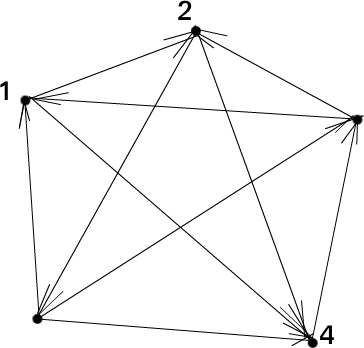
\includegraphics[width=.4\textwidth]{./pictures/5_14.png}
  \caption{Ориентированный граф}
  \label{fig:514}
\end{figure}

Пускай $r_i$ --- количество стрелок, ведущих в $i$-ую вершину.
Например, $r_1 = 2, \, r_4 = 3$.
Событие $A_i =$ \{$r_i$ --- чётное\}.
Утверждаем, что имеют место свойства:
\begin{itemize}
\item $A_1, \dotsc, A_n$ --- зависимые:
$$r_1 + r_2 + \dotsc + r_n =
\frac{n \left( n+1 \right) }{2}$$
(общее количество стрелок, которое равно количеству рёбер);
\item любые $n - 1$ события независимы.
\end{itemize}

Рассмотрим $A_1, \dotsc, A_n$.
Найдём вероятность $A_1$.
Начнём с описания вероятностного пространства.
Имеем дело с классическим экспериментом.
$ \Omega =$ \{все возможные ориентации графа\}, $ \left| \Omega \right| = 2^{ \frac{n \left( n-1 \right) }{2} }$.
Докажем, что $ \left| A_1 \right| = \left| \overline{A_1} \right| $.
Если сумеем построить биекицию (рис. \ref{fig:5141}), то $ \left| A_1 \right| = \left| \overline{A_1} \right| $.

\begin{figure}[h!]
  \centering
  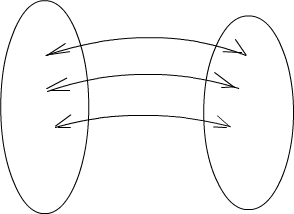
\includegraphics[width=.4\textwidth]{./pictures/5_14_1.png}
  \caption{Слева --- ориентации, в которых $r_1$ --- чётное, справа --- ориентации, в которых $r_1$ --- нечётное}
  \label{fig:5141}
\end{figure}

Все стрелки оставляем, а стрелку на ребре $1, 2$ меняем на противоположную (рис. \ref{fig:5142}).

\begin{figure}[h!]
  \centering
  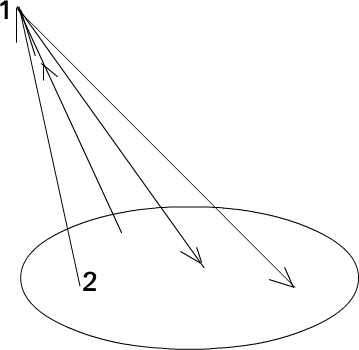
\includegraphics[width=.4\textwidth]{./pictures/5_14_2.png}
  \caption{Построение биекции}
  \label{fig:5142}
\end{figure}

Таким образом получим плохую ориентацию, при которой в вершину 1 будет идти нечётное количество стрелок --- взаимно однозначное отражение.
$$P \left( A_1 \right) =
\frac{1}{2}, \, P \left( A_1^{ \epsilon_1 } \cap A_2^{ \epsilon_2} \cap \dotsc \cap A_{n-1}^{ \epsilon_{n-1} } \right) =
\frac{1}{2^{n-1}}.$$
Проверим для $P \left( A_1 \cap A_2 \cap \dotsc \cap A_{n-1} \right) $ (рис. \ref{fig:5143}).

\begin{figure}[h!]
  \centering
  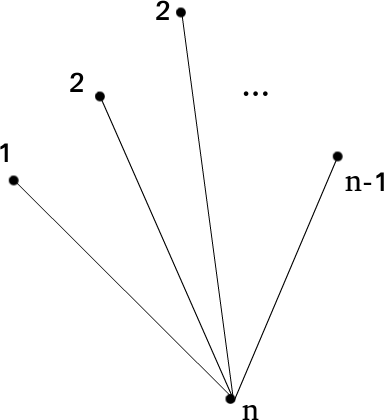
\includegraphics[width=.4\textwidth]{./pictures/5_14_3.png}
  \caption{Построение биекции}
  \label{fig:5143}
\end{figure}

Покажем, что
$ \left| A_1^{ \epsilon_1 } \cap \dotsc \cap A_{n-1}^{ \epsilon_{n-1} } \right| =
\left| A_1 \cap \dotsc \cap A_{n-1} \right| \,
\forall \epsilon_1, \dotsc, \epsilon_{n-1} =
\pm 1$.
Фиксируем все возможные наборы чётности.
При разных наборах $A_i$ и $ \overline{A_i} $ не пересекаются.
Должны научиться устанавливать биекцию.
Есть ориентация, из которой хотим получить хорошую.
Взаимно-однозначное соответствие устанавливается путём перевыбора направлений рёбер, ведущих из $n$-ой вершины во все остальные.
$ \bigcup \limits_{ \epsilon_1, \dotsc, \epsilon_{n-1} \pm 1} A_1^{ \epsilon_1 \cap \dotsc \cap A_{n-1}^{ \epsilon_{n-1} }} =
\Omega, \\
P \left( A_1 \cap \dotsc \cap A_{n-1} \right) =
\frac{1}{2^{n-1}}.$

\addcontentsline{toc}{section}{Домашнее задание}
\section*{Домашнее задание}

\subsubsection*{5.15}

\textit{Задание.} Из колоды игральных карт наугад вынута одна карта.
Найдите вероятность того, что:
\begin{enumerate}[label=\alph*)]
\item эта карта является красной масти, при условии, что она является красной;
\item порядок карты является выше чем 10, если известно, что она красной масти;
\item эта карта является тузом, если известно, что она является красной.
\end{enumerate}

\textit{Решение.} 
\begin{enumerate}[label=\alph*)]
\item Нужно найти вероятность события $A$ при условии выполнения события $B$.
Опишем оба события.
Событие $A =$ \{вынута карта красной масти\}.
Красных карт половина от всего количества.
Событие $B =$ \{карта является красной\}.
Видим, что события $A$ и $B$ идентичны, поэтому $P \left( A \cap B \right) = P \left( A \right) = P \left( B \right)$.
Тогда условная вероятность события равна
$$P \left( A/B \right) =
\frac{P \left( A \cap B \right)}{P \left( B \right) } =
\frac{ \frac{1}{2} }{ \frac{1}{2} } =
1;$$
\item нужно найти вероятность события $A$ при условии выполнения события $B$.
Опишем оба события.
Событие $A =$ \{порядок выбранной карты больше десяти\}.
Такими картами является валет, дама, король и туз любой масти.
Событие $B =$ \{карта является красной\}.
Его вероятность равна
$$P \left( B \right) =
\frac{1}{2}.$$
Пересечение событий $A$ и $B$ даёт такие карты как валет, дама, король и туз красных мастей.
Вероятность пересечения равна
$$P \left( A \cap B \right) =
\frac{2 \cdot 4}{52} =
\frac{4}{26} =
\frac{2}{13}.$$
Тогда условная вероятность события равна
$$P \left( A/B \right) =
\frac{P \left( A \cap B \right)}{P \left( B \right) } =
\frac{ \frac{2}{13} }{ \frac{1}{2} } =
\frac{4}{13};$$
\item нужно найти вероятность события $A$ при условии выполнения события $B$.
Опишем оба события.
Событие $A =$ \{карта является тузом\}.
Такими картами являются 4 туза.
Событие $B =$ \{карта является красной\}.
Его вероятность равна
$$P \left( B \right) =
\frac{1}{2}.$$
Пересечение событий $A$ и $B$ даёт два красных туза.
Вероятность пересечения равна
$$P \left( A \cap B \right) =
\frac{2}{52} =
\frac{1}{26}.$$
Тогда условная вероятность события равна
$$P \left( A/B \right) =
\frac{P \left( A \cap B \right)}{P \left( B \right) } =
\frac{ \frac{1}{26} }{ \frac{1}{2} } =
\frac{2}{26} =
\frac{1}{13}.$$
\end{enumerate}

\subsubsection*{5.16}

\textit{Задание.} Игральный кубик подбросили дважды.
Найдите вероятность того, что сумма очков является больше 7, если известно, что:

\begin{enumerate}[label=\alph*)]
\item при первом подбрасывании быпало одно очко;
\item при первом подбрасывании выпало меньше, чем 5 очков.
\end{enumerate}

\textit{Решение.}
Вероятностное пространство эксперимента,
который состоит в подбрасывании игрального кубика дважды,
опишем множеством
$ \Omega = \\
= \left\{ \left( x, y \right), \, x = \overline{1, 6}, \, y = \overline{1, 6} \right\} $,
где через $x$ обозначим количество очков,
которые выпали при первом подбрасывании игрального кубика, а через $y$ --- количество очков, которые выпали при втором его подбрасывании.
Нам нужно вычислить вероятности $P \left( \left. x+y>7 \right| x=1 \right) $ и $P \left( \left. x+y>7 \right| x<5 \right) $.
По определению вероятности:
$$P \left( \left. x+y>7 \right| x=1 \right) =
\frac{P \left( x+y>7, \, x=1 \right) }{P \left( x=1 \right) }.$$
Поскольку
$ \left\{ \left( x, y \right) \in \Omega: \, x + y > 7, \, x = 1 \right\} =
\varnothing $,
а $ \left\{ \left( x, y \right) \in \Omega: \, x = 1 \right\} =  \\ = \left\{ \left( 1, y \right), \, y = \overline{1, 6} \right\} $, то
$$P \left( \left. x+y>7 \right| x=1 \right) =
\frac{0}{ \frac{6}{36} } =
0.$$
Далее
$$P \left( \left. x+y>7 \right| x<5 \right) =
\frac{P \left( x+y>7, x<5 \right) }{P \left( x<5 \right) }.$$
Понятно, что
$$P \left( x<5 \right) =
\frac{4}{6} =
\frac{2}{3}.$$
А для вероятности в числителе имеем:
\begin{equation*}
\begin{split}
P \left( x+y>7, x<5 \right) =
\sum \limits_{k=1}^4 P \left(x=k, \, k+y>7 \right) = \\
= \sum \limits_{k=1}^4 P \left( x=k \right) P \left( y>7-k \right) =
P \left( x=1 \right) P \left( y>6 \right) +
P \left( x=2 \right) P \left( y>5 \right) + \\
+ P \left( x=3 \right) P \left( y>4 \right) +
P \left( x=4 \right) P \left( y>3 \right) =
\frac{1}{6} \left( 0 +\frac{1}{6} + \frac{2}{6} + \frac{3}{6} \right) =
\frac{1}{6} \cdot \frac{6}{6} = \\
= \frac{6}{36} =
\frac{1}{6}.
\end{split}
\end{equation*}

Тут мы воспользовались тем, что результаты первого и второго подбрасываний являются независимыми событиями.
Таким образом:
$$P \left( \left. x+y>7 \right| x<5 \right) =
\frac{P \left( x+y>5, \, x<5 \right) }{P \left( x<5 \right) } =
\frac{ \frac{1}{6} }{ \frac{2}{3} } =
\frac{1}{4}.$$

\subsubsection*{5.17}

\textit{Задание.} Дважды подброшена монета.
Рассмотрим следующие события:
$A =$ \{при первом подбрасывании выпала решка\}, $B =$ \{при втором подбрасывании выпала решка\}, $C =$ \{результат обоих подбрасываний одинаковый\}.
Покажите, что события $A, \, B, \, C$ попарно независимы, но не независыми в совокупности.

\textit{Решение.} События $A_i$ и $A_j$ называются попарно независимыми, если для $ \forall i \neq j \rightarrow A_i $ и $A_j$ --- независимы.

Пространством элементарных исходов является множество векторов
$ \Omega = \\
= \left\{ \left( i, j \right), \, i, j \in \left\{ 0, 1 \right\} \right\}$,
где $0$ означает, что выпал герб, $1$ --- выпала решка, $i$ --- результат первого подбрасывания, $j$ --- результат второго подбрасывания.
Пространство элементарных событий содержит $ \left| \Omega \right| = 2^2 = 4$ элемента.

Опишем данные события.
Событие $A = \left\{ \left( 1, 0 \right), \, \left( 1, 1 \right) \right\} $.
Вероятность выпадения при первом подбрасывании решки равна
$$P \left( A \right) =
\frac{2}{4} =
\frac{1}{2}.$$

Опишем событие $B = \left\{ \left( 0, 1 \right), \, \left( 1, 1 \right) \right\} $.
Вероятность выпадения решки при втором подбрасывании равна
$$P \left( B \right) =
\frac{2}{4} =
\frac{1}{2}.$$

Опишем событие $C = \left\{ \left( 0, 0 \right), \, \left( 1, 1 \right) \right\} $.
Вероятность того, что результат двух подбрасываний будет одинаковым, равна
$$P \left( C \right) =
\frac{2}{4} =
\frac{1}{2}.$$

Найдём вероятность пересечения событий $A$ и $B$:
$$P \left( A \cap B \right) =
P \left( \left\{ \left( 1, 1 \right) \right\} \right) =
\frac{1}{4}.$$
Найдём произведение вероятностей этих событий:
$$P \left( A \right) P \left( B \right) =
\frac{1}{2} \cdot \frac{1}{2} =
\frac{1}{4}.$$
Получаем, что $P \left( A \cap B \right) = P \left( A \right) P \left( B \right) $, значит эти события независимы.

Найдём вероятность пересечения событий $A$ и $C$:
$$P \left( A \cap C \right) =
P \left( \left\{ \left( 1, 1 \right) \right\} \right) =
\frac{1}{4}.$$
Найдём произведение вероятностей этих событий:
$$P \left( A \right) P \left( C \right) =
\frac{1}{2} \cdot \frac{1}{2} =
\frac{1}{4}.$$
Получаем, что $P \left( A \cap C \right) = P \left( A \right) P \left( C \right) $, значит эти события независимы.

Найдём вероятности пересечения событий $B$ и $C$:
$$P \left( B \cap C \right) =
P \left( \left\{ \left( 1, 1 \right) \right\} \right) =
\frac{1}{4}.$$
Найдём произведение вероятностей этих событий:
$$P \left( B \right) P \left( C \right) =
\frac{1}{2} \cdot \frac{1}{2} =
\frac{1}{4}.$$
Получаем, что $P \left( B \cap C \right) = P \left( B \right) P \left( C \right) $, значит эти события независимы.

События $A, \, B, \, C$ называются независимыми в совокупности, если имеет место равенство:
$P \left( A \cap B \cap C \right) =
P \left( A \right) P \left( B \right) P \left( C \right) $.

Проверим это равенство для данной задачи:
$$P \left( A \cap B \cap C \right) =
P \left( \left\{ \left( 1, 1 \right) \right\} \right) =
\frac{1}{4}.$$
Найдём произведение вероятностей всех трёх событий:
$$P \left( A \right) P \left( B \right) P \left( C \right) =
\frac{1}{2} \cdot \frac{1}{2} \cdot \frac{1} {2} =
\frac{1}{8}.$$
Получили, что равенство не выполняется, поэтому события не независимы.

\subsubsection*{5.18}

\textit{Задание.} В урне $7$ белых и $3$ чёрных шарика.
Из неё наугад вынимают три шарика.
Известно, что среди них есть чёрный шарик.
Найдите вероятность того, что два других шарика белые.

\textit{Решение.}
Пространство элементарных событий имеет вид
$ \Omega = \\ = \left\{ \left( i, j, k \right): i, j, k \in \right.$ \{белый, чёрный\}, где $i, j, k$ --- цвета вытянутых шариков\}.
Выпишем все его элементы: $ \Omega = $ \{(чёрный, чёрный, чёрный), (чёрный, белый, белый), (белый, чёрный, белый), (белый, белый, чёрный),
(чёрный, чёрный, белый), (чёрный, белый, чёрный), (белый, чёрный, чёрный), (белый, белый, белый)\}.
Видим, что $ \left| \Omega \right| = 2^3 = 8$.

Событие $B =$ \{среди выбранных шаров есть чёрный шар\} = \{(чёрный, чёрный, чёрный),
(чёрный, белый, белый), (белый, чёрный, белый), (белый, белый, чёрный),
(чёрный, чёрный, белый), (чёрный, белый, чёрный), (белый, чёрный, чёрный)\}.
Вероятность этого события равна
$$P \left( B \right) =
\frac{ \left| B \right| }{ \left| \Omega \right| } =
\frac{7}{8}.$$

Опишем событие $A =$ \{два шара белые\} = \{(чёрный, белый, белый), (белый, чёрный, белый), (белый, белый, чёрный), (белый, белый, белый)\}.

Найдём вероятность пересечения событий $A$ и $B: \, P \left( A \cap B \right) =$ \{(чёрный, белый, белый), (белый, чёрный, белый), (белый, белый, чёрный)\}.

Тогда условная вероятность события $A$ при условии, что $B$ произошло равна
$$P \left( A/B \right) =
\frac{P \left( A \cap B \right) }{P \left( B \right) } =
\frac{ \frac{3}{8} }{ \frac{7}{8} } =
\frac{3}{7}.$$

\subsubsection*{5.19}

\textit{Задание.} Точка $ \xi = \left( \xi_1, \xi_2 \right) $ наугад выбрана в квадрате $ \left[ 0, 1 \right]^2$.
Пусть $B = \\ = \left\{ \xi_1 + \xi_2 \leq 1 \right\} $.
Вычислите условную вероятность $P \left( \left. A \right| B \right) $, если:
\begin{enumerate}[label=\alph*)]
\item $A = \left\{ \left| \xi_1 + \xi_2 \right| < 1 \right\} $;
\item $A = \left\{ \xi_1 \cdot \xi_2 < 1/2 \right\} $;
\item $A = \left\{ \max \left\{ \xi_1, \xi_2 \right\} < 1/2 \right\} $;
\item $A = \left\{ \xi_1^2 + \xi_2^2 < 1/4 \right\} $;
\item $A = \left\{ \xi_1 > \xi_2 \right\} $.
\end{enumerate}

\textit{Решение.}
Вероятностное пространство эксперимента,
который состоит в выборе точки в квадрате
$ \left[ 0, 1 \right]^2$, опишем множеством
$$ \Omega =
\left\{ \left( \xi_1, \xi_2 \right), \,
0 \leq \xi_1 \leq 1, \,
0 \leq \xi_2 \leq 1 \right\},$$
где через $ \xi_1$ обозначена первая координата точки, а через $ \xi_2$ --- вторая координата.

Вычислим вероятность события $B$.
Это прямоугольный равнобедренный треугольник с катетами длиной $1$.
Тогда площадь этой фигуры равна
$$S_B =
\frac{1}{2} \cdot 1 \cdot 1 =
\frac{1}{2}.$$

\begin{enumerate}[label=\alph*)]
\item Событие $A$ --- это прямоугольный равнобедренный треугольник с катетами длиной $1$.
Вероятность пересечения событий $A$ и $B$ равна
$$P \left( A \cap B \right) =
\frac{1}{2}.$$
Тогда условная вероятность равна
$$P \left( \left. A \right| B \right) =
\frac{P \left( A \cap B \right) }{P \left( B \right) } =
\frac{ \frac{1}{2} }{ \frac{1}{2} } =
1;$$
\item событие $A$ --- это часть квадрата под веткой гиперболы
$$ \xi_2 = \frac{1}{2 \xi_1}.$$
Вероятность пересечения событий $A$ и $B$ равна
$$P \left( A \cap B \right) =
\frac{1}{2}.$$
Тогда условная вероятность равна
$$P \left( \left. A \right| B \right) =
\frac{P \left( A \cap B \right) }{P \left( B \right) } =
\frac{ \frac{1}{2} }{ \frac{1}{2} } =
1;$$
\item множество $A$ --- это квадрат со сторонами длиной $1/2$ (рис. \ref{fig:519}).
\begin{figure}[h!]
  \centering
  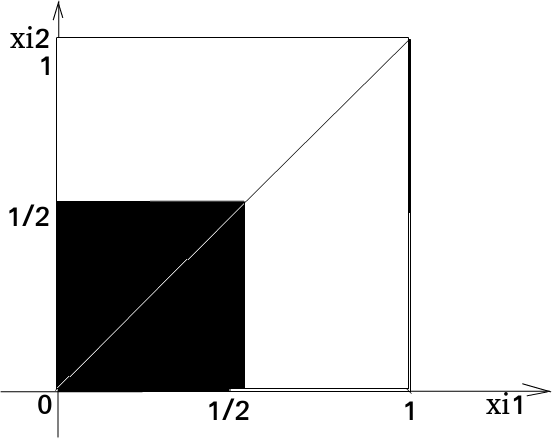
\includegraphics[width=.4\textwidth]{./pictures/5_19.png}
  \caption{Точки множества $A$}
  \label{fig:519}
\end{figure}
Вероятность пересечения событий $A$ и $B$ равна
$$P \left( A \cap B \right) =
\frac{1}{2} \cdot \frac{1}{2} =
\frac{1}{4}.$$
Тогда условная вероятность равна
$$P \left( \left. A \right| B \right) =
\frac{P \left( A \cap B \right) }{P \left( B \right) } =
\frac{ \frac{1}{4} }{ \frac{1}{2} } =
\frac{1}{2};$$
\item множество $A$ --- четвёртая часть круга с радиусом $1/2$.
Вероятность пересечения событий $A$ и $B$ равна
$$P \left( A \cap B \right) =
\frac{1}{4} \cdot \pi \left( \frac{1}{2} \right)^2 =
\frac{ \pi }{16}.$$
Тогда условная вероятность равна
$$P \left( \left. A \right| B \right) =
\frac{P \left( A \cap B \right) }{P \left( B \right) } =
\frac{ \frac{ \pi }{16} }{ \frac{1}{2} } =
\frac{ \pi }{8};$$
\item множество $A$ --- это равнобедренный прямоугольный треугольник с катетами длиной $1$.
Вероятность пересечения событий $A$ и $B$ равна
$$P \left( A \cap B \right) =
\frac{1}{4} \cdot 1^2 =
\frac{1}{4}.$$
Тогда условная вероятность равна
$$P \left( \left. A \right| B \right) =
\frac{P \left( A \cap B \right) }{P \left( B \right) } =
\frac{ \frac{1}{4} }{ \frac{1}{2} } =
\frac{1}{2}.$$
\end{enumerate}

\subsubsection*{5.20}

\textit{Задание.} Монета, для которой вероятность выпадения решки равна $p$, подбрасывается $n$ раз.
Пусть событие $A$ состоит в том, что решка выпала при первом подбрасывании, а событие $B_k$ --- в том, что выпало ровно $k$ решек.
Для каких пар $ \left( n, k \right) $ события $A$ и $B_k$ являются независимыми?

\textit{Решение.}
Опишем вероятностное пространство
$ \Omega = \\
= \left\{ \left( x_1, x_2, \dotsc, x_n \right), \,
x_i \in \left\{ 0, 1\right\}, \,
i = \overline{1, n} \right\} $,
где 1 означает, что выпала решка, 0 --- выпал орёл.
На каждом месте может стоять либо единица, либо ноль.
Поэтому $ \left| \Omega \right| =2^n$.

Опишем событие $A = \left\{ \left( x_1, x_2, \dotsc, x_n \right) \in \Omega, \, x_1 = 1 \right\} $.
На первом месте может стоять только единица.
Количество способов её выбрать равно одному.
Тогда остаётся посчитать, сколько есть вариантов выпадения монеты при остальных $n - 1$ подбрасываниях.
Имеем $ \left| A \right| = 2^{n-1} p \cdot \sum \limits_{i=1}^{n-1} \left( 1-p \right)^i p^{n-i}$.
Тогда вероятность события $A$ равна
$$P \left( A \right) =
\frac{2^{n-1} p \cdot \sum \limits_{i=1}^{n-1} \left( 1-p \right)^i p^{n-i}}{2^n} =
\frac{p \cdot \sum \limits_{i=1}^{n-1} \left( 1-p \right)^i p^{n-i}}{2}.$$

Опишем событие $B_k = \left\{ \left( x_1, x_2, \dotsc, x_n \right) \in \Omega, \, \sum \limits_{i=1}^k x_i = k \right\} $.
На $k$ местах могут стоять только единицы, на остальных $n - k$ местах --- только нули.
Найдём количество способов выбрать $k$ мест, где будут единицы.
Это $C_n^k p^k \left( 1-p \right)^{n-k}$.
Тогда вероятность равна
$$P \left( B_k \right) =
\frac{C_n^k p^k \left( 1-p \right)^{n-k}}{2^n}.$$

Чтобы события были независимы, нужно, чтобы вероятность пересечения этих событий равнялась произведению их вероятностей.
Найдём произведение вероятностей:
\begin{equation*}
\begin{split}
P \left( A \right) P \left( B_k \right) =
\frac{p \cdot \sum \limits_{i=1}^{n-1} \left( 1-p \right)^i p^{n-i}}{2} \cdot \frac{C_n^k p^k \left( 1-p \right)^{n-k}}{2^n} = \\
= \frac{p p^k \left( 1-p \right)^{n-k} C_n^k \cdot \sum \limits_{i=1}^{n-1} p^{n-i} \left( 1-p \right)^i}{2^{n+1}} = \\
= \frac{p^{k+1} \left( 1-p \right)^{n-k} C_n^k \cdot \sum \limits_{i=1}^{n-1} p^{n-i} \left( 1-p \right)^i}{2^{n+1}}.
\end{split}
\end{equation*}

Найдём вероятность переечения этих событий:
$$P \left( A \cap B \right) =
P \left( \left\{ \left( x_1, x_2, \dotsc, x_n \right) \in \Omega, \, \sum \limits_{i=1}^k x_i = k, \, x_1 = 1 \right\} \right).$$
Нужно выбрать $k - 1$ место, где будут единицы.
Тогда
$$P \left( A \cap B \right) =
\frac{p^k \left( 1-p \right)^{n-k} C_n^{k-1}}{2^n}.$$

Приравняем полученные результаты:
$$ \frac{p^{k+1} \left( 1-p \right)^{n-k} C_n^k \cdot \sum \limits_{i=1}^{n-1} p^{n-i} \left( 1-p \right)^i}{2^{n+1}} =
\frac{p^k \left( 1-p \right)^{n-k} C_n^{k-1}}{2^n}.$$
Сократим на
$$\frac{p^k \left( 1-p \right)^{n-k}}{2^n}.$$
Получим:
$$ \frac{p C_n^k \cdot \sum \limits_{i=1}^{n-1} p^{n-i} \left( 1-p \right)^i}{2} =
C_n^{k-1}.$$
Распишем:
$$ \frac{p \cdot \sum \limits_{i=1}^{n-1} p^{n-i} \cdot n!}{2k! \left( n-k \right)!} =
\frac{n!}{ \left( k-1 \right)! \left( n-k+1 \right)!}.$$
Сократим на $n!$ и внесём $p$ под знак суммы:
$$\frac{\sum \limits_{i=1}^{n-1} p^{n-i+1}}{2k! \left( n-k \right)!} = \frac{1}{ \left( k-1 \right)! \left( n-k+1 \right)!}.$$
Распишем факториалы:
$$\frac{\sum \limits_{i=1}^{n-1} p^{n-i+1}}{2 \left( k-1 \right)!k \left( n-k \right)!} = \frac{1}{ \left( k-1 \right)! \left( n-k \right)! \left(n-k+1 \right)!}.$$
Сократим:
$$\frac{\sum \limits_{i=1}^{n-1} p^{n-i+1}}{2k} = \frac{1}{n-k+1}.$$

\subsubsection*{5.21}

\textit{Задание.} Вероятность безотказной работы реле при перегреве равна $0.95$, при вибрации --- $0.9$, при перегреве и вибрации --- $0.8$.
Найдите вероятность отказа реле, если вероятность перегрева равна $0.2$, вероятность вибрации --- $0.1$, и считая, что перегрев и вибрация являются независимыми событиями.

\textit{Решение.}
Пусть событие $A =$ \{реле перегрелось\}, событие $B =$ \{произошла вибрация\}, событие $C =$ \{произошёл отказ реле\}, такие что
\begin{equation*}
\begin{split}
P \left( A \right) = 0.2, \,
P \left( B \right) = 0.1, \,
P \left( \left. \overline{C} \right| A \right) = 0.95, \,
P \left( \left. \overline{C} \right| B \right) = 0.9, \\
P \left( \left. \overline{C} \right| A \cap B \right) = 0.2.
\end{split}
\end{equation*}

Распишем условную вероятность:
$$P \left( \left. \overline{C} \right| A \right) =
\frac{P \left( \overline{C} \cap A \right) }{P \left( A \right) } =
\frac{P \left( \overline{C} \cap A \right) }{0.2} =
0.95.$$
Отсюда $P \left( \overline{C} \cap A \right) = 0.2 \cdot 0.95 = 0.19$.

Распишем условную вероятность:
$$P \left( \left. \overline{C} \right| B \right) =
\frac{P \left( \overline{C} \cap B \right) }{P \left( B \right) } =
\frac{P \left( \overline{C} \cap B \right) }{0.1} =
0.9.$$
Отсюда $P \left( \overline{C} \cap B \right) = 0.1 \cdot 0.9 = 0.09$.

Распишем условную вероятность:
\begin{equation*}
\begin{split}
P \left( \left. \overline{C} \right| A \cap B \right) =
\frac{P \left( \overline{C} \cap A \cap B \right) }{P \left( A \cap B \right) } =
\frac{P \left( \overline{C} \cap A \cap B \right) }{P \left( A \right) P \left( B \right) } =
\frac{P \left( \overline{C} \cap A \cap B \right) }{0.2 \cdot 0.1} = \\
= \frac{P \left( \overline{C} \cap A \cap B \right) }{0.02} =
0.2.
\end{split}
\end{equation*}
Отсюда $P \left( \overline{C} \cap A \cap B \right) = 0.2 \cdot 0.02 = 0.004$.

Посчитаем
$P \left( \overline{ \overline{C} \cap A} \right) =
P \left( C \cup \overline{A} \right) =
P \left( C \right) + P \left( \overline{A} \right) - P \left( C \cap \overline{A} \right) =
P \left( C \right) + \\
+ 1 - 0.2 - P \left( C \cap \overline{A} \right) =
1 - 0.19$.
Тогда $P \left( C \right) - P \left( C \cap \overline{A} \right) = 0.2 - 0.19 = 0.01$.

Найдём
$P \left( \overline{ \overline{C} \cap B} \right) =
P \left( C \cup \overline{B} \right) =
P \left( C \right) + P \left( \overline{B} \right) - P \left( C \cap \overline{B} \right) =
P \left( C \right) + \\ + 1 - 0.1 - P \left( C \cap \overline{B} \right) =
1 - 0.09.$
Отсюда $P \left( C \right) - P \left( C \cap \overline{B} \right) = 0.1 - 0.09 = 0.01$.

Найдём
$P \left( \overline{ \overline{C} \cap A \cap B} \right) =
P \left( C \cup \overline{A} \cup \overline{B} \right) =
P \left( C \right) + P \left( \overline{A} \right) + P \left( \overline{B} \right) - \\
- P \left( C \cap \overline{A} \right) - P \left( C \cap \overline{B} \right) - P \left( \overline{A} \cap \overline{B} \right) +
P \left( C \cap \overline{A} \cap \overline{B} \right) =
P \left( C \right) + 1 - 0.2 + 1 - \\ 
- 0.1 - P \left( C \cap \overline{A} \right) - P \left( C \cap \overline{B} \right) - \left( 1 - 0.2 \right) \left( 1 - 0.1 \right) +
P \left( C \cap \overline{A} \cap \overline{B} \right) =
P \left( C \right) - \\
- P \left( C \cap \overline{A} \right) -
P \left( C \cap \overline{B} \right) +P \left( C \cap \overline{A} \cap \overline{B} \right) + 0.98 =
1 - 0.004 =
0.996$.
Отсюда
$P \left( C \right) -
P \left( C \cap \overline{A} \right) -
P \left( C \cap \overline{B} \right) + P \left( C \cap \overline{A} \cap \overline{B} \right) = 0.016$.

Составим систему:
\begin{equation*}
\begin{split}
\begin{cases}
P \left( C \right) = P \left( C \cap \overline{A} \right) + 0.01; \\
P \left( C \right) = P \left( C \cap \overline{B} \right) + 0.01; \\
P \left( C \right) =
P \left( C \cap \overline{B} \right) -  P \left( C \cap \overline{A} \cap \overline{B} \right) + P \left( C \cap \overline{A} \right) + 0.016.
\end{cases}
\end{split}
\end{equation*}

Получили 3 уравнения и 4 неизвестных.
Упростим:
$P \left( C \right) =
P \left( C \right) - \\
- 0.01 - P \left( C \cap \overline{A} \cap \overline{B} \right) + P \left( C \right) - 0.01 + 0.016 =
0.006 - P \left( C \cap \overline{A} \cap \overline{B} \right) + 2P \left( C \right) $.

Выразим вероятность события $C$.
Получим:
$P \left( C \right) = 0.012 - \\
- 0.5 P \left( C \cap \overline{A} \cap \overline{B} \right) $.

Отсюда $P \left( C \cap \overline{A} \cap \overline{B} \right) = 0.024 - 2 P \left( C \right) $.

По формуле включений-исключений:
$P \left( \overline{C \cap \overline{A} \cap \overline{B}} \right) =
P \left( \overline{C} \cup A \cup B \right) = \\
= P \left( \overline{C} \right) +
P \left( A \right) +
P \left( B \right) -
P \left( \overline{C} \cap A \right) -
P \left( \overline{C} \cap B \right) - P \left( A \cap B \right) + P \left( \overline{C} \cap A \cap B \right) = \\
= 1 - P \left( C \right) + 0.2 + 0.1 - 0.2 \cdot 0.1 + 0.04 =
0.92 - P \left( C \right) $.

Это равно $0.92 - P \left( C \right) = 1 - P \left( C \cap \overline{A} \overline{B} \right) = 1 - 0.024 + 2 P \left( C \right) $.
Тогда $0.92 - P \left( C \right) = 0.076 + 2 P \left( C \right) $.
Выразим вероятность события $C$ из этого уравнения: $3P \left( C \right) = 0.92 - 0.076 = 0.844$.
Отсюда $P \left( C \right) = 0.844/3 = \\ = 0.281 \left( 3 \right) $.

\subsubsection*{5.22}

\textit{Задание.} Вероятность того, что сервер будет атакован на протяжении дня равна $0.1$.
Считая, что в разные дни атаки происходят независимо, найти вероятность того, что за неделю сервер:
\begin{enumerate}[label=\alph*)]
\item будет атакован 2 раза;
\item не будет атакован.
\end{enumerate}

\textit{Решение.}
\begin{enumerate}[label=\alph*)]
\item За неделю сервер будет атакован 2 раза и в остальные 5 дней не будет атакован.
Нужно выбрать 2 дня из семи, когда сервер будет атакован --- это $C_7^2$.
Тогда вероятность того, что сервер будет атакован ровно 2 раза за неделю, равна
$P =
C_7^2 \cdot \left( 0.1 \right)^2 \left( 1 - 0.1 \right)^5$; 
\item вероятность того, что север не будет атакован ни разу за неделю, равна $P = \left( 1 - 0.1 \right)^7$.
\end{enumerate}

\subsubsection*{5.23}

\textit{Задание.} Пусть событие $R_i$ состоит в том, что $i$-ый игрок в покер имеет на руках <<royal flush>> (то есть 10, В, Д, К, Т одной масти).
Покажите, что наличие одного <<royal flush>> увеличивает вероятность второго <<royal flush>>, то есть
$P \left( \left. R_2 \right| R_1 \right) >
P \left( R_2 \right) $.

\textit{Решение.} Распишем условную вероятность
$$P \left( \left. R_2 \right| R_1 \right) =
\frac{P \left( R_2 \cap R_1 \right) }{P \left( R_1 \right) }.$$
Нужно доказать, что $P \left( R_2 \cap R_1 \right) > P \left( R_2 \right) P \left( R_1 \right) $.

Найдём вероятность того, что у первого игрока будет на руках <<royal flush>>.
Выберем одну масть из четырёх: $C_4^1$.
Вероятность сочетания равна
$$P \left( R_1 \right) =
\frac{C_4^1}{C_{52}^5}.$$

Найдём вероятность того, что у двух игроков появится <<royal flush>>.
Сначала выберем данное сочетание карт одной масти.
Остаётся 3 масти.
Выбрать одну из них можно $C_3^1$ способом.
Тогда вероятность равна
$$P \left( R_1 \cap R_2 \right) =
\frac{C_4^1C_3^1}{C_{52}^{10}} =
\frac{4 \cdot 3 \cdot 10! \cdot 42!}{52!} =
\frac{12 \cdot 10! \cdot 42!}{52!}.$$

Распишем произведение вероятностей:
$$P \left(R_1 \right) P \left( R_2 \right) =
\left( \frac{C_4^1}{C_{52}^{5}} \right)^2 =
\left( \frac{4 \cdot 5! \cdot 47!}{52!}\right)^2 =
\frac{16 \cdot 5! \cdot 5! \cdot 47! \cdot 47!}{52! \cdot 52!}.$$

Нужно показать, что
$$\frac{12 \cdot 10! \cdot 42!}{52!} >
\frac{16 \cdot 5! \cdot 5! \cdot 47! \cdot 47!}{52! \cdot 52!}.$$
Сократим на
$$ \frac{4}{52!}$$
и распишем факториалы:
$$3 \cdot 5! \cdot 5 \cdot 7 \cdot 8 \cdot 9 \cdot 42! >
\frac{4 \cdot 5! \cdot 2 \cdot 3 \cdot 4 \cdot 5 \cdot 42! \cdot 43 \cdot 44 \cdot 45 \cdot 46 \cdot 47 \cdot 47!}{52!}.$$

Сократим на $3 \cdot 5 \cdot 5! \cdot 42!$, а также сократим дробь на $47!$.
Получим:
$$7 \cdot 8 \cdot 9 >
\frac{4 \cdot 2 \cdot 4 \cdot 43 \cdot 44 \cdot 45 \cdot 46 \cdot 47}{48 \cdot 49 \cdot 50 \cdot 51 \cdot 52} =
\frac{32 \cdot 43 \cdot 44 \cdot 45 \cdot 46 \cdot 47}{48 \cdot 49 \cdot 50 \cdot 51 \cdot 52}.$$
Получили, что дробь справа --- это $32$, умноженное на число меньше единицы.
Это число не будет превышать 32.
А слева --- $504 > 32$.
Неравенство доказано.

\subsubsection*{5.24}

\textit{Задание.} Монета находится в одном из $n$ ящиков.
Вероятность того, что она в $i$-м ящике равна $p_i$.
Если вы будете искать монету в $i$-м ящике и она действительно там, вы найдёте её с вероятностью $a_i$.
Покажите, что вероятность $p$ того, что монета находится в $j$-м ящике, при условии, что вы искали и не нашли её в $i$-м ящике, равна
\begin{equation*}
\begin{split}
p =
\begin{cases}
\frac{p_j}{1-p_i a_i}, i \neq j, \\
\frac{ \left( 1-a_i \right) p_i}{1-p_i a_i}, i = j.
\end{cases}
\end{split}
\end{equation*}

\textit{Решение.} Пусть Событие $B = $ \{монета находится в $j$-м ящике\}.
Его вероятность равна $P \left( B \right) = p_i$.
Событие $A =$ \{находим монету в $i$-м ящике\}, т.е. мы её ищем, находим, монета там лежит.
Его вероятность равна $P \left( A \right) = \\ = p_i a_i$.

Пусть $i \neq j$.
Вероятность пересечения событий $ \overline{A}$ и $B$ означает, что монета находится в каком-то $j$-м ящике.
Тогда условная вероятность события $B$ при условии, что произошло событие $ \overline{A}$, равна
$$P \left( \left. B \right| \overline{A} \right) =
\frac{P \left( \overline{A} \cap B \right) }{P \left( \overline{A} \right) } =
\frac{p_j}{1-p_i a_i}.$$

Рассмотрим случай, когда $i = j$.
Тогда мы не находим её в $i$-м ящике, но она там находится.
Вероятностьь в этом случае равна
$$p =
\frac{ \left( 1-a_i \right) p_i}{1-p_i a_i}.$$

\subsubsection*{5.25}

\textit{Задание.} Допустим, что $A$ и $B$ такие события, что
$P \left( \left. A \right| B \right) = P \left( \left. B \right| A \right); \,
P \left( A \cup B \right) = \\
= 1; \,
P \left( A \cap B \right) > 0$.
Докажите, что $P \left( A \right) > 1/2$.

\textit{Решение.} Распишем условные вероятности:
$$P \left( \left. A \right| B \right) =
\frac{P \left( A \cap B \right) }{P \left( B \right) }.$$
По условию задачи это равно
$$P \left( \left. B \right| A \right) =
\frac{P \left( A \cap B \right) }{P \left( B \right) }.$$
Отсюда видим, что $P \left( A \right) = P \left( B \right) $.

По формуле включений-исключений:
$P \left( A \cup B \right) =
P \left( A \right) + P \left( B \right) - P \left( A \cap B \right) = \\
= 2P \left( A \right) - P \left( A \cap B \right) =
1$.
Выразим отсюда вероятность события $A$.
Имеем:
$$P \left( A \right) = \frac{1}{2} + \frac{P \left( A \cap B \right) }{2}.$$
По условию $P \left( A \cap B \right) > 0$.
Поэтому
$$P \left( A \right) >
\frac{1}{2}.$$

\subsubsection*{5.26}

\textit{Задание.} Пусть события $A$ и $B$ независимые и $A \subset B$.
Докажите, что или $P \left( A \right) = 0$, или $P \left( B \right) = 1$.

\textit{Решение.} Так как события независимы, то справедлива формула $P \left( A \cap B \right) =  \\ = P \left( A \right) P \left( B \right) $.
Так как $A \subset B$, то $A \cap B = A$.
Поэтому $P \left( A \cap B \right) = P \left( A \right) = \\ = P \left( A \right) P \left( B \right) $.

Если $P \left( A \right) \neq 0$, то можно на него сократить, тогда $P \left( B \right) = 1$.
Иначе $P \left( A \right) = 0$, тогда $P \left( B \right) \in \left( 0, 1 \right) $.

\subsubsection*{5.27}

\textit{Задание.} Докажите, что
$P \left( \left. A_1 \dotsc A_n \right| C \right) =
P \left( \left. A_1 \right| C \right)
P \left( \left. A_2 \right| A_1 C \right) \dotsc \cdot \\
\cdot P \left( \left. A_n \right| A_1 A_2 \dotsc A_{n-1} C \right) $.

\textit{Решение.} Распишем левую часть:
$$P \left( \left. A_1 \dotsc A_n \right| C \right) =
\frac{P \left( A_1 \dotsc A_n C \right) }{P \left( C \right) }.$$
Распишем правую часть:
\begin{equation*}
\begin{split}
P \left( \left. A_1 \right| C \right) P \left( \left. A_2 \right| A_1 C \right) \dotsc
P \left( \left. A_n \right| A_1 A_2 \dotsc A_{n-1} C \right) = \\
= \frac{P \left( A_1 C \right) }{P \left( C \right) } \cdot \frac{P \left( A_1 A_2 C \right) }{P \left( A_1 C \right) } \dotsc
\frac{P \left( A_1 A_2 \dotsc A_{n-1} A_n C \right) }{P \left( A_1 A_2 \dotsc A_{n-1} C \right) }.
\end{split}
\end{equation*}
Всё кроме числителя последней дроби и знаменателя первой дроби сокращается.
Получаем то, что требовали:
$$P \left( \left. A_1 \right| C \right) P \left( \left. A_2 \right| A_1 C \right) \dotsc
P \left( \left. A_n \right| A_1 A_2 \dotsc A_{n-1} C \right) =
\frac{P \left( A_1 A_2 \dotsc A_{n-1} A_n C \right) }{P \left( C \right) }.$$
А это равно левой части.

\subsubsection*{5.28}

\textit{Задание.} Пусть событие $A$ такое, что $P \left( A \right) $ равно 0 или 1.
Докажите, что $A$ и произвольное событие $B$ независимы.

\textit{Решение.} $A$ может быть либо пустым множеством, либо совпадать с множеством элементарных исходов.

Пусть $A = \varnothing$.
Тогда $P \left( A \right) = 0$.
Рассмотрим произведение вероятностей события $A$ и произвольного события $B$.
Оно равно $P \left( A \right) P \left( B \right) = 0 \cdot P \left( B \right) = \\ = 0$.
Рассмотрим вероятность пересечения событий: $P \left( A \cap B \right) = P \left( \varnothing \cap B \right) = \\ = P \left( \varnothing \right) = 0$.
События называются независимыми, если $P \left( A \cap B \right) = P \left( A \right) P \left( B \right) $.
Получили, что это равенство выполняется, значит события независимы.

Если $A = \Omega $, то $P \left( A \right) = 1$.
Рассмотрим произведение вероятностей события $A$ и произвольного события $B$.
Оно равно $P \left( A \right) P \left( B \right) = 1 \cdot P \left( B \right) = \\ = P \left( B \right)$.
Рассмотрим вероятность пересечения событий: $P \left( A \cap B \right) = P \left( \Omega \cap B \right) = \\ = P \left( B \right) $.
События независимы, так как $P \left( A \cap B \right) = P \left( A \right) P \left( B \right) $.

\addcontentsline{toc}{chapter}{Занятие 6. Формула полной вероятности. Формула Байеса}
\chapter*{Занятие 6. Формула полной вероятности. Формула Байеса}

\addcontentsline{toc}{section}{Контрольные вопросы и задания}
\section*{Контрольные вопросы и задания}

\subsubsection*{Приведите определение полной группы гипотез.}

Набор случайных событий $H_1, \dotsc, H_n$ называется полным набором гипотез, если выполнены следующие условия:
\begin{enumerate}
\item $P \left( H_i \right) > 0, \, i = \overline{1, n} $;
\item $H_i \cap H_j = \varnothing, \, i \neq j$ (они несовместны);
\item $ \bigcup \limits_{i=1}^n H_i = \Omega $.
\end{enumerate}

\subsubsection*{Запишите формулу для вычисления условной вероятности, формулу полной вероятности, формулу Байеса.}

Условная вероятность события $A$ при условии, что событие $B$ произошло --- это выражение
$$P \left( \left. A \right| B \right) =
\frac{P \left( A \cap B \right) }{P \left( B \right) }.$$

Формула полной вероятности: $P \left( A \right) = \sum \limits_{i=1}^n P \left( \left. A \right| H_i \right) P \left( H_i \right) $.

Формула Байеса:
$$P \left( \left. H_i \right| A \right) =
\frac{P \left( \left. A \right| H_i \right) P \left( H_i \right) }{ \sum \limits_{k=1}^n P \left( \left. A \right| H_k \right) P \left( H_k \right) }.$$

\addcontentsline{toc}{section}{Домашнее задание}
\section*{Домашнее задание}

\subsubsection*{6.13}

\textit{Задание.} В первой урне содержатся 1 белый и 9 чёрных шаров; во второй урне --- 1 чёрный и 5 белых шаров.
Из каждой урны наугад вынуто по одному шару, а остальные пересыпали в третью урну.
Найдите вероятность того, что шар, вынятый наугад из третьей урны, окажется белым.

\textit{Решение.}
Введём полную группу событий:
$H_1 =$ \{в третью урну переложили 10 чёрных и 4 белых шара\} = \{из обеих урн вынули по одному белому шару\};
$H_2 =$ \{в третью урну переложили 9 чёрных и 5 белых шаров\} = \{из одной урны достали 1 белый шар, и из второй --- 1 чёрный шар\};
$H_3 =$ \{в третью урну переложили 8 чёрных и 6 белых шаров\} = \{из обеих урн вынули по одному чёрному шару\}.
Определим вероятности этих событий:
\begin{equation*}
\begin{split}
P \left\{ H_1 \right\} =
\frac{1}{10} \cdot \frac{5}{6} =
\frac{1}{12}, \,
P \left\{ H_2 \right\} =
\frac{1}{10} \cdot \frac{1}{6} + \frac{9}{10} \cdot \frac{5}{6} =
\frac{1}{60} + \frac{3}{4} =
\frac{1+15}{60} =
\frac{16}{60} = \\
= \frac{1}{5}, \,
P \left\{ H_3 \right\} =
\frac{9}{10} \cdot \frac{1}{6} =
\frac{3}{10 \cdot 2} =
\frac{3}{20}.
\end{split}
\end{equation*}
Введём событие $A =$ \{из третьей урны вытянули белый шар\}.
В то же время
$$P \left\{ \left. A \right| H_1 \right\} =
\frac{4}{14} =
\frac{2}{12}, \,
P \left\{ \left. A \right| H_2 \right\} =
\frac{5}{14}, \,
P \left\{ \left. A \right| H_3 \right\} =
\frac{6}{14} =
\frac{3}{7}.$$
Согласно с формулой полной вероятности $P \left\{ A \right\} = \sum \limits_{i=1}^\infty P \left\{ H_i \right\} \cdot P \left\{ \left. A \right| H_i \right\} $ имеем
\begin{equation*}
\begin{split}
P \left\{ A \right\} =
\frac{1}{12} \cdot \frac{2}{12} + \frac{1}{5} \cdot \frac{5}{14} + \frac{3}{20} + \frac{3}{7} =
\frac{1}{72} + \frac{1}{14} + \frac{9}{140} =
\frac{1960+10080+9072}{141120} = \\
= \frac{21112}{141120}=
\frac{377}{2520}.
\end{split}
\end{equation*}

\subsubsection*{6.14}

\textit{Задание.} Два стрелка стреляют по мишени.
Один из них попадает в 5 случаях, а другой --- в 8 случаях из 10.
Перед выстрелом они подбрасывают правильную монету для определения очередности.
Сторонний наблюдатель знает условия стрельбы, но не видит, кто в данный момент стреляет.
Он видит, что стрелок попал по мишени.
Найдите вероятность того, что стрелял первый стрелок.

\textit{Решение.} Первый стрелок попадает по мишени с вероятностью
$$P \left( \left. A \right| H_1 \right) =
\frac{5}{10} =
\frac{1}{2},$$
второй стрелок --- с вероятностью
$$P \left( \left. A \right| H_2 \right) =
\frac{8}{10} =
\frac{4}{5}.$$
Априорные вероятности этих гипотез одинаковы:
$$P \left( H_1 \right) =
P \left( H_2 \right) =
\frac{1}{2}.$$
Рассмотрим событие $A =$ \{стрелок попал в цель\}.
Поэтому вероятность стрелять первому стрелку
\begin{equation*}
\begin{split}
P \left( \left. A \right| H_1 \right) =
\frac{P \left( \left. A \right| H_1 \right) P \left( H_1 \right) }{P \left( \left. A \right| H_1 \right) P \left( H_1 \right) +
P \left( \left. A \right| H_2 \right) P \left( H_2 \right) } =
\frac{ \frac{1}{2} \cdot \frac{1}{2} }{ \frac{1}{2} \cdot \frac{1}{2} + \frac{4}{5} \cdot \frac{1}{2} } =
\frac{ \frac{1}{4} }{ \frac{1}{4} + \frac{2}{5} } = \\
= \frac{ \frac{1}{4} }{ \frac{5+8}{20} } =
\frac{20}{4 \cdot 13} =
\frac{5}{13}.
\end{split}
\end{equation*}

\addcontentsline{toc}{chapter}{Контрольная работа 1}
\chapter*{Контрольная работа 1}

\addcontentsline{toc}{section}{Вариант 1}
\section*{Вариант 1}

\subsubsection*{1}

\textit{Задание.} В сундуке лежат 10 красных, 6 синих и 4 зелёных пуговицы.
Найдите вероятность того, что две наугад вынутые пуговицы будут разного цвета.

\textit{Решение.}
Опишем пространство элементарных исходов: $ \Omega = \\ = \left\{ \left( x, y \right), \, x, y \in \right.$ красный, синий, зелёный\}\}.
Нужно выбрать две пуговицы из двадцати, поэтому $ \left| \Omega \right| = C_{20}^2$.

Опишем событие $A =$ \{две наугад вынутые пуговицы будут разного цвета\} $= \left\{ \left( x, y \right) in \Omega: \, x \neq y \right\} $.
Выберем сначала одну красную пуговицу --- $C_{10}^1$, а затем --- одну синюю --- $C_6^1$.
По правилу умножения есть $C_{10}^1 \cdot C_6^1$ способов вынуть одну красную и одну синюю пуговицу.
Второй случай: одна из пуговиц красная, другая --- зелёная --- $C_{10}^1 \cdot C_4^1$.
Третий случай: одна из пуговиц синяя, другая --- зелёная --- $C_6^1 \cdot C_4^1$.
По правилу суммы имеем, что $ \left| A \right| = C_{10}^1 \cdot C_6^1 + C_{10}^1 \cdot C_4^1 + C_6^1 \cdot C_4^1$.

Тогда вероятность равна
$$P \left( A \right) =
\frac{ \left| A \right| }{ \left| \Omega \right| } =
\frac{C_{10}^1 \cdot C_6^1 + C_{10}^1 \cdot C_4^1 + C_6^1 \cdot C_4^1}{C_{20}^2}.$$

\subsubsection*{2}

\textit{Задание.} Подбросили 10 игральных кубиков.
Найдите вероятность того, что единица выпала хотя бы на двух кубиках, если известно, что она выпала хотя бы на одном кубике.

\textit{Решение.}
Опишем пространство элементарных событий:
$ \Omega = \\
= \left\{ \left( x_1, x_2, \dotsc, x_{10} \right): \,
x_i \in \left\{1, 2, 3, 4, 5, 6 \right\}, \,
i =
\overline{1, 6} \right\} $.
На каждом кубике может выпасть число от одного до шести (6 вариантов), поэтому $ \left| \Omega \right| = 6^{10}$.

Рассмотрим событие $A =$ \{единица не выпала ни на одном кубике\}.
На каждом кубике может выпасть число от одного до пяти.
Таких вариантов есть $5^{10}$.
Тогда вероятность события $A$ равна
$$P \left( A \right) =
\frac{ \left| A \right| }{ \left| \Omega \right| } =
\frac{5^{10}}{6^{10}}.$$

Тогда событие $ \overline{A} =$ \{единица выпала хотя бы на одном кубике\} имеем вероятность
$$P \left( \overline{A} \right) =
1 - P \left( A \right) =
1 - \frac{5^{10}}{6^{10}}.$$

Рассмотрим событие $B =$ \{единица выпала хотя бы на двух кубиках\}.
Рассмотрим пересечение событий $ \overline{A} \cap B =$ \{единица выпала хотя бы на двух кубиках\} $= B$.
Рассмотрим противоположное событие: $ \overline{B} =$ \{единица выпала ровно на одном кубике\} $
\cup $ \{единица не выпала ни на одном кубике\} $= B_1 \cup A$.
Найдём количество способов выпадения цифр на кубиках, которые ему удовлетворяют.

$B_1 =$ \{единица выпала ровно на одном кубике\}.
Нужно выбрать 1 кубик из десяти, на котором выпала единица --- это $C_{10}^1$.
На остальных десяти кубиках может быть любое число от двух до шести --- $5^9$.
По правилу умножения $ \left| B_1 \right| = C_{10}^1 \cdot 5^9$.
Вероятность этого события равна
$$P \left( B_1 \right) =
\frac{ \left| B_1 \right) }{ \left| \Omega \right| } =
\frac{C_{10}^1 \cdot 5^9}{6^{10}}.$$

Тогда вероятность события $B$ равна
$$P \left( B \right) =
P \left( A \right) + P \left( B_1 \right) =
\frac{5^{10}}{6^{10}} + \frac{C_{10}^1 \cdot 5^9}{6^{10}} =
\frac{5^{10} + C_{10}^1 \cdot 5^9}{6^{10}}.$$

Условная вероятность события $B$ при условии, что событие $ \overline{A}$ произошло, равна
$$P \left( \left. B \right| \overline{A} \right) =
\frac{P \left( \overline{A} \cap B \right)}{P \left( \overline{A} \right) } =
\frac{P \left( B \right)}{P \left( \overline{A} \right) } =
\frac{ \frac{5^{10} + C_{10}^1 \cdot 5^9}{6^{10}}}{1 - \frac{5^{10}}{6^{10}} }.$$

\subsubsection*{3}

\textit{Задание.} Допустим, что в среднем 5 мужчин из 100 и 25 женщин из 10000 являются дальтониками.
Наугад выбранный человек оказался дальтоником.
Какая вероятность того, что это был мужчина?

\textit{Решение.} Рассмотрим событие $A =$ \{наугад быбранный человек оказался дальтоником\}.
Рассмотрим гипотезы: $H_1 =$ \{выбранный человек --- мужчина\}, $H_2 =$ \{выбранный человек --- женщина\}.
Мужчин и женщин в популяции одинаковое количество, поэтому вероятности гипотез равны
$$P \left( H_1 \right) =
\frac{1}{2} =
P \left( H_2 \right).$$
Условные вероятности:
$$P \left( \left. A \right| H_1 \right) =
\frac{5}{100}, \,
P \left( \left. A \right| H_2 \right) =
\frac{25}{10000}.$$
По формуле Байеса
$$P \left( \left. H_1 \right| A \right) =
\frac{P \left( \left. A \right| H_1 \right) P \left( H_1 \right) }{P \left( \left. A \right| H_1 \right) P \left( H_1 \right) +
P \left( \left. A \right| H_2 \right) P \left( H_2 \right) } =
\frac{ \frac{5}{100} \cdot \frac{1}{2} }{ \frac{5}{100} \cdot \frac{1}{2} +  \frac{25}{10000} \cdot \frac{1}{2} }.$$

\subsubsection*{4}

\textit{Задание.} Петя играет в орлянку.
Он начинает игру, имея одну гривну.
Если выпадет орёл, то Петя получает одну гравну, в другом случае --- теряет одну гривну.
Была сиграна 21 игра, после которой Петя остался без денег и без долга.
Найдите вероятность того, что Петя впервые остался без денег именно в последней игре.

\textit{Решение.} На рисунке \ref{fig:14} изображены возможные пути.

\begin{figure}[h!]
  \centering
  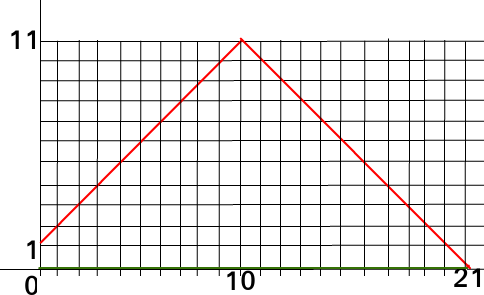
\includegraphics[width=.4\textwidth]{./pictures/t1v1_4.png}
  \caption{Пути}
  \label{fig:14}
\end{figure}

Они ограничиваются красной линией.
Зелёную линию пересекать не можем.
Касаться её можно только в точке $ \left( 21, 0 \right) $.

Перевернём изображение (рис. \ref{fig:1	41}).

\begin{figure}[h!]
  \centering
  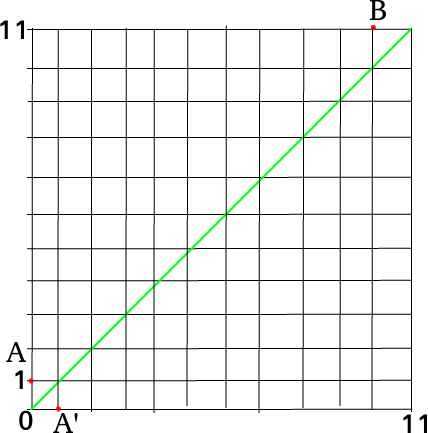
\includegraphics[width=.4\textwidth]{./pictures/t1v1_41.png}
  \caption{Перевёрнутое изображение}
  \label{fig:141}
\end{figure}

Теперь можем ходить направо и вверх.
Всего путей из точки $A$ (начальной) в точку $B$ (конечную) $C_{10+11}^{10} = C_{21}^{10}$.
По методу отражения путей, которые касаются или пересекают диагональ столько, сколько путей из точки $A'$ в точку $B$.
Их $C_{9+11}^9 = C_{20}^9$.
Тогда путей, которые не касаются и не пересекают диагональ $C_{21}^{10} - C_{20}^9$.

А вероятность такого события равна
$$P =
\frac{C_{21}^{10} - C_{20}^9}{C_{21}^{10}}.$$

\subsubsection*{5}

\textit{Задание.} В равнобедренный прямоугольный треугольник с катетами длиной $1$ см наугад бросили точку.
Найдите вероятность того, что расстояние от этой точки до какой-то из вершин треугольника не превышает 0.5 см.

\textit{Решение.} Эта задача на геометрическую вероятность.
Пространство элементарных событий $ \Omega $ --- равнобедренный прямоугольный треугольник с катетами длиной 1.
Его площадь равна
$$S_{ \Omega } =
\frac{1}{2} \cdot 1 \cdot 1 =
\frac{1}{2}.$$
Событие $A =$ \{расстояние от наугад выбранной точки в данном треугольнике до какой-то из его вершин не превышает 0.5\} на рисунке \ref{fig:5} закрашено чёрным цветом.

\begin{figure}[h!]
  \centering
  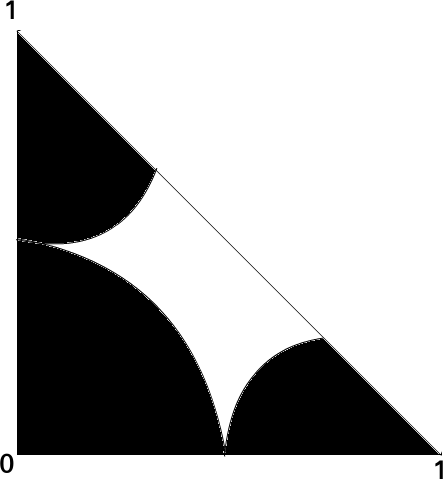
\includegraphics[width=.4\textwidth]{./pictures/t1v1_5.png}
  \caption{Пространство элементарных событий $ \Omega $ и событие $A$}
  \label{fig:5}
\end{figure}

Точки множества $A$ образуют 3 части.
Первая часть --- четверть круга с радиусом 0.5 возле прямого угла.
Его площадь равна
$$S_1 =
\frac{1}{4} \cdot \pi \left( \frac{1}{2} \right)^2 =
\frac{ \pi }{16}.$$

Две остальные части равна.
Их площади можно найти по формуле для площади сектора круга.
Треугольник равнобедренный и прямоугольный, поэтому углы равны $45 \degree$.
Тогда
$$S_2 =
S_3 =
\frac{ \pi \cdot  \left( \frac{1}{2} \right)^2 \cdot \frac{ \pi }{4}}{2 \pi } =
\frac{ \pi }{16 \cdot 2}.$$

Тогда
$$S_A =
S_1 + S_2 + S_3 =
\frac{ \pi }{16} + 2 \cdot \frac{ \pi }{16 \cdot 2} =
\frac{ \pi }{16} + \frac{ \pi }{16} =
\frac{ \pi }{8}.$$

Вероятность этого события равна
$$P \left( A \right) =
\frac{S_A}{S_{ \Omega }} =
\frac{ \frac{ \pi }{8} }{ \frac{1}{2} } =
\frac{ \pi }{4}.$$

\addcontentsline{toc}{section}{Вариант 2}
\section*{Вариант 2}

\subsubsection*{1}

\textit{Задание.} Из множества $ \left\{ 1, 2, 3, 4, 5 \right\} $ независимо друг от друга выбирают число $ \xi $ и число $ \eta $.
Найдите вероятность того, что число $ \xi^2 - \eta^2$ делится на 2.

\textit{Решение.}
Пространством элементарных исходов является
$ \Omega = \\
= \left\{ \left( \xi, \eta \right): \, \xi, \eta \in \left\{ 1, 2, 3, 4, 5 \right\} \right\} $.
На каждом из двух мест может стоять любая из данных пяти цифр, поэтому $ \left| \Omega \right| = 5^2$.

Рассмотрим событие $A = \left\{ \left( \xi, \eta \right) \in \Omega: \, \left( \xi^2 - \eta^2 \right) \vdots 2 \right\} $.
Его наступлению способствуют такие пары чисел:
$ \left( 1, 1 \right), \left( 2, 2 \right),
\left( 3, 3 \right), \left( 4, 4 \right),
\left( 5, 5 \right), \left( 2, 4 \right),
\left( 4, 2 \right), \\
\left( 1, 3 \right), \left( 3, 1 \right), \left( 1, 5 \right), \left( 5, 1 \right), \left( 3, 5 \right), \left( 5, 3 \right) $.
Этих пар 13, поэтому $ \left| A \right| = 13$.

Тогда вероятность события равна
$$P \left( A \right) =
\frac{ \left| A \right| }{ \left| \Omega \right| } =
\frac{13}{5^2} =
\frac{13}{25}.$$

\subsubsection*{2}

\textit{Задание.} Подбросили два игральных кубика.
Найдите вероятность того, что на одном из них выпала тройка, если известно, что на кубиках выпало разное количество очков.

\textit{Решение.}
Пространство элементарных исходов имеет вид $ \Omega =  \\
= \left\{ \left( x_1, x_2 \right): x_1, x_2 \in \left\{ 1, 2, 3, 4, 5, 6\right\} \right\} $.
Оно содержит $ \left| \Omega \right| = 6^2$ элементов.

Введём событие $A = \left\{ \left( x_1, x_2 \right) \in \Omega: x_1 \neq x_2 \right\} =$ \{на кубиках выпало разное количество очков\}.
На одном из кубиков может выпасть любое число из шести --- 6 вариантов, а на втором кубике --- любое из оставшихся пяти --- 5 вариантов.
По правилу произведения $ \left| A \right| = 6 \cdot 5$.
Тогда вероятность этого события равна
$$P \left( A \right) =
\frac{ \left| A \right| }{ \left| \Omega \right| } =
\frac{6 \cdot 5}{6^2} =
\frac{5}{6}.$$

Введём событие $B = $ \{на одном из кубиков выпала тройка\}.
Опишем пересечение введённых событий: $A \cap B =  \\
= \left\{ \left( x_1, x_2 \right) \in \Omega: x_1 = 3 \neq x_2 or x_1 \neq 3 = x_2 \right\} $.
На одном из кубиков может быть только тройка --- 1 вариант.
А на другом кубике --- любая из оставшихся цифр --- 5 вариантов.
По правилу произведения $ \left| A \cap B \right| = 1 \cdot 5 \cdot C_2^1 = 5 \cdot 2$.
Тогда вероятность этого пересечения равна
$$P \left( A \cap B \right) =
\frac{ \left| A \cap B \right| }{ \left| \Omega \right| } =
\frac{5 \cdot 2}{6^2} =
\frac{5}{2 \cdot 6}.$$

Условная вероятность события $B$ при условии, что событие $A$ произошло, равна
$$P \left( \left. B \right| A \right) =
\frac{P \left( A \cap B \right) }{P \left( A \right) } =
\frac{ \frac{5}{6^2} }{ \frac{5}{6} } =
\frac{5 \cdot 6}{5 \cdot 6 \cdot 3} =
\frac{1}{3}.$$

\subsubsection*{3}

\textit{Задание.} Кандидат $A$ набрал на выборах 6 голосов, а кандидат $B$ --- 4 голоса (кандидатов было два и явка избирателей была 100\%).
Избиратели голосовали последовательно.
Найдите вероятность того, что кандидат $A$ всегда опережал $B$ не меньше, чем на один голос.

\textit{Решение.} Изобразим задачу на рисунке \ref{fig:23}.

\begin{figure}[h!]
  \centering
  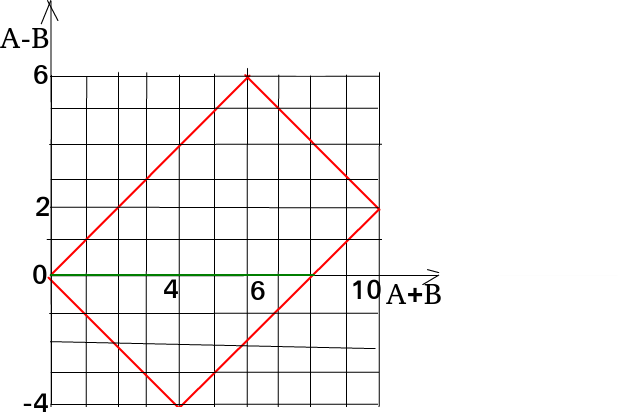
\includegraphics[width=.4\textwidth]{./pictures/t1v2_3.png}
  \caption{Пути}
  \label{fig:23}
\end{figure}

Красным обозначены граничные пути, зелёным --- линия, которой нельзя касаться.
В начале выборов разница у каждого кандидата было 0 голосов, в конце у кандидата $A$ было 6 голосов, а у кандидата $B$ --- 4 голоса.
Поэтому разность голосов в конце составляет 2 голоса.
Перевернём изображение (рис. \ref{fig:231}).

\begin{figure}[h!]
  \centering
  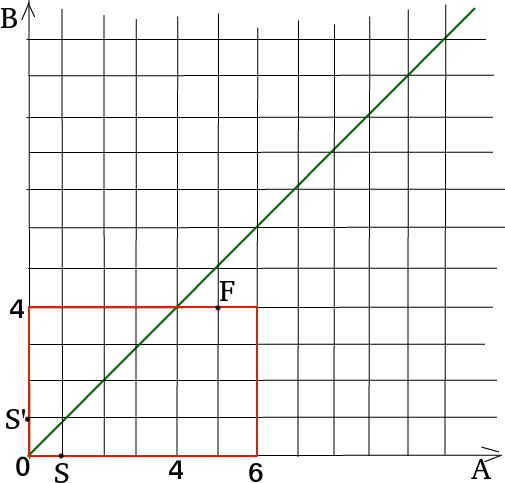
\includegraphics[width=.4\textwidth]{./pictures/t1v2_31.png}
  \caption{Метод отражений}
  \label{fig:231}
\end{figure}

Всего возможных путей есть столько, сколько путей из точки $S$ в точку $F$.
Их
$$ \left| \Omega \right| =
C_{6+4}^4 =
C_{10}^4 =
\frac{10!}{4! \cdot 6!} =
210.$$

Путей из точки $S$ в точку $F$ существует
$$ \left| S \rightarrow F \right| =
C_{5+4}^4 =
C_9^4 =
\frac{9!}{4! \cdot 5!} =
\frac{6 \cdot 7 \cdot 8 \cdot 9}{2 \cdot 3 \cdot 4} =
\frac{6 \cdot 7 \cdot 9}{2} =
2 \cdot 7 \cdot 9 =
149.$$
Путей, которые касаются диагонали ---
$$ \left| S' \rightarrow F \right| =
C_{5+3}^3 =
C_8^3 =
\frac{8!}{3! \cdot 5!} =
\frac{6 \cdot 7 \cdot 8}{2 \cdot 3} =
7 \cdot 8 =
56.$$

Тогда путей,
которые не пересекают диагональ и удовлетворяют указанному в условии событию $C$ будет
$ \left| C \right| =
\left| S \rightarrow F \right| - \left| S' \rightarrow F \right| =
189 - 56 =
133$.
И его вероятность равна
$$P \left( C \right) =
\frac{ \left| C \right| }{ \left| \Omega \right| } =
\frac{183}{210}.$$

\subsubsection*{4}

\textit{Задание.} На отрезок наугад брошено две точки.
Найдите вероятность того, что из трёх образованных отрезков можно составить треугольник.

\textit{Решение.} Пусть отрезок начинается в точке 0 и заканчивается в точке $c$.
Выбираем на нём наугад две точки: точку $a$ и точку $b$, причём $a$ лежит не правее $b$ (рис. \ref{fig:24}).

\begin{figure}[h!]
  \centering
  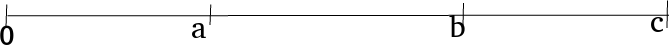
\includegraphics[width=.4\textwidth]{./pictures/t1v2_4.png}
  \caption{Отрезок $ \left[ 0, c \right] $}
  \label{fig:24}
\end{figure}

Тогда пространство элементарных исходов имеет вид $ \Omega =  \\
= \left\{ \left( a, b \right): 0 \leq a \leq b \leq c \right\} $.
Изобразив его на плоскости, видим, что это прямоугольный треугольник с катетами длиной $c$ (рис. \ref{fig:241}).

\begin{figure}[h!]
  \centering
  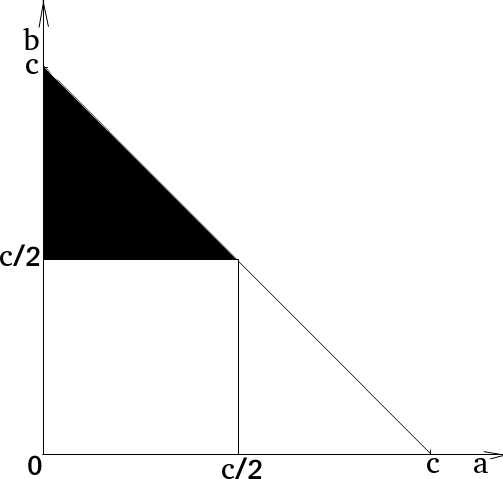
\includegraphics[width=.4\textwidth]{./pictures/t1v2_41.png}
  \caption{Пространство элементарных событий $ \Omega$ и событие $A$}
  \label{fig:241}
\end{figure}

Площадь треугольника равна
$$S_{ \Omega } =
\frac{1}{2} \cdot c \cdot c =
\frac{c^2}{2}.$$

Событие
$$A = \left\{ \left( a, b \right) \in \Omega: a \leq \frac{c}{2}, b \geq \frac{c}{2}, a \leq \frac{c}{2} + b \right\}.$$
Точки множества $A$ образуют прямоугольный треугольник с катетами $c/2$.
Его площадь равна
$$S_A =
\frac{1}{2} \cdot \frac{c}{2} \cdot \frac{c}{2} =
\frac{c^2}{8}.$$

Тогда вероятность события $A$ равна
$$P \left( A \right) =
\frac{S_A}{S_{ \Omega }} =
\frac{c^2}{8} \cdot \frac{2}{c^2} =
\frac{1}{4}.$$

\subsubsection*{5}

\textit{Задание.} В первой урне находятся 3 чёрных и 3 белых шарика, а во второй --- 2 чёрных и 3 белых шарика.
Из второй урны наугад вынули два шарика и переложили в первую.
После этого из первой урны вынимают два шарика.
Найдите вероятность того, что они окажутся разного цвета.

\textit{Решение.} Введём событие $A =$ \{вынутые после перекладывания шарики из первой урны окажутся разного цвета\}.
Введём гипотезы по поводу того,
каких цветов оказались шарики,
переложенные в первую урну из второй: $H_1 =$ \{чёрный, белый\}, $H_2 =$ \{белый, чёрный\}, $H_3 =$ \{чёрный, чёрный\}, $H_4 =$ \{белый, белый\}.
Найдём вероятности этих гипотез:
$$P \left( H_1 \right) =
\frac{2}{5} \cdot \frac{3}{4}, \,
P \left( H_2 \right) =
\frac{3}{5} \cdot \frac{2}{4}, \,
P \left( H_3 \right) =
\frac{2}{5}, \,
P \left( H_4 \right) =
\frac{3}{5}.$$

Найдём условные вероятности события $A$ при условии выполнения каждой из этих гипотез.
Пусть произошла гипотеза $H_1$.
Тогда в первой урне стало 4 чёрных и 4 белых шарика.
Вероятность того, что 2 вынутые шарика окажутся разного цвета, равна
$$P \left( \left. A \right| H_1 \right) =
\frac{4}{8} \cdot \frac{4}{7} \cdot 2.$$
Пусть произошла гипотеза $H_2$.
Тогда в первой урне стало 4 чёрных и 4 белых шарика.
Вероятность того, что 2 вынутые шарика окажутся разного цвета, равна
$$P \left( \left. A \right| H_2 \right) =
\frac{4}{8} \cdot \frac{4}{7} \cdot 2.$$
Пусть произошла гипотеза $H_3$.
Тогда в первой урне стало 5 чёрных и 3 белых шарика.
Вероятность того, что 2 вынутые шарика окажутся разного цвета, равна
$$P \left( \left. A \right| H_3 \right) =
\frac{5}{8} \cdot \frac{3}{7} \cdot 2.$$
Пусть произошла гипотеза $H_4$.
Тогда в первой урне стало 3 чёрных и 5 белых шарика.
Вероятность того, что 2 вынутые шарика окажутся разного цвета, равна
$$P \left( \left. A \right| H_4 \right) =
\frac{3}{8} \cdot \frac{5}{7} \cdot 2.$$

По формуле для полной вероятности
\begin{equation*}
\begin{split}
P \left( A \right) =
\sum \limits_{i=1}^4 P \left( H_i \right) \cdot P \left( \left. A \right| H_i \right).
\end{split}
\end{equation*}

\addcontentsline{toc}{section}{Вариант 3}
\section*{Вариант 3}

\subsubsection*{1}

\textit{Задание.} Что вероятней: выиграть у равносильного противника 3 шахматных партии из 4 или 5 партий из 8?

\textit{Решение.} Найдём вероятность выиграть 3 шахматные партии из четырёх.
Пространство элементарных событий состоит из $ \left| \Omega_1 \right| = 2^4$ элементов,
так как каждую из четырёх партий можно выиграть или проиграть.
Введём событие $A =$ \{3 партии из четырёх будут удачными\}.
Нужно выбрать одну партию из четырёх, которая не будет удачной --- это $C_4^1 = \left| A \right| $.
Тогда вероятность этого события равна
$$P \left( A \right) =
\frac{ \left| A \right| }{ \left| \Omega_1 \right| } =
\frac{C_4^1}{2^4} =
\frac{4}{4^2} =
\frac{1}{4}.$$

Найдём вероятность выиграть 4 шахматные партии из восьми.
Пространство элементарных событий в данном случае состоит из $ \left| \Omega_2 \right| = 2^8$ элементов.
Пусть событие $B =$ \{5 партий из восьми закончатся победой\}.
Нужно выбрать 5 партий из восьми, которые закончатся победой --- это
$$ \left| B \right| =
C_8^5 =
\frac{8!}{5! \cdot 3!} =
\frac{6 \cdot 7 \cdot 8}{2 \cdot 3} =
7 \cdot 8.$$
Тогда вероятность этого события равна
$$P \left( B \right) =
\frac{ \left| B \right| }{ \left| \Omega \right| } =
\frac{7  \cdot 8}{2^8} =
\frac{7}{2^5} =
\frac{7}{32}.$$

Сравним две полученные вероятности.
Для этого первую умножим на 8:
$$ \frac{8}{8} \cdot \frac{1}{4} =
\frac{8}{32}.$$
Видим, что
$$ \frac{8}{32} > \frac{7}{32},$$
поэтому $P \left( A \right) > P \left( B \right) $.
Тогда вероятность выиграть 3 шахматные партии из четырёх больше, чем вероятность выиграть 5 партий из восьми.

\subsubsection*{2}

\textit{Задание.} В сундуке лежат 9 красных, 6 синих и 5 зелёных пуговиц.
Наугад вынули 2 пуговицы.
Найдите вероятность того, что пуговицы разного цвета, если известно, что среди них нет зелёных.

\textit{Решение.} Опишем событие $A =$ \{среди двух пуговиц нет зелёных\}.
Возможны варианты: (красная, красная), (синяя, синяя), (красная, синяя), (синяя, красная).
Вероятность того, что вытянем одну красную и одну синюю пуговицу, равна
$$ \frac{9}{20} \cdot \frac{6}{19}.$$
Вероятность того, что две пуговицы будут красными, равна
$$ \frac{9}{20} \cdot \frac{8}{19}.$$
Наконец, вероятность того, что две пуговицы будут синими, равна
$$ \frac{6}{20} \cdot \frac{5}{19}.$$
Тогда по правилу суммы имеем вероятность указанного события:
\begin{equation*}
\begin{split}
P \left( A \right) =
\frac{2 \cdot 9 \cdot 6}{20 \cdot 19} + \frac{9 \cdot 8}{20 \cdot 19} + \frac{6 \cdot 5}{20 \cdot 19} =
\frac{9 \cdot 6 + 9 \cdot 4 + 3 \cdot 5}{10 \cdot 19} =
\frac{54 + 36 + 15}{10 \cdot 19} = \\
= \frac{105}{10 \cdot 19} =
\frac{21}{2 \cdot 19}.
\end{split}
\end{equation*}

Введём событие $B =$ \{пуговицы оказались разного цвета\}.
Найдём пересечение двух событий: $A \cap B =$ \{пуговицы оказались разного цвета, и среди них нет зелёных\}.
Есть два варианта: (красный, синий), (синий, красный).
Вероятность этого пересечения равна
$$P \left( A \cap B \right) =
\frac{2 \cdot 9 \cdot 6}{20 \cdot 19} =
\frac{9 \cdot 6}{10 \cdot 19} =
\frac{9 \cdot 3}{5 \cdot 19}.$$

Тогда по формуле для условной вероятность получаем, что
$$P \left( \left. B \right| A \right) =
\frac{P \left( A \cap B \right) }{P \left( A \right) } =
\frac{9 \cdot 3}{5 \cdot 19} \cdot \frac{2 \cdot 19}{21} =
\frac{9 \cdot 2}{5 \cdot 7} =
\frac{18}{35}.$$

\subsubsection*{3}

\textit{Задание.} На отрезок наугад брошены две точки.
Найдите вероятность того, что левый из трёх образованных отрезков будет самым коротким.

\textit{Решение.} Пусть отрезок начинается в точке 0 и заканчивается в точке $c$.
Выбираем на нём наугад две точки: точку $a$ и точку $b$, причём $a$ лежит не правее $b$ (рис. \ref{fig:24}).

Тогда пространство элементарных исходов имеет вид $ \Omega =  \\
= \left\{ \left( a, b \right): 0 \leq a \leq b \leq c \right\} $.
Изобразив его на плоскости, видим, что это прямоугольный треугольник с катетами длиной $c$ (рис. \ref{fig:33}).

\begin{figure}[h!]
  \centering
  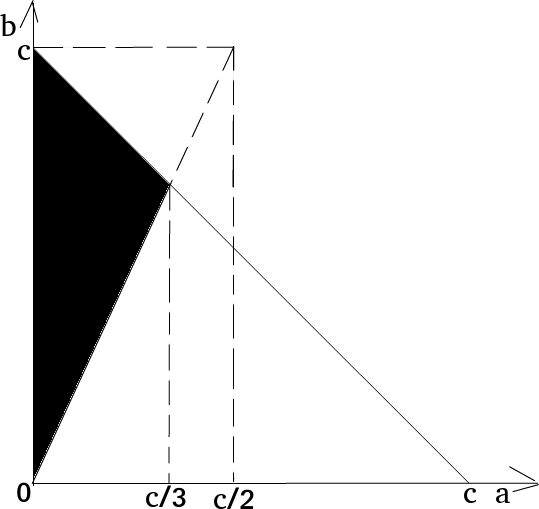
\includegraphics[width=.4\textwidth]{./pictures/t1v3_3.png}
  \caption{Пространство элементарных событий $ \Omega$ и событие $A$}
  \label{fig:33}
\end{figure}

Площадь треугольника равна
$$S_{ \Omega } =
\frac{1}{2} \cdot c \cdot c =
\frac{c^2}{2}.$$

Пусть событие $A = \left\{ \left( a, b \right) \in \Omega: a \leq b-a, a \leq c-b \right\} $.
Изобразив его на рисунке, видим, что это треугольник, образованный прямой $b = c - a$, прямой $b = 2a$ и одним из катетов исходного треугольника.
Его площадь найдём с помощью интеграла:
$$S_1 =
\int \limits_0^{ \frac{c}{3} } \left( c - a \right) da =
\left. \left( ca - \frac{a^2}{2} \right) \right|_0^{ \frac{c}{3} } =
c \cdot \frac{c}{3} - \frac{c^2}{9 \cdot 2} =
\frac{c^2}{3} - \frac{c^2}{18} =
\frac{6c^2 - c^2}{18} =
\frac{5c^2}{18}.$$
От этой площади нужно отнять площадь треугольника под прямой $b = 2a$.
Она равна
$$S_2 =
\frac{1}{2} \cdot \frac{c}{3} \cdot \frac{2c}{3} =
\frac{c^2}{9}.$$

Площадь треугольника равна
$$S_A =
S_1 - S_2 =
\frac{c^2}{6}.$$

Тогда вероятность этого события равна
$$P \left( A \right) =
\frac{S_A}{S_{ \Omega }} =
\frac{1}{3}.$$

\subsubsection*{4}

\textit{Задание.} Частица совершает случайное симметрическое блуждание на прямой, делая шаг вправо или влево с вероятностью $1/2$.
Найдите вероятность того, что через $2n$ шагов частица впервые вернётся в исходную точку.

\textit{Решение.} Задача изображена на рисунке \ref{fig:34}.

\begin{figure}[h!]
  \centering
  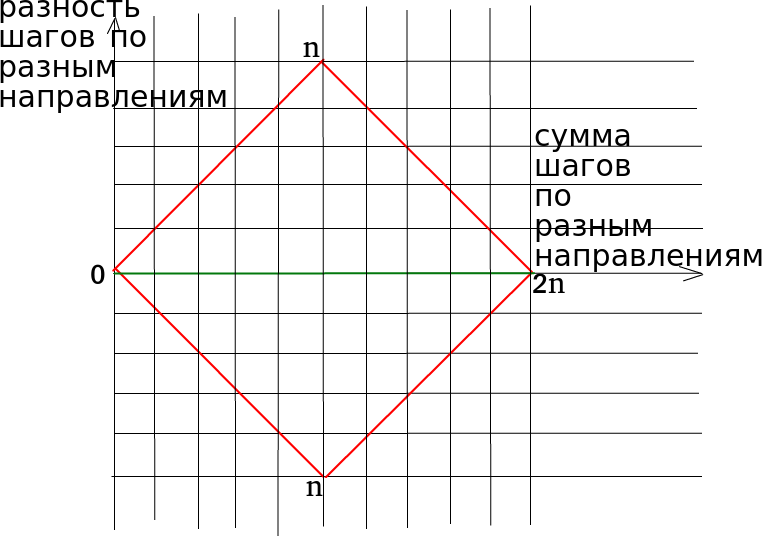
\includegraphics[width=.4\textwidth]{./pictures/t1v3_4.png}
  \caption{Задача про случайное блуждание частицы на прямой}
  \label{fig:34}
\end{figure}

Красным обозначены крайние пути, зелёным --- линия, которую нельзя пересекать.
Перевернём изображение (рис. \ref{fig:341}).

\begin{figure}[h!]
  \centering
  \includegraphics[width=.4\textwidth]{./pictures/t1v3_41.png}
  \caption{Метод отражений}
  \label{fig:341}
\end{figure}

Всего путей
$$ \left| \Omega \right| =
2^{2n}.$$

Начальная точка --- точка $A$, конечная --- точка $B$.
Всего путей из $A$ в $B$ существует
$$ \left| A \rightarrow B \right| =
C_{n+n}^n =
C_{2n}^n =
\frac{ \left( 2n \right)!}{n!n!}.$$

Путей, которые пересекают диагональ будет
$$ \left| A \rightarrow B' \right| =
C_{n+n-1}^n =
C_{2n-1}^n =
\frac{ \left( 2n-1 \right)!}{n! \left( n-1 \right)!}.$$

Тогда путей, которые не пересекают диагональ будет
\begin{equation*}
\begin{split}
2 \left( \left| A \rightarrow B \right| - \left| A \rightarrow B' \right| \right) =
2 \cdot \left( \frac{ \left( 2n \right)!}{n!n!} - \frac{ \left( 2n-1 \right)!}{n! \left( n-1 \right)!} \right) = \\
= 2 \left( \frac{ \left( 2n \right)!}{n! \left( n-1 \right)!n} - \frac{ \left( 2n-1 \right)!}{n! \left( n-1 \right)!} \right) =
2 \cdot \frac{ \left( 2n \right)! - \left( 2n-1 \right)!n}{n!n!} = \\
= 2 \cdot \frac{ \left( 2n-1 \right)! \left( 2n-n \right)}{n!n!} =
\frac{2 \left( 2n-1 \right)!n}{n!n!} =
\frac{2 \left( 2n-1 \right)!}{n! \left( n-1 \right)!},
\end{split}
\end{equation*}
так как частица может двигаться и вправо, и влево.

Тогда вероятность указанного в условии задачи события равна
$$P =
\frac{2 \left( 2n-1 \right)!}{n! \left( n-1 \right)! \cdot 2^{2n}} =
\frac{\left( 2n-1 \right)!}{n! \left( n-1 \right)! \cdot 2^{2n-1}}.$$

\subsubsection*{5}

\textit{Задание.}
Среди 5 стрелков есть 3 хороших, которые метко стреляют с вероятностью $0.8$, и 2 средних, которые попадают в цель с вероятностью $0.5$.
Вызвали наугад двух стрелков, они выстрелили по мишени и оба попали.
Найдите вероятность того, что стреляли два средних стрелка.

\textit{Решение.}
Введём событие $A =$ \{два стрелка попали по мишени\} и гипотезы о том,
каких стрелков вызвали: $H_1 =$ \{оба стрелка были хорошими\},
$H_2 =$ \{оба стрелка были средними\}, $H_3 =$ \{первый стрелок был хорошим, а второй --- средним\}, $H_4 =$ \{первый стрелок был средним, а второй хорошим\}.
Нужно найти вероятность
$$P \left( \left. H_2 \right| A \right) =
\frac{P \left( \left. A \right| H_2 \right) P \left( H_2 \right) }{ \sum \limits_{i=1}^4 P \left( \left. A \right| H_i \right) P \left( H_i \right) }.$$

Вероятность того, что выбрали два хороших стрелка равна
$$P \left( H_1 \right) =
\frac{3}{5} \cdot \frac{2}{4} =
\frac{3}{5} \cdot \frac{1}{2} =
\frac{3}{10}.$$

Вероятность того, что выбрали два средних стрелка равна
$$P \left( H_2 \right) =
\frac{2}{5} \cdot \frac{1}{4} =
\frac{1}{5 \cdot 2} =
\frac{1}{10}.$$

Вероятность того, что один из стрелков был хорошим, а второй --- средним равна
$$P \left( H_3 \right) =
P \left( H_4 \right) =
\frac{3}{5} \cdot \frac{2}{4} =
\frac{3}{10}.$$

Найдём условные вероятности:
\begin{equation*}
\begin{split}
P \left( \left. A \right| H_1 \right) =
\frac{8}{10} \cdot \frac{8}{10} =
\frac{4}{5} \cdot \frac{4}{5} =
\frac{16}{25}, \,
P \left( \left. A \right| H_2 \right) =
\frac{1}{2} \cdot \frac{1}{2} =
\frac{1}{4}, \,
P \left( \left. A \right| H_3 \right) = \\
= P \left( \left. A \right| H_4 \right) =
\frac{8}{10} \cdot \frac{1}{2} =
\frac{4}{5 \cdot 2} =
\frac{2}{5}.
\end{split}
\end{equation*}

Тогда по формуле Байеса получаем
$$P \left( \left. H_2 \right| A \right) =
\frac{ \frac{1}{4} \cdot \frac{1}{10} }{ \frac{3}{10} \cdot \frac{16}{25} + \frac{1}{4} \cdot \frac{1}{10} + 2 \cdot \frac{3}{10} \cdot \frac{2}{5} }$$

\addcontentsline{toc}{chapter}{Занятие 7. Алгебры и $ \sigma $-алгебры. Мера}
\chapter*{Занятие 7. Алгебры и $ \sigma $-алгебры. Мера}

\addcontentsline{toc}{section}{Контрольные вопросы и задания}
\section*{Контрольные вопросы и задания}

\subsubsection*{Приведите определение алгебры событий,
$ \sigma $-алгебры событий, конечно-аддитивной меры, счётно-аддитивной меры, вероятностной меры, монотонного класса.}

Совокупность $\mathcal{A}$ подмножеств называется алгеброй, если выполнены свойства:
\begin{enumerate}
\item $ \emptyset \in \mathcal{A}$,
\item $A \in \mathcal{A} \Rightarrow \overline{A} \in \mathcal{A}$,
\item $A, B \in \mathcal{A} \Rightarrow A \cup B \in \mathcal{A}$.
\end{enumerate}

Совокупность множеств называется $ \sigma $-алгеброй, если выполняются следующие условия:
\begin{enumerate}
\item $ \Omega \in \mathcal{A}$,
\item $A \in \mathcal{A} \Rightarrow \overline{A} \in \mathcal{A}$,
\item $A_1, \dotsc, A_n \in \mathcal{A} \Rightarrow \bigcup \limits_{i=1}^n A_i \in \mathcal{A}$.
\end{enumerate}

Функция $ \mu: \mathcal{F} \rightarrow \left[ 0, \infty \right] $ называется конечно-аддитивной мерой (иногда объёмом), если она удовлетворяет следующим аксиомам:
\begin{enumerate}
\item $ \mu \left( \emptyset \right) = 0$,
\item если
$ \left\{ E_n \right\}_{n=1}^N \subset \mathcal{F}$
--- конечное семейство попарно непересекающихся множеств из
$ \mathcal{F}$, то есть $E_i \cap E_j = \emptyset, \, i \neq j$,
то $ \mu \left( \bigcup \limits_{n=1}^N E_n \right) = \sum \limits_{n=1}^N \mu \left( E_n \right)$.
\end{enumerate}

Функция $ \mu: \mathcal{F} \rightarrow \left[ 0, \infty \right] $ называется счётно-аддитивной (или $ \sigma $-аддитивной) мерой, если она удовлетворяет следующим аксиомам:
\begin{enumerate}
\item $ \mu \left( \emptyset \right) = 0$,
\item ($ \sigma $-аддитивность) Если
$ \left\{ E_n \right\}_{n=1}^{ \infty } \subset \mathcal{F}$
--- конечное семейство попарно непересекающихся множеств из
$ \mathcal{F}$, то есть $E_i \cap E_j = \emptyset, \, i \neq j$,
то $ \mu \left( \bigcup \limits_{n=1}^{ \infty } E_n \right) = \sum \limits_{n=1}^{ \infty } \mu \left( E_n \right)$.
\end{enumerate}

Вероятностная мера (вероятность) --- это функция $P: \, \mathcal{F} \rightarrow \left[ 0, 1 \right], \mathcal{F} - \sigma $-алгебра:
\begin{enumerate}
\item $P \left( \Omega \right) = 1$,
\item если
$A_n \in \mathcal{F}, \,
A_n \cap A_m = \emptyset, \,
n \neq m$, то $P \left( \bigcup \limits_{n=1}^{ \infty } A_n \right) = \sum \limits_{n=1}^{ \infty  P \left( A_n \right) }$.
\end{enumerate}

Совокупность $ \mu $ подмножеств множества $ \Omega $ называется монотонным классом,
если для любой монотонной последовательности $ \left\{ A_n \right\}_{n=1}^{ \infty } $
(т.е. такой,
что $A_1 \supset A_2 \supset A_3 \supset \dotsc $ или $A_1 \subset A_2 \subset \dotsc $) её предел $ \lim \limits_{n \rightarrow \infty } A_n$ тоже лежит в $ \mu $.

\subsubsection*{Сформулируйте теорему про монотонный класс.}

Пусть $ \mathcal{A}$ --- алгебра подмножеств множества $ \Omega $.
Тогда монотонный класс, порождаемый $ \mathcal{A}$ совпадает с алгеброй, порождаемой $ \mathcal{A}: \, m \left( \mathcal{A} \right) = \sigma \left( \mathcal{A} \right) $.

\addcontentsline{toc}{section}{Аудиторные задачи}
\section*{Аудиторные задачи}

\subsubsection*{7.3}

\textit{Задание.} Опишите $ \sigma $-алгебру подмножеств отрезка $ \left[ 0, 1 \right] $, порождённую множествами:
\begin{enumerate}[label=\alph*)]
\item $ \left[ 0, 1/2 \right] $;
\item $ \left[ 0, 2/3 \right] $ и $ \left[ 1/3, 1 \right] $;
\item $ \left[ 0, 1/2 \right] $ и $ \left[ 1/2,  1 \right] $.
\end{enumerate}

\textit{Решение.} Множество $ \Omega = \left[ 0, 1 \right] $.

\begin{enumerate}[label=\alph*)]
\item $A = \left[ 0, 1/2 \right] $.
Опишем $ \sigma $-алгебру подмножеств:
$$ \mathcal{A}_A =
\left\{ \emptyset, \Omega, A, \overline{A} \right\} =
\left\{ \emptyset, \left[ 0, 1 \right], \left[ 0, \frac{1}{2} \right], \left( \frac{1}{2}, 1 \right] \right\};$$
\item $B = \left[ 0, 2/3 \right], \, C = \left[ 1/3, 1 \right] $.
Введём непересекающиеся множества, которые в объединении дают всё множество:
$$D_1 =
\left[ 0, \frac{1}{3} \right], \,
D_2 =
\left( \frac{1}{3}, \frac{1}{2} \right],
D_3 =
\left( \frac{2}{3}, 1 \right].$$
Тогда
$$ \mathcal{A}_D =
\left\{ \emptyset, \Omega, \bigcup \limits_{i=1}^k D_i, k = \overline{1,3} \right\};$$
\item $A = \left[ 0, 1/2 \right], \, B = \left[ 1/2,  1 \right] $.
Введём непересекающиеся множества, которые в объединении дают всё множество:
$$D_1 =
\left[ 0, \frac{1}{2} \right), \,
D_2 \left\{ \frac{1}{2} \right\}, \,
D_3 = \left( \frac{1}{2}, 1 \right].$$
Тогда
$$ \mathcal{A}_D =
\left\{ \emptyset, \Omega, \bigcup \limits_{i=1}^k D_i, k = \overline{1,3} \right\}.$$
\end{enumerate}

\subsubsection*{7.4}

\textit{Задание.} Пусть $ \mathcal{B} - \sigma $-алгебра, порождённая интервалами $ \left( a, b \right] $.
Докажите, что множества $ \left( a, b \right), \left[ a, b \right], \left\{ a \right\} $ тоже принадлежат $ \mathcal{B} $.

\textit{Решение.} $ \mathcal{B} $ замкнутая относительно конечного объединения или пересечения множеств, которые в неё входят.
$ \mathcal{B} - \sigma $-алгебра.
Рассмотрим интервалы
$$ \left( a, b - \frac{1}{n} \right].$$
Возьмём бесконечное пересечение
$$ \bigcup \limits_{n=1}^{ \infty } \left( a, b - \frac{1}{n} \right].$$
Тогда приблизимся к точке $b$, но сама она входить не будет:
$$ \left( a, b \right) =
\bigcup \limits_{n=1}^{ \infty } \left( a, b - \frac{1}{n} \right].$$
Для любого $n$ отрезок
$$ \left( a, b - \frac{1}{n} \right] $$
по условию принадлежит $ \sigma $-алгебре $ \mathcal{B}$.
Тогда его счётное объединение тоже принадлежит $ \sigma $-алгебре:
$$ \bigcup \limits_{n=1}^{ \infty } \left( a, b - \frac{1}{n} \right] \in \mathcal{B} $$
по определению.
Тогда $ \left( a, b \right) \in \mathcal{B} $.

Отрезок, где оба конца входят,
$$ \left[ a, b \right] =
\bigcap \limits_{n=1}^{ \infty } \left( a - \frac{1}{n}, b \right].$$
В каждый этот интервал точка $a$ входит.
Тогда в их пересечение точка $a$ входит:
$$ \forall n \,
\left( a - \frac{1}{n}, b \right] \in \mathcal{B} \Rightarrow
\bigcap \limits_{n=1}^{ \infty } \left( a - \frac{1}{n}, b \right] \in \mathcal{B} \Rightarrow
\left[ a, b \right] \in \mathcal{B}.$$
Множество, состоящее из одной точки:
$$ \left\{ a \right\} =
\left[ a, a \right] =
\left( a - \frac{1}{n}, a \right].$$
Для любого $n$ отрезок такого вида принадлежит $ \mathcal{B} $, тогда их счётное пересечение принадлежит $ \mathcal{B} $, тогда $ \left[ a, a \right] \in \mathcal{B} $.
А это значит, что $ \left\{ a \right\} \in \mathcal{B} $.

\subsubsection*{7.5}

\textit{Задание.} Пусть $ \Omega = \mathbb{R}^2, \, \mathcal{B} $ --- борелевская $ \sigma $-алгебра в $ \mathbb{R}^2$.
Докажите, что:
\begin{enumerate}[label=\alph*)]
\item $ \left\{ x \in \mathbb{R}^2: \left| \left| x \right| \right| < 1 \right\} \in \mathcal{B} $;
\item $ \left\{ x \in \mathbb{R}^2: \left| \left| x \right| \right| \leq 1 \right\} \in \mathcal{B} $;
\item $ \left\{ \left( 1, 1 \right) \right\} \in \mathcal{B} $;
\item $ \mathbb{Q} \times \mathbb{Q} \in \mathcal{B} $;
\item $ \left[ 0, 1 \right]^2 \in \mathcal{B} $;
\item $ \left( 0, 1 \right) \times \left[ 2, 3 \right) \in \mathcal{B} $;
\item $ \left\{ \left( x_1, x_2 \right) \in \mathbb{R}^2: sin x_1 + cos \left( x_1 + x_2^3 \right) > 1/7 \right\} \in \mathcal{B} $.
\end{enumerate}

\textit{Решение.} Есть борелевская $ \sigma $-алгебра в $ \mathbb{R}^2$.

\begin{enumerate}[label=\alph*)]
\item $ \left\{ x \in \mathbb{R}^2: \left| \left| x \right| \right| < 1 \right\} \in \mathcal{B} $ ---
внутренняя часть круга с центром в точке 0 и радиусом 1, открытое множество, а значит принадлежит $ \sigma $-алгебре, как открытое множество;
\item это замкнутое множество.
И как дополнение к открытому множеству принадлежит $ \sigma $-алгебре;
\item $ \left\{ \left( 1, 1 \right) \right\} $ --- замкнутое множество.
Поэтому принадлежит $ \sigma $-алгебре.
Или $ \left( 1, 1 \right) = \left\{ 1 \right\} \times \left\{ 1 \right\} \in \mathcal{B} \left( \mathbb{R}^2 \right) $;
\item $ \mathbb{Q} $ --- множество рациональных чисел --- счётное множество.
Всякие счётные объединения и пересечения не выводят за границы $ \sigma $-алгебры.
$ \left( r_i, r_j \right) \in \mathcal{B} $ как замкнутое множество (точка).
$ \forall i, j \, \bigcup \limits_{i=1}^{ \infty } \bigcup \limits_{j=1}^{ \infty } \left( r_i, r_j \right) \in \mathcal{B} $.
\item $ \left[ 0, 1 \right]^2$ --- замкнутое множество в $ \mathbb{R}^2 \Rightarrow \left[ 0, 1 \right]^2 \in \\
\in \mathcal{B} \left( \mathbb{R}^2 \right) $.
Второй способ: $ \left[ 0, 1 \right]^2 = \left[ 0, 1 \right] \times \left[ 0, 1 \right] $.
Знаем, что $ \left[ 0, 1 \right] \in \mathcal{B} \left( \mathbb{R} \right) $.
Тогда
$ \left[ 0, 1 \right] \times \left[ 0, 1 \right] \in \mathcal{B} \left( \mathbb{R}^2 \right) \Rightarrow
\left[ 0, 1 \right]^2 \in \mathcal{B} \left( \mathbb{R}^2 \right) $;
\item покажем, что $ \left[ 2, 3 \right) \in \mathcal{B} \left( \mathbb{R} \right) $.
Будем считать, что $ \sigma $-алгебра порождается интервалами $ \left( a, b \right) \in \mathcal{B} \left( \mathbb{R} \right) $.
Можем записать данный интервал в виде
$$ \left( 2, 3 \right) =
\bigcap \limits_{n=1}^{ \infty } \left( 2 - \frac{1}{n}, 3 \right).$$
В каждый этот интервал точка 2 входит.
Тогда точка 2 входит в пересечение, потому что отступили влево.
Тогда $ \left[ 2, 3 \right) \in \mathcal{B} \left( \mathbb{R} \right) $.
По определению $ \left( 0, 1 \right) \in \mathcal{B} \left( \mathbb{R} \right) $ (это открытое множество).
Тогда $ \left( 0, 1 \right) \times \left[ 2, 3 \right) \in \mathcal{B} $;
\item функции $sin x_1 $ и $cos \left( x_1 + x_2^3 \right) $ ---
ограниченные: $-1 \leq sin x_1 \leq 1, \, -1 \leq \\
\leq cos \left( x_1 + x_2^3 \right) \leq 1$.
А интервалы по определению $ \mathcal{B} \left( \mathbb{R} \right) $ ей принадлежат.
Тогда $ \left\{ \left( x_1, x_2 \right) \in \mathbb{R}^2: sin x_1 + cos \left( x_1 + x_2^3 \right) > 1/7 \right\} \in \mathcal{B} $.
\end{enumerate}

\subsubsection*{7.6}

\textit{Задание.} Пусть $ \mu $ --- конечно-аддитивная мера на алгебре $ \mathcal{B} $ и пусть множества $A, A_1, A_2, \dotsc $ принадлежат $ \mathcal{B} $.
Докажите, что если:
\begin{enumerate}[label=\alph*)]
\item $A = \bigcup \limits_{n=1}^k A_n$ и $A_n$ попарно не пересекаются, то $ \mu \left( A \right) = \sum \limits_{n=1}^k \mu \left( A_n \right) $;
\item $A = \bigcup \limits_{n=1}^{ \infty } A_n$ и $A_n$ попарно не пересекаются, то $ \mu \left( A \right) \geq \sum \limits_{n=1}^{ \infty } \mu \left( A_n \right) $.
\end{enumerate}

\textit{Решение.}
\begin{enumerate}[label=\alph*)]
\item $A = \bigcup \limits_{n=1}^k A_n, \, A_i \cap A_j = \emptyset, \, i \neq j$.
Тогда $ \mu \left( A \right) = \sum \limits_{n=1}^k \mu \left( A_n \right) $ --- следует из определения конечно-аддитивной меры;
\item $A = \bigcup \limits_{n=1}^{ \infty } A_n, \, A_i \cap A_j = \emptyset, \, i \neq j$.
Каждое конечное объединение принадлежит множеству $A$.
Для произвольного $k \geq 1$ рассмотрим конечное объединение: $ \bigcup \limits_{n=1}^k A_n \subset \bigcup \limits_{n=1}^{ \infty } A_n = A$.
Из монотонности можем утверждать, что $ \mu \left( \bigcup \limits_{n=1}^k A_n \right) \leq \mu \left( A \right) $.
Мера конечно-аддитивна, и множества не пересекаются.
Из определения конечно-аддитивной меры
$ \mu \left( \bigcup \limits_{n=1}^k A_n \right) \leq
\sum \limits_{n=1}^k \mu \left( A_n \right) \leq
\mu \left( A \right) \,
\forall k$.
Переходя к границе при $ k \rightarrow \infty $ получаем $ \sum \limits_{n=1}^{ \infty } \mu \left( A_n \right) \leq \mu \left( A \right) $ ---
для $A_i \cap A_j = \emptyset, \, i \neq j$.
\end{enumerate}

\subsubsection*{7.7}

\textit{Задание.} Пусть $ \mu $ --- неотрицательная аддитивная функция, которая задана на алгебре $ \mathcal{B} $.
Докажите, что $ \mu $ является $ \sigma $-аддитивной функцией тогда и только тогда,
когда для произвольных множеств $A, A_1, A_2, \dotsc $,
которые принадлежат $ \mathcal{B} $, из того,
что $A \subset \bigcup \limits_{n=1}^{ \infty } A_n$ следует, что $ \mu \left( A \right) \leq \sum \limits_{n=1}^{ \infty } \mu \left( A_n \right) $.

\textit{Решение.}$ \mu $ --- некоторая неотрицательная аддитивная функция на алгебре $ \mathcal{B} $.
Доказать, что $ \mu - \sigma $-аддитивная мета тогда и только тогда, если из того,
что $A \subset \bigcup \limits_{n=1}^{ \infty }$ следует, что $ \mu \left( A \right) \leq \sum \limits_{n=1}^{ \infty } \mu \left( A_n \right) $.

Пусть $ \mu - \sigma $-аддитивная.
Это означает,
что имеем $ \mu \left( \bigcup \limits_{n=1}^{ \infty } A_n \right) = \sum \limits_{n=1}^{ \infty } \mu \left( A_n \right) $ для множеств,
которые не пересекаются $ \left( A_i \cap A_j = \emptyset, \, i \neq j \right) $.

Если $A \subset \bigcup \limits_{n=1}^{ \infty } A_n$, то по монотонности $ \mu \left( A \right) \leq \mu \left( \bigcup \limits_{n=1}^{ \infty } A_n \right) $.

Объединение множеств, которые не пересекаются обозначим как $ \bigcup \limits_{n=1}^{ \infty } A_m = \\
= \bigsqcup \limits_{n=1}^{ \infty } B_n$,
где $B_1 = A_1, \, B_2 = A_2 \cap \overline{A_1}, \, B_3 = A_3 \cap \overline{A_2} \cap \overline{A_1}, \dotsc $.

Откуда следует,
что
$ \mu \left( \bigcup \limits_{n=1}^{ \infty } A_n \right) =
\mu \left( \bigsqcup \limits_{n=1}^{ \infty } B_n \right) =
\sum \limits_{n=1}^{ \infty } \mu \left( B_n \right) \leq
\sum \limits_{n=1}^{ \infty } \mu \left( A_n \right) $.

Имеем, что $B_2 = A_2 \cap C \Rightarrow B_2 \subseteq A_2 \Rightarrow \mu \left( B_2 \right) \leq \mu \left( A_2 \right) $.
Поэтому $ \mu \left( A \right) \leq \\
\leq \sum \limits_{n=1}^{ \infty } \mu \left( A_n \right) $.
В одну сторону доказали.
Знаем,
что
$A \subset \bigcup \limits_{n=1}^{ \infty } A_n \Rightarrow
\mu \left( A \right) \leq \\
\leq \mu \left( \bigcup \limits_{n=1}^{ \infty } A_n \right) \leq
\sum \limits_{n=1}^{ \infty } \mu \left( A_n \right) $
выполняется для любых множеств $A, A_1, A_2, \dotsc $.
По предыдущей задаче (задача 7.6) $ \mu \left( A \right) \geq \sum \limits_{n=1}^k \mu \left( A_n \right) $ для множеств, которые не пересекаются.
Для множеств, которые не пересекаются возможно только равенство:
$ \mu \left( A \right) = \sum \limits_{n=1}^{ \infty } \mu \left( A_n \right) $ для $A_i \cap A_j = \emptyset, \, i \neq j$.

\subsubsection*{7.8}

\textit{Задание.} Пусть $ \Omega $ --- множество рациональных точек на $ \left[ 0, 1 \right] $, а $ \mathcal{F} $ ---
алгебра множеств,
каждое из которых является бесконечной суммой множеств $A$ вида
$ \left\{ r: \, a < r < b \right\}, \,
\left\{ r: \, a < r \leq b \right\}, \,
\left\{ r: \, a \leq r < b \right\} $,
которые не пересекаются, и пусть $P \left( A \right) = b - a$.
Докажите, что $P$ является конечно-аддитивной, но не счётно-аддитивной функцией множеств.

\textit{Решение.} $ \Omega = \left\{ \left[ 0, 1 \right] \cap \mathbb{Q} \right\} $ --- множество рациональных точек.
$ \mathcal{F} $ --- алгебра множеств, порождённая интервалами любого вида (открытыми, полуоткрытыми, замкнутыми).
Хотим показать, что $P = b - a$ --- конечно-аддитивная, но не счётно-аддитивная.

$ \mathbb{Q} $ --- счётное множество, $ \mathbb{Q} = \bigcup \limits_{i=1}^{ \infty } \left\{ r_i \right\} $.
Длина отрезка $ \left[ 0, 1 \right] - P \left( \Omega \right) = 1$.
Если бы $P$ была счётно-аддитивной мерой, то должно бы быть,
что
$P \left( \Omega \right) = \\
= P \left( \bigcup \limits_{i=1}^{ \infty } \left\{ r_i \right\} \right) =
\sum \limits_{i=1}^{ \infty } P \left( \left\{ r_i \right\} \right) $.
Каждое $P \left( \left\{ r_i \right\} \right) = 0$, так как $ \left\{ r_i \right\} $ --- замкнутый интервал с концами $r_i, r_i$.
Поэтому $P \left( \Omega \right) = 0$ --- противоречие.
Поэтому $P$ не является счётно-аддитивной мерой.

\subsubsection*{7.9}

\textit{Задание.}
На алгебре всех подмножеств множества рациональных чисел отрезка $ \left[ 0, 1 \right] $ введите меру так,
чтобы мера каждого рационального числа была положительной, а мера множества всех рациональных чисел из $ \left[ 0, 1 \right] $ была бы равна единице.

\textit{Решение.}
$ \Omega = \left\{ \mathbb{Q} \cap \left[ 0, 1 \right] \right\} $ --- счётное множество, счётный набор рациональных точек:
$ \Omega =
\left\{ r_1, r_2, \dotsc, r_n, \dotsc \right\} $.

Хотим,
чтобы
$P \left( \Omega \right) =
1 =
\sum \limits_{n=1}^{ \infty } P \left( \left\{ r_n \right\} \right) =
P \left( \left\{ r_1 \right\} \right) + P \left( \left\{ r_2 \right\} \right) + \dotsc $.

Каждое $P \left( \left\{ r_n \right\} \right) $ больше нуля и меньше единицы.

Просуммируем:
$$\sum \limits_{k=1}^{ \infty } \left( \frac{1}{2} \right)^k =
\frac{ \frac{1}{2} }{1 - \frac{1}{2} } =
1.$$
Поэтому все вероятности не нулевые и в сумме дают единицу.

\subsubsection*{7.10}

\textit{Задание.} Может ли число всех событий некоторого вероятностного пространства равняться 129; 130; 128?

\textit{Решение.} Число всех событий некоторого вероятностного пространства может равняться числу, которое является степенью двойки.
Числа 129 и 130 не являются степенями двойки, поэтому не могут быть числом всех событий некоторого вероятностного пространства.
А число $128 = 2^7$, поэтому может быть числом всех событий некоторого вероятностного пространства.

\addcontentsline{toc}{section}{Домашнее задание}
\section*{Домашнее задание}

\subsubsection*{7.12}

\textit{Задание.} Опишите $ \sigma $-алгебру подмножеств отрезка $ \left[ 0, 1 \right] $, порождённую множествами:
\begin{enumerate}[label=\alph*)]
\item $ \left[ 1/3, 1/2 \right] $;
\item множеством рациональных точек отрезка $ \left[ 0, 1 \right] $;
\item $ \left\{ 0 \right\} $ и $ \left\{ 1 \right\} $.
\end{enumerate}

\textit{Решение.} Множество $ \Omega = \left[ 0, 1 \right] $.

\begin{enumerate}[label=\alph*)]
\item $A = \left[ 1/3, 1/2 \right] $.
Опишем $ \sigma $-алгебру подмножеств:
$$ \mathcal{A}_A =
\left\{ \emptyset, \Omega, A, \overline{A} \right\} =
\left\{ \emptyset, \left[ 0, 1 \right],
\left[ \frac{1}{3}, \frac{1}{2} \right], \left[ 0, \frac{1}{3} \right) \cup \left( \frac{1}{2}, 1 \right] \right\};$$
\item пусть $B = \mathbb{Q} \cap \left[ 0, 1 \right] $ --- множество рациональных точек отрезка $ \left[ 0, 1 \right] $.
Тогда
$ \mathcal{A}_{ \mathbb{Q} } =
\left\{ \emptyset, \Omega, B, \overline{B} \right\} =
\left\{ \emptyset, \left[ 0, 1 \right], \mathbb{Q} \cap \left[ 0, 1 \right], \left[ 0, 1 \right] \setminus \mathbb{Q} \right\};$
\item $C = \left\{ 0 \right\}, E = \left\{ 1 \right\} $.
Введём непересекающиеся множества,
которые в объединении дают весь отрезок: $D_1 = \left\{ 0 \right\}, \, D_2 = \left( 0, 1 \right), \, D_3 = \left\{ 1 \right\} $.
Тогда
$ \mathcal{A}_D =
\left\{ \emptyset, \Omega, \bigcup \limits_{i=1}^k D_i, k = \overline{1, 3} \right\} = \\
= \left\{ \emptyset, \left[0, 1 \right], \left\{ 0 \right\}, \left( 0, 1 \right),
\left\{ 1 \right\}, \left[0, 1 \right), \left(0, 1 \right], \left\{ 0 \right\} \cup \left\{ 1 \right\} \right\} $.
\end{enumerate}

\subsubsection*{7.13}

\textit{Задание.} Пусть $ \Omega = \mathbb{R}, \, \mathcal{B} $ --- борелевская $ \sigma $-алгебра на $ \mathbb{R} $.
Докажите, что $ \mathbb{R} \setminus \mathbb{Q} \in \mathcal{B} $.

\textit{Решение.} Минимальная $ \sigma $-алгебра,
содержащая множество всех интервалов на вещественной прямой,
называется борелевской $ \sigma $-алгеброй в $ \mathbb{R} $ и обозначается $ \mathcal{B} \left( \mathbb{R} \right) $.

Борелевская $ \sigma $-алгебра содержит все закрытые интервалы на $ \mathbb{R} $.
Любое счётное объединение закрытых интервалов на $ \mathbb{R} $ принадлежит $ \mathcal{B} \left( \mathbb{R} \right) $.
Тогда можем взять все рациональные числа $q$ из $ \mathbb{Q} $, которых счётное количество.
Тогда берём множество закрытых интервалов вида $ \left[ q, q \right], q \in \mathbb{Q} $.
Объединение всех этих множеств,
которые принадлежат $ \mathcal{B} \left( \mathbb{R} \right) $ по определению даст множество,
принадлежащее $ \mathcal{B} \left( \mathbb{R} \right) $, т.е. множество $ \mathbb{Q} \in \mathcal{B} \left( \mathbb{R} \right) $.
Тогда его дополнение $ \overline{ \mathbb{Q} } = \mathbb{R} \setminus \mathbb{Q} \in \mathcal{B} \left( \mathbb{R} \right) $.

\subsubsection*{7.14}

\textit{Задание.} Пусть $ \Omega = \mathbb{R}, \, \mathcal{B} $ --- борелевская $ \sigma $-алгебра на $ \mathbb{R}^2$.
Докажите, что:
\begin{enumerate}[label=\alph*)]
\item $ \left( \mathbb{R} \setminus \mathbb{Q} \right) \times \mathbb{Q} \in \mathcal{B} \left( \mathbb{R}^2 \right) $;
\item $ \left\{ \left( x_1, x_2 \right) \in \mathbb{R}^2:
max \left( sin \left( x_1 x_2 \right), arctg \left( x_2 - x_1 \right) \right) > 0.1 \right\} \in \mathcal{B} \left( \mathbb{R}^2 \right) $.
\end{enumerate}

\textit{Решение.}
\begin{enumerate}[label=\alph*)]
\item $ \mathbb{R} \setminus \mathbb{Q} \in \mathcal{B} \left( \mathbb{R} \right), \,
\mathbb{Q} \in \mathcal{B} \left( \mathbb{R} \right) \Rightarrow
\left( \mathbb{R} \setminus \mathbb{Q} \right) \times \mathbb{Q} \in \mathcal{B} \left( \mathbb{R}^2 \right) $;
\item функции $arctg \phi $ и $sin \phi $ --- ограниченные.
В случае максимума синуса функция будет лежать в пределах от $0.1$ до единицы.
В случае максимума арктангенса --- от $0.1$ до $ \pi/2$ не включая $ \pi/2$.
А интервалы по определению $ \mathcal{B} \left( \mathbb{R} \right) $ ей принадлежат.
Тогда $ \\
\left\{ \left( x_1, x_2 \right) \in \mathbb{R}^2:
max \left( sin \left( x_1 x_2 \right), arctg \left( x_2 - x_1 \right) \right) > 0.1 \right\} \in \mathcal{B} \left( \mathbb{R}^2 \right) $.
\end{enumerate}

\subsubsection*{7.15}

\textit{Задание.} Является ли алгеброй ($ \sigma $-алгеброй) совокупность множеств, которые состоят из:
\begin{enumerate}[label=\alph*)]
\item всех подмножеств $ \mathbb{R} $;
\item всех счётных множеств и их дополнений;
\item всех множеств вида $A \cap B$, где $A$ --- произвольное открытое, а $B$ --- произвольное замкнутое множество;
\item всех множеств вида $A \cup B$, где $A$ --- произвольное открытое, а $B$ --- произвольное замкнутое множество.
\end{enumerate}

\textit{Решение.} Множество $ \mathcal{A} $, элементами которого являются множества $ \Omega $ (не обязательно все), называется алгеброй (алгеброй событий), если оно удовлетворяет следующим условиям:
\begin{enumerate}
\item $ \Omega \in \mathcal{A} $ (алгебра событий содержит достоверное событие);
\item если $A \in \mathcal{A} $, то $ \overline{A} \in \mathcal{A} $ (вместе с любым событием алгебра содержит противоположное событие);
\item если $A \in \mathcal{A} $ и $B \in \mathcal{B} $, то $A \cup B \in \mathcal{A} $
(вместе с любыми двумя событиями алгебра содержит их объединение).
\end{enumerate}

Множество $ \mathcal{F} $,
элементами которого являются подмножества $ \Omega $ (не обязательно все),
называется $ \sigma $-алгеброй ($ \sigma $-алгеброй событий), если выполнены следующие условия:
\begin{enumerate}
\item $ \Omega \in \mathcal{F} $ ($ \sigma $-алгебра событий содержит достоверное событие);
\item если $A \in \mathcal{F} $,
то $ \overline{A} \in \mathcal{F} $ (вместе с любым событием $ \sigma $-алгебра содержит противоположное событие);
\item если $A_1, A_2, \dotsc \in \mathcal{F} $, то $A_1 \cup A_2 \cup \dotsc \in \mathcal{F} $
(вместе с любым счётным набором событий $ \sigma $-алгебра содержит их объединение).
\end{enumerate}

\begin{enumerate}[label=\alph*)]
\item Совокупность множеств, которая состоит из всех подмножеств $ \mathbb{R} $ является $ \sigma $-алгеброй, так как содержит всё множество $ \mathbb{R} $, все подмножества $ \mathbb{R} $ и их дополнения, счётные объединения подмножеств;
\item $ \mathcal{A} =$ {$ \left. A \subset \Omega \right| $ A --- счётно} --- $ \sigma $-алгебра, если $ \Omega $ --- счётно.

В данном случае $ \Omega $ --- совокупность всех счётных множеств и их дополнений.
Среди них будут не только счётные множества.
Поэтому такая совокупность множеств не будет алгеброй;
\item \item совокупность всех открытых множеств образует борелевскую $ \sigma $-алгебру, что в свою очередь является $ \sigma $-алгеброй.
Аналогично с замкнутыми множествами.

Если рассматривать вещественную прямую,
то это любого вида интервалы (открытые ---
$ \left[ a, b \right] $, полуоткрытые--- $\left[ a, b \right), \, \left( a, b \right] $, замкнутые --- $ \left[ a, b \right] $.

Тогда что пересечение, что объединение даст любые интервалы (открытые, полуоткрытые, замкнутые),
которые принадлежат заданной совокупности множеств.

Пересечение и объединение открытого и замкнутого множеств даст открытое или замкнутое множество, которое принадлежит этой совокупности.

Получаем $ \sigma $-алгебру.
\end{enumerate}

\subsubsection*{7.16}

\textit{Задание.} Опишите $ \sigma $-алгебру, порождённую:
\begin{enumerate}[label=\alph*)]
\item событиями нулевой вероятности;
\item событиями вероятности единица.
\end{enumerate}

\textit{Решение.} $ \mathcal{A} = \left\{ \left. A \right| P \left( A \right) = 0 \right\} \cup \left\{ \left. A \right| P \left( A \right) = 1 \right\} $.
Вероятность дополнения к событию нулевой вероятности --- событие вероятности $1 - 0$, которое равно 1.
Множество элементарных исходов имеет вероятность 1, потому оно уже включено.
Пустое множество имеет вероятность 0, поэтому оно тоже включено.
Объединение событий нулевой вероятности с событием вероятности 1 согласно правилу $ \sigma $-аддитивности даст событие вероятности 1, т.е. это уже учли.

Объединение событий нулевой вероятности с непустым пересечением можно представить следующим образом.
Пусть $B$ --- это пересечение всех объединяемых множеств.
Тогда объединение можно записать в виде $A_1 \setminus B \cup \\
\cup A_2 \setminus B \cup \dotsc \cup B$.
Имеем объединение непересекающихся случайных событий.
Если вероятностная мера $P$ монотонная,
т.е. если $A \subset B$, то $P \left( A \right) \leq P \left( B \right) $, тогда поскольку пересечение принадлежит каждому множеству, то его вероятность нулевая.
По свойству сигма-аддитивности результат равен нулю.

Объединение событий вероятности 1 --- это будет дополнение к пересечению множеств вероятности 0 согласно правилу де Моргана.
Каждое множество имеет вероятность 0.
И если выбранная вероятностная мера обладает свойством монотонности, то пересечение имеет вероятность 0, а дополнение к нему --- вероятность 1.

Если вероятностная мера не обладает свойством монотонности, то возможно лишь одно решение в общем случае:
$ \left\{ \emptyset, \Omega \right\} $ при условии, что нет других событий с вероятностью 0 и 1.

\subsubsection*{7.17}

\textit{Задание.} Пусть $ \left\{ A_n \right\}_{n \geq 1}$ --- некоторая последовательность событий.
Докажите, что событие $ \varliminf A_n$ принадлежит $ \sigma $-алгебре, порождённой этой последовательность.

\textit{Решение.} Нижний предел последовательности запишем в виде $ \varliminf A_n = \\
= \bigcup \limits_{n=1}^{ \infty } \bigcap \limits_{m=n}^{ \infty } A_m$.

Пусть $ \mathcal{A}$ --- $ \sigma $-алгебра, порождённая последовательностью событий $ \\
\left\{ A_n \right\}_{n \geq 1}$.
По условию каждое $A_n$ принадлежит $ \sigma $-алгебре.
По определению $ \sigma $-алгебры любое счётное пересечение и объединение $A_m$ принадлежит $ \sigma $-алгебре.
Тогда и нижний предел принадлежит $ \sigma $-алгебре.

\subsubsection*{7.18}

\textit{Задание.}
Докажите, что если $ \mathcal{A}_1, \mathcal{A}_2, \dotsc $ ---
неубывающая последовательность $ \sigma $-алгебр, то их объединение $ \mathcal{A} = \bigcup \limits_{n=1}^{ \infty } \mathcal{A}_n$ является алгеброй.

\textit{Решение.} Последовательность является неубывающей.
Это значит, что $ \mathcal{A}_1 \subseteq \mathcal{A}_2 \subseteq \dotsc $.
То есть объединение элементов этой последовательности даст наибольшую $ \sigma $-алгебру из последовательности, то есть такую $ \sigma $-алгебру $ \mathcal{A}_n$, у которой $n$ будет наибольшим.

Получаем,
что
$ \mathcal{A} =
\bigcup \limits_{n=1}^{ \infty } \mathcal{A}_n =
\lim \limits_{n \rightarrow \infty } \mathcal{A}_n =
\mathcal{A}_{ \infty}$.
А это и есть $ \sigma $-алгебра.

Если элемент $B$ принадлежит какой-то из $ \sigma $-алгебр из последовательности,
то он принадлежит и объединению: $B \in \mathcal{A}_i \Rightarrow B \in \mathcal{A} \forall i > 0$.

Если элемент $B$ принадлежит какой-то из $ \sigma $-алгебр из последовательности,
то и $ \overline{B} $ ей принадлежит, а значит принадлежит и объединению:
$B \in \mathcal{A}_i \Rightarrow
\overline{B} \in \mathcal{A}_i \Rightarrow
\overline{B} \in \mathcal{A} $.

Если счётное количество событий принадлежит хоть одной $ \sigma $-алгебре из заданной последовательности,
то ей принадлежит и их счётное объединение, которое принадлежит и объединению данных $ \sigma $-алгебр:
$A_1, A_2, \dotsc \in \mathcal{A}_i \Rightarrow
A_1 \cup A_2 \cup \dotsc \in \mathcal{A}_i \Rightarrow
A_1 \cup A_2 \cup \dotsc \in \mathcal{A} $.

Получаем, что $ \mathcal{A} $ --- алгебра.

\subsubsection*{7.19}

\textit{Задание.} На отрезке $ \left[ 0, 1 \right] $ наугад выбрана точка.
Пусть событие $A_n$ означает, что точка выбрана в отрезке
$$ \left[ 0, \frac{n}{n+1} \right),$$
а событие $B_n$ --- в том, что точка выбрана в интервале $ \left( 0, 1/n \right) $.
Что означают события $ \bigcup \limits_{n=1}^{ \infty } A_n, \, \bigcap \limits_{n=1}^{ \infty } B_n$?

\textit{Решение.} Распишем объединение отрезков:
\begin{equation*}
\begin{split}
\bigcup \limits_{n=1}^{ \infty } A_n =
\bigcup \limits_{n=1}^{ \infty } \left[ 0, \frac{n}{n+1} \right) =
\bigcup \limits_{n=1}^{ \infty } \left[ 0, \frac{n+1-1}{n+1} \right) =
\bigcup \limits_{n=1}^{ \infty } \left[ 0, 1 - \frac{1}{n+1} \right) = \\
= \lim \limits_{n \rightarrow \infty } \left[ 0, 1 - \frac{1}{n+1} \right) =
\left[ 0, 1 \right).
\end{split}
\end{equation*}
Точку выбираем из интервала $ \left[ 0, 1 \right) $.

Распишем пересечение отрезков:
$$ \bigcap \limits_{n=1}^{ \infty } B_n =
\bigcap \limits_{n=1}^{ \infty } \left( 0, \frac{1}{n} \right) =
\lim \limits_{n \rightarrow \infty } \left( 0, \frac{1}{n} \right) =
\left( 0, 0 \right) =
\emptyset.$$
Точку выбираем из пустого множества.

\addcontentsline{toc}{chapter}{Занятие 8. Случайные величины. Измеримость}
\chapter*{Занятие 8. Случайные величины. Измеримость}

\addcontentsline{toc}{section}{Контрольные вопросы и задания}
\section*{Контрольные вопросы и задания}

\subsubsection*{Приведите определение $ \sigma $-алгебры борелевых множеств, измеримой функции, болелевской функции, случайной величины, $ \sigma $-алгебры, порождённой случайной величиной.}

Борелевская $ \sigma $-алгебра --- наименьшая $ \sigma $-алгебра, порождённая открытыми множествами.

Пусть $ \left( X, \mathcal{F} \right) $ и $ \left( Y, \mathcal{G} \right) $ --- два множества с выделенными алгебрами подмножеств.
Тогда функция $f: X \rightarrow Y$ называется $ \mathcal{F} / \mathcal{G} $-измеримой, или просто измеримой,
если полный прообраз любого множества из $ \mathcal{G} $ принадлежит $ \mathcal{F} $, то есть
$$ \forall B \in \mathcal{G}, \,
f^{-1} \left( B \right) \in \mathcal{F},$$
где $f^{-1} \left( B \right) $ означает полный прообраз множества $B$.

Борелева (борелевская) функция:
$ \xi: \left( \mathbb{R}, \mathcal{B} \left( \mathbb{R} \right) \right) \rightarrow
\left( \mathbb{R}, \mathcal{B} \left( \mathbb{R} \right) \right) $.

Есть $ \left( \Omega, \mathcal{F} \right) $ --- пространство элементарных событий $ \Omega $ с $ \sigma $-алгеброй событий $ \mathcal{F} $ на нём.
Есть пара $ \left( \mathbb{R}, \mathcal{B} \left( \mathbb{R} \right) \right) $,
где $ \mathcal{B} \left( \mathbb{R} \right) - \sigma $-алгебра борелевых подмножеств на $ \mathbb{R} $.
Отображение $ \xi: \Omega \rightarrow \mathbb{R} $ называется случайной величиной, если выполняется $ \forall B \subset \mathcal{B} \left( \mathbb{R} \right): \, \left\{ \omega: \xi \left( \omega \right) \in B \right\} \in \mathcal{F} $, другими словами, $ \xi^{-1} \left( B \right) \in \mathcal{F} $ (прообраз каждого множества $B$ должен быть измеримым).

$ \sigma $-алгебра, порождённая случайной величиной $ \xi: X \rightarrow \mathbb{R} $, определяется следующим образом:
$$ \sigma \left( \xi \right) =
\left\{ \left. \xi^{-1} \left( B \right) \right| B \in \mathcal{B} \left( \mathbb{R} \right) \right\},$$
где $ \mathcal{B} \left( \mathbb{R} \right) $ --- борелевская сигма-алгебра на вещественной прямой.

\subsubsection*{Сформулируйте меру про сходимость по вероятности множеств из минимальной $ \sigma $-алгебры.}

Последовательность случайных величин $ \left\{ \xi_n: \, n \geq 1 \right\} $ сходится по вероятности к случайное величине $ \xi $, если:
$$ \forall \epsilon > 0, \qquad
P \left\{ \left| \xi_n - \xi \right| > \epsilon \right\} \rightarrow 0, \qquad
n \rightarrow \infty.$$

\subsubsection*{Какие $ \sigma $-алгебры называются независимыми?}

Пусть $ \mathcal{A}_1, \mathcal{A}_2 \subset \mathcal{F} $ две сигма-алгебры на одном и том же вероятностном пространстве.
Они называются независимыми, если любые их представители независимы между собой, то есть:
$$ \mathbb{P} \left( A_1 \cap A_2 \right) =
\mathbb{P} \left( A_1 \right) \cdot \mathbb{P} \left( A_2 \right), \qquad
\forall A_1 \in \mathcal{A}_1, \,
A_2 \in \mathcal{A}_2.$$

\subsubsection*{Приведите определение независимых случайных величин.}

Пусть дано семейство случайных величин $ \left( X_i \right)_{i \in I} $,
так что
$$X_i: \,
\Omega \rightarrow \mathbb{R}, \qquad
\forall i \in I.$$
Тогда эти случайные величины попарно независимы,
если попарно независимы порождённые ими сигма-алгебры $ \left\{ \sigma \left( X_i \right) \right\}_{i \in I} $.
Случайные величины независимы в совокупности, если таковы порождённые ими сигма-алгебры.

\addcontentsline{toc}{section}{Аудиторные задачи}
\section*{Аудиторные задачи}

\subsubsection*{8.3}

\textit{Задание.} Пусть $ \xi, \eta $ --- случайные величины, которые определены на вероятностном пространстве $ \left( \Omega, \mathcal{F}, \mathbb{P} \right) $.
Докажите,
что множества
$A = \\
= \left\{ \omega \in \Omega: \,
\xi \left( \omega \right) <
\eta \left( \omega \right) \right\}, \,
B =
\left\{ \omega \in \Omega: \,
\xi \left( \omega \right) =
\eta \left( \omega \right) \right\}, \,
C = \\
= \left\{ \omega \in \Omega: \,
\xi \left( \omega \right) \leq
\eta \left( \omega \right) \right\} $
являются событиями.

\textit{Решение.} Есть $ \xi, \eta $ --- случайные величины на вероятностном пространстве $ \left( \Omega, \mathcal{F}, \mathbb{P} \right) $.
Нужно доказать, что множества являются событиями, то есть они принадлежат $ \sigma $-алгебре $ \mathcal{F} $.

Нужно проверить, что
$$A =
\left\{ \omega \in \Omega: \,
\xi \left( \omega \right) <
\eta \left( \omega \right) \right\} \in
\mathcal{F}.$$

Пусть
$$ \forall c \in \mathbb{R}: \qquad \left\{ \omega: \xi \left( \omega \right) \leq c \right\} \in \mathcal{F}, \\
\forall b \in \mathbb{R}: \qquad \left\{ \omega: \xi \left( \omega \right) \leq b \right\} \in \mathcal{F}.$$

Множество вещественных чисел $ \mathbb{R} $ является несчётным.
Нужно счётное количество операций.
Может разделить две случайные величины рациональной точкой
\begin{equation*}
\begin{split}
A =
\bigcup \limits_{c_i \in \mathbb{Q} } \left\{ \omega \in \Omega: \, \xi \left( \omega \right) < c_i < \eta \left( \omega \right) \right\} = \\
= \bigcup \limits_{c_i \in \mathbb{Q} }
\left( \left\{ \omega \in \Omega: \, \xi \left( \omega \right) < c_i \right\} \cap
\left\{ \omega: \, \eta \left( \omega \right) > c_i \right\} \right).
\end{split}
\end{equation*}

С каждым множеством $ \sigma $-алгебра содержит дополнение.
Тогда
$ \\
\left\{ \omega: \, \eta \left( \omega \right) > b \right\} \in
\mathcal{F} $.
По условию
$$B =
\left\{ \omega \in \Omega: \,
\xi \left( \omega \right) =
\eta \left( \omega \right) \right\}.$$
Дополнение к нему равно
$$ \overline{B} =
\left\{ \omega \in \Omega: \,
\xi \left( \omega \right) >
\eta \left( \omega \right) \right\} \cup
\left\{ \omega \in \Omega: \,
\xi \left( \omega \right) <
\eta \left( \omega \right) \right\}.$$
По предыдущим пунктам каждое из этих множеств принадлежит $ \mathcal{F} $.
Из этого следует, чо объединение принадлежит $ \mathcal{F} $.

$C$ можно представить как
$$C =
A \cup B \in \mathcal{F},$$
так как $A \in \mathcal{F} $ и $B \in \mathcal{F} $.

\subsubsection*{8.4}

\textit{Задание.} Пусть $ \xi, \eta $ ---случайные величины, которые определены на вероятностном пространстве $ \left( \Omega, \mathcal{F}, \mathbb{P} \right) $.
Докажите, что следующие функции являются случайными величинами:
\begin{enumerate}[label=\alph*)]
\item $ \xi + \eta $;
\item $ \xi \cdot \eta $;
\item $ \max \left\{ \xi, \eta \right\} $. 
\end{enumerate}

\textit{Решение.} Если функция непрерывна, то она является измеримой.
В каждом случае $ \phi \left( \xi, \eta \right) $ --- случайная величина, если $ \phi $ --- непрерывная функция.
Тогда оно борелевская.

\subsubsection*{8.5}

\textit{Задание.}
Пусть $ \left( \Omega, \mathcal{F}, \mathbb{P} \right) $ ---
вероятностное пространство, $ \xi \left( \omega \right) $ --- действительнозначная функция, которая определена на $ \Omega $.
Должна ли $ \xi $ быть случайной величиной, если случайной величиной есть:
\begin{enumerate}[label=\alph*)]
\item $ \xi^2 $;
\item $ \left| \xi \right| $;
\item $ e^{ \xi } $. 
\end{enumerate}

\textit{Решение.} $ \xi $ --- случайная величина.
Отсюда следует, что $ \xi^2, \left| \xi \right|, e^{ \xi }$ --- случайные величины (взяли непрерывные функции).
В первых двух случаях будем строить контрпример, в третьем случае $ \xi $ будет случайной величиной.
Первые две функции не являются взаимно-однозначным отображением.
Третья --- взаимно-однозначное отображение (рис. \ref{fig:85}).

\begin{figure}[h!]
  \centering
  \includegraphics[width=.4\textwidth]{./pictures/8_5.png}
  \caption{Функции}
  \label{fig:85}
\end{figure}

\begin{enumerate}[label=\alph*)]
\item \item Строим контрпример.
Пусть
$$ \xi \left( \omega \right) =
\begin{cases}
1, \omega \in A, \\
-1, \omega \in \tilde{A},
\end{cases}$$
где $A$ --- измеримое множество, $ \tilde{A} $ --- не измеримое множество.
Тогда видим, что $ \xi $ не является случайной величиной, потому что
$$ \left\{ \omega: \,
\xi \left( \omega \right) =
- 1 \right\} =
\tilde{A} \in
\mathcal{F} $$
--- не измеримое множество ($ \sigma $-алгебра --- это только измеримые множества).
$$ \xi^2 \left( \omega \right) \equiv
1, \,
\left| \xi \left( \omega \right) \right| \equiv
1, \qquad
\forall \omega$$
\item $ e^{ \xi } $.
Тождественная единица --- это число (константа) --- случайная величина;
\item что значит, что $e^{ \xi }$ --- случайная величина?
$e^{ \xi }$ --- случайная величина.
Отсюда следует, что $ \forall c \in \mathbb{R}: \qquad \left\{ \omega: \, e^{ \xi \left( \omega \right) } \leq c \right\} $.
Можем записать, что это множество $ \left\{ \omega: \xi \left( \omega \right) \leq \ln c \right\} \in \mathcal{F} $, где $ \ln c \equiv d \in \mathbb{R} $.
Доказали, что для любого $d \in \mathbb{R} $ множество $ \left\{ \omega: \, \xi \left( \omega \right) \leq d \right\} \in \mathcal{F} $.
Тогда действительно $ \xi $ является случайной величиной. 
\end{enumerate}

\subsubsection*{8.6}

\textit{Задание.}
Пусть $ \left\{ \xi_n \right\}_{n \geq 1} $ ---
последовательность случайных величин, которые заданы на вероятностном пространстве $ \left( \Omega, \mathcal{F}, \mathbb{P} \right) $.
Докажите, что функции $ \inf \limits_{n} \xi_n, \, \sup \limits_{n} \xi_n $ являются случайными величинами.

\textit{Решение.} Нужно показать, что $ \forall c \in \mathbb{R}: \qquad \left\{ \omega: \, \inf \limits_{n} \xi_n \left( \omega \right) \leq c \right\} \in \mathcal{F} $.

Выписываем это множество и думаем, как его изобразить.
Хотя бы один элемент должен быть меньше $c$.
Отсюда следует, что
$$ \left\{ \omega: \,
\inf \limits_{n} \xi_n \left( \omega \right) \leq
c \right\} =
\bigcup \limits_{n=1}^{ \infty } \left\{ \omega: \,
\xi_n \left( \omega \right) \leq
c \right\}.$$
Каждое множество,
которое стоит под знаком объединения, по определению принадлежит $ \sigma $-алгебре $ \mathcal{F} $ и их счётное объединение принадлежит $ \sigma $-алгебре $ \mathcal{F} $.
$ \sigma $-алгебра замкнута относительно счётной операции объединения.
$$ \left\{ \omega: \,
\sup \limits_{n} \xi_n \left( \omega \right) >
c \right\} =
\bigcup \limits_{n=1}^{ \infty } \left\{ \omega: \,
\xi_n \left( \omega \right) > c \right\} \in
\mathcal{F}.$$
Это следует из того, что $\left\{ \omega: \, \xi_n \left( \omega \right) > c \right\} \in \mathcal{F} $, так как это случайная величина.

\addcontentsline{toc}{section}{Дополнительные задачи}
\section*{Дополнительные задачи}

\addcontentsline{toc}{section}{Домашнее задание}
\section*{Домашнее задание}

\subsubsection*{8.13}

\textit{Задание.} Пусть $A$ --- случайное событие.
Докажите, что
$$ \mathbbm{1}_A \left( \omega \right) =
\begin{cases}
1, \qquad \omega \in A, \\
0, \qquad \omega \notin A
\end{cases}$$
является случайной величиной.

\textit{Решение.}
Нужно доказать,
что $ \forall c \in \mathbb{R}, \qquad \left\{ \omega \; \middle| \; \mathbbm{1}_A \left( \omega \right) \leq c \right\} \in \mathcal{F} $,
где $ \mathcal{F} $ --- сигма-алгебра.

Пусть $c \geq 1$.
Тогда
$$ \left\{ \omega \; \middle| \;
\mathbbm{1}_A \left( \omega \right) \leq
c \right\} =
\Omega \in
\mathcal{F}.$$

В частности, при $c = 1$ получаем
$$ \left\{ \omega \; \middle| \;
\mathbbm{1}_A \left( \omega \right) \leq
1 \right\} =
\Omega \in
\mathcal{F},$$
так как по определению индикатора события он может принимать значение или 0, или 1, что всегда не больше единицы.
То есть неравенство справедливо для всех $ \omega $ из $ \Omega $.

По условию $A \in \mathcal{F}$.
По определению $ \sigma $-алгебры $ \overline{A} \in \mathcal{F} $.

Осталось доказать, что это выполняется и для $c < 1$.
Получаем множество
$$ \left\{ \omega \; \middle| \;
\mathbbm{1}_A < 1 \right\} =
\overline{A} \in \mathcal{F}.$$

Доказали, что соотношение выполняется для любого вещественного числа $c$.
Следовательно индикатор случайного события --- случайная величина.

\subsubsection*{8.14}

\textit{Задание.} Пусть $ \xi, \eta $ --- случайные величины, определённые на вероятностном пространстве $ \left( \Omega, \mathcal{F}, \mathbb{P} \right) $.
Докажите, что следующие функции являются случайными величинами:
\begin{enumerate}[label=\alph*)]
\item $ \xi - \eta $;
\item $ \min \left\{ \xi, \eta \right\} $;
\item $ \xi^{ \eta } $, где $ \xi $ --- положительная случайная величина.
\end{enumerate}

\textit{Решение.} Если функция непрерывна, то она является измеримой.

\begin{enumerate}[label=\alph*)]
\item
Чтобы доказать, что $ \xi - \eta $ является случайной величиной,
нужно показать, что $ \left\{ \omega \; \middle| \; \xi - \eta \leq x \right\} \in \mathcal{F} $ для произвольного $x \in \mathbb{R} $.
Имеем:
$$ \left\{ \omega \; \middle| \; \xi - \eta \leq x \right\} =
\left\{ \omega \; \middle| \; \xi \leq \eta + x \right\} =
\bigcup \limits_{n=1}^{ \infty } \left( \left\{ \omega \; \middle| \; \xi < r_n \right\} \cap
\left\{ \omega \; \middle| \; r_n < c - \eta \right\} \right),$$
где $ \left\{ r_n \right\} = \mathbb{Q} $.
Так как $ \xi $ и $ \eta $ являются случайными величинами,
то и множества
$ \left\{ \omega \; \middle| \; \xi < r_n \right\} $
и $ \left\{ \omega \; \middle| \; r_n < c - \eta \right\} $ принадлежат $ \sigma $-алгебре $ \mathcal{F} $,
а значит и их пересечение и объединение принадлежит этой $ \sigma $-алгебре;
\item нужно показать, что $ \left\{ \omega \; \middle| \; \min \left\{ \xi, \eta \right\} \leq x \right\} \in \mathcal{F} $ для произвольного $x \in \\
\in \mathbb{R} $.
Распишем
$ \left\{ \omega \; \middle| \; \min \left\{ \xi, \eta \right\} \leq x \right\} =
\left\{ \omega \; \middle| \; \xi \leq x \right\} \cup \left\{ \omega \; \middle| \; \eta \leq x \right\} $.
Так как $ \xi $ и $ \eta $ являются случайными величинами,
то и множества $ \left\{ \omega \; \middle| \; \xi \leq x \right\} $ и $ \left\{ \omega \; \middle| \; \eta \leq x \right\} $ принадлежат $ \sigma $-алгебре $ \mathcal{F} $, а значит и их объединение принадлежит этой $ \sigma $-алгебре;
\item нужно показать, что $ \left\{ \omega \; \middle| \; \xi^{ \eta } \leq x \right\} \in \mathcal{F} $ для произвольного $x \in \mathbb{R} $.
Распишем $ \left\{ \omega \; \middle| \; \xi^{ \eta } \leq x \right\} = \left\{ \omega \; \middle| \; \eta \cdot \ln \xi \leq \ln x \right\} $.

Покажем сначала, что $ \ln \xi $ --- случайная величина.
Имеем множество
$ \left\{ \omega \; \middle| \; \ln \xi \leq \ln x \right\} =
\left\{ \omega \; \middle| \; \ln \xi \leq x' \right\} \in
\mathcal{F} $.
Следовательно $ \ln \xi $ --- случайная величина.

Покажем, что квадрат случайной величины тоже является случайной величиной
$ \left\{ \omega: \xi \leq x \right\} =
\left\{ \xi^2 \leq x^2 = x' \right\} \in
\mathcal{F} $.

Вернёмся к основной задаче
\begin{equation*}
\begin{split}
\left\{ \omega \; \middle| \; \eta \cdot \ln \xi \leq \ln x \right\} = \\
= \left\{ \omega \; \middle| \;
\eta^2 + \frac{1}{4} \cdot 2 \eta \cdot \ln \xi + \xi^2 - \eta^2 + \frac{1}{4} \cdot 2 \eta \cdot \ln \xi - \xi^2 \leq \ln x \right\} = \\
= \left\{ \omega \; \middle| \; \left[ \left( \eta + \ln \xi \right)^2 - \left( \eta - \ln \xi \right)^2 \right] \cdot
\frac{1}{4} \leq \ln x \right\} = \\
= \left\{ \omega \; \middle| \; \left( \eta + \ln \xi \right)^2 - \left( \eta - \ln \xi \right)^2 \leq 4 \ln x \right\} = \\
= \left\{ \omega \; \middle| \; \left[ \eta - \left( - \ln \xi \right) \right]^2 -
\left[ \eta - \ln \xi \right]^2 \leq 4 \ln x \right\} \in \mathcal{F}.
\end{split}
\end{equation*}
Значит $ \xi^{ \eta } $ --- случайная величина.
\end{enumerate}

\subsubsection*{8.15}

\textit{Задание.}
Пусть $ \left( \Omega, \mathcal{F}, \mathbb{P} \right) $ ---
вероятностное пространство, $ \xi \left( \omega \right) $ --- действительнозначная функция, определённая на $ \Omega $.
Должна ли $ \xi $ быть случайной величиной, если случайной величиной есть:
\begin{enumerate}[label=\alph*)]
\item $ \cos \xi $;
\item $ \xi^{ \xi } $, где $ \xi $ --- положительная случайная величина.
\end{enumerate}

\textit{Решение.} Функции не являются взаимно-однозначными, поэтому $ \xi $ не будет случайной величиной.
 \begin{enumerate}[label=\alph*)]
\item Строим контрпример.
Пусть
$$ \xi \left( \omega \right) =
\begin{cases}
1, \qquad \omega \in A, \\
- 1, \qquad \omega \in \tilde{A},
\end{cases}
$$
где $A$ --- измеримое множество, $ \tilde{A} $ --- неизмеримое множество.
Тогда $ \xi $ не является случайной величиной,
потому что $ \left\{ \omega \; \middle| \; \xi \left( \omega \right) = - 1 \right\} = \\
= \tilde{A} \in \mathcal{F} $ ---
неизмеримое множество ($ \sigma $-алгебра --- это только измеримые множества);
\item строим контрпример.
Пусть
$$ \xi \left( \omega \right) =
\begin{cases}
0.45, \qquad \omega \in A, \\
0.25, \qquad \omega \in \tilde{A},
\end{cases}
$$
где $A$ --- измеримое множество, $ \tilde{A} $ --- неизмеримое множество.
Тогда $ \xi $ не является случайной величиной,
потому что $ \left\{ \omega \; \middle| \; \xi \left( \omega \right) = - 1 \right\} = \\
= \tilde{A} \in \mathcal{F} $ ---
неизмеримое множество ($ \sigma $-алгебра --- это только измеримые множества)
\end{enumerate}

\subsubsection*{8.16}

\textit{Задание.} Пусть $ \left\{ \xi_n \right\}_{n \geq 1} $ --- последовательность случайных величин, определённых н одном и том же вероятностном пространстве.
Докажите, что $ \varlimsup \limits_{n \rightarrow \infty } \xi_n $ является случайной величиной. 

\textit{Решение.}
Запишем верхний предел последовательности в виде $ \varlimsup \limits_{n \rightarrow \infty } \xi_n = \\
= \inf \limits_{m \geq 1} \sup \limits_{n \geq m} \xi_n$.

Считаем, что $ \sup \limits_{n \geq 1} \xi_n $ может принимать значение $+ \infty $,
тогда
$$ \left\{ \omega \; \middle| \; \eta \left( \omega \right) =
\sup \limits_{n \geq 1} \xi_n =
+ \infty \right\} \in \mathcal{F}.$$

Аналогично $ \inf \limits_{n \geq 1} \xi_n $ может принимать значение $- \infty $,
тогда
$$ \left\{ \omega \; \middle| \; \xi \left( \omega \right) =
\inf \limits_{n \geq 1} \xi_n =
- \infty \right\} \in \mathcal{F}.$$

Покажем, что$ \sup \limits_{n \geq 1} \xi_n $ --- случайная величина
\begin{equation*}
\begin{split}
\forall c \in \mathbb{R}, \qquad \left\{ \omega \; \middle| \; \eta \left( \omega \right) \leq c \right\} =
\left\{ \omega \; \middle| \; \sup \limits_{n \geq 1} \xi_n \left( \omega \right) \leq c \right\} = \\
= \left\{ \omega \; \middle| \; \forall n \geq 1, \qquad \xi_n \left( \omega \right) \leq c \right\} =
\bigcap \limits_{n=1}^{ \infty } \left\{ \omega \; \middle| \; \xi_n \left( \omega \right) \leq c \right\} \in \mathcal{F},
\end{split}
\end{equation*}
так как каждое из множеств принадлежит $ \mathcal{F} $.
Следовательно супремум случайных величин --- это случайная величина.

Покажем, что$ \inf \limits_{n \geq 1} \xi_n $ --- случайная величина
\begin{equation*}
\begin{split}
\forall c \in \mathbb{R}, \qquad \left\{ \omega \; \middle| \; \xi \left( \omega \right) \leq c \right\} =
\left\{ \omega \; \middle| \; \inf \limits_{n \geq 1} \xi_n \left( \omega \right) \leq c \right\} = \\
= \left\{ \omega \; \middle| \; \forall n \geq 1, \qquad \xi_n \left( \omega \right) \leq c \right\} =
\bigcup \limits_{n=1}^{ \infty } \left\{ \omega \; \middle| \; \xi_n \left( \omega \right) \leq c \right\} \in \mathcal{F},
\end{split}
\end{equation*}
так как каждое из множеств принадлежит $ \mathcal{F} $.
Следовательно инфимум случайных величин --- это случайная величина.

Из этого следует, что верхний предел последовательности случайных величин --- случайная величина.

\addcontentsline{toc}{chapter}{Занятие 9. Распределение случайных величин}
\chapter*{Занятие 9. Распределение случайных величин}

\addcontentsline{toc}{section}{Контрольные вопросы и задания}
\section*{Контрольные вопросы и задания}

\subsubsection*{Приведите определение случайной величины, $ \sigma $-алгебры, порождённой случайной величиной.}

Функция $ \xi: \, \Omega \rightarrow \mathbb{R}$ называется случайной величиной,
если
$ \forall c \in \mathbb{R}: \,
\left\{ \omega \; \middle| \; \xi \left( \omega \right) \leq c \right\} =
\xi^{-1} \left( \left( - \infty, c \right] \right) \in
\mathcal{F} $.

Функция $ \xi: \, \Omega \rightarrow \mathbb{R}$ называется случайной величиной,
если выполнено следующее требование
$ \forall \Delta \in \mathcal{B} \left( \mathbb{R} \right): \,
\xi^{-1} \left( \Delta \right) =
\left\{ \omega \; \middle| \; \xi \left( \omega \right) \in \Delta \right\} \in
\mathcal{F}$
(является случайным событием).

$ \sigma $-алгебра,
порождённая случайной величиной $ \xi $ ---
это совокупность всех случайных событий вида $ \xi^{-1} \left( \Delta \right) $, где $ \Delta \in \mathcal{B} \left( \mathbb{R} \right) $.

\subsubsection*{Приведите определение функции распределения случайной величины, перечислите свойства функции распределения.}

Для случайной величины $ \xi $ функция распределения $F_{ \xi } \left( x \right) = P \left\{ \xi \leq x \right\} $.
Эта функция задана на $x \in \mathbb{R}$.

Свойства:
\begin{enumerate}
\item $F_{ \xi }: \, \mathbb{R} \rightarrow \left[ 0, 1 \right] $;
\item $x_1 \leq x_2: \, F_{ \xi } \left( x_1 \right) \leq F_{ \xi } \left( x_2 \right) $;
\item $F_{ \xi } \left( - \infty \right) = \lim \limits_{n \to - \infty } F_{ \xi } \left( x \right) = 0, \,
F_{ \xi } \left( + \infty \right) = \lim \limits_{n \to + \infty } F_{ \xi } \left( x \right) = 1$;
\item для каждого $x_0 \in \mathbb{R}: \, F_{ \xi } \left( x_0 + \right) = F_{ \xi } \left( x_0 \right) $.
\end{enumerate}

\subsubsection*{Приведите определение плотности распределения случайной величины.}

Случайная величина $ \xi $ имеет плотность распределения $p_{ \xi }$, если
$$ \forall a \leq b, \qquad
F_{ \xi } \left( b \right) - F_{ \xi } \left( a \right) =
\int \limits_a^b p_{ \xi } \left( x \right) dx.$$

\subsubsection*{Какая связь между функцией распределения и плотностью распределения случайной величины?}

$F_{ \xi } \left( b \right) - F_{ \xi } \left( a \right) $ ---
это вероятность попадания $ \xi $ в интервал $ \left( a, b \right] $, то есть $P \left( \xi \in \left( a, b \right] \right) $.

\subsubsection*{Сформулируйте свойства плотности распределения случайной величины.}

Свойства:
\begin{enumerate}
\item $p_{ \xi } \geq 0$;
\item $ \int_{- \infty }^{+ \infty }p_{ \xi } \left( x \right) dx = 1$.
\end{enumerate}

\addcontentsline{toc}{section}{Аудиторные задачи}
\section*{Аудиторные задачи}

\subsubsection*{9.3}

\textit{Задание.} Пусть $F \left( x \right) $ --- функция распределения случайной величины $ \xi $.
Выразите через функцию $F$:
\begin{enumerate}[label=\alph*)]
\item вероятности:
$$P \left( \xi > x \right), \,
P \left( \xi < x \right), \,
P \left( \xi \geq x \right), \,
P \left( \xi = x \right), \,
P \left( \xi \in \left[ a, b \right] \right), \,
P \left( \left| \xi \right| < x \right);$$
\item функции распределения случайных величин:
$- \xi, \, a \xi + b, \, \left| \xi \right|, \, \xi^2, \, g \left( \xi \right) $, где $g$ --- непрерывная строго монотонная функция. 
\end{enumerate}

\textit{Решение.}
\begin{enumerate}[label=\alph*)]
\item Знаем $F \left( x \right) = P \left( \xi \leq x \right) $ --- известная функция.

Рассмотрим $P \left( \xi > x \right) $.
Перейдём к противоположному событию
$$P \left( \xi > x \right) =
1 - P \left( \xi \leq x \right) =
1 - F \left( x \right).$$

Рассмотрим
$$P \left( \xi < x \right) =
\lim \limits_{y \to x -} F \left( y \right).$$

Вообще говоря, это не равно $F \left( x \right) $.
Например, рис. \ref{fig:93}.

\begin{figure}[h!]
  \centering
  \includegraphics[width=.4\textwidth]{./pictures/9_3.png}
  \caption{Непрерывность справа функции распределения случайной величины}
  \label{fig:93}
\end{figure}

Рассмотрим $P \left( \xi \geq x \right)$.
Перейдём к противоположному
$$P \left( \xi \geq x \right) =
1 - P \left( \xi < x \right) =
1 - \lim \limits_{y \to x-} F \left( y \right).$$
Рассмотрим $P \left( \xi = x \right) $ --- величина скачка в точке.
$$P \left( \xi = x \right) =
P \left( \xi \leq x \right) - P \left( \xi < x \right) =
F \left( x \right) - \lim \limits_{y \to x-} F \left( y \right).$$

Из рисунка \ref{fig:931}
$$P \left( \xi \in \left[ a, b \right] \right) =
P \left( \xi \leq b \right) - P \left( \xi < a \right) =
F \left( b \right) - \lim \limits_{y \to a-} F \left( y \right) =
F \left( b \right) - F \left( a- \right).$$

\begin{figure}[h!]
  \centering
  \includegraphics[width=.4\textwidth]{./pictures/9_3_1.png}
  \caption{Отрезок $ \left[ a, b \right] $}
  \label{fig:931}
\end{figure}

\begin{equation*}
\begin{split}
P \left( \left| \xi \right| < x \right) =
P \left( \xi < x \right) - P \left( \xi \leq - x \right) =
\lim \limits_{y \to x-} F \left( y \right) - F \left( -x \right) = \\
= F \left( x- \right) - F \left( -x \right);
\end{split}
\end{equation*}
\item  по определению $F_{- \xi} \left( x \right) = P \left( - \xi \leq x \right) $.
Воспользовавшись непревывностью относительно $ \xi $ получим $P \left( - \xi \leq x \right) = P \left( \xi \geq -x \right) $.
Перейдём к противоположному $P \left( \xi \geq -x \right) = 1 - P \left( \xi < -x \right) = 1 - F_{ \xi } \left( -x- \right) $.

По определению $F_{a \xi + b} \left( x \right) = P \left( a \xi + b \leq x \right) $.
Решаем относительно $ \xi $.
Получаем
$$P \left( a \xi + b \leq x \right) =
P \left( \xi \leq \frac{x-b}{a} \right) =
F \left( \frac{x-b}{a} \right),$$
если $a > 0$.

Пусть $a < 0$.
Тогда будет
$$P \left( \xi \geq \frac{x-b}{a} \right) =
1 - F_{ \xi } \left( \frac{x-b}{a} - \right).$$

Рассмотрим
$$F_{\left| \xi \right| } \left( x \right) =
P \left( \left| \xi \right| \leq x \right) =
P \left( \xi \leq x \right) - P \left( \xi < -x \right) =
F_{ \xi } \left( x \right) - F_{ \xi } \left( -x- \right).$$

Рассмотрим
\begin{equation*}
\begin{split}
F_{ \xi^2} \left( x \right) =
P \left( \xi^2 \leq x \right) =
\begin{cases}
0, \qquad x < 0, \\
P \left| \xi \right| \leq \sqrt{x}, \qquad x \geq 0
\end{cases} = \\
=
\begin{cases}
0, \qquad x < 0, \\
F_{ \xi } \left( \sqrt{x} \right) - F_{ \xi } \left( - \sqrt{x}- \right), \qquad x \geq 0.
\end{cases}
\end{split}
\end{equation*}

Рассмотрим $F_{g \left( \xi \right) } \left( x \right) = P \left( g \left( \xi \right) \leq x \right) $.

Функция $g \left( \xi \right) $ будет случайной величиной, потому что она непрерывна

$$P \left( g \left( \xi \right) \leq x \right) =
\begin{cases}
g \uparrow, \qquad P \left( \xi \leq g^{-1} \left( x \right) \right) = F_{ \xi } \left( g^{-1} \left( x \right) \right), \\
g \downarrow, \qquad P \left( \xi \geq g^{-1} \left( x \right) \right) = 1 - F_{ \xi } \left( g^{-1} \left( x \right) - \right).
\end{cases}$$
\end{enumerate}

\subsubsection*{9.4}

\textit{Задание.} Определите, какие из следующих функций являются функциями распределения:
\begin{enumerate}[label=\alph*)]
\item $F \left( x \right) = 3/4 + 1/ \left( 2 \pi \right) \cdot arctg x $;
\item $F \left( x \right) =
\begin{cases}
0, \qquad x < 0, \\
\frac{x}{1+x}, \qquad x \geq 0;
\end{cases}$
\item $F \left( x \right) =
\begin{cases}
0, \qquad x < 0, \\
\frac{ \left[ x \right] }{2}, \qquad 0 \leq x \leq 2, \\
1, \qquad x > 2.
\end{cases}$
\end{enumerate}

\textit{Решение.}
\begin{enumerate}[label=\alph*)]
\item $F \left( x \right) = 3/4 + 1/ \left( 2 \pi \right) \cdot arctg x $.

Функция
$$arctg x \in \left( - \frac{ \pi }{2}, \frac{ \pi }{2} \right).$$

Подставляя эти значения, получаем
$$ \left( \frac{1}{4}, 1 \right) \in \left[ 0, 1 \right].$$

Проверим следующее свойство
$$ \lim \limits_{n \to + \infty } F \left( x \right) = 1, \,
\lim \limits_{n \to - \infty } F \left( x \right) =
\frac{3}{4} - \frac{1}{4} =
\frac{1}{2} \neq
0.$$

Вывод: это не является функцией распределения;
\item $F \left( x \right) =
\begin{cases}
0, \qquad x < 0, \\
\frac{x}{1+x}, \qquad x \geq 0.
\end{cases}$

Функция непрерывна, $0 \leq F \left( x \right) \leq 1$.

Найдём значение функции на бесконечности
$$F \left( - \infty \right) =
\lim \limits_{x \to - \infty } F \left( x \right) =
0, \,
F \left( + \infty \right) =
\lim \limits_{x \to + \infty } F \left( x \right) =
1.$$

При $x \geq 0$ берём рпоизводную
$$F' \left( x \right) =
\left( \frac{x}{1+x} \right)' =
\frac{1+x-x}{ \left( 1+x \right)^2} =
\frac{1}{ \left( 1+x \right)^2} >
0.$$

Берём вторую производную
$$F'' \left( x \right) =
\frac{-2 \left( x+1 \right) }{ \left( 1+x \right)^4} <
0.$$
Отсюда следует, что функция выпуклая вверх (рис. \ref{fig:94});

\begin{figure}[h!]
  \centering
  \includegraphics[width=.4\textwidth]{./pictures/9_4.png}
  \caption{Вид функции распределения}
  \label{fig:94}
\end{figure}

\item $F \left( x \right) =
\begin{cases}
0, \qquad x < 0, \\
\frac{ \left[ x \right] }{2}, \qquad 0 \leq x \leq 2, \\
1, \qquad x > 2.
\end{cases}$

По графику (рис. \ref{fig:941}) это является функцией распределения.

\begin{figure}[h!]
  \centering
  \includegraphics[width=.4\textwidth]{./pictures/9_4_1.png}
  \caption{График функции распределения}
  \label{fig:941}
\end{figure}

\end{enumerate}

\subsubsection*{9.5}

\textit{Задание.} Постройте график функции распределения случайной величины $ \xi $ такой, что
$P \left( \xi = 1 \right) = 0.5, \,
P \left( \xi = 3 \right) = 0.4, \,
P \left( \xi = -1 \right) = 0.1$.

\textit{Решение.} В сумме вероятности дают единицу, значит это все значения, которые может принимать $ \xi $.
По определению
$$F \left( x \right) =
P \left( \xi \leq x \right) =
\begin{cases}
0, \qquad x < -1, \\
0.1, \qquad -1 \leq x < 1, \\
0.6, \qquad 1 \leq x < 3, \\
1, \qquad x \geq 3.
\end{cases}$$

Найдём $P \left( \xi \leq 2 \right) = P \left( \xi = 1 \right) + P \left( \xi = -1 \right) $.

График имеет вид как на рисунке \ref{fig:95}.

\begin{figure}[h!]
  \centering
  \includegraphics[width=.4\textwidth]{./pictures/9_5.png}
  \caption{Вид функции распределения}
  \label{fig:95}
\end{figure}

Вероятности --- величина скачка.

\subsubsection*{9.6}

\textit{Задание.} Укажите, какие значения приобретает случайная величина, функция распределения которой задана в задаче 9.4 в).
С какими вероятностями приобретаются эти значения?

\textit{Решение.}

$$P \left( \xi = 1 \right) = \frac{1}{2}, \,
P \left( \xi = 2 \right) = \frac{1}{2}.$$

\subsubsection*{9.7}

\textit{Задание.}
Определите, 
при каком значении параметра $a$ функция $p \left( x \right) = ae^{- \lambda \left| x \right| }, \, \lambda > 0$ является плотностью распределения вероятностей.

\textit{Решение.} Условие нормировки плотности
\begin{equation*}
\begin{split}
1 =
\int \limits_{- \infty }^{+ \infty } p \left( x \right) dx =
\int \limits_{- \infty }^{+ \infty } ae^{- \lambda \left| x \right| } dx =
2 \int \limits_0^{+ \infty } ae^{- \lambda x} dx = \\
= - \frac{2a}{ \lambda } \cdot \int \limits_0^{+ \infty }e^{- \lambda x} d \left( - \lambda x \right) =
\left. - \frac{2a}{ \lambda } \cdot e^{- \lambda x} \right|_0^{+ \infty } =
\frac{2a}{ \lambda }.
\end{split}
\end{equation*}

Отсюда следует, что
$$a =
\frac{ \lambda }{2}.$$

\subsubsection*{9.8}

\textit{Задание.} Случайная величина $ \xi $ имеет показательное распределение с плотностью распределения
$$p_{ \xi } \left( x \right) =
\begin{cases}
e^{-x}, \qquad x \geq 0, \\
0, \qquad x < 0.
\end{cases}$$
Вычислить вероятности:
$P \left( \xi \in \left[ 2, 3 \right] \right), \,
P \left( \xi \in \left( 2, 3 \right] \right), \,
P \left( \xi \geq 2 \right), \,
P \left( \xi \leq 3 \right), \, \\
P \left( \xi^2 - 6 \leq - \xi \right), \,
P \left( \left| \xi > t+s \right| \xi > t \right) $,
где $t > 0, \, s > 0$.
Найдите плотность распределения случайной величины $2 \xi $.

\textit{Решение.}
$$P \left( \xi \in \left[ 2, 3 \right] \right) =
\int \limits_2^3 e^{-x} dx =
\left/ -e^{-x} \right|_2^3 =
-e^{-3} +e^{-2}.$$

Вероятность $P \left( \xi \in \left[ 2, 3 \right] \right) = P \left( \xi \in \left[ 2, 3 \right] \right) $.

Найдём
$$P \left( \xi \geq 2 \right) =
\int \limits_2^{+ \infty }e^{-x} dx =
\left. -e^{-x} \right|_2^{+ \infty } =
-e^{- \infty } +e^{-2} =
e^{-2}.$$

Вероятность
\begin{equation*}
\begin{split}
P \left( \xi \leq 3 \right) =
\int \limits_{- \infty }^3 p_{ \xi }dx =
\int \limits_0^3e^{-x} dx =
\left. -e^{-x} \right|_0^3 =
-e^{-3} +e^^0 =
1 -e^{-3}.
\end{split}
\end{equation*}

По теореме Виета
\begin{equation*}
\begin{split}
P \left( \xi^2 - 6 \leq - \xi \right) =
P \left( \xi \in \left[ -3, 2 \right] \right) =
\int \limits_{-3}^2 p_{ \xi } \left( x \right) dx =
\int \limits_0^2e^{-x} dx =
\left. -e^{-x} \right|_0^2 = \\
= -e^{-2} + 1.
\end{split}
\end{equation*}

Найдём
$$P \left( \left. \xi > t + s \right| \xi > t \right) =
\frac{P \left( \xi > t + s, \xi > t \right) }{P \left( \xi > t \right) }.$$

Введём события $A = \left\{ \xi > t + s \right\}, \, B = \left\{ \xi > t \right\}, \, B \supset A$.
Отсюда следует, что их пересечение совпадает с $A$.

Используем это
$$ \frac{P \left( \xi > t + s, \xi > t \right) }{P \left( \xi > t \right) } =
\frac{P \left( \xi > t + s \right) }{P \left( \xi > t \right) } =
\frac{e^{-t-s}}{e^{-t}} =
e^{-s}.$$

Для функции с переменным верхним пределом
$$F_{ \xi } \left( x \right) =
\int \limits_{- \infty }^x p_{ \xi } \left( y \right) dy.$$

В формуле
$$F_{ \xi } \left( b \right) - F_{ \xi } \left( a \right) =
\int \limits_a^b p_{ \xi } \left( y \right) dy$$
заменяем $b$ на $x$, а $a$ --- на $- \infty $.

В каждой точке непрерывности функции распределения $F_{ \xi }' \left( x \right) = p_{ \xi } \left( x \right) $.

Вычислим
$$F_{2 \xi } \left( x \right) =
P \left( 2 \xi \leq x \right) =
P \left( \xi \leq \frac{x}{2} \right) =
F_{ \xi } \left( \frac{x}{2} \right).$$

Дифференцируем слева и справа сложную функцию
$$p_{2 \xi} \left( x \right) =
\frac{1}{2} \cdot p_{ \xi } \left( \frac{x}{2} \right) =
\begin{cases}
\frac{e^{- \frac{x}{2}}}{2}, \qquad x \geq 0, \\
0, \qquad x < 0.
\end{cases}$$

\subsubsection*{9.9}

\textit{Задание.} Случайная величина $ \xi $ имеет плотность распределения $p \left( x \right) $.
Найдите плотность распределения случайных величин:
$$3 \xi, \, - \xi, \, 3 \xi + 2, \, \xi^3, \, \xi^2, \, \xi^2 - 4 \xi, \, g \left( \xi \right),$$
где $g \left( x \right) $ --- монотонная дифференцируемая функция. 

\textit{Решение.}
$$F_{3 \xi } \left( x \right) =
P \left\{ \xi \leq \frac{x}{3} \right\} =
F_{ \xi } \left( \frac{x}{3} \right).$$

Плотность распределения
$$p_{3 \xi} \left( x \right) =
\frac{1}{3} \cdot p_{ \xi } \left( \frac{x}{3} \right).$$

Рассмотрим функцию
$$F_{- \xi } \left( x \right) =
P \left\{ \xi \geq - x \right\} =
1 - P \left( \xi < - x \right) =
1 - F_{ \xi } \left( -x \right).$$

Её плотность распределения равна $p_{- \xi } \left( x \right) = - p_{ \xi } \left( -x \right) $.

Рассмотрим функцию $F_{ \xi^3} \left( x \right) = P \left\{ \xi^3 \leq x \right\} = P \left( \xi \leq \sqrt[3]{x} \right) = F_{ \xi } \left( \sqrt[3]{x} \right) $.

Её функция распределения
$$p_{ \xi^3} \left( x \right) =
\frac{1}{3} \cdot x^{- \frac{2}{3}} p_{ \xi } \left( \sqrt[3]{x} \right).$$

Рассмотрим функцию
$$F_{ \xi^2} \left( x \right) =
P \left( \xi^2 \leq x \right) =
\begin{cases}
0, \qquad x < 0, \\
P \left( \xi \leq \sqrt{x} \right) - P \left( \xi < - \sqrt{x} \right) = \\
= F_{ \xi } \left( \sqrt{x} \right) - F_{ \xi } \left( - \sqrt{x} \right), \qquad x \geq 0.
\end{cases}$$

Её плотность распределения
$$p_{ \xi^2} \left( x \right) =
\frac{1}{2 \sqrt{x}} \left( p_{ \xi } \left( \sqrt{x} \right) + p_{ \xi } \left( - \sqrt{x} \right) \right) \mathbbm{1}_{x > 0}.$$

Рассмотрим $F_{ \xi^2 - 4 \xi } \left( x \right) = \\
= P \left( \xi^2 - 4 \xi \leq x \right) =
P \left( \xi \in \left[ 2 - \sqrt{4+x}, 2 + \sqrt{4+x} \right] \right) = \\
= P \left( \xi \leq 2 + \sqrt{4+x} \right) - P \left( 2 - \sqrt{4+x} \right) = \\
= F_{ \xi } \left( 2 + \sqrt{4+x} \right) - F_{ \xi } \left( 2 - \sqrt{4+x} \right) $.

Её плотность распределения --- это производная
$$p_{ \xi^2 - 4 \xi} \left( x \right) =
\frac{1}{2 \sqrt{4+x}} \cdot p_{ \xi } \left( 2 + \sqrt{4+x} \right) + \frac{1}{2 \sqrt{4+x}} \cdot p_{ \xi } \left( 2 - \sqrt{4+x} \right).$$

Рассмотрим функцию распределения
$$F_{g \left( \xi \right) } \left( x \right) =
P \left( g \left( \xi \right) \leq x \right) =
\begin{cases}
g \uparrow, \qquad P \left( \xi \leq g^{-1} \left( x \right) \right) = F_{ \xi } \left( g^{-1} \left( x \right) \right), \\
g \downarrow, \qquad P \left( \xi \geq g^{-1} \left( x \right) \right) = 1 - F_{ \xi } \left( g^{-1} \left( x \right) \right).
\end{cases}$$

Её плотность распределения
$$p_{g \left( x \right) } \left( x \right) =
\begin{cases}
g \uparrow, \qquad \left( g^{-1} \left( x \right) \right)'p_{ \xi } \left( g^{-1} \left( x \right) \right), \\
g \downarrow, \qquad -\left( g^{-1} \left( x \right) \right)'p_{ \xi } \left( g^{-1} \left( x \right) \right).
\end{cases}$$

\subsubsection*{9.10}

\textit{Задание.} Точка $A$ наугад выбрана в круге радиуса 1 с центром в начале координат.
Пусть $ \xi $ --- расстояние от точки $A$ к началу координат.
Найдите функцию и плотность распределения случайной величины $ \xi $.

\textit{Решение.}
Функция распределения --- это вероятность того,
что точка попадёт в круг радиуса $x$, то есть $F_{ \xi } \left( x \right) = P \left( \xi \leq x \right) $ (рис. \ref{fig:910}).

\begin{figure}[h!]
  \centering
  \includegraphics[width=.4\textwidth]{./pictures/9_10.png}
  \caption{Точка попадёт в круг радиуса $ \xi $}
  \label{fig:910}
\end{figure}

Эта вероятность равна
$$F_{ \xi } \left( x \right) =
\begin{cases}
0, \qquad x \leq 0, \\
x^2, \qquad 0 < x < 1, \\
1, \qquad x \geq 1.
\end{cases}$$

Нашли функцию распределения.

$p_{ \xi } \left( x \right) =
F_{ \xi }' \left( x \right) =
2x \cdot \mathbbm{1} \left( x \in \left[ 0, 1 \right] \right) $.

\subsubsection*{9.11}

\textit{Задание.} Пусть $ \xi $ --- координата точки, наугад выбранной на отрезке $ \left[ -1; 4 \right] $.
Найдите функцию распределения случайных величин:
\begin{enumerate}[label=\alph*)]
\item $ \xi $;
\item $ \left[ \xi \right] $. 
\end{enumerate}

\textit{Решение.} Отрезок изображён на рис. \ref{fig:911}.

\begin{figure}[h!]
  \centering
  \includegraphics[width=.4\textwidth]{./pictures/9_11.png}
  \caption{Отрезок $ \left[ -1, 4 \right] $}
  \label{fig:911}
\end{figure}

Пусть $ \Omega = \left[ -1, 4 \right] $.
Длина отрезка равна $l_{ \Omega } = 4 - \left( -1 \right) = 4+1 = 5$.

\begin{enumerate}[label=\alph*)]
\item Функция распределения
$$F_{ \xi} \left( x \right) =
P \left( \xi \leq x \right) =
\frac{l}{l_{ \Omega }} =
\frac{x- \left( -1 \right) }{5} =
\frac{x+1}{5};$$
\item обозначим $ \left[ \xi \right] $ как целую часть от действительного числа.
Тогда функция распределения
$$F_{ \left[ \xi \right] } \left( x \right) =
P \left( \left[ \xi \right] \leq x \right) =
\frac{l}{l_{ \Omega }} =
\frac{ \left[ x \right] - \left( -1 \right) }{5} =
\frac{ \left[ x \right] +1}{5}.$$
\end{enumerate}

\subsubsection*{9.12}

\textit{Задание.}
Вероятность выпуска бракованного изделия равна $p$,
вероятность признать качественное изделие бракованным равна $ \alpha $, вероятность признать бракованное изделие качественным равна $ \beta $.
Детали выпускают до тех пор, пока одно из изделий не будет признано бракованным.
Найдите распределение следующих случайных величин:
\begin{enumerate}[label=\alph*)]
\item $ \xi $ --- количества выпущенных бракованных изделий;
\item $ \eta $ --- количества пропущенных бракованных изделий. 
\end{enumerate}

\textit{Решение.} $ \eta $ --- количество выпущенных бракованных изделий, оно совпадает с $ \eta .$
Пусть событие $H_n =$ \{всего выпущено $n$ деталей\}.
Тогда условная вероятность $P \left( \left. \xi = k \right| H_n \right) = C_n^k p^k \left( 1-p \right)^{n-k}$.
Запишем искомую вероятность через формулу для полной вероятности
\begin{equation*}
\begin{split}
P \left\{ \xi = k \right\} =
\sum \limits_{n=k+1}^{ \infty } P \left( \left. \xi = k \right| H_n \right) P \left( H_n \right) = \\
= \sum \limits_{n=k+1}^{ \infty } C_n^k p^k \left( 1 - \beta \right)^{n-k} \beta^k
\left( 1 - \alpha \right)^{n-k} \left( p \left( 1 - \beta \right) + \left( 1 - \beta \right) \alpha \right).
\end{split}
\end{equation*}

\subsubsection*{9.13}

\textit{Задание.} Пусть $ \xi $ --- случайная величина с непрерывной функцией распределения $F$ и $ \eta = F \left( \xi \right) $.
Найдите функцию распределения случайной величины $ \eta $.

\textit{Решение.} По определению
$$F_{ \eta } =
P \left\{ \eta \leq x \right\} =
P \left\{ F \left( \xi \right) \leq x \right\} =
\begin{cases}
0, \qquad x < 0, \\
P \left( \xi \leq F^{-1} \left( x \right) \right), \qquad 0 \leq x \leq 1, \\
1, \qquad x > 1.
\end{cases}$$

Если функция не спадает и непрерывна, то она имеет обратную
$$F_{ \eta } =
\begin{cases}
0, \qquad x < 0, \\
F \left( F^{-1} \left( x \right) \right) = x, \qquad 0 \leq x \leq 1, \\
1, \qquad x > 1.
\end{cases}$$

\subsubsection*{9.14}

\textit{Задание.} Пусть $ \xi, \eta $ --- независимые случайные величины с функциями распределения $F$ и $G$ соответственно.
Найдите функцию распределения случайных величин $ \max \left( \xi, \eta \right) $ и $ \min \left( \xi, \eta \right) $.

\textit{Решение.}
Найдём функцию распределения для максимума
$$F_{ \max \left\{ \xi, \eta \right) } \left( x \right) =
P \left\{ \max \left( \xi, \eta \right) \leq x \right) =
P \left\{ \xi \leq x, \eta \leq x \right).$$
Из независимости случайных величин
$$P \left\{ \xi \leq x, \eta \leq x \right) =
P \left( \xi \leq x \right) \cdot P \left( \eta \leq x \right) =
F \cdot G.$$
Отсюда следует, что $F_{ \max \left\{ \xi, \eta \right) } \left( x \right) = F \cdot G$.

Найдём функцию распределения для минимума
$$F_{ \min \left\{ \xi, \eta \right) } \left( x \right) =
P \left\{ \min \left( \xi, \eta \right) \leq x \right) =
P \left( \left\{ \xi \leq x \right\} \cup \left\{ \eta \leq x \right\} \right).$$
По формуле включений-исключений
$$P \left( \left\{ \xi \leq x \right\} \cup \left\{ \eta \leq x \right\} \right) =
P \left( \xi \leq x \right) + P \left( \eta \leq x \right) - P \left( \xi \leq x, \eta \leq x \right).$$
Из независимости случайных величин
$$P \left\{ \xi \leq x, \eta \leq x \right) =
P \left( \xi \leq x \right) \cdot P \left( \eta \leq x \right) =
F \cdot G.$$
Отсюда следует, что $F_{ \min \left\{ \xi, \eta \right) } \left( x \right) = F + G - F \cdot G$.

\addcontentsline{toc}{section}{Дополнительные задачи}
\section*{Дополнительные задачи}

\addcontentsline{toc}{section}{Домашнее задание}
\section*{Домашнее задание}

\subsubsection*{9.16}

\textit{Задание.} Вероятность того, что стрелок попадёт в мишень равна $0.8$.
Стрелку выдают патроны до тех пор, пока он не промахнётся.
Пусть $ \xi $ --- количество выданных стрелку патронов.
Постройте распределение случайной величины $ \xi $.

\textit{Решение.} Пусть $ \xi $ --- количество выстрелов до первого промаха.
Случайная величина $ \xi $ является дискретной,
поэтому задать её распределение означает указать значения, которые она приобретает и указать вероятности, с какими эти значения приобретаются.
Понятно, что $ \xi $ приобретает целые положительные значения и для произвольного $n \geq 1, \qquad P \left( \xi = n \right) = \\
= P$
(стрелок впервые промахнётся на $n$-том выстреле).
Эта вероятность равна $P \left( \overline{A_1} \cap \overline{A_2} \cap \dotsc \cap \overline{A_{n-1}} \cap A_n \right) $,
где $A_i$ --- событие, которое состоит в том, что при $i$-том выстреле стрелок попал в мишень.
Поскольку
$$P \left( A_i \right) = 0,8, \,
P \left( \overline{A_i} \right) = 1 - 0.8 = 0.2$$
и события $A_1, A_2, \dotsc A_n$ являются независимыми,
то
$P \left( \xi = n \right) = \\
= P \left( \overline{A_1} \cap \overline{A_2} \cap \dotsc \cap \overline{A_{n-1}} \cap A_n \right) = \\
= P \left( \overline{A_1} \right) \cdot P \left( \overline{A_2} \cdot \right) \dotsc \cap P \left( \overline{A_{n-1}} \right) \cdot P \left( A_n \right) =
\left( 0.8 \right)^{n-1} \cdot 0.2$.

\addcontentsline{toc}{chapter}{Занятие 10. Числовые характеристики случайных величин I}
\chapter*{Занятие 10. Числовые характеристики случайных величин I}

\addcontentsline{toc}{section}{Контрольные вопросы и задания}
\section*{Контрольные вопросы и задания}

\subsubsection*{Приведите формулы для вычисления математического ожидания дискретной случайной величины; случайной величины, которая имеет плотность распределения; функции от случайной величины.}

Пусть $ \xi $ --- дискретная случайная величина.
Она может принимать не более чем счётное количество значений.
Принимает значения $x_1, \dotsc, x_n, \dotsc $ с такими вероятностями $p_1, \dotsc, p_n, \dotsc $.
Тогда математическое ожидание вычисляется так
$$M \xi =
\sum \limits_{i=1}^{ \infty } x_i p_i.$$
Для того, чтобы математическое ожидание существовало, необходимо, чтобы ряд сходился адболютно, то есть
$$ \sum \limits_{i=1}^{ \infty } \left| x_i \right| \cdot p_i < + \infty.$$

Пусть $ \xi $ имеет абсолютно непрерывное распределение (имеет плотность распределения $p_{ \xi } \left( x \right) $).
В таком случае математическое ожидание вычисляется ка
$$M \xi =
\int \limits_{- \infty }^{+ \infty } xp_{ \xi } \left( x \right) dx.$$

В случае, если имеем функцию от $ \xi $, математическое ожидание
$$M \varphi \left( x \right) =
\int \limits_{- \infty }^{+ \infty } \varphi \left( x \right) p_{ \xi } \left( x \right) dx.$$

\subsubsection*{Приведите определение дисперсии случайной величины и запишите формулу для её вычисления.}

Дисперсия случайной величины $ \xi $, для которой $ \exists M \xi $,
называется
$$D \xi =
M \left[ \left( \xi - M \xi \right)^2 \right] \leq + \infty.$$
Это мера отклонения случайной величины от своего среднего (математического ожидания).

Для вычисления пользуемся формулой $D \xi = M \xi^2 - \left( M \xi \right)^2.$

\subsubsection*{Сформулируйте свойства математического ожидания и дисперсии.}

Сфойства математического ожидания:
\begin{enumerate}
\item если $ \exists M$, то $ \forall c \in \mathbb{R} \, \exists M \left( c \xi \right) $ и $ M \left( c \xi \right) = cM \xi $;
\item если существует $M \xi $ и $M \eta $, то $ \exists M \left( \xi + \eta \right) $ и $M \left( \xi + \eta \right) = M \xi + M \eta $.
Из этих двух условий следует, что математическое ожидание является линейной функцией;
\item $ \exists M \xi \iff \exists M \left| \xi \right| $, и кроме того $ \left| M \xi \right| \leq M \left| \xi \right| $;
\item если $ \xi \geq 0$, то $M \xi \geq 0$;
\item $\xi \geq \eta, \, \exists \xi, \, \exists \eta \Rightarrow M \xi \geq M \eta $;
\item если $ \eta $ и $ \xi $ --- независимые случайные величины,
для которых существует математическое ожидание, то $ \exists M \left( \xi \eta \right) = M \xi \cdot M \eta $.
\end{enumerate}

Свойства дисперсии:
\begin{enumerate}
\item $D \xi \geq 0$'
\item $ \forall \lambda \in \mathbb{R}: \qquad D \left( \lambda \xi \right) = \lambda^2 D \xi $;
\item для независимых $ \eta $ и $ \xi \, D \left( \xi + \eta \right) = D \xi + D \eta $.
\end{enumerate}

\addcontentsline{toc}{section}{Аудиторные задачи}
\section*{Аудиторные задачи}

\subsubsection*{10.3}

\textit{Задание.}
Случайная величина $ \xi $ имеет дискретное распределение:
$$P \left( \xi = 0 \right) = 0.2,
P \left( \xi = 1 \right) = 0.3,
P \left( \xi = 2 \right) = 0.5.$$
Вычислите: $M \xi, D \xi, M \xi^{10}, M \left( 2 \xi + 1 \right), M \left( \xi - 1 \right)^2$.

\textit{Решение.} Есть дискретная случайная величина, у неё есть 3 значения.
Поэтому $M \xi = 0 \cdot 0.2 + 1 \cdot 0.3 + 2 \cdot 0.5 = 1.3$.

Дисперсия $D \xi = M \xi^2 - \left( M \xi \right)^2$.

Вычислим первое слагаемое $M \xi^2 = 0 \cdot 0.02 + 1 \cdot 0.3 + 4 \cdot 0.5 = 2.3$.

Подставим $D \xi = 2.3 - 1.69 = 0.61$.

Найдём математическое ожидание $M \xi^{10} = 0 \cdot 0.2 + 1 \cdot 0.3 + 1024 \cdot 0.5 = 512.3$.

Воспользуемся линейностью математического ожидания
$$M \left( 2 \xi + 1 \right) =
2 M \xi + 1 =
3.6.$$

Раскроем скобки в следующем выражении
$$M \left( \xi - 1 \right)^2 =
M \xi^2 - 2 M \xi + 1 =
2.3 - 2.6 + 1 =
0.7.$$

\subsubsection*{10.4}

\textit{Задание.} Плотность распределения случайной величины $ \xi $ равна
$$p_{ \xi } \left( x \right) =
\frac{ \lambda }{2} \cdot e^{- \lambda \left| x \right| }, \, \lambda > 0.$$
Вычислите её функцию распредедения, математическое ожидание и дисперсию.

\textit{Решение.} Начнём с математического ожидания
$$M \xi =
\int \limits_{- \infty }^{+ \infty }xp_{ \xi } \left( x \right).$$
Подставляем функцию
$$M \xi =
\int \limits_{- \infty }^{+ \infty } x \cdot \frac{ \lambda }{2} \cdot e^{- \lambda \left| x \right| } dx.$$
Функция нечётная, интегрируется по всей оси, поэтому $M \xi = 0$.

Вычисляем дисперсию.
В данном случае она будет совпадать со вторым моментом
$$D \xi =
M \xi^2 - \left( M \xi \right)^2 =
M \xi^2 =
\int \limits_{- \infty }^{+ \infty } x^2 p_{ \xi } \left( x \right) dx =
\int \limits_{- \infty }^{+ \infty } x^2 \cdot \frac{ \lambda }{2} \cdot e^{- \lambda \left| x \right| } dx.$$
Функция чётная
$$D \xi =
\lambda \int \limits_0^{+ \infty } x^2 e^{- \lambda x} dx.$$
Берём по частям,
$$u = x^2,
dv = e^{- \lambda x} dx,
du = 2xdx,
v = - \frac{1}{ \lambda } \cdot e^{- \lambda x}.$$
Получаем
$$D \xi =
\left. \lambda \cdot x^2 \cdot \left( -1 \right) \cdot \frac{1}{ \lambda } \cdot e^{- \lambda x} \right|_0^{+ \infty } +
\lambda \int \limits_0^{+ \infty } \frac{1}{ \lambda } \cdot e^{- \lambda x} \cdot 2xdx.$$
Ещё раз берём по частям
$$x = u,
dv = e^{- \lambda x}dx,
dx = du,
v = - \frac{1}{ \lambda } \cdot e^{- \lambda x}.$$
Получаем
\begin{equation*}
\begin{split}
D \xi =
\left. 2x \left( - \frac{1}{ \lambda } \cdot e^{- \lambda x} \right) \right|_0^{+ \infty } +
2 \int \frac{1}{ \lambda } \cdot e^{- \lambda x} dx =
\left. - \frac{2}{ \lambda^2} \cdot e^{- \lambda x} \right|_0^{+ \infty } - \\
- \left. \frac{2xe^{- \lambda x}}{ \lambda } \right|_0^{+ \infty } =
\frac{2}{ \lambda^2}.
\end{split}
\end{equation*}

Теперь находим функцию распределения
$$F_{ \xi } \left( x \right) =
\int \limits_{- \infty }^{x} p_{ \xi } \left( y \right) dy =
\begin{cases}
\int \limits_{- \infty }^x \frac{ \lambda }{2} \cdot e^{ \lambda y} dy =
\frac{1}{2} \cdot e^{ \lambda x}, \qquad x < 0, \\
\int \limits_{- \infty }^0 \frac{ \lambda }{2} \cdot e^{ \lambda y} dy + \int \limits_0^x \frac{ \lambda }{2} \cdot e^{- \lambda y} dy = \\
= \left. \frac{1}{2} - \frac{1}{2} \cdot e^{- \lambda y} \right|0-^x =
\frac{1}{2} - \frac{1}{2} \cdot e^{- \lambda x} + \frac{1}{2} = \\
= 1 - \frac{1}{2} \cdot e^{- \lambda x}, \qquad x > 0.
\end{cases}$$

Таким образом,
$$F_{ \xi } \left( x \right) =
\begin{cases}
\frac{1}{2} \cdot e^{ \lambda x}, \qquad x < 0, \\
1 - \frac{1}{2} \cdot e^{- \lambda x}, \qquad x > 0.
\end{cases}$$

\subsubsection*{10.5}

\textit{Задание.} Пусть $ \xi $ --- количество гербов, которые выпали при $n$ подбрасываниях монеты.
Найдите распределение случайной величины $ \xi $.
Вычислите математические ожидания $M \xi, M \xi^2, M \left( 2 \xi + 1 \right) $.

\textit{Решение.} $ \xi = \overline{0, n}$.

Используем биномиальное распределение
$$P \left( \xi = k \right) =
C_n^k \cdot \left( \frac{1}{2} \right)^k \left( 1 - \frac{1}{2} \right)^{n-k} =
C_n^k \left( \frac{1}{2} \right)^n, \,
k = \overline{o, n}.$$

Математическое ожидание
\begin{equation*}
\begin{split}
M \xi =
\sum \limits_{k=0}^n k \cdot P \left( \xi = k \right) =
\sum \limits_{k=0}^n k \cdot C_n^k \cdot \left( \frac{1}{2} \right)^n =
\sum \limits_{k=0}^n \left( \frac{1}{2} \right)^n \cdot k \cdot \frac{n!}{k! \left( n-k \right)!} = \\
= \left( \frac{1}{2} \right)^n \cdot \sum \limits_{k=0}^n \frac{n!}{ \left( k - 1 \right)! \left( n - k \right)!} =
\left( \frac{1}{2} \right)^n \cdot \sum \limits_{k=0}^n \frac{n \left( n-1 \right)!}{ \left( k-1 \right)! \left( n-k \right)!}.
\end{split}
\end{equation*}
Зделаем замену переменных
$$M \xi =
\left( \frac{1}{2} \right)^n \cdot n \cdot \sum \limits_{k=0}^{n-1} C_{n-1}^k =
\left( \frac{1}{2} \right)^n \cdot n \cdot 2^{n-1} =
\frac{n}{2}.$$

Вычислим второй момент
\begin{equation*}
\begin{split}
M \xi^2 =
\sum \limits_{k=0}^n k^2 \cdot P \left( \xi = k \right) =
\sum \limits_{k=0}^n k^2 \cdot C_n^k \cdot \left( \frac{1}{2} \right)^n = \\
= \sum \limits_{k=0}^n \left( \frac{1}{2} \right)^n \cdot k^2 \cdot \frac{n!}{k! \left( n-k \right)!} =
\left( \frac{1}{2} \right)^n \cdot \sum \limits_{k=1}^n \frac{n!k}{ \left( k-1 \right)! \left( n-k \right)!} = \\
= \left( \frac{1}{2} \right)^n \cdot
\left( \sum \limits_{k=1}^n \frac{n!}{ \left( k-2 \right)! \left( n-k \right)!} + \sum \limits_{k=0}^{n-2} \frac{n!}{ \left( k-1 \right)! \left( n-k \right)!} \right) = \\
= \left( \frac{1}{2} \right)^n \left[ n \left( n-2 \right) \cdot \sum \limits_{k=0}^{n-2} C_{n-2}^k + n \sum \limits_{k=0}^{n-2} C_{n-1}^k \right] = \\
= \left( \frac{1}{2} \right)^n \cdot \left[ n \left( n-1 \right) \cdot 2^{n-2} + n \cdot 2^{n-1} \right] =
\frac{n}{4} \left( n-1+2 \right) =
\frac{n \left( n+1 \right) }{2}.
\end{split}
\end{equation*}

Дисперсия
$$D \xi =
M \xi^2 - \left( M \xi \right)^2 =
\frac{n \left( n+1 \right) }{4} - \frac{n^2}{4} =
\frac{n}{4}.$$

Из линейности математического ожидания $M \left( 2 \xi + 1 \right) = 2M \xi + 1 = n + 1$.

\addcontentsline{toc}{section}{Дополнительные задачи}
\section*{Дополнительные задачи}

\addcontentsline{toc}{section}{Домашнее задание}
\section*{Домашнее задание}

\addcontentsline{toc}{chapter}{Занятие 11. Совместное распределение случайных величин}
\chapter*{Занятие 11. Совместное распределение случайных величин}

\addcontentsline{toc}{section}{Контрольные вопросы и задания}
\section*{Контрольные вопросы и задания}

\subsubsection*{Запишите основные вероятностные распределения и поясните смысл их параметров.}

Основные распределения:
\begin{enumerate}
\item дискретное распределение:
\begin{enumerate}
\item равномерное дискретное распределение
$$P \left( \xi = k \right) =
\frac{1}{N},
1 \leq k \leq N,
M \xi = \frac{N+1}{2}, D \xi = \frac{N^2 - 1}{12};$$
\item биномиальное распределение: $ \xi \sim Biom \left( n, p \right) $
$$P \left\{ \xi = k \right\} =
C_n^k p^k q^{n-k},$$
где $0 \leq k \leq n, q = 1 - p, M \xi = np, D \xi = npq$;
\item геометрическое распределение $ \xi \sim Geom \left( p \right), p \in \left( 0, 1 \right) $
$$P \left\{ \xi = k \right\} =
pq^k,
k \geq 0,
M \xi = \frac{q}{p},
D \xi = \frac{q}{p^2};$$
\item пуассоновское распределение: $ \xi \sim Pois \left( \lambda \right), \lambda > 0$
$$P \left\{ \xi = k \right\} = \frac{ \lambda^k}{k!} \cdot e^{- \lambda },
k \geq 0,
M \xi = \lambda,
D \xi = \lambda;$$
\end{enumerate}
\item непрерывные распределения:
\begin{enumerate}
\item равномерное распределение: $ \xi \sim U \left( \left[ a, b \right] \right) $
$$p \left( x \right) =
\begin{cases}
\frac{1}{b-a}, \qquad x \in \left[ a, b \right], \\
0, x \notin \left[ a, b \right], \\
\end{cases}
M \xi = \frac{a+b}{2},
D \xi = \frac{ \left( b-a \right)^2}{12};$$
\item экспоненциальное распределение: $ \xi \sim Exp \left( \lambda \right), \lambda > 0$
$$p \left( x \right) =
\begin{cases}
\lambda e^{- \lambda x}, \qquad x \geq 0, \\
0, \qquad x < 0, \\
\end{cases}
M \xi = \frac{1}{ \lambda },
D \xi = \frac{1}{ \lambda^2};$$
\item распределение Коши: $ \xi \sim C \left( \Theta \right), \Theta > 0$
$$p \left( x \right) =
\frac{ \Theta }{ \pi \left( x^2 + \Theta^2 \right) };$$
\item гауссовское (нормальное) распределение:
$$ \xi \sim \mathcal{N} \left( a, \sigma^2 \right),
a \in \mathbb{R},
\sigma^2 > 0,$$
$$p \left( x \right) = \frac{1}{ \sqrt{2 \pi } \cdot \sigma } \cdot e^{- \frac{ \left( x-a \right)^2}{2 \sigma^2}},
x \in \mathbb{R},
M \xi = a,
D \xi = \sigma^2.$$
\end{enumerate}
\end{enumerate}

\subsubsection*{Что называется случайным вектором?}

Случайный вектор --- это набор упорядоченных величин
$$ \vec{ \xi } =
\left( \xi_1, \xi_2, \dotsc, \xi_n \right).$$

\subsubsection*{Приведите критерий независимости компонент случайного вектора.}

$ \xi_1, \dotsc, \xi_n$ --- независимы тогда и только тогда, когда
$$p_{ \vec{ \xi }} \left( x_1, \dotsc, x_n \right) =
\prod \limits_{i=1}^n p_{ \xi_i} \left( x \right).$$

\subsubsection*{Как вычислить плотность суммы независимых случайных величин?}

Для независимых случайных величин
$$p_{ \xi + \eta } \left( x \right) =
\int \limits_{ \mathbb{R}} p_{ \xi } \left( x-y \right) p_{ \eta } \left(t y \right) dy.$$

\addcontentsline{toc}{section}{Аудиторные задачи}
\section*{Аудиторные задачи}

\subsubsection*{11.3}

\textit{Задание.} Пусть $ \xi, \eta $ --- независимые случайные величины, причём $ \xi $ имеет показательное распределение с параметром $ \lambda $, а $ \nu $ равномерно распределена на отрезке $ \left[ 0, h \right] $.
Найдите плотностьраспределения случайной величины $ \xi $. 

\textit{Решение.} Случайная величина $ \xi $ имеет плотность распределения
$$p_{ \xi } \left( x \right) =
\begin{cases}
\lambda e^{- \lambda x}, \qquad x \geq 0, \\
0, \qquad x < 0.
\end{cases}$$

Случайная величина $ \eta $ имеет плотность распределения
$$p_{ \eta } \left( x \right) =
\begin{cases}
0, \qquad x \notin \left[ 0, h \right], \\
\frac{1}{h}, \qquad x \in \left[ 0, h \right].
\end{cases}$$

Случайные величины $ \xi, \eta $ --- независимы.
Записываем плотность распределения суммы
$$p_{ \xi + \eta } \left( x \right) =
\int \limits_{ \mathbb{R}} p_{ \xi } \left( x - y \right) p_{ \eta } \left( y \right) dy.$$
Будем использовать индикатор
$$p_{ \xi + \eta } \left( x \right) =
\int \limits_{ \mathbb{R}} \lambda e^{- \lambda \left( x-y \right) } \cdot
\mathbbm{1} \left( x-y \geq 0 \right) \cdot
\frac{1}{h} \cdot
\mathbbm{1} \left( y \in \left[ 0, h \right] \right) dy.$$
Эти индикаторы будут задавать, где именно будем интегрировать эти плотности.
Должны интегрировать по пересечению $ \left[ 0, h \right] \cap \left( - \infty, x \right)$, где $h$ --- фиксированное число, а $x$ --- параметр
$$p_{ \xi + \eta } \left( x \right) =
\begin{cases}
0, \qquad x < 0, \\
\int \limits_0^x \lambda e^{- \lambda \left( x-y \right) } dy \cdot \frac{1}{h}, \qquad x \in \left[ 0, h \right], \\
\int \limits_0^h \lambda e^{- \lambda \left( x-y \right) } dy \cdot \frac{1}{h}, \qquad x > h.
\end{cases}$$

Отдельно вычисляем каждый интеграл.
Второй случай
$$ \frac{ \lambda }{h} \int \limits_0^x e^{- \lambda x} \cdot e^{ \lambda y} dy =
\left. \frac{1}{h} \cdot e^{- \lambda x} \cdot e^{ \lambda y} \right|_0^x =
\frac{1}{h} \cdot e^{- \lambda x} \cdot e^{ \lambda x} - \frac{1}{h} \cdot e^{- \lambda x} \cdot e^0.$$
Выражение $e^{- \lambda x} \cdot e^{ \lambda x}$ даёт единицу
$$\frac{ \lambda }{h} \int \limits_0^x e^{- \lambda x} \cdot e^{ \lambda y} dy =
\frac{1}{h} - \frac{1}{h} \cdot e^{- \lambda x} =
\frac{1}{h} \left( 1 - e^{- \lambda x} \right) =
\frac{1-e^{- \lambda x}}{h}.$$

Вычисляем третий случай --- такой же итеграл, только в пределах от нуля до $h$.
Имеем
$$ \int \limits_0^h \lambda e^{- \lambda \left( x-y \right) } dy \cdot \frac{1}{h} =
\left. \frac{1}{h} \cdot e^{- \lambda x} \cdot e^{ \lambda y} \right|_0^h =
\frac{e^{- \lambda x}}{h} \left( e^{ \lambda h} - 1 \right),$$
где $x$ --- это параметр.
Следовательно
$$p_{ \xi + \eta } \left( x \right) =
\begin{cases}
0, \qquad x < 0, \\
\frac{1-e^{- \lambda x}}{h}, \qquad x \in \left[ 0, h \right], \\
\frac{e^{- \lambda x}}{h} \left( e^{ \lambda h} - 1 \right), \qquad x > h.
\end{cases}$$

\subsubsection*{11.4}

\textit{Задание.} Пусть $ \xi, \eta, \zeta $ --- независимые случайные величины.
Известно,
что $ \xi $ и $ \eta $ имеют функции распределения $F$ и $G$ соответственно,
а $ \zeta $ принимат значения 0 или 1 с вероятностями $p$ и $q$ соответственно $ \left( p + q = 1 \right) $.
Найдите функцию распределения случайной величины $ \zeta \xi + \left( 1 - \zeta \right) \eta $.

\textit{Решение.} Начинаем с определения функции распределения
$$P \left( \xi \leq x \right) = F_{ \xi } \left( x \right) = F,
P \left( \eta \leq x \right) = G.$$

По условию $P \left( \zeta = 0 \right) = p = 1 - P \left( \zeta = 1 \right) = 1 - q$.

Откуда $P \left( \zeta = 1 \right) = q$.

Ищем функцию распределения по определению
$$F_{ \zeta \xi + \left( 1 - \zeta \right) \eta } \left( x \right) =
P \left(  \zeta \xi + \left( 1 - \zeta \right) \eta \leq x \right).$$
Применяем формулу полной вероятности.
Если $ \zeta = 0$, то случайная величина --- это $ \eta $, если $ \zeta = 1$, то это $ \xi $.
Получаем
$$F_{ \zeta \xi + \left( 1 - \zeta \right) \eta } \left( x \right) =
P \left( \zeta = 0 \right) P \left( \eta \leq x \right) + P \left( \zeta = 1 \right) P \left( \eta \leq x \right) =
pG + \left( 1 - p \right) F.$$
В итоге получаем $F_{ \zeta \xi + \left( 1 - \zeta \right) \eta } \left( x \right) = pG + qF.$

\subsubsection*{11.5}

\textit{Задание.} Пусть $ \xi $ --- случайная величина с функцией распределения $F$.
Найдите функцию распределения случайного вектора $ \left( \xi, \left| \xi \right| \right) $.

\textit{Решение.} Есть случайный вектор, который имеет две компоненты.
Поэтому функция распределения будет иметь 2 аргумента.

По определению $F_{ \left( \xi, \left| \xi \right| \right) } \left( x, y \right) = P \left( \xi \leq x, \left| \xi \right| \leq y \right).$
Раскрываем модуль $F_{ \left( \xi, \left| \xi \right| \right) } \left( x, y \right) = P \left( \xi \leq x, -y \leq \xi \leq y \right) $.
Всё касается одной и той же случайной величины
$$F_{ \left( \xi, \left| \xi \right| \right) } \left( x, y \right) =
\begin{cases}
0, \qquad x < - y, \\
P \left( \xi \in \left[ -y, x \right] \right), \qquad x \in \left[ -y, y \right], \\
P \left( \xi \in \left[ -y, y \right] \right), \qquad x > y
\end{cases}
\cdot \mathbbm{1} \left( y > 0 \right).$$
Выражаем это через функцию распределения $ \xi $.
Получаем
$$F_{ \left( \xi, \left| \xi \right| \right) } \left( x, y \right) =
\begin{cases}
0, \qquad x < - y, \\
F_{ \xi } \left( x \right) - F_{ \xi } \left( -y \right), \qquad x \in \left[ -y, y \right], \\
F_{ \xi } \left( y \right) - F_{ \xi } \left( -y \right), \qquad x > y
\end{cases}
\cdot \mathbbm{1} \left( y > 0 \right).$$

\subsubsection*{11.6}

\textit{Задание.}
Случайный вектор $ \left( \xi_1, \xi_2 \right) $ имеет плотность распределения
$$p \left( x \right) =
\left( x+ay^2 \right) \cdot \mathbbm{1}_{ \left[ 0, 1 \right]^2}.$$
Найдите:
\begin{enumerate}[label=\alph*)]
\item параметр $a$;
\item $M \xi_1, M \xi_1 \xi_2, P \left( \xi_1 < \xi_2 \right) $;
\item плотности $p_{ \xi_1} \left( x \right), p_{ \xi_2} \left( x \right) $;
\item плотность распределения случайной величины $ \max \left( \xi_1, \xi_2 \right) $.
\end{enumerate}
Являются ли $ \xi_1, \xi_2$ независимыми?

\textit{Решение.}
\begin{enumerate}[label=\alph*)]
\item Находим неизвестный параметр $a$, который входит в плотность из условия нормировки.

Плотность определена, когда $0 \leq x \leq 1, 0 \leq y \leq 1$.

Условие нормировки выполняется для всякой плотности
$$1 =
\int \limits_{- \infty }^{+ \infty } \int \limits_{- \infty }^{+ \infty } p \left( x, y \right) dxdy =
\int \limits_0^1 \int \limits_0^1 \left( x+ay^2 \right) dxdy.$$
Подставляем пределы интегрирования
$$1 =
\left. \int \limits_0^1 \left( \frac{x^2}{2} + ay^2 x \right) \right|_0^1 dy =
\int \limits_0^1 \left( \frac{1}{2} + ay^2 \right) dy =
\frac{1}{2} + \frac{a}{3}.$$
Отсюда следует, что
$$a =
\frac{2}{3};$$
\item ищем $M \xi_1$.
Математическое ожидание $ \phi \left( \xi_1, \xi_2 \right) $ вычислили бы так
$$M \phi \left( \xi_1, \xi_2 \right) =
\iint_{ \mathbb{R}^2} \phi \left( x, y \right) p \left( x, y \right) dxdy,$$
где $p$ --- это их совместная вероятность, то есть вероятность вектора.

В данном случае $ \phi \left( \xi_1, \xi_2 \right) = \xi_1$.

Вычисляем математическое ожидание
$$M \xi_1 =
\iint_{ \mathbb{R}^2} x \cdot p \left( x, y \right) dxdy =
\int \limits_0^1 \int \limits_0^1 x \left( x + ay^2 \right) dxdy.$$
Раскрываем скобки
$$M \xi_1 =
\int \limits_0^1 \int \limits_0^1 \left( x^2 + ay^2 x \right) dxdy =
\left. \int \limits_0^1 \left( \frac{x^3}{3} + \frac{ay^2 x^2}{2} \right) \right|_0^1 dy.$$
Подставляем пределы интегрирования
$$M \xi_1 =
\int \limits_0^1 \left( \frac{1}{3} + \frac{ay^2}{2} \right) dy =
\left. \left( \frac{y}{3} + \frac{ay^3}{6} \right) \right|_0^1 =
\frac{1}{3} + \frac{a}{6}.$$
Подставляем
$$a =
\frac{2}{3}.$$
Получаем
$$M \xi_1 =
\frac{1}{3} + \frac{3}{2 \cdot 6} =
\frac{1}{3} + \frac{1}{4}.$$
Приводим к общему знаменателю, для чего первое слагаемое умножаем и делим на 4, а второе --- на 3
$$M \xi_1 =
\frac{7}{12}.$$

Найдём следующее математическое ожидание.

В данном случае $ \phi \left( \xi_1, \xi_2 \right) = \xi_1 \xi_2$.

Это будет
$$M \xi_1 \xi_2 =
\iint_{ \mathbb{R}^2} xyp \left( x, y \right) dxdy.$$
Подставляем вид $p \left( x, y \right) $.
Получаем
$$M \xi_1 \xi_2 =
\int \limits_0^1 \int \limits_0^1 xy \left( x + \frac{3}{2} \cdot y^2 \right) dxdy =
\int \limits_0^1 \int \limits_0^1 \left( x^2 y + \frac{3xy^3}{2} \right) dxdy.$$
Берём внутненний интеграл
$$M \xi_1 \xi_2 =
\int \limits_0^1 \left( \frac{y}{3} + \frac{3y^3}{4} \right) dy =
\left. \left( \frac{y^2}{6} + \frac{3y^4}{16} \right) \right|_0^1 =
\frac{1}{6} + \frac{3}{16} =
\frac{17}{48}.$$

Любую вероятность можно записать как математическое ожидание индикатора
$$P \left( \xi_1 < \xi_2 \right) =
M \mathbbm{1} \left( \xi_1 < \xi_2 \right).$$
В данный момент $\mathbbm{1} \left( \xi_1 < \xi_2 \right) = \phi \left( \xi_1, \xi_2 \right) $.
Поэтому
$$P \left( \xi_1 < \xi_2 \right) =
\iint_{ \mathbb{R}^2} \mathbbm{1} \left( x < y \right) p \left( x, y \right) dxdy =
\iint_{x < y} p \left( x, y \right) dxdy.$$
Подставляем плотность распределения
$$P \left( \xi_1 < \xi_2 \right) =
\int \limits_0^1 \int \limits_0^y \left( x + \frac{3y^2}{2} \right) dxdy =
\left. \int \limits_0^1 \left( \frac{x^2}{2} + \frac{2y^2 x}{2} \right) \right|_0^y.$$
Подставляем пределы интегрирования
$$P \left( \xi_1 < \xi_2 \right) =
\int \limits_0^1 \left( \frac{y^2}{2} + \frac{3y^3}{2} \right) dxdy =
\left. \left( \frac{y^3}{6} + \frac{3y^4}{8} \right) \right|_0^1 =
\frac{1}{6} + \frac{3}{8}.$$
Приводим к общему знаменателю.
Для этого первую дробь умножаем и делим на 4, а вторую --- на 3
$$P \left( \xi_1 < \xi_2 \right) =
\frac{4+9}{24} =
\frac{13}{24};$$
\item находим плотность каждой из случайных величин.
Находим как плотности компонент вектора
$$p_{ \xi_1} \left( x \right) =
\int \limits_{ \mathbb{R}} p \left( x, y \right) dy =
\int \limits_0^1 \left( x + \frac{3y^2}{2} \right) dy \cdot \mathbbm{1} \left( x \in \left[ 0, 1 \right] \right).$$
Вычисляем интеграл
$$p_{ \xi_1} \left( x \right) =
\left. \left( xy + \frac{3y^3}{6} \right) \right|_0^1 \cdot \mathbbm{1} \left( x \in \left[ 0, 1 \right] \right) =
\left. \left( xy + \frac{y^3}{2} \right) \right|_0^1 \cdot \mathbbm{1} \left( x \in \left[ 0, 1 \right] \right).$$
Подставляем пределы интегрирования
$$p_{ \xi_1} \left( x \right) =
\left( x + \frac{1}{2} \right) \cdot \mathbbm{1} \left( x \int \left[ 0, 1 \right] \right).$$

Теперь ищем плотность $ \xi_2$ аналогичным образом
$$p_{ \xi_2} \left( y \right) =
\int \limits_{ \mathbb{R}} p \left( x, y \right) dx =
\int \limits_0^1 \left( x + \frac{3y^2}{2} \right) dx \cdot \mathbbm{1} \left( y \in \left[ 0, 1 \right] \right).$$
Вычисляем интеграл
$$p_{ \xi_2} \left( y \right) =
\left. \left( \frac{x^2}{2} + \frac{3y^2 x}{2} \right) \right|_0^1 \cdot \mathbbm{1} \left( y \in \left[ 0, 1 \right] \right) =
\left( \frac{1}{2} + \frac{2y^2}{2} \right) \cdot \mathbbm{1} \left( y \in \left[ 0, 1 \right] \right).$$

Поскольку совместная плотность $p_{ \vec{ \xi }} \left( x, y \right) \neq p_{ \xi_1} \left( x \right) \cdot p_{ \xi_2} \left( y \right) $,
то $ \xi_1$ и $ \xi_2$ не могут быть независимыми;
\item $F_{ \max \left( \xi_1, \xi_2 \right) } \left( x \right) $ --- ищем.

$$P \left( \max \left( \xi_1, \xi_2 \right) \leq x \right) =
P \left( \xi_1 \leq x, \xi_2 \leq x \right) =
M \mathbbm{1} \left( \xi_1 \leq x, \xi_2 \leq x \right).$$
Вычисляем математическое ожидание по определению
$$P \left( \max \left( \xi_1, \xi_2 \right) \leq x \right) =
\iint_{ \mathbb{R}^2} \mathbbm{1} \left( u \leq x, v \leq x \right) \cdot p \left( u, v \right) dudv.$$
При этом $x \in \left[ 0, 1 \right] $.
Получаем
$$P \left( \max \left( \xi_1, \xi_2 \right) \leq x \right) =
\int \limits_0^x \int \limits_0^x \left( u + \frac{3v^2}{2} \right) dudv =
\left. \int \limits_0^x \left( \frac{u^2}{2} + \frac{3u^2 \cdot u}{2} \right) \right|_0^x dv.$$
Подставляем пределы интегрирования
$$P \left( \max \left( \xi_1, \xi_2 \right) \leq x \right) =
\int \limits_0^x \left( \frac{x^2}{2} + \frac{3v^2 x}{2} \right) dv =
\frac{x^3}{2} + \frac{x^4}{2}, x \in \left[ 0, 1 \right].$$

Записываем функцию распределения
$$F_{ \max \left( \xi_1, \xi_2 \right) } \left( x \right) =
\begin{cases}
0, \qquad x < 0, \\
\frac{x^3}{2} + \frac{x^4}{2}, \qquad x \in \left[ 0, 1 \right], \\
1, \qquad x > 1.
\end{cases}$$

Ищем плотность распределения
$$p_{ \max \left( \xi_1, \xi_2 \right) } \left( x \right) =
F_{ \max \left( \xi_1, \xi_2 \right) }' \left( x \right) =
\left( \frac{3}{2} \cdot x^2 + 2x^3 \right) \cdot \mathbbm{1} \left( x \in \left[ 0, 1 \right] \right).$$
\end{enumerate}

\subsubsection*{11.7}

\textit{Задание.} Пусть $ \xi_1, \xi_2$ --- независимые случайные величины со стандартным нормальным распределением каждая.
Найдите плотность оаспределения случайной величины $ \sqrt{ \xi_1^2 + \xi_2^2}$.

\textit{Решение.} Выпишем плотность $ \xi_1, \xi_2$ каждую из условия, $ \sigma = 1, a = 0$.
Имеем
$$p_{ \xi_1} \left( x \right) =
p_{ \xi_2} \left( x \right) =
\frac{1}{ \sqrt{2 \pi }} \cdot e^{- \frac{x^2}{2}}.$$

Тогда совместная плотность вектора (из независимости)
$$p_{ \left( \xi_1, \xi_2 \right) } \left( x, y \right) =
p_{ \xi_1} \left( x \right) \cdot p_{ \xi_2} \left( x \right) =
\frac{1}{2 \pi } \cdot e^{- \frac{x^2 + y^2}{2}}.$$

Функция распределения этой случайной величины по определению
$$F_{ \sqrt{ \xi_1^2 + \xi_2^2}} \left( t \right) =
P \left( \sqrt{ \xi_1^2 + \xi_2^2} \leq t \right).$$
Это целесообразно рассматривать при $t \geq 0$.
Записываем вероятность как индикатор этого события $F_{ \sqrt{ \xi_1^2 + \xi_2^2}} \left( t \right) = M \mathbbm{1} \left( \sqrt{ \xi_1^2 + \xi_2^2} \leq t \right) $.
Есть две случайные величины, значит будет двойной интеграл
$$F_{ \sqrt{ \xi_1^2 + \xi_2^2}} \left( t \right) =
\iint_{ \mathbb{R}^2} \mathbbm{1} \left( \sqrt{x^2 + y^2} \leq t \right) p_{ \left( \xi_1, \xi_2 \right) } \left( x, y \right) dxdy.$$
Перепишем плотность
$$F_{ \sqrt{ \xi_1^2 + \xi_2^2}} \left( t \right) =
\iint_{ \mathbb{R}^2} \mathbbm{1} \left( \sqrt{x^2 + y^2} \leq t \right) \cdot \frac{1}{2 \pi } \cdot e^{- \frac{x^2 + y^2}{2}} \cdot dxdy.$$
Перейдём в полярную систему координат
$x = \rho \cos \phi,
y = \rho \sin \phi,
dxdy = \\
= \rho d \rho d \phi,
\rho: 0 \rightarrow t,
\phi: 0 \rightarrow 2 \pi,
x^2 + y^2 = \rho^2,
\mathbbm{1} \left( \sqrt{x^2 + y^2} \leq t \right) = \mathbbm{1} \left( \rho \leq t \right) $.
Получаем
$$F_{ \sqrt{ \xi_1^2 + \xi_2^2}} \left( t \right) =
\int \limits_0^{2 \pi } \int \limits_0^t \frac{1}{2 \pi } \cdot e^{- \frac{ \rho^2}{2}} \rho d \rho d \phi.$$
По $d \phi $ проинтегрируем сразу
$$F_{ \sqrt{ \xi_1^2 + \xi_2^2}} \left( t \right) =
- \int \limits_0^t d \left( e^{- \frac{ \rho^2}{2}} \right) =
\left. - e^{- \frac{ \rho^2}{2}} \right|_0^t =
1 - e^{- \frac{t^2}{2}}$$
--- это при $t > 0$.

Нужно продифференцировать по $t$.
Получаем
$$p_{ \sqrt{ \xi_1^2 + \xi_2^2}} \left( t \right) =
- e^{- \frac{t^2}{2}} \cdot \left( - \frac{2t}{2} \right) \cdot \mathbbm{1} \left( t > 0 \right) =
te^{- \frac{t^2}{2}} \cdot \mathbbm{1} \left( t > 0 \right).$$

\addcontentsline{toc}{section}{Домашнее задание}
\section*{Домашнее задание}

\subsubsection*{11.13}

\textit{Задание.} Пусть $ \xi $ и $ \eta $ --- независимые одинаково распределённые случайные величины с плотностью распределения
$$p \left( x \right) =
\frac{e{- \left| x \right| }}{2}.$$
Найдите плотность распределения суммы $ \xi + \eta $.

\textit{Решение.} Записываем по определению
$$p_{ \xi + \eta } \left( x \right) =
\int \limits_{ \mathbb{R}} p \left( x-y \right) p \left( y \right) dy =
\int \limits_{ \mathbb{R}} \frac{e^{- \left| x-y \right| }}{2} \cdot \frac{e^{- \left| y \right| }}{2} dy.$$
Выносим константы за знак интеграла
$$p_{ \xi + \eta } \left( x \right) =
\frac{1}{4} \int \limits_{ \mathbb{R}} e^{- \left| x-y \right| - \left| y \right| } dy =
\frac{1}{4} \cdot I.$$

Рассматриваем три случая: $x < 0, x = 0$ и $x > 0$.
В первом случае
$$I =
\int \limits_{- \infty }^x e^{-x+y+y} dy + \int \limits_x^0 e^{x-y+y} dy + \int_0^{+ \infty } e^{x-y-y} dy.$$
Во втором слагаемом $y$ уничтожается
$$I =
\int \limits_{- \infty }^x e^{2y-x} dy + \int \limits_x^0 e^x dy + \int \limits_0^{+ \infty } e^{-2y+x} dy.$$
Вычисляем интегралы
$$I =
\left. \frac{1}{2} \cdot e^{2y-x} \right|_{- \infty }^x + \left. e^x \cdot y \right|_x^0 - \left. \frac{1}{2} \cdot e^{-2y+x} \right|_0^{+ \infty }.$$
Подставляем пределы интегрирования
$$I =
\frac{1}{2} \cdot e^{2 \cdot x - x} - \frac{1}{2} \cdot e^{- \infty } + e^x \cdot 0 - e^x \cdot x - \frac{1}{2} \cdot e^{- \infty } + \frac{1}{2} \cdot e^x.$$
Экспонента на $- \infty $ равна нулю
$$I =
\frac{1}{2} \cdot e^x - x \cdot e^x + \frac{1}{2} \cdot e^x =
e^x - x \cdot e^x =
e^x \left( 1 - x \right).$$

При $x = 0$ получаем
$$I =
\int_{- \infty }^{+ \infty } e^{- \left| -y \right| - \left| y \right| } dy =
\int \limits_{- \infty }^0 e^{- \left( -y \right) + y} dy + \int \limits_0^{+ \infty } e^{-y-y} dy.$$
Упрощаем степени в экспонентах
$$I =
\int \limits_{- \infty }^0 e^{2y} dy + \int \limits_0^{+ \infty } e^{-2y} dy =
\left. \frac{1}{2} \cdot e^{2y} \right|_{- \infty }^0 - \left. \frac{1}{2} \cdot e^{-2y} \right|_0^{+ \infty }.$$
Подставляем пределы интегрирования
$$I =
\frac{1}{2} \cdot e^0 - \frac{1}{2} \cdot e^{- \infty } - \frac{1}{2} \cdot e^{- \infty } + \frac{1}{2} \cdot e^0.$$
Экспонента на $- \infty $ равна нулю
$$I =
\frac{1}{2} + \frac{1}{2} =
1.$$

В третьем случае
$$I =
\int \limits_{- \infty }^0 e^{-x+y+y} dy + \int \limits_0^x e^{-x+y-y} dy + \int \limits_x^{+ \infty } e^{x-y-y} dy.$$
Во втором слагаемом $y$ уничтожается
$$I =
\int \limits_{- \infty }^0 e^{2y-x} dy + \int \limits_0^x e^{-x} dy + \int \limits_x^{+ \infty } e^{-2y+x} dy.$$
Вычисляем интегралы
$$I =
\frac{1}{2} \cdot e^{-x} - \frac{1}{2} \cdot e^{- \infty } + e^{-x} \cdot x - e^{-x} \cdot 0 - \frac1{1}{2} \cdot e^{- \infty } + \frac{1}{2} \cdot e^{-2x+x}.$$
Экспонента на $- \infty $ равна нулю
$$I =
\frac{1}{2} \cdot e^{-x} + x \cdot e^{-x} + \frac{1}{2} \cdot e^{-x} =
e^{-x} + x \cdot e^{-x} =
e^{-x} \left( 1+x \right).$$

В итоге получаем
$$p_{ \xi + \eta } \left( x \right) =
\begin{cases}
\frac{1}{4} \cdot e^{ \left| x \right| } \left( 1 + \left| x \right| \right), \qquad x \neq 0, \\
\frac{1}{4}, \qquad x = 0.
\end{cases}$$

\subsubsection*{11.14}

\textit{Задание.}
Пусть $ \xi $ и $ \eta $ --- независимые случайные величины,
причём $ \xi $ имеет равномерное распределение на отрезке $ \left[ 0, 1 \right] $,
а $ \eta $ принимает значения $0, \pm 1, \pm 2, \dotsc $ с вероятностями $p_0, p_1, p_{-1}, \dotsc $ соответственно:
$$p_0 + p_1 + p_{-1} + \dotsc =
1.$$
Найдите плотность распределения суммы $ \xi + \eta $.

\textit{Решение.} Найдём функцию распределения суммы случайных величин по определению и применим формулу полной вероятности
$$F_{ \xi + \eta } \left( x \right) =
P \left( \xi + \eta \leq x \right) =
\sum \limits_{k = - \infty }^{+ \infty } P \left( \left. \xi + \eta \leq x \right| \eta = k \right) \cdot P \left( \eta = k \right).$$
Подставим $ \eta = k$ в условной вероятности и значение вероятности из условия.
А так же заменим вероятность на функцию распределения
$$F_{ \xi + \eta } \left( x \right) =
\sum \limits_{k = - \infty }^{+ \infty } P \left( \eta = k \right) \cdot P \left( \xi + k \leq x \right) =
\sum \limits_{k = - \infty }^{+ \infty } p_k \cdot F_{ \xi } \left( x-k \right).$$

Найдём плотность распределения как производную от функции распределения и запишем плотность распределения из условия
$$p_{ \xi + \eta } \left( x \right) =
\sum \limits_{k = - \infty }^{+ \infty } p_k \cdot p_{ \xi } \left( x-k \right) =
\sum \limits_{k = - \infty }^{+ \infty } p_k \cdot \mathbbm{1} \left( x-k \in \left[ 0, 1 \right] \right).$$
Перенесём $x$ вправо и умножим на $-1$ левую и правую части
$$p_{ \xi + \eta } \left( x \right) =
\sum \limits_{k = - \infty }^{+ \infty } p_k \cdot \mathbbm{1} \left( -k \in \left[ -x, 1-x \right] \right) =
\sum \limits_{k = - \infty }^{+ \infty } p_k \cdot \mathbbm{1} \left( k \in \left[ x-1, x \right] \right).$$
Изменим пределы интегрирования за счёт индикатора и запишем сумму в явном виде
$$p_{ \xi + \eta } \left( x \right) =
\sum \limits_{k =x-1}^{x} p_k =
p_{x-1} + p_x.$$

\subsubsection*{11.15}

\textit{Задание.} Пусть $ \xi $ --- случайная величина с функцией распределения $F$.
Найдите функцию распределения случайного вектора $ \left) \xi, \xi \right) $.

\textit{Решение.} Есть случайный вектор, который имеет две компоненты.
Поэтому фукция распределения будет иметь 2 аргумента.

По определению $F_{ \left( \xi, \xi \right) } \left( x, y \right) = P \left( \xi \leq x, \xi \leq y \right) $.
Всё касается одной и той же случайной величины.
Изображаем все случаи на рисунке $ \ref{fig:1115}$.

\begin{figure}[h!]
  \centering
  \includegraphics[width=.8\textwidth]{./pictures/11_15.png}
  \caption{Возможные случаи}
  \label{fig:1115}
\end{figure}

Получаем
$$F_{ \left( \xi, \xi \right) } \left( x, y \right) =
\begin{cases}
P \left( \xi \leq x \right), \qquad x \leq y, \\
P \left( \xi \leq y \right), \qquad x > y.
\end{cases}$$

Выражаем это через функцию распределения
$$F_{ \left( \xi, \xi \right) } \left( x, y \right) =
\begin{cases}
F \left( x \right), \qquad x \leq y, \\
F \left( y \right), \qquad x > y.
\end{cases} =
F \left( \min \left( x, y \right) \right).$$

\addcontentsline{toc}{chapter}{Занятие 12. Числовые характеристики случайных величин II}
\chapter*{Занятие 12. Числовые характеристики случайных величин II}

\addcontentsline{toc}{section}{Контрольные вопросы и задания}
\section*{Контрольные вопросы и задания}

\subsubsection*{Запишите основные вероятностные распределения и поясните смысл их параметров.}

Основные распределения:
\begin{enumerate}
\item дискретное распределение:
\begin{enumerate}
\item равномерное дискретное распределение
$$P \left( \xi = k \right) =
\frac{1}{N},
1 \leq k \leq N,
M \xi = \frac{N+1}{2}, D \xi = \frac{N^2 - 1}{12};$$
\item биномиальное распределение: $ \xi \sim Biom \left( n, p \right) $
$$P \left\{ \xi = k \right\} =
C_n^k p^k q^{n-k},$$
где $0 \leq k \leq n, q = 1 - p, M \xi = np, D \xi = npq$;
\item геометрическое распределение $ \xi \sim Geom \left( p \right), p \in \left( 0, 1 \right) $
$$P \left\{ \xi = k \right\} =
pq^k,
k \geq 0,
M \xi = \frac{q}{p},
D \xi = \frac{q}{p^2};$$
\item пуассоновское распределение: $ \xi \sim Pois \left( \lambda \right), \lambda > 0$
$$P \left\{ \xi = k \right\} = \frac{ \lambda^k}{k!} \cdot e^{- \lambda },
k \geq 0,
M \xi = \lambda,
D \xi = \lambda;$$
\end{enumerate}
\item непрерывные распределения:
\begin{enumerate}
\item равномерное распределение: $ \xi \sim U \left( \left[ a, b \right] \right) $
$$p \left( x \right) =
\begin{cases}
\frac{1}{b-a}, \qquad x \in \left[ a, b \right], \\
0, x \notin \left[ a, b \right], \\
\end{cases}
M \xi = \frac{a+b}{2},
D \xi = \frac{ \left( b-a \right)^2}{12};$$
\item экспоненциальное распределение: $ \xi \sim Exp \left( \lambda \right), \lambda > 0$
$$p \left( x \right) =
\begin{cases}
\lambda e^{- \lambda x}, \qquad x \geq 0, \\
0, \qquad x < 0, \\
\end{cases}
M \xi = \frac{1}{ \lambda },
D \xi = \frac{1}{ \lambda^2};$$
\item распределение Коши: $ \xi \sim C \left( \Theta \right), \Theta > 0$
$$p \left( x \right) =
\frac{ \Theta }{ \pi \left( x^2 + \Theta^2 \right) };$$
\item гауссовское (нормальное) распределение:
$$ \xi \sim \mathcal{N} \left( a, \sigma^2 \right),
a \in \mathbb{R},
\sigma^2 > 0,$$
$$p \left( x \right) = \frac{1}{ \sqrt{2 \pi } \cdot \sigma } \cdot e^{- \frac{ \left( x-a \right)^2}{2 \sigma^2}},
x \in \mathbb{R},
M \xi = a,
D \xi = \sigma^2.$$
\end{enumerate}
\end{enumerate}

\subsubsection*{Сформулируйте основные свойства математического ожидания и дисперсии.}

Свойства математического ожидания:
\begin{enumerate}
\item если $ \exists M$, то $ \forall c \in \mathbb{R} \, \exists M \left( c \xi \right) $ и $ M \left( c \xi \right) = cM \xi $;
\item если существует $M \xi $ и $M \eta $, то $ \exists M \left( \xi + \eta \right) $ и $M \left( \xi + \eta \right) = M \xi + M \eta $.
Из этих двух условий следует, что математическое ожидание является линейной функцией;
\item $ \exists M \xi \iff \exists M \left| \xi \right| $, и кроме того $ \left| M \xi \right| \leq M \left| \xi \right| $;
\item если $ \xi \geq 0$, то $M \xi \geq 0$;
\item $\xi \geq \eta, \, \exists \xi, \, \exists \eta \Rightarrow M \xi \geq M \eta $;
\item если $ \eta $ и $ \xi $ --- независимые случайные величины,
для которых существует математическое ожидание, то $ \exists M \left( \xi \eta \right) = M \xi \cdot M \eta $.
\end{enumerate}

Свойства дисперсии:
\begin{enumerate}
\item $D \xi \geq 0$'
\item $ \forall \lambda \in \mathbb{R}: \qquad D \left( \lambda \xi \right) = \lambda^2 D \xi $;
\item для независимых $ \eta $ и $ \xi \, D \left( \xi + \eta \right) = D \xi + D \eta $.
\end{enumerate}

\addcontentsline{toc}{section}{Аудиторные задачи}
\section*{Аудиторные задачи}

\subsubsection*{12.4}

\textit{Задание.} Существует $n$ типов игрушек, которые можно найти в конфете <<Киндер-сюрприз>>.
Сколько в среднем нужно перебрать конфет, чтобы набрать полную коллекцию?
Как ведёт себя количество попыток при $n \to \infty $?

\textit{Решение.} Количество игрушек не ограничено.
Сколько бы их не брали, общее количество от этого не изменится.
Все игрушки одинаково равномерно перемешаны, так что каждый тип встречается с одинаковой вероятностью $1/n$.

Вероятность в формуле 
$$M \xi =
\sum \limits_{k=0}^{ \infty } kP \left( \xi = k \right) $$
будет найти сложно, поэтому пользуемся формулой
$$M \xi =
\sum \limits_{k=0}^{ \infty } P \left( \xi > k \right).$$

Обозначим через $ \xi $ наименьшее количество конфет, которые необходимо купить, чтобы получить полный набор игрушек,
то есть каждый тип из $n$ типов игрушек должен быть там представлен. 
Напишем такое событие $ \left\{ \xi > k \right\} $.
Оно означает, что среди $k$ игрушек ещё нет полного набора.

$P \left( \xi > k \right) = P$(среди $k$ игрушек нет полного набора) $= P$(среди $k$ игрушек не хватает хотя бы одного типа).
Используем формулу включений-исключений.
Введём события $A_i^k =$ {нет $i$-того типа среди $k$ игрушек}.
Через эти события запишем формулу включений-исключений
$P \left( \xi > k \right) = \\
= P \left( A_1^k \right) C_n^1 -
C_n^2 P \left( A_1^k \cap A_2^k \right) +
C_n^3 \cdot P \left( A_1^k \cap A_2^k \cap A_3^k \right) -
\dotsc + \\
+ \left( -1 \right)^n P \left( A_1^k \cap A_2^k \cap \dotsc \cap A_{n-1}^k \right) C_n^{n-1}$.
Не может быть такого, что нет ни одного типа.
Вычисляем $P \left( A_1^k \right) = P$(среди $k$ игрушек нет игрушек первого типа) =
\begin{equation*}
\begin{split}
= \sum \limits_{m_2 + m_3 + \dotsc + m_n = k, m_i \geq 0} \frac{k!}{m_2! \dotsc m_n!} \cdot \left( \frac{1}{n} \right)^{m_2} \left( \frac{1}{n} \right)^{n_3} \cdot \dotsc \cdot \left( \frac{1}{n} \right)^{m_n} = \\
= \left( \frac{1}{n} \right)^k \left( n-1 \right)^k =
\left( 1 - \frac{1}{n} \right)^k.
\end{split}
\end{equation*}

Вычисляем $P \left( A_1^k \cap A_2^k \right) = P$(среди $k$ игрушек нет первого и второго типов игрушек) =
\begin{equation*}
\begin{split}
= \sum \limits_{m_3 + m_4 + \dotsc + m_n = k, m_i \geq 0} \frac{k!}{m_3! \dotsc m_n!} \cdot
\left( \frac{1}{n} \right)^{m_3} \left( \frac{1}{n} \right)^{m_4} \cdot \dotsc \cdot \left( \frac{1}{n} \right)^{m_n} = \\
= \left( \frac{1}{n} \right)^k \left( n-2 \right)^k =
\left( 1 - \frac{2}{n} \right)^k.
\end{split}
\end{equation*}

В формуле используется мультибиномиальное распределение
$$C_k^{m_1} C_{k-m_1}^{m_2} C_{k- m_1 - m_2}^{m_3} \dotsc.$$

Будем пользоваться формулой
\begin{equation*}
\begin{split}
M \xi =
\sum \limits_{k=0}^{ \infty } P \left( \xi > k \right) =
C_n^1 \sum \limits_{k=0}^{ \infty } P \left( A_1^k \right) -
C_n^2 \sum \limits_{k=0}^{ \infty } P \left( A_1^k \cap A_2^k \right) +
\dotsc + \\
+ \left( -1 \right)^n C_n^{n-1} \sum \limits_{k=0}^{ \infty } P \left( A_1^k \cap A_2^k \cap \dotsc \cap A_{n-1}^k \right),
\end{split}
\end{equation*}
где
\begin{equation*}
\begin{split}
\sum \limits_{k=0}^{ \infty } P \left( A_1^k \right) =
\sum \limits_{k=0}^{ \infty } \left( 1 - \frac{1}{n} \right)^k =
\frac{1}{1 - \left( 1 - \frac{1}{n} \right) } =
n,
\sum \limits_{k=0}^{ \infty } P \left( A_1^k \cap A_2^k \right) =
\frac{n}{2}, \\
\sum \limits_{k=0}^{ \infty } P \left( A_1^k \cap A_2^k \cap \dotsc \cap A_{n-1}^k \right) =
\frac{n}{n-1}.
\end{split}
\end{equation*}
Получаем
$$M \xi =
nC_n^1 - \frac{n}{2} \cdot C_n^2 + \dotsc + \left( -1 \right)^n C_n^{n-1} \cdot \frac{n}{n-1}.$$

\subsubsection*{12.5}

\textit{Задание.} В магазине находится $A$ тонн товара, который быстро портится и который нужно реализовать за один день.
Спрос на этот товар --- случайная величина, которая имеет показательное распределение с параметром $1/2$ (в тоннах).
Цена одного килограмма товара составляет одну гривну.
Найдите:
\begin{enumerate}[label=\alph*)]
\item средний спрос за день;
\item среднюю выручку за день при условии, что $A = 1$;
\item среднюю выручку за день при условии, что $A = 1$, а нереализованный остаток товара утилизируется по 30 коп. за килограмм.
При каком $A$ выручка будет максимальной?
\end{enumerate}

\textit{Решение.} Пусть $ \xi $ --- это спрос на товар ( случайная величина с показательным распределением с параметром $1/2$)
$$ \xi \sim \prod \left( \frac{1}{2} \right).$$

\begin{enumerate}[label=\alph*)]
\item Нужно найти математическое ожидание $ \xi $.
В тоннах оно равно
$$M \xi =
\frac{1}{ \frac{1}{2}} =
2.$$

Это означает, что за день в среднем люди хотели, чтобы было две тонны продукта;
\item введём новую случайную величину.
Пусть $ \eta $ --- выручка за день.
Выразим через $A = 1$ и $ \xi $.
Получим $ \eta = \min \left( A, \xi \right) \cdot 1000 = \min \left( 1, \xi \right) \cdot 1000$ (грн.).

Теперь ищем
\begin{equation*}
\begin{split}
M \eta =
10^3 \cdot M \min \left( \xi, \eta \right) =
10^3 \int \limits_{- \infty }^{+ \infty } \min \left( 1, x \right) p_{ \xi } \left( x \right) dx = \\
= \int \limits_0^{+ \infty } \min \left( 1, x \right) \cdot \frac{1}{2} \cdot e^{- \frac{x}{2}} dx \cdot 10^3.
\end{split}
\end{equation*}
Разобьём на 2 интеграла
$$M \eta =
10^3 \int \limits_0^1 x \cdot \frac{1}{2} \cdot e^{- \frac{x}{2}} dx + 10^3 \int \limits_1^{+ \infty } \frac{1}{2} \cdot e^{- \frac{x}{2}} dx.$$
Вычисляем каждый интеграл отдельно.
Первый интеграл берём по частям
$$u = x, dv = e^{- \frac{x}{2}} dx, du = dx, v = \int e^{- \frac{x}{2}} dx = -2 \int e^{- \frac{x}{2}} d \left( - \frac{x}{2} \right) = -2e^{- \frac{x}{2}}.$$
Получаем
\begin{equation*}
\begin{split}
\int \limits_0^1 x \cdot e^{- \frac{x}{2}} dx =
\left. -2xe^{- \frac{x}{2}} \right|_0^1 + 2 \int \limits_0^1 e^{- \frac{x}{2}} dx =
\left. -2e^{- \frac{1}{2}} + 2 \cdot \left( -2 \right) \cdot e^{- \frac{x}{2}} \right|_0^1 = \\
= -2e^{- \frac{1}{2}} -4e^{- \frac{1}{2}} + 4 =
-6e^{- \frac{1}{2}} + 4.
\end{split}
\end{equation*}
Подставляем
\begin{equation*}
\begin{split}
M \eta =
10^3 \cdot \left( -3e^{- \frac{1}{2}} + 2 \right) + 10^3 \cdot e^{- \frac{1}{2}} =
10^3 \left( 2 - 2e^{- \frac{1}{2}} \right) = \\
= 2 \cdot 10^3 \left( 1 - e^{- \frac{1}{2}} \right) =
2000 \left( 1 - e^{- \frac{1}{2}} \right).
\end{split}
\end{equation*}
Выражение в скобках меньше чем $1/2$, поэтому $M \xi < 1000$;

\item ищем среднюю выручку за день при условии, что $A = 1$, а нереализованный остаток товара утилизируется по 30 коп. за килограмм.
Введём $ \zeta = \min \left( 1, \xi \right) \cdot 1000 + \left[ 1 - \min \left( 1, \xi \right) \right] \cdot 300$.
Перегруппируем слагаемые $ \zeta = \min \left( 1, \xi \right) \cdot 1000 + 300 - 300 \cdot \min \left( 1, \xi \right) $.
Вынесем $ \min \left( 1, \xi \right) $ за скобки $ \zeta = 700 \cdot \min \left( 1, \xi \right) + 300$.
Из предыдущего пункта
$$M \zeta =
2 \cdot 700 \left( 1 - e^{- \frac{1}{2}} \right) + 300.$$

Выгода будет максимальной, если товар не будет оставаться не проданным.
Так как средний спрос на товар --- 2 тонны, то и в магазине должно находиться $A = 2$ тонны товара.
\end{enumerate}

\subsubsection*{12.6}

\textit{Задание.} На фрезеровочный станок с конвейера приходит в среднем 5 деталей.
Время от времени станок требует налаживания, и тогда его останавливают в среднем на 15 минут.
Найдите математическое ожидание числа деталей, которые поступают на станок за время его простоя.

\textit{Решение.}
Введём случайные величины $ \xi_i$ --- количество деталей,
которые пришли с конвейера за $i$-тую минуту простоя, $ \nu $ --- это время простоя, то есть целое количество минут.

Тогда $ \eta $ --- количество деталей, которые поступили за время простоя.
Это
$$M \eta =
M \left( \sum \limits_{i=1}^{ \nu } \xi_i \right) =
M \nu \cdot M \xi_1.$$

По условию $M \xi_i = 5, \xi_i \geq 0, M \nu = 15$.
Тогда $M \eta = 15 \cdot 5 = 75$.

\subsubsection*{12.7}

\textit{Задание.} Количество печатных ошибок в книге имеет распределение Пуассона с параметром $ \lambda > 0$.
Найдите математическое ожидание количества ошибок после трёх независимых корректорских проверок, если при каждой проверке каждая из ошибок исправляется с вероятностью $p$.

\textit{Решение.} Целесообразно ввести такие случайные величины.
Пусть $ \xi $ --- начальное количество ошибок.
Она имеет распределение Пуассона
$$P \left\{ \xi = k \right\} =
\frac{ \lambda^k}{k!} \cdot e^{- \lambda },$$
где $k = 0, 1, \dotsc $.

Пусть $ \xi_i$ --- количество ошибок после $i$-ой корректорской проверки.
Начнём с $ \xi_1$.
По каждой ошибке можем ввести функцию индикатор
$$ \xi_1 = \sum \limits_{i=1}^{ \xi } \mathbbm{1} \left( A \right),$$
где событие $A$ означает, что $i$-тая ошибка корректором не исправлена.
Тогда найдём математическое ожидание
$M \xi_1 = M \xi \cdot M \mathbbm{1}$($i$-тую ошибку корректор не исправил)$= M \xi \cdot M \mathbbm{1}$(первую ошибку корректор не увидел)$= \lambda \left( 1 - p \right) $.
Теперь
$$ \xi_2 =
\sum \limits_{i=1}^{ \xi_1} \mathbbm{1} A.$$

Найдём её математическое ожидание
$M \xi_2 = M \xi_1 \cdot M \mathbbm{1}$(первую ошибку не исправили)
$= M \xi_1 \cdot P$(первую ошибку не исправили)$= \lambda \left( 1-p \right) \left( 1-p \right) = \\
= \lambda \left( 1-p \right)^2$.

Соответственно $M \xi_3 = \lambda \left( 1-p \right)^3.$
Докажем, что $ \xi_1, \xi_2, \xi_3$ тоже имеют распределение Пуассона.

нужно найти гипотезы об ошибках перед проверкой
$$P \left\{ \xi_1 = k \right\} =
\sum \limits_{i=k}^{ \infty } P \left( \xi = i \right) P \left( \left. \xi_1 = k \right| \xi = i \right) $$
--- формула полной вероятности.
$$P \left\{ \xi_1 = k \right\} =
\sum \limits_{i=k}^{ \infty } \frac{ \lambda^i}{i!} \cdot e^{- \lambda } C_i^k p^{i-k} \left( 1-p \right)^k,$$
где $p^{i-k}$ означает, что какие-то $i-k$ ошибки были исправлены.
$$P \left\{ \xi_1 = k \right\} =
e^{- \lambda } \left( 1-p \right)^k \sum \limits_{i=k}^{ \infty } \frac{ \lambda^i}{i!} \cdot \frac{i!}{k! \left( i-k \right)!} \cdot p^{i-k}.$$
Сократим на $i!$ и сделаем замену $i - k = m, i = m + k$.
Получим
\begin{equation*}
\begin{split}
P \left\{ \xi_1 = k \right\} =
\frac{e^{- \lambda } \left( 1-p \right)^k}{k!} \sum \limits_{m=0}^{ \infty } \lambda^{m+k} \cdot \frac{p^m}{m!} =
\frac{e^{- \lambda } \lambda^k \left( 1-p \right)^k}{k!} \sum \limits_{m=0}^{ \infty } \frac{ \lambda^m}{m!} \cdot p^m = \\
= e^{- \lambda } \cdot \frac{ \lambda^k \left( 1-p \right)^k}{k!} \cdot e^{ \lambda p} =
\frac{e^{- \lambda \left( 1-p \right) } \left( \lambda \left( 1-p \right) \right)^k}{k!}
\end{split}
\end{equation*}
--- распределение Пуассона с параметром $ \lambda \left( 1-p \right) $.

Аналогично для $ \xi_2, \xi_3$.
Делаем для них соответствующие гипотезы.

\subsubsection*{12.8}

\textit{Задание.}
Эволюция элементарных частиц некоторого типа происходит следующим образом;
каждая частица живёт одну секунду, после окончания которой делится на две с вероятностью $2/3$ или исчезает с вероятностью $1/3$.
Потом каждый из её потомков, независимо от других, делится на две части с вероятностью $2/3$ или исчезает с вероятностью $1/3$ и т.д.
Вычислите математическое ожидание количества частиц через:
\begin{enumerate}[label=\alph*)]
\item 2 секунды;
\item 10 секунд, при условии, что в начальный момент времени была одна частица.
\end{enumerate}

\textit{Решение.} Введём $ \xi_n$ --- количество частиц в $n$-тый момент времени, в данном случае на $n$-той секунде.
Знаем, что $ \xi_0 = 1$, то есть в начальный момент времени была одна частичка.
Найдём рекуррентную формулу
$$ \xi_{n+1} = \sum \limits_{i=1}^{ \xi_n} \mathbbm{1} \left( A \right) \cdot 2,$$
где событие $A$ означает, что $i$-тая частица поделилась на две, а 2 --- количество потомков.

Тогда $M \xi_{n+1} = M \xi_n \cdot M \mathbbm{1}$(частица поделилась на две)$ \cdot 2 = M \xi_n \cdot P$(частица поделилась на две)$ \cdot 2 =$
$$= \frac{4}{3} \cdot M \xi_n =
\left( \frac{4}{3} \right)^2 \cdot M \xi_{n-1} =
\dotsc =
\left( \frac{4}{3} \right)^{n+1} M \xi_0 =
\left( \frac{4}{3} \right)^{n+1} \cdot 1 =
\left( \frac{4}{3} \right)^{n+1}.$$

\begin{enumerate}[label=\alph*)]
\item Через две секунды
$$M \xi_2 =
\left( \frac{4}{3} \right)^2 =
\frac{16}{9};$$
\item через 10 секунд
$$M \xi_{10} =
\left( \frac{4}{3} \right)^{10}.$$
\end{enumerate}

\addcontentsline{toc}{section}{Домашнее задание}
\section*{Домашнее задание}

\subsubsection*{12.11}

\textit{Задание.} Время безотказной работы подшипника --- случайная величина, которая имеет показательное распределение с параметром $ \alpha = 1$ (в годах).
После одного года эксплуатации или же при выходе из строя подшипник заменяют на новый.
Найдите математическое ожидание времени службы подшипника.

\textit{Решение.} Пусть $ \xi $ --- случайная величина, которая характеризует время работы подшипника.
По условию она имеет показательное распределение
$p \left( x \right) =
\alpha e^{- \alpha x} \cdot \mathbbm{1} \left( x \geq 0 \right) =
e^{-x} \cdot \mathbbm{1} \left( x \geq 0 \right) $.
Введём новую случайную величину.
Пусть $ \eta  = \min \left( 1, \xi \right) $ --- время работы подшипника до замены или поломки.
Найдём её математическое ожидание
$$M \eta =
\int \limits_{- \infty }^{+ \infty } \min \left( 1, x \right) p \left( x \right) dx =
\int \limits_{- \infty }^{+ \infty } \min \left( 1, x \right) e^{-x} \cdot \mathbbm{1} \left( x \geq 0 \right).$$
Учтём индикатор в пределах интегрирования
$$M \eta =
\int \limits_0^{+ \infty } \min \left( 1, x \right) e^{-x} dx =
\int \limits_0^1 xe^{-x} dx + \int \limits_1^{+ \infty } e^{-x} dx.$$
Берём первый интеграл по частям
$$u = x,
dv = e^{x}dx,
du = dx, 
v = \int e^{-x} dx = -e^{-x}.$$
Подставляем
$$M \eta =
\left. xe^{-x} \right|_0^1 + \int \limits_0^1 e^{-x} dx - \left. e^{-x} \right|)1^{+ \infty } =
-1 \cdot e^{-1} - \left. e^{-x} \right|_0^1 - e^{- \infty } + e^{-1}.$$
Экспонента на $- \infty $ принимает значение 0, поэтому
$$M \eta = 
- \frac{1}{e} - e^{-1} + e^0 + \frac{1}{e} =
1 - \frac{1}{e}.$$

\subsubsection*{12.12}

\textit{Задание.} Вероятность выиграть в компьютерную игру равна $1/4$.
Количество попыток, которые можно сделать, равна 4.
Найдите количество попыток, которые будут сделаны, если при выигрыше игры прекращаются.

\textit{Решение.} Введём случайную величину $ \xi = \left\{ 1, 2, 3, 4 \right\} $ --- это количество попыток до прекращения игр.
Построим для неё график функции распределения.

Найдём вероятность $P \left\{ \xi \leq 4 \right\} = F_{ \xi } \left( 4 \right) = 1$, так как по условию всего даётся 4 попытки, после которых игры прекращаются.
$$P \left\{ \xi \leq 1 - 0 \right\} =
F_{ \xi } \left( 1 - 0 \right) =
0,$$
так как выиграть можно минимум с первой попытки.
По условию
$$P \left\{ \xi \leq 1 \right\} =
F_{ \xi } \left( 1 \right) =
\frac{1}{4}.$$
Ищем вероятность того, что $ \xi $ будет равна двум
$$P \left\{ \xi = 2 \right\} =
\frac{1}{4} \cdot \left( 1 - \frac{1}{4} \right) =
\frac{1}{4} \cdot \frac{3}{4} =
\frac{3}{16},$$
а вероятность того, что $ \xi $ будет равна трём, равна
$$P \left\{ \xi = 3 \right\} =
\frac{1}{4} \cdot \left( \frac{3}{4} \right)^2 =
\frac{1}{4} \cdot \frac{9}{16} =
\frac{9}{64}.$$
Из этого следует, что функция распределения равна
$$F_{ \xi } \left( 2 \right) =
P \left\{ \xi \leq 2 \right\} =
P \left\{ \xi = 1 \right\} + P \left\{ \xi = 2 \right\} =
\frac{1}{4} + \frac{3}{16} =
\frac{7}{16}.$$
В точке 3 получаем
$$F_{ \xi } \left( 3 \right) =
P \left\{ \xi \leq 3 \right\} =
P \left\{ \xi \leq 2 \right\} + P \left\{ \xi = 3 \right\} =
\frac{7}{16} + \frac{9}{64} =
\frac{28+9}{64} =
\frac{37}{64}.$$

Изображаем функцию распределения на рисунке \ref{fig:1212}.

\begin{figure}[h!]
  \centering
  \includegraphics[width=1\textwidth]{./pictures/12_12.png}
  \caption{Функция распределения случайной величины $ \xi $}
  \label{fig:1212}
\end{figure}

Найдём математическое ожидание данной случайной величины
$$M \xi =
\sum \limits_{k=1}^4 k \cdot P \left\{ \xi = k \right\} =
\sum \limits_{k=1}^4 k \cdot p \left( 1-p \right)^{k-1}.$$
Подставим известные значения.
При $k = 4$ вероятность успеха будет равна 1, так как это последняя попытка, на которой можно и выиграть, и проиграть.
При этом игра закончится
$$M \xi =
1 \cdot \frac{1}{4} \left( \frac{3}{4} \right)^0 +
2 \cdot \frac{1}{4} \left( \frac{3}{4} \right)^1 +
3 \cdot \frac{1}{4} \left( \frac{3}{4} \right)^3 +
4 \cdot \left( \frac{1}{4} + \frac{3}{4} \right) \left( \frac{3}{4} \right)^3.$$
Упростим слагаемые
$$M \xi =
\frac{1}{4} + \frac{1}{16} + \frac{27}{64} + \frac{4 \cdot 27}{64} =
\frac{40+135}{64} =
\frac{175}{64} \approx
2.7$$

\subsubsection*{12.13}

\textit{Задание.} Математик имеет связку $n$ ключей, один из которых подходит к замку.
Математик случайным образом испытывает ключи, пока один из них не подойдёт к замку.
Найдите математическое ожидание и дисперсию количества испытаний, если после каждого испытания ключ:
\begin{enumerate}[label=\alph*)]
\item возвращается;
\item не возвращается в связку.
\end{enumerate}

\textit{Решение.}
\begin{enumerate}[label=\alph*)]
\item Обозначим через $ \xi \geq 1$ количество испытаний до первого успеха.
Вероятность того, что ключ подошёл, равна $1/n$.
Тогда вероятность того, что подошёл $k$-тый ключ, равна
$$P \left\{ \xi = k \right\} =
\frac{1}{n} \left( 1 - \frac{1}{n} \right)^{k-1}.$$
Имеем геометрическое распределение с параметром
$$p = \frac{1}{n}.$$
Математическое ожидание при геометрическом распределении равно
$$M \xi =
\frac{1}{p} =
\frac{1}{ \frac{1}{n}} =
n.$$
Дисперсия равна
$$D \xi =
\frac{1-p}{p^2} =
\frac{n-1}{n} \cdot n^2 =
n \left( n-1 \right);$$
\item обозначим через $ \eta \geq 1$ количество попыток до первого успеха.
Вероятность того, что первый ключ подойдёт, равна
$$P \left\{ \eta = 1 \right\} =
\frac{1}{n}.$$
Найдём вероятность того, что подойдёт второй ключ.
При этом первый подойти не должен.
Вероятность того, что первый ключ не подойдёт, равна
$$ \frac{n-1}{n},$$
так как из $n$ ключей $ \left( n-1 \right) $ не подходят к замку.
Остаётся $ \left( n-1 \right) $, 1 из которых подходит к замку. 
Тогда вероятность того, что подойдёт второй ключ, равна
$$P \left\{ \eta = 2 \right\} =
\frac{n-1}{n} \cdot \frac{1}{n-1} =
\frac{1}{n}.$$
Найдём вероятность того, что подойдёт третий ключ.
При этом первый и второй ключи подойти не должны.
Вероятность того, что второй ключ не подойдёт, равна
$$ \frac{n-2}{n-1},$$
так как есть $ \left( n-1 \right) $ ключ, из которых всего 1 подходит, а остальные $ \left( n-2 \right) $ не подходят.
Остаётся $ \left( n-2 \right) $ ключа, один из которых подходит.
По правилу умножения получаем
$$P \left\{ \eta = 3 \right\} =
\frac{n-1}{n} \cdot \frac{n-2}{n-1} \cdot \frac{1}{n-2} =
\frac{1}{n}.$$
Аналогично находим общую формулу для вероятности
$$P \left\{ \eta = k \right\} =
\frac{n-1}{n} \cdot \frac{n-2}{n-1} \cdot \dotsc \cdot \frac{n-k-1}{n-k} \cdot \frac{1}{n-k-1} =
\frac{1}{n}.$$
Ищем математическое ожидание такой случайной величины
$$M \eta =
\sum \limits_{k=1}^n k \cdot \frac{1}{n} =
\frac{1}{n} \sum \limits_{k=1}^n k =
\frac{1}{n} \cdot \frac{1+n}{2} \cdot n =
\frac{n+1}{2}.$$
Ищем второй момент
$$M \eta^2 =
\sum \limits_{k=1}^n k^2 \cdot \frac{1}{n} =
\frac{1}{n} \sum \limits_{k=1}^n k^2 =
\frac{1}{n} \cdot \frac{n \left( n+1 \right) \left( 2n+1 \right) }{6} =
\frac{ \left( n+1 \right) \left( 2n+1 \right) }{6}.$$
Ищем дисперсию
$$D \eta =
M \eta^2 - \left( M \eta \right)^2 =
\frac{ \left( n+1 \right) \left( 2n+1 \right) }{6} - \left( \frac{n+1}{2} \right)^2.$$
Возводим в квадрат второе слагаемое
$$D \eta =
\frac{ \left( n+1 \right) \left( 2n+1 \right) }{6} - \frac{ \left( n+1 \right)^2}{4}.$$
Приводим к общему знаменателю, выносим $ \left( n+1 \right) $ за скобки
$$D \eta =
\frac{ \left( n+1 \right) \left( 4n + 2 - 3n - 3 \right) }{12} =
\frac{ \left( n+1 \right) \left( n-1 \right) }{12} =
\frac{n^2 - 1}{12}.$$
\end{enumerate}

\subsubsection*{12.15}

\textit{Задание.} Иван и Пётр играют в орлянку.
Найдите среднее количество игр, сыгранных до разорения одного из игроков, если Иван имеет три гривны, Пётр --- две гривны, а ставка в каждой игре составляет одну гривну.

\textit{Решение.} Для решения задачи можно использовать метод отражений.
При этом получается бесконечный прямоугольник с двумя диагоналями, которые нельзя пересекать.

Можно поставить задачу следующим образом.
Есть начальное состояние $ \left\{ 3, 2 \right\} $.
Обозначим его через $S$.
Из этого состояния можем перейти в состояние $ \left\{ 4, 1 \right\} $, из которого можно перейти в состояние $ \left\{ 5, 0 \right\} \equiv F$.
Среднее состояние обозначим через $M$.
Из состояния $S$ можем перейти в самого себя (если стало $ \left\{ 2, 3 \right\} $, что то же самое) или в состояние $M$.
Из состояния $M$ можем вернуться в $S$ или перейти в $F$.
В состоянии $F$ игра закончена, так как у одного из игроков осталось 0 гривен, в то время как у другого --- 5 гривен.
Следовательно, из состояния $F$ никуда не переходим.
Это конечное состояние.
Получаем граф, изображённый на рисунке \ref{fig:1215}.

\begin{figure}[h!]
  \centering
  \includegraphics[width=.6\textwidth]{./pictures/12_15.png}
  \caption{Граф}
  \label{fig:1215}
\end{figure}

Нужно найти вероятность пути из $k$ шагов, когда $S$ стоит на первом месте, $F$ стоит на последнем, $M$ не может идти за $M$, а перед $F$ может стоять только $M$.
То есть имеем такую цепочку $S \dotsc SMF$, где всего $k$ элементов.
Можно рассмотреть цепочку $S \dotsc S$ и предположить, что в ней только $S$.
Следующий шаг --- добавить в неё $M$ на какую-то позицию.
Далее добавить 2 $M$, 3 $M$ и так далее.
Но вычислить эти вероятности сложно, так как возникают многомерные фигуры.

Так как есть граф, построим матрицу смежности
$$ \hat{P'} =
\bordermatrix{~ & S & M & F \cr
              S & 1 & 1 & 0 \cr
              M & 1 & 0 & 1 \cr
	      F & 0 & 0 & 0 \cr },$$
где строки указывают, из какой вершины переходим, а столбцы --- в какую.

Всего путей длины $k$ есть $2^k$ штук, так как из каждой вершины можем попасть в две.
Умножим матрицу на $1/2$.
Получим
$$ \hat{P'} =
\bordermatrix{~ & S & M & F \cr
              S & \frac{1}{2} & \frac{1}{2} & 0 \cr
              M & \frac{1}{2} & 0 & \frac{1}{2} \cr
	      F & 0 & 0 & 0 \cr }.$$

Введём обозначение $i \in \left\{ S, M ,F \right\} $.
Вероятность того, что начальное состояние --- это $i$, равна
$$p_{0i} =
\begin{cases}
1, \qquad i = S, \\
0, \qquad i \neq S.
\end{cases}$$
Должны найти пути,
которые можно записать следующим образом
$$p_{0S} \rightarrow p_{kF},$$
то есть пути длины $k$, начальным состоянием которых является $S$, а конечным --- $F$.
Предположим, что вероятность того, что из $S$ перейдём в $F$, равна $P \left( <0, S> \rightarrow <k, F> \right) = \left( p_{0S} \cdot \hat{P}^k \right)_F$.
Докажем эту формулу по математической индукции.
Сделаем шаг индукции.
Предположим,
что для $k$-го шара формула справедлива,
и если из неё следует аналогичная формула для $ \left( k+1 \right) $-го шага, то формула справедлива для всех натуральных чисел.

Возьмём нулевой шаг индукции $P \left( \eta_0 = i \right) = \left( \vec{p_0} \right)_i$, где $ \eta_k$ --- это состояние, в котором окажется игра на $k$-ом шаге.
Предположим, что выполняется $P \left( \eta_k = i \right) = \left( \vec{p_i} \cdot \hat{P}^k \right)_i, \qquad \forall i \in \left\{ S, M , F \right\} $.
Проверим для $ \left( k+1 \right) $.
Найдём вероятность для $ \left( k+1 \right)$-го члена с помощью формулы полной вероятности
$P \left( \eta_{k+1} = i \right) =
\left( \vec{p_0} \cdot \hat{P}^k \right)_S \cdot P_{S, i} +
\left( \vec{p_0} \cdot \hat{P}^k \right)_M \cdot P_{M, i} +
\left( \vec{p_0} \cdot \hat{P}^k \right)_F \cdot P_{F, i} = \\
= \left( \left( \vec{p_0} \cdot \hat{P}^k \right), \vec{p_i} \right)$.
Выпишем каждую компоненту отдельно
$$\begin{bmatrix}
       P \left( \eta_{k+1} = S \right) \\
       P \left( \eta_{k+1} = M \right) \\
       P \left( \eta_{k+1} = F \right)
   \end{bmatrix} =
\begin{bmatrix}
       \left( \vec{p_0} \cdot \hat{P}^k, \vec{p_S} \right) \\
       \left( \vec{p_0} \cdot \hat{P}^k, \vec{p_M} \right) \\
       \left( \vec{p_0} \cdot \hat{P}^k, \vec{p_F} \right)
\end{bmatrix}$$
Нужно получить формулу, аналогичную той, что предположили для $k$-го шага.
Пойдём с конца
$$ \vec{p_0} \cdot \hat{P}^{k+1} =
\vec{p_0} \cdot \hat{P}^k \cdot
\begin{bmatrix}
       p_{SS} & p_{SM} & p_{SF} \\
       p_{MS} & p_{MM} & p_{MF} \\
       p_{FS} & p_{FM} & p_{FF}
\end{bmatrix}.$$
В данной формуле вектор умножается на матрицу.
Выпишем произведение первого элемента вектора на первый столбец матрицы
$$ \left( \vec{p_0} \cdot \hat{P}^k \right)_S \cdot p_{SS} +
\left( \vec{p_0} \cdot \hat{P}^k \right)_M \cdot p_{MS} +
\left( \vec{p_0} \cdot \hat{P}^k \right)_F \cdot p_{FS} =
\left( \left( \vec{p_0} \cdot \hat{P} \right)^k, \vec{p_{\rightarrow S}} \right).$$
Тогда получаем
$$\begin{bmatrix}
       \left( \vec{p_0} \cdot \hat{P}^k, \vec{p_S} \right) \\
       \left( \vec{p_0} \cdot \hat{P}^k, \vec{p_M} \right) \\
       \left( \vec{p_0} \cdot \hat{P}^k, \vec{p_F} \right)
\end{bmatrix},$$
что и есть то, что искали.
Доказали формулу для $ \left( k+1 \right)$-го члена.
Поэтому можем утверждать, что существует матрица $ \hat{P}$.

Третья строка матрицы ничего не даёт, поэтому запишем в виде
$$ \hat{P}^{k-1} =
\begin{bmatrix}
       \frac{1}{2} & \frac{1}{2} \\
       \frac{1}{2} & 0
\end{bmatrix} =
\left( \frac{1}{2} \cdot
\begin{bmatrix}
       1 & 1 \\
       1 & 0
\end{bmatrix} \right)^{k-1} =
\frac{\begin{bmatrix}
       1 & 1 \\
       1 & 0
\end{bmatrix}^{k-1}}{2^{k-1}}.$$

Выпишем матрицу на $t$-ом шаге
$$2^t \cdot \hat{P}^t =
2^t \cdot
\begin{bmatrix}
       a_1^t & a_2^t \\
       a_3^t & a_4^t
\end{bmatrix}.$$
Отсюда следует, что
$$ \hat{P}^{t+1} \cdot 2^{t+1} =
\begin{bmatrix}
       a_1^t & a_2^t \\
       a_3^t & a_4^t
\end{bmatrix} \cdot
\begin{bmatrix}
       1 & 1 \\
       1 & 0
\end{bmatrix} \cdot 2^{t+1} =
\begin{bmatrix}
       a_1^t + a_2^t & a_1^t \\
       a_1^t + a_4^t & a_1^t
\end{bmatrix} \cdot 2^{t+1}.$$

Нас интересует верхний правый элемент, который означает, что перешли в состояние $M$, из которого можем перейти в состояние $F$.
С этим элементом связан верхний левый элемент.
Выразим их через предыдущие $a_2^{t+1} = a_1^t, a_1^{t+1} = a_1^t + a_2^t$.
Докажем по индукции, что эти числа --- числа Фибоначчи (рис. \ref{fig:12151}).

\begin{figure}[h!]
  \centering
  \includegraphics[width=.6\textwidth]{./pictures/12_15_1.png}
  \caption{Числа Фибоначчи}
  \label{fig:12151}
\end{figure}

Нулевой шаг индукции
$$ \begin{cases}
a_2^1 = 1 = f_1, \\
a_1^1 = 1 = f_2.
\end{cases}$$
Предположим, что формула справедлива для $t$-го шага
$$ \begin{cases}
a_2^t = f_t, \\
a_1^t = f_{t+1}.
\end{cases}$$
Проверим его для $ \left( t+1 \right) $-го шага
$$ \begin{cases}
a_2^{t+1} = a_1^t = f_{t+1}, \\
a_1^{t+1} = a_1^t + a_2^t = f_{t+1} + f_t = f_{t+2}.
\end{cases}$$
Формула верна, значит это действительно числа Фибоначчи.

По формуле Бине $k$-ое число Фибоначчи можно представить как
$$f_k =
\frac{ \phi^k}{ \sqrt{5}} =
\frac{ \left( \frac{1 + \sqrt{5}}{2} \right)^k}{ \sqrt{5}}.$$

Тогда вероятность того, что на $k$-ом шаге игра завершится равна
$$P \left( \xi = k \right) =
P \left( \eta_k = F \right) =
\frac{f_k}{2^{k-1}} \cdot \frac{1}{2} =
\frac{ \left( 1 + \sqrt{5} \right)^k}{2^{2k} \cdot \sqrt{5}} =
\frac{ \sqrt{5}}{5} \cdot \left( \frac{1 + \sqrt{5}}{4} \right)^k.$$

Найдём математическое ожидание такой случайной величины
$$M \xi =
\sum \limits_{k=2}^{ \infty } k \cdot P \left( \xi = k \right) =
\sum \limits_{k=2}^{ \infty } k \cdot \frac{ \sqrt{5}}{5} \cdot \left( \frac{1 + \sqrt{5}}{4} \right)^k =
\frac{ \sqrt{5}}{5} \sum \limits_{k=2}^{ \infty } k \left( \frac{1 + \sqrt{5}}{4} \right)^k.$$

Введём обозначения
$$ c = \frac{ \sqrt{5}}{5}, q = \frac{1 + \sqrt{5}}{4}.$$
Тогда
$$M \xi =
c \sum \limits_{k=2}^{ \infty } kq^{k}.$$

Найдём сумму
$$c \sum \limits_{k=2}^{ \infty } q^k =
c \cdot \sum \limits_{k=1}^{ \infty } q^{k-1} =
\frac{c}{q} \sum \limits_{k=1}^{ \infty } q^{k} =
\frac{c}{q} \cdot \frac{q}{1-q} =
\frac{c}{1-q}.$$

Возьмём производную от этого значения
$$c \cdot \frac{ \partial Q}{ \partial q} =
c \cdot \frac{ \partial }{ \partial q} \left( \frac{1}{1-q} \right) =
\frac{c}{ \left( 1-q \right)^2}.$$

Далее нужно подставить значения $с$ и $q$ и взять целую часть от полученного значения.

Рассмотрим более простое решение, которое даёт правильный ответ.
Приведём задачу к одномерной (рис. \ref{fig:12152}).

\begin{figure}[h!]
  \centering
  \includegraphics[width=1\textwidth]{./pictures/12_15_2.png}
  \caption{Одномерная задача}
  \label{fig:12152}
\end{figure}

Если точка $P$ попадает в точку 0, то Пётр разоряется.
Если точка $P$ оказывается в точке 5, то Иван разоряется.

Обозначим через $f \left( x \right) $ среднее время до попадания точки $P$ в точку 0 или 5, начиная из точки $x$.

Имеем граничные условия $f \left( 0 \right) = f \left( 5 \right) = 0$.

С вероятностью $1/2$ точка $P$  переходит на следующую позицию вправо и с вероятностью $1/2$ --- влево, поэтому
$$f \left( x \right) =
\frac{1}{2} \cdot f \left( x+1 \right) + \frac{1}{2} \cdot f \left( x-1 \right) +1,$$
где единица прибавляется потому, что на переход потратили 1 шаг.

Ищем $f \left( x \right) $ в виде $f \left( x \right) = ax^2 + bx + c$.

Подставляем граничные условия, чтобы найти константы $f \left( 0 \right) = c = 0$.
Теперь $f \left( x \right) $ имеет вид $f \left( x \right) = ax^2 + bx$.
Подставляем второе граничное условие $f \left( 5 \right) = 25a + 5b = 0$.
Делим уравнение на 5.
Получаем
$$5a + b =
0.$$
Выражаем $b$ через $a$.
Получаем $b = -5a$.
Подставляем это значение в исходное уравнение $f \left( x \right) = ax^2 - 5ax$.

В нашей задаче начальная точка --- это $x = 2$.
Находим значение $f$ в точке 2
$$ \begin{cases}
f \left( 2 \right) = a \cdot 2^2 - 5 \cdot 2 a = 4a - 10a = -6a, \\
f \left( 2 \right) = \frac{1}{2} \cdot f \left( 3 \right) + \frac{1}{2} \cdot f \left( 1 \right) + 1. 
\end{cases}$$

Находим $f \left( 3 \right) = 3^2 \cdot a - 5 a \cdot 3 = 9a - 15a = -6a$ и $f \left( 1 \right) = a - 5a = -4a$.
Подставляем
$$f \left( 2 \right) =
\frac{1}{2} \cdot \left( -6a \right) + \frac{1}{2} \cdot \left( -4a \right) + 1 =
-3a - 2a + 1 =
-5a + 1.$$

Приравниваем $f \left( 2 \right) $, полученные разными способами $-6a = -5a + 1$.
Переносим $-5a$ влево $-6a + 5a = 1$.
Приводим подобные $-a = 1$.
Получаем коэффициент $a = -1$.

Из этого следует, что коэффициент $b = -5a = -5 \cdot \left( -1 \right) = 5$.

Подставляем найденные коэффициенты $a$ и $b$ в уравнение
$$f \left( x \right) =
-x^2 + 5x =
x \left( 5 - x \right).$$

Нужное нам значение --- $f \left( 2 \right) = -6a = -6 \cdot \left( -1 \right) = 6$.
Аналогично
$$f \left( 3 \right) =
-6a =
6,$$
то есть среднее количество игр до разорения одного из игроков равно шести.

\subsubsection*{12.16}

\textit{Задание.} Для борьбы с колорадским жуком было создано новое средство --- вирус AB75.
При его тестировании было обнаружено,
что если колорадский жук заразился в $n$-й день вирусом AB75,
то в следующий день он инфицирует случайное количество колорадских жуков, которое имеет распределение Пуассона с параметром
$$ \lambda_n =
\frac{10}{n},$$
и умирает.
Найдите математическое ожидание количества колорадских жуков,
которые умерли от вируса AB75 на протяжении 10 суток, если в первый день было инфицировано 4 колорадских жука.

\textit{Решение.} Пусть случайная величина $ \xi_n$ --- это количество жуков, которые умерли в $n$-ый день.
По условию $ \xi_1 = 0$, потому что в первый день 4 жука были инфицированы, но умерли они на следующий день, то есть $ \xi_2 = 4$.

$ \xi_n$ имеет распределение Пуассона с параметром
$$ \lambda_n = 
\frac{10}{n}.$$

Математическое ожидание каждой такой величины равно
$$M \xi_n =
\lambda_n =
\frac{10}{n}.$$

Распределение Пуассона выглядит следующим образом
$$P \left\{ \xi = k \right\} =
\frac{ \lambda^k}{k!} \cdot e^{- \lambda }.$$

Пусть случайная величина $ \xi $ --- это количество жуков, которые умерли в течении 10 дней.
Тогда
$$ \xi =
\sum \limits_{i=1}^{10} \xi_i.$$

Из свойства линейности её математическое ожидание равно
$$M \xi =
\sum \limits_{i=1}^{10} M \xi_i =
0 + 4 + \sum \limits_{i=3}^{10} M \xi_i =
4 + \sum \limits_{i=3}^{10} \frac{10}{i} =
4 + 10 \sum \limits_{i=3}^{10} \frac{1}{i}.$$
Распишем сумму по слагаемым
$$M \xi =
4 + 10 \left( \frac{1}{3} + \frac{1}{4} + \frac{1}{5} + \frac{1}{6} + \frac{1}{7} + \frac{1}{9} + \frac{1}{10} \right).$$
Сгруппируем слагаемые
$$M \xi =
4 + 10 \left( \left( \frac{1}{4} + \frac{1}{8} \right) + \left( \frac{1}{5} + \frac{1}{10} \right) +
\left( \frac{1}{3} + \frac{1}{9} \right) + \left( \frac{1}{6} + \frac{1}{7} \right) \right).$$
Приведём слагаемые в скобках к общему знаменателю
$$M \xi =
4 + 10 \left( \frac{3}{8} + \frac{3}{10} + \frac{4}{9} + \frac{13}{42} \right) =
4 + 10 \left( \frac{54}{80} + \frac{285}{378} \right).$$
Приводим к общему знаменателю
$$M \xi =
4 + 10 \cdot \frac{20412 + 22800}{30240} =
4 + 10 \cdot \frac{43212}{30240} =
4 + 10 \cdot \frac{10803}{7560} \approx
4 + 10 \cdot 1.43.$$
Перемножаем числа
$$M \xi \approx
4 + 14.3 =
18.3.$$

\subsubsection*{12.17}

\textit{Задание.} Проводится серия независимых экспериментов.
Вероятность успеха в каждом из экспериментов равна $p \in \left( 0, 1 \right) $.
Пусть $ \xi $ --- количество экспериментов до $r$-го успеха включительно.
Вычислите $M \xi, P \left( \xi = n \right) $ при $n \geq r, P \left( \xi = \infty \right) $.

\textit{Решение.}
Пусть $ \xi_i$ --- время между двумя последовательными успехами,
а именно время от $ \left( i-1 \right) $-го успеха (не включительно) до $i$-го успеха включительно (рис. \ref{fig:1217}).
На рисунке с помощью символа $X$ обозначен успех.

\begin{figure}[h!]
  \centering
  \includegraphics[width=1\textwidth]{./pictures/12_17.png}
  \caption{Время между последовательными успехами}
  \label{fig:1217}
\end{figure}

$$ \xi =
\sum \limits_{i=1}^r \xi_i.$$

Математическое ожидание из свойства линейности равно
$$M \xi =
\sum \limits_{i=1}^r M \xi_i.$$

Допустим, что распределение геометрическое.
Тогда
$$M \xi_i = \frac{1}{p},
M \xi = \sum \limits_{i=1}^r \frac{1}{p} = \frac{r}{p}.$$

Теперь покажем, что это действительно геометрическое распределение 
$P \left\{ \xi_1 = m_1, \xi_2 = m_2, \dotsc, \xi_r = m_r \right\} =
P$\{среди $ \left( m_1 + m_2 + \dotsc + m_r \right) $
испытаний произошло ровно $r$ успехов на заданных местах $ \\
\left. \left( m_1, m_1 + m_2, m_1 + m_2 + m_3, \dotsc \right) \right\} =
p^2 \left( 1-p \right)^{m_1 + m_2 + \dotsc + m_r - r} = \\
= \left( p \left( 1-p \right)^{m_1 - 1} \right) \left( p \left( 1 - p \right)^{m_2 - 1} \right) \cdot \dotsc \cdot
\left( p \left( 1 - p \right)^{m_r - 1} \right) $.

Таким образом, доказали, что все $ \xi_i$ --- независимые, каждое из них имеет геометрическое распределение.

Если $ \xi = n, n \geq r$, то должны произойти одновременно 2 события:
\begin{enumerate}
\item в $n$-м эксперименте будет успех, вероятность которого равна $p$;
\item в предыдущих $ \left( n-1 \right)$-м экспериментах будет ровно $ \left( r-1 \right) $ успех,
вероятность которого будет равна
$$C_{n-1}^{r-1} p^{r-1} q^{ \left( n-1 \right) - \left( r-1 \right) } =
C_{n-1}^{r-1} p^{r-1} q^{n-r} = C_{n-1}^{r-1} p^{r-1} \left( 1 - p \right)^{n-r}.$$
\end{enumerate}

Тогда $P \left( \xi = n \right) = pC_{n-1}^{r-1} p^{r-1} \left( 1-p \right)^{n-r} = C_{n-1}^{r-1} p^r \left( 1-p \right)^{n-r}$, где на $p$ умножили из-за независимости проведённых экспериментов.

$P \left( \xi = \infty \right) = 0$, так как $M \xi < + \infty $.

\addcontentsline{toc}{chapter}{Занятие 13. Последовательности случайных величин. Лемма Бореля-Кантелли}
\chapter*{Занятие 13. Последовательности случайных величин. Лемма Бореля-Кантелли}

\addcontentsline{toc}{section}{Контрольные вопросы и задания}
\section*{Контрольные вопросы и задания}

\subsubsection*{Сформулируйте лемму Бореля-Кантелли, закон <<нуля или единицы>> Колмогорова; запишите теоретико-множественное изображение событий $ \varlimsup \limits_{n \to \infty } A_n, \, \varliminf \limits_{n \to \infty } A_n$.}

Лемма Бореля-Кантелли.
\begin{enumerate}
\item Если
$$ \sum \limits_{n=1}^{ \infty } P \left( A_n \right) < + \infty,$$
то $P \left( \varlimsup \limits_{n \to \infty } A_n \right) = 0$;
\item если $ \left\{ A_n \right\} $ --- независимы и
$$ \sum \limits_{n=1}^{ \infty } P \left( A_n \right) =
+ \infty $$
(ряд, составленный из вероятностей, расходится), то $P \left( \varlimsup \limits_{n \to \infty } A_n \right) = 1$.
\end{enumerate}

Закон <<нуля или единицы>> Колмогорова.
Пусть дано вероятностное пространство
$ \left( \Omega, \mathcal{F}, \mathbb{P} \right) $
и определённая на нём последовательность независимыых случайных величин
$ \left\{ X_n \right)_{n=1}^{ \infty } $ (не обязятельно одинаково распределённых).
Пусть $ \mathcal{F}_{ \infty }$ --- её остаточная $ \sigma $-алгебра, то есть
$$ \mathcal{F}_{ \infty } =
\sigma \left( \bigcap \limits_{m=1}^{ \infty } \bigcup \limits_{n \geq m} \mathcal{F}_n \right),$$
где $ \mathcal{F}_n $ есть $ \sigma $-алгебра, порождённая случайной величиной $X_n$.

Тогда если $A \in \mathcal{F}_{ \infty }$, то $ \mathbb{P} \left( A \right) = 0$ или $ \mathbb{P} \left( A \right) = 1$.

Другими словами, $A$ --- остаточное событие, если оно измеримо относительно $ \sigma $-алгебры,
порождённой случайными величинами $ \left\{ X_n \right\}_{n=1}^{ \infty }$, но независимо от любого конечного подмножества этих величин.
Согласно теореме, такое событие имеет вероятность ноль или единица.

Пусть $ \left\{ A_n \right\}_{n \geq 1}$ --- последовательность случайных событий.

$$ \varlimsup \limits_{n \to \infty } A_n =
\bigcap \limits_{n=1}^{ \infty } \bigcup \limits_{m=n}^{ \infty } A_m.$$

Это означает, что $ \forall n \, \exists m, \qquad A_m$ произошло.
В последовательности
$$ \left\{ A_n \right\}_{n \geq 1}$$
происходит бесконечно много событий $A_n$.

$$ \varliminf \limits_{n \to \infty } \bigcup \limits_{n=1}^{ \infty } \bigcap \limits_{m=n}^{ \infty } A_m =$$
= \{начиная с некоторого номера в $ \left\{ A_n \right\}_{n \geq 1}$ происходят все события $A_n$\}.

$ \exists n \, \forall m, \qquad A_m$ произошло.

\addcontentsline{toc}{section}{Аудиторные задачи}
\section*{Аудиторные задачи}

\subsubsection*{13.3}

\textit{Задание.} Найдите вероятность того, что при последовательных подбрасываниях монеты серия из пяти последовательных гербов выпадет бесконечно много раз.

\textit{Решение.}
Введём события $A_1 =$ \{герб выпадет при подбрасываниях 1 --- 5\}, $A_2 =$ \{герб выпадет при подбрасываниях 6 --- 10\},
$\dotsc, \, A_n =$ \{герб выпадет при подбрасываниях $\left( 5 \left( n-1 \right) + 1 \right) - 5n$\}.

Хотим доказать, что ряд из вероятностей таких событий расходится.
Для этого нужно посчитать вероятность такого события.

Подбрасывания независимы
$$P \left( A_k \right) =
\left( \frac{1}{2} \right)^5.$$

Имеем ряд
$$ \sum \limits_{k=1}^{ \infty } P \left( A_k \right) =
+ \infty.$$

По второй части леммы Бореля-Кантелли $P \left( \varlimsup \limits_{n \to \infty } A_n \right) = 1$.

\subsubsection*{13.4}

\textit{Задание.}
Пусть $ \left\{ \xi_n \right\}_{n \geq 1}$ --- последовательность независимых случайных величин,
причём $P \left( \xi_n = 1 \right) = p, \, P \left( \xi_n = 0 \right) = 1 - p$.
Докажите, что
$$P \left( \sum \limits_{n=1}^{ \infty } \xi_n = + \infty \right) = 1.$$

\textit{Решение.} $ \left\{ \xi_n \right\}_{n \geq 1}$ --- независимые случайные величины.

Известно, что $P \left( \xi_n = 1 \right) = p, \, P \left( \xi_n = 0 \right) = 1 - p$.

Нужно показать, что
$$P \left( \sum \limits_{n=1}^{ \infty } \xi_n = + \infty \right) = 1.$$

Если $p = 0$, то ряд сходится.
Поэтому изначально предполагаем, что $p > 0$.

Если бесконечно много единиц, тогда ряд расходится.
Нужно показать,
что в последовательности $ \xi_1, \xi_2, \dotsc, \xi_n, \dotsc $ бесконечно много единиц,
т.е. $P \left( A_n \right.$ бесконечно часто) $= 1, \, A_n = \left\{ \xi_n = 1 \right\} $.

Эти события независимы, потому что $ \left\{ \xi_n \right\} $ --- независимы, $P \left( A_n \right) = p$.

Тогда
$$ \sum \limits_{n=1}^{ \infty } P \left( A_n \right) =
\sum \limits_{n=1}^{ \infty } p =
+ \infty.$$

\subsubsection*{Задача}

\textit{Задание.} Предположим, что игральный кубик подбрасывается бесконечное число раз независимым образом.
На нём 6 граней.
Кубик симметричный.
Доказать, что с вероятностью 1 последовательность из ста двоек встречается бесконечное число раз.

\textit{Решение.}
$$ \xi_n =
\begin{cases}
1, p_1 = \frac{1}{6}, \\
2, p_2 = \frac{1}{6}, \\
3, p_3 = \frac{1}{6}, \\
\dotsc \\
6, p_6 = \frac{1}{6}.
\end{cases}$$

Нужно доказать,
что $P$ \{последовательность $ \left( 2, 2, \dotsc, 2 \right) $, где 100 двоек, выпадает бесконечно часто\} $= 1 = P \left( \varlimsup \limits_{n \to \infty } A_n \right) $.

Введём события $A_1 =$ \{выпадет двойка при первых ста подбрасываниях\}, $A_2 =$ \{выпадет двойка при 101-ом --- 200-ом подбрасываниях\},
$ \dotsc, \, A_n =\\
=$ \{выпадет двойка при $100 \left( n-1 \right) + 1$ --- $100n$ подбрасываниях\}.
Нужно найти вероятность такого события
$$P \left( A_n \right) =
\left( \frac{1}{6} \right)^{100}.$$

Ряд, составленный из этих вероятностей расходится $ \sum \limits_{n=1}^{ \infty } P \left( A_n \right) = + \infty $.

\subsubsection*{13.5}

\textit{Задание.} Пусть $ \left\{ \xi_n \right\}_{n \geq 1}$ --- последовательность независимых случайных величин.
Найдите вероятность $P \left( \varliminf \limits_{n \to \infty } \xi_n = 0 \right) $, если:
\begin{enumerate}[label=\alph*)]
\item $P \left( \xi_n = k/n \right) = 1/n, \qquad k = 1, \dotsc, n$;
\item $P \left( \xi_n = k/n \right) = 2k/\left[ n \left( n+1 \right) \right], \qquad k = 1, \dotsc, n$.
\end{enumerate}

\textit{Решение.}
\begin{enumerate}[label=\alph*)]
\item Есть последовательность независимых случайных величин $ \left\{ \xi_n \right\} $ такая, что
$$P \left\{ \xi_n = \frac{k}{n} \right\} =
\frac{1}{n}, \qquad
1 \leq k \leq n.$$

Нужно найти $P \left( \varliminf \limits_{n \to \infty } \xi_n = 0 \right) $.

Из условия следует, что $ \xi_1$ может принимать значение 1, $ \xi_2$ --- 1 и $1/2, \, \xi_3$ --- 1, $1/3, \, 2/3, \, \xi_n$ принимает $n$ значений
$$ \xi_n: \, \frac{1}{n}, \frac{2}{n}, \frac{3}{n}, \dotsc, \frac{n}{n}.$$

Каждое из $n$ значений $ \xi_n$ принимает с одинаковой вероятностью $1/n$.

Фиксируем произвольное натуральное число $m \geq 1$.
Пытаемся показать, что
$$P \left\{ \varliminf \limits_{n \to \infty } \xi_n \leq \frac{1}{m} \right\} =
1.$$
Если покажем, то
$$P \bigcap \limits_{m=1}^{ \infty } \left\{ \varliminf \limits_{n \to \infty } \xi_n \leq \frac{1}{m} \right\} =
1.$$
Перепишем левую часть
$$P \bigcap \limits_{m=1}^{ \infty } \left\{ \varliminf \limits_{n \to \infty } \xi_n \leq \frac{1}{m} \right\} =
P \left\{ \varliminf \limits_{n \to \infty } \xi_n = 0 \right\} =
1$$ ---
то, что хотим показать
$$P \bigcap \limits_{m=1}^{ \infty } \left\{ \varliminf \limits_{n \to \infty } \xi_n \leq \frac{1}{m} \right\} =
P \left\{ \varliminf \limits_{n \to \infty } \xi_n = 0 \right\} \geq$$
$P \left\{ \xi_n \leq \frac{1}{m} \right.$ бесконечно часто\}.
Обозначим
$$A_n =
\left\{ \xi_n \leq \frac{1}{m} \right\}.$$

Хотим воспользоваться второй частью леммы Бореля-Кантелли.
Нужно организовать $A_1, A_2, \dotsc, A_n, \dotsc $ --- независимые,
$$ \sum \limits_{n=1}^{ \infty } P \left( A_n \right) =
+ \infty.$$

Найдём
$$P \left( A_n^c \right) =
P \left\{ \xi_n \leq \frac{1}{c} \right\}.$$

Можем считать, что $n \geq m, \, c \in \mathbb{N}$.

Для каких $k \in \mathbb{N}$
$$ \frac{k}{n} \leq \frac{1}{c}?$$
Имеем
$$k \leq \left[ \frac{n}{c} \right] $$ ---
целая часть.
Тогда
$$P \left\{ \xi_n \leq \frac{1}{c} \right\} =
\sum \limits_{ \frac{k}{n} \leq \frac{1}{c} \left( k \leq \left[ \frac{n}{c} \right] \right) } P \left\{ \xi_n = \frac{k}{n} \right\} =
\frac{1}{n} \cdot \left[ \frac{n}{c} \right].$$

Рассмотрим ряд
$$ \sum \limits_{n=c}^{ \infty } \left( \frac{1}{n} \cdot \left[ \frac{n}{c} \right] \right) =
+ \infty.$$

Если
$$ \sum \limits_{n=1}^{ \infty} x_n < + \infty, \,
x_n \geq 0, \,
n \geq 1 \Rightarrow
\lim \limits_{n \to \infty } x_n =
0.$$

Достаточно показать, что
$$ \lim \limits_{n \to \infty } \frac{1}{n} \cdot \left[ \frac{n}{c} \right] =
\frac{1}{c} >
0.$$
Отсюда следует, что ряд расходится и нижний предел равен нулю;
\item $ \left\{ \xi_n \right\}_{n=1}^{ \infty }$ --- независимые случайные величины
$$P \left( \xi_n = \frac{k}{n} \right) =
\frac{2k}{n \left( n+1 \right) }, \, 1 \leq k \leq n.$$

Чему равна $P \left( \varliminf \limits_{n \to \infty } \xi_n = 0 \right)?$

Будет ли
$$ \sum \limits_{k=1}^n \frac{2k}{n \left( n+1 \right) } =
1?$$

Распишем эту сумму
$$ \sum \limits_{k=1}^n \frac{2k}{n \left( n+1 \right) } =
\frac{2k}{n \left( n+1 \right) } \sum \limits_{k=1}^n k=
\frac{2 \cdot \frac{n \left( n+1 \right) }{2}}{n \left( n+1 \right) } =
1.$$

Фиксируем $m \in \mathbb{N}$ такое, что $P \left\{ \xi_n \leq 1/n \right.$ бесконечно часто\}.
$$A_n =
\left\{ \xi_n \leq \frac{1}{m} \right\}.$$
Найдём вероятность этого события
$$P \left( A_n \right) =
P \left\{ \xi_n \leq \frac{1}{m} \right\} =
\sum \limits_{k} P \left\{ \xi_n = \frac{k}{n} \right\}.$$
Найдём пределы для суммы
$$ \frac{k}{n} \leq \frac{1}{m}, \, k \leq \left[ \frac{n}{m} \right].$$
Тогда
\begin{equation*}
\begin{split}
\sum \limits_{k} P \left\{ \xi_n = \frac{k}{n} \right\} =
\sum \limits_{k=1}^{ \left[ \frac{n}{m} \right] } \frac{2k}{n \left( n+1 \right) } =
\frac{2}{n \left( n+1 \right) } \sum \limits_{k=1}^{ \left[ \frac{n}{m} \right] } k = \\
= \frac{2}{n \left( n+1 \right) } \cdot \frac{ \left[ \frac{n}{m} \right] \left( \left[ \frac{n}{m} \right] + 1 \right) }{2}
\end{split}
\end{equation*}
--- будет ли он расходиться?

$$ \lim \limits_{n \to \infty } P \left( A_n \right) =
\frac{1}{m^2} >
0.$$
Отсюда следует, что ряд расходится, вероятность верхнего предела равна единице.
\end{enumerate}

\subsubsection*{13.7}

\textit{Задание.} Пусть $ \left\{ \xi_n \right\}_{n \geq 1}$ --- последовательность независимых одинаково распределённых случайных величин с функцией распределения
$$F \left( x \right) =
\begin{cases}
0, \qquad x < 0, \\
1 - e^{-x}, \qquad x \geq 0.
\end{cases}$$
Докажите, что
$$P \left( \varlimsup \limits_{n \to \infty } \frac{ \xi_n}{ \ln n} = 1 \right) =
1.$$

\textit{Решение.} $ \left\{ \xi_n \right\}_{n \geq 1}$ --- последовательность независимых случайных величин, для которых
$$P \left\{ \xi_n \leq x \right\} =
\begin{cases}
0, \qquad x < 0, \\
1 - e^{-x}, \qquad x \geq 0.
\end{cases}$$

Нужно показать, что
$$P \left( \varlimsup \limits_{n \to \infty } \frac{ \xi_n}{ \ln n} = 1 \right) =
1.$$
Это эквивалентно следующим двум утверждениям:
\begin{enumerate}
\item $ \forall \epsilon > 0, \qquad P \left\{ \xi_n / \ln n > 1 + \epsilon \right.$ бесконечно часто\} $= 0$;
\item $ \forall \epsilon > 0, \qquad P \left\{ \xi_n / \ln n > 1 - \epsilon \right.$ бесконечно часто\} $= 1$.
\end{enumerate}

\addcontentsline{toc}{section}{Дополнительные задачи}
\section*{Дополнительные задачи}

\addcontentsline{toc}{section}{Домашнее задание}
\section*{Домашнее задание}

\subsubsection*{13.14}

\textit{Задание.} Найдите вероятность того, что при последовательных подбрасываниях игрального кубика серия очков 1, 2, 3, 4, 5, 6 встретится конечное количество раз.

\textit{Решение.}
Рассмотрим события $A_1 =$ \{серия очков 1, 2, 3, 4, 5, 6 выпадет при подбрасываниях 1 --- 6\},
$A_2 =$ \{серия очков 1, 2, 3, 4, 5, 6 выпадет при подбрасываниях 7 --- 12\},
$ \dotsc, \, A_n =$ \{серия очков 1, 2, 3, 4, 5, 6 выпадет при подбрасываниях $6(n-1)+1$ --- $6n$\}.

Хотим доказать, что ряд из вероятностей таких событий расходится.
Для этого нужно посчитать вероятность такого события.
Подбрасывания независимы
$$P \left( A_k \right) =
\left( \frac{1}{6} \right)^6,$$
так как всего есть $ \left| \Omega \right| = 6^6$ вариантов выпадения очков при подбрасывании игрального кубика с шестью элементами 6 раз
(на каждой из шести позиций может стоять любая из шести цифр),
а серия 1, 2, 3, 4, 5, 6 только одна.
Ряд из таких вероятностей
$$ \sum \limits_{k=1}^{ \infty } P \left( A_k \right) =
\sum \limits_{k=1}^{ \infty } \left( \frac{1}{6} \right)^6 =
+ \infty \left( \frac{1}{6} \right)^6 =
+ \infty.$$

По второй части леммы Бореля-Кантелли для независимых
$$A_1, A_2, \dotsc, A_n \in \mathcal{F},$$
если
$$ \sum \limits_{n=1}^{ \infty } P \left( A_n \right) =
+ \infty $$
(ряд, составленный из вероятностей расходится), то $P \left( \varlimsup \limits_{n \to \infty } A_n \right) = 1$.
Нас интересует обратное событие,
то есть
$$P \left( \varliminf \limits_{n \to \infty } A_n \right) =
P \left( \overline{ \varlimsup \limits_{n \to \infty } A_n} \right) =
1 - P \left( \varlimsup \limits_{n \to \infty } A_n \right) =
1 - 1 =
0.$$

\subsubsection*{13.15}

\textit{Задание.} Пусть $ \left\{ \xi_n \right\}_{n \geq 1}$ --- последовательность независимых случайных величин.
Найдите вероятность $P \left( \varliminf \limits_{n \to \infty } \xi_n = 0 \right) $, если:
\begin{enumerate}[label=\alph*)]
\item $P \left( \xi_n = 0 \right) = P \left( \xi_n = 1 \right) = 1/2$;
\item $P \left( \xi_n = 1/n \right) = P \left( \xi_n = 1 \right) = 1/n, \, P \left( \xi_n = 2 \right) = 1 - 2/n$;
\item $P \left( \xi_n = 0 \right) = 1/2^n, \, P \left( \xi_n = 1 \right) = 1 - 1/2^n$.
\end{enumerate}

\textit{Решение.}
\begin{enumerate}[label=\alph*)]
\item Нужно показать,
что в последовательности $ \xi_1, \xi_2, \dotsc, \xi_n, \dotsc $ бесконечно много нулей и $P \left( A_n \right.$ бесконечно часто) $= 1$,
где $A_n = \left\{ \xi_n = 0 \right\} $.
Эти события независимы, потому что $ \left\{ \xi_n \right\}_{n \geq 1}$ --- независимы.
Их вероятность по условию равна
$$P \left( A_n \right) =
\frac{1}{2}.$$
Рассмотрим ряд
$$ \sum \limits_{n=1}^{ \infty } P \left( A_n \right) =
\sum \limits_{n=1}^{ \infty } \frac{1}{2} =
+ \infty.$$
Тогда по второй части леммы Бореля-Кантелли $P \left( \varliminf \limits_{n \to \infty } \xi_n = 0 \right) = 1$;
\item нужно показать,
что в последовательности $ \xi_1, \xi_2, \dotsc, \xi_n, \dotsc $ бесконечно много нулей и $P \left( A_n \right.$ бесконечно часто) $= 1$,
где
$$A_n =
\left\{ \xi_n < \frac{1}{N} \right\}.$$
Эти события независимы, потому что $ \left\{ \xi_n \right\}_{n \geq 1}$ --- независимы.
По условию
$$P \left( \xi_n = \frac{1}{n} \right) =
\frac{1}{n}.$$
Рассмотрим ряд
$$ \sum \limits_{n=1}^{ \infty } P \left( A_n \right) \geq
\sum \limits_{n=1}^{ \infty } \frac{1}{n} =
+ \infty.$$
Тогда по второй части леммы Бореля-Кантелли $P \left( \varliminf \limits_{n \to \infty } \xi_n = 0 \right) = 1$;
\item нужно показать,
что в последовательности $ \xi_1, \xi_2, \dotsc, \xi_n, \dotsc $ бесконечно много нулей и $P \left( A_n \right.$ бесконечно часто) $= 1$,
где $A_n = \left\{ \xi_n = 0 \right\} $.
Вероятность этих событий по условию равна
$$P \left( A_n \right) =
\frac{1}{2^n}.$$
Рассмотрим ряд
$$ \sum \limits_{n=1}^{ \infty } P \left( A_n \right) =
\sum \limits_{n=1}^{ \infty } \frac{1}{2^n} =
\frac{ \frac{1}{2}}{1 - \frac{1}{2}} =
1.$$
Тогда по первой части леммы Бореля-Кантелли $P \left( \varliminf \limits_{n \to \infty } \xi_n = 0 \right) = 0$.
\end{enumerate}

\subsubsection*{13.16}

\textit{Задание.} Пусть для последовательности событий $ \left\{ A_n \in \mathcal{F} \right\}_{n \geq 1}$ существует событие $A \in \mathcal{F}$ такое, что
$$ \sum \limits_{i=1}^{ \infty } P \left( A \cap A_i \right) < + \infty.$$
Докажите, что $P \left( \varlimsup \limits_{n \to \infty } A_n \right) \leq 1 - P \left( A \right) $.

\textit{Решение.} По первой части леммы Бореля-Кантелли из того, что
$$ \sum \limits_{i=1}^{ \infty } P \left( A \cap A_i \right) < + \infty $$
следует, что $P \left( \varlimsup \limits_{n \to \infty } \left( A \cap A_n \right) \right) = 0$.
Можем вынести $A$ из-под знака предела
$P \left( \varlimsup \limits_{n \to \infty } \left( A \cap A_n \right) \right) =
P \left( A \cap \varlimsup \limits_{n \to \infty } A_n \right) =
0$.
События не пересекаются,
значит
$P \left( \varlimsup \limits_{n \to \infty } A_n \right) =
P \left( \varlimsup \limits_{n \to \infty } A_n \setminus A \right) =
P \left( \varlimsup \limits_{n \to \infty } A_n \cap \overline{A} \right) \leq
P \left( \overline{A} \right) = \\
= 1 - P \left( A \right) $.

\subsubsection*{13.17}

\textit{Задание.}
На вероятностном пространстве
$ \left( \Omega, \mathcal{B}, P \right) $, где $ \Omega = \left( 0, 1 \right), \, \mathcal{B} = \\
= \mathcal{B} \left( \left( 0, 1 \right) \right), \, P$ ---
мера Лебега, рассмотрим последовательность событий
$$ \left\{ A_n = \left( 0, \frac{1}{n} \right) \right\}_{n \geq 1}.$$
Покажите, что
$$ \sum \limits_{n=1}^{ \infty } P \left( A_n \right) =
\infty,$$
но $P \left( A_n \right.$ бесконечно часто) $= 0$.

\textit{Решение.}
Вероятность задана как мера Лебега,
то есть расстояние между точками
$$P \left( A_n \right) =
P \left[ \left( 0, \frac{1}{n} \right) \right] =
\frac{1}{n} - 0 =
\frac{1}{n}.$$
Ряд, составленный из таких вероятностей расходится (он гармонический), т.е.
$$ \sum \limits_{n=1}^{ \infty} P \left( A_n \right) =
\sum \limits_{n=1}^{ \infty } \frac{1}{n} =
+ \infty.$$

Найдём верхний предел
$$ \varlimsup \limits_{n \to \infty } A_n =
\bigcap \limits_{n=1}^{ \infty } \bigcup \limits_{m=n}^{ \infty } \left( 0, \frac{1}{m} \right) =
\left( 0, 0 \right),$$
так как объединение таких интервалов даёт
$$ \left( 0, \frac{1}{m} \right),$$
а пересечение --- $ \left( 0, 0 \right) $.

Вероятность этого предела равна
$P \left( A_n \right.$ бесконечно часто) $=$
$$= P \left( \varlimsup \limits_{n \to \infty } A_n \right) =
P \left[ \left( 0, 0 \right) \right] =
0 - 0 =
0.$$

\subsubsection*{13.18}

\textit{Задание.}
Рассмотрим последовательность независимых экспериментов,
в каждом из которых некоторое событие --- успех --- происходит с вероятностью $p$, а противоположное событие --- неудача --- с вероятностью $q = 1 - p$.
Пусть $A_n$ --- событие, которое состоит в том, что между $2^n$-ым и $2^{n+1}$-ым экспериментами произойдёт серия из $n$ последовательных успехов.
Докажите, что если
$$p \geq \frac{1}{2},$$
то с вероятностью 1 произойдёт бесконечно много событий $A_n$, а если
$$p < \frac{1}{2},$$
то с вероятностью 1 произойдёт только конечное количество $A_n$.

\textit{Решение.} Нужно показать, что при
$$p \geq \frac{1}{2}$$
вероятность $P \left( A_n \right.$ бесконечно часто) $= 1$, то есть $P \left( \varlimsup \limits_{n \to \infty } A_n \right) = 1$, а при
$$p < \frac{1}{2}$$
вероятность $P \left( A_n \right.$ произошло конечное число раз) $= 0$, то есть
$$P \left( \varliminf \limits_{n \to \infty } A_n \right) = 1.$$

По лемме Бореля-Кантелли для первого случая надо показать, что ряд, составленный из вероятностей расходится, а для второго --- сходится.
Найдём вероятность события $A_n$.
Выбираем $n$ событий из $2^n$, которые окажутся успешными.
Тогда вероятность равна
$$P \left( A_n \right) =
C_{2^n}^n p^n \left( 1 - p \right)^{2^n-n}.$$

\subsubsection*{13.20}

\textit{Задание.} Пусть $ \left\{ \xi_n \right\}_{n \geq 1}$ --- последовательность независимых одинаково распределённых случайных величин с функцией распределения
$$F \left( x \right) =
\begin{cases}
0, \qquad x < 1, \\
1 - \frac{1}{x}, \qquad x \geq 1.
\end{cases}$$
 
\textit{Решение.} Знаем, что
$$P \left( \xi_n \leq x \right) =
F \left( x \right) =
\begin{cases}
0, \qquad x < 1, \\
1 - \frac{1}{x}, \qquad x \geq 1.
\end{cases}$$

Хотим доказать, что
$$P \left( \varlimsup \limits_{n \to \infty } \frac{ \xi_n}{ \sqrt{n}} =
+ \infty \right) =
1.$$

Есть некоторая подпоследовательность, которая сходится к бесконечности.

Начнём с вероятности
$$P \left( \frac{ \xi_n}{ \sqrt{n}} > \sqrt{n} \right).$$
Если покажем, что ряд
$$ \sum \limits_{n=1}^{ \infty } P \left( \frac{ \xi_n}{ \sqrt{n}} > \sqrt{n} \right) =
+ \infty,$$
по условию $ \left\{ \xi_n \right\}_{n \geq 1}$ --- независимы, то $P \left( \xi_n / \sqrt{n} > \sqrt{n} \right.$ бесконечно часто $ \left. \right) = 1$.
Отсюда следует, что
$$P \left( \frac{ \xi_n}{ \sqrt{n}} > \sqrt{n} \right) = P \left( \xi_n > n \right) = 1 - P \left( \xi_n \leq n \right).$$

Знаем, что $P \left( \xi_n \leq n \right) $ --- функция распределения
$$P \left( \frac{ \xi_n}{ \sqrt{n}} > \sqrt{n} \right) =
1 - P \left( \xi_n \leq n \right) =
1 - F \left( n \right) =
1 - \left( 1 - \frac{1}{n} \right) =
\frac{1}{n}.$$
Отсюда следует, что ряд расходящийся
$$ \sum \limits_{n=1}^{ \infty } P \left( \frac{ \xi_n}{ \sqrt{n}} > \sqrt{n} \right) =
+ \infty,$$
по условию $ \left\{ \xi_n \right\}_{n \geq 1}$ --- независимы.
Отсюда следует, что $P \left( \xi_n / \sqrt{n} > \sqrt{n} \right.$ бесконечно часто $ \left. \right) = 1$.
Отсюда следует, что
$$P \left( \varlimsup \limits_{n \to \infty } \frac{ \xi_n}{ \sqrt{n}} =
+ \infty \right) =
1.$$

\subsubsection*{13.21}

\textit{Задание.} На отрезке $ \left[ 0, 1 \right] $ последовательно выбирают наугад точки
$$A_1, A_2, \dotsc.$$
Пусть $ \rho_n$ является минимальным из расстояний от точек $A_1, \dotsc, A_n$ к фиксированной точке $A$ на отрезке $ \left[ 0, 1 \right] $.
Доказать, что $P \left( \rho_n \to \left( n \to \infty \right) 0 \right) = 1$.

\textit{Решение.} Пусть $d_i = dist \left( A, A_i \right) $.

Положим $ \rho_n = \min \left( d_1, \dotsc, d_n \right) $.

Хотим показать, что $P \left( \rho_n \to \left( n \to \infty \right) 0 \right) = 1$.

Начиная с некоторого номера $ \forall \epsilon > 0 \, \exists N \, \forall n \geq N, \qquad \rho_n < \epsilon $ --- определение сходимости к нулю.

Пусть $ \epsilon $ --- произвольное как угодно малое число, $ \epsilon > 0$.
Рассмотрим событие
$P \left( \rho_n > \epsilon \right) =
P \left( \min \left( d_1, \dotsc, d_n \right) > \epsilon \right) =
P \left( d_1 > \epsilon, d_2 > \epsilon, \dotsc, d_n > \epsilon \right) $.
Воспользуемся независимостью
$$P \left( d_1 > \epsilon, d_2 > \epsilon, \dotsc, d_n > \epsilon \right) =
P \left( d_1 > \epsilon \right) \cdot \dotsc \cdot P \left( d_n > \epsilon \right).$$
Рассмотрим рисунок \ref{fig:1321}.
На нём область, отмеченная красным --- место, куда должна попасть точка $A_i$.

\begin{figure}[h!]
  \centering
  \includegraphics[width=.4\textwidth]{./pictures/13_21.png}
  \caption{Заполнение урн}
  \label{fig:1321}
\end{figure}

Из рисунка $P \left( d_1 > \epsilon \right) \cdot \dotsc \cdot P \left( d_n > \epsilon \right) = \left( 1 - 2 \epsilon \right)^n = r^n, r < 1$.
Из этого следует, что если рассмотрим ряд, составленные из этих вероятностей, получим
$$ \sum \limits_{n=1}^{ \infty } P \left( \rho_n > \epsilon \right) = \sum \limits_{n=1}^{ \infty } r^n = \frac{r}{1-r} = \frac{1-2 \epsilon }{2 \epsilon } < + \infty.$$

Ряд сходящийся.
Отсюда следует, что $P \left( \left( \rho_n > \epsilon \right) \right.$ происходит бесконечно часто) $= 0$.

Это значит, что $ \forall N \, \exists n > N, \qquad \left( \rho_n > \epsilon \right) $ выполняется.

Вероятность такого события равна нулю.

Противоположное событие означает
$$P \left( \exists N \, \forall n > N, \qquad \left( \rho_n < \epsilon \right) \right) =
1 =
P \left( \left( \rho_n < \epsilon \right) \right.$$
для всех $n$, начиная с некоторого номера) --- это то, что хотели показать.

\addcontentsline{toc}{chapter}{Занятие 14. Сходимость последовательностей случайных величин}
\chapter*{Занятие 14. Сходимость последовательностей случайных величин}

\addcontentsline{toc}{section}{Контрольные вопросы и задания}
\section*{Контрольные вопросы и задания}

\addcontentsline{toc}{section}{Аудиторные задачи}
\section*{Аудиторные задачи}

\subsubsection*{14.3}

\textit{Задание.} Пусть $ \left\{ \xi_n \right\}_{n \geq 1}$ --- последовательность нормально распределённых случайных величин,
$$ \xi_n \sim N \left( a, \frac{1}{n} \right).$$
Докажите, что:
\begin{enumerate}[label=\alph*)]
\item $ \xi_n \overset{P}{ \rightarrow } a$;
\item $ \xi_n \overset{L_2}{ \rightarrow } a$;
\item $ \xi_n \overset{L_p}{ \rightarrow } a, p \geq 1$.
\end{enumerate}

\textit{Решение.}
\begin{enumerate}[label=\alph*)]
\item Запишем определение сходимости по вероятности
$$ \forall \epsilon > 0,
\qquad P \left\{ \left| \xi_n - a \right| > \epsilon \right\} \rightarrow 0$$
при $n \rightarrow \infty $.

Неравенство Чебышева
$$P \left\{ \left| \xi_n - a \right| > \epsilon \right\} =
P \left\{ \left| \xi_n - a \right|^2 > \epsilon^2 \right\} \leq
\frac{M \left| \xi_n - a \right|^2}{ \epsilon^2} =
\frac{1}{n \epsilon^2} \rightarrow
0$$
при $n \to \infty $.
Сходимость по вероятности есть;
\item $ \xi_n \overset{L_2}{ \rightarrow } a$.
Это означает, что $M \left| \xi_n - a \right| \rightarrow 0$.
Имеем
$$M \left| \xi_n - a \right| =
\frac{1}{n} \rightarrow
0;$$
\item неравенство Ляпунова
$ \left( M \left| \zeta \right|^{r_1} \right)^{ \frac{1}{r_1}} \leq \left( M \left| \zeta \right|^{r_2} \right)^{ \frac{1}{r_2}},$ где $ \zeta = \xi_n - a$.

В этом случае
$$M \left| \xi_n - a \right|^{2k} =
\frac{ \left( 2k-1 \right)!!}{n^{2k}} \rightarrow
0.$$

Случайная величина имеет распределение $ \xi \sim N \left( 0, \sigma^2 \right) $.
Из этого следует, что $M \xi^{2k} = \left( 2k-1 \right)!! \cdot \sigma^{2k}$,
где двойной факториал означает произведение всех нечётных целых положительных числе до $ \left( 2k-1 \right) $.
Получаем, что в любом $L_{2k}$ есть сходимость.
\end{enumerate}

\addcontentsline{toc}{section}{Домашнее задание}
\section*{Домашнее задание}

\subsubsection*{14.18}

\textit{Задание.} Пусть $ \xi_n \overset{P}{ \rightarrow } \xi, \eta_n \overset{P}{ \rightarrow } \eta$.
Докажите, что:
\begin{enumerate}[label=\alph*)]
\item $ \xi_n + \eta_n \overset{P}{ \rightarrow } \xi + \eta$;
\item $ \left| \xi_n \right| \overset{P}{ \rightarrow } \left| \xi \right| $;
\item $ \xi_n \eta_n \overset{P}{ \rightarrow } \xi \eta $.
\end{enumerate}

\textit{Решение.}
\begin{enumerate}[label=\alph*)]
\item Из неравенства треугольника
$ \left| \xi_n - \xi + \eta_n - \eta \right| \leq \left| \xi_n - \xi \right| + \left| \eta_n - \eta \right| $.
Отсюда следует, что
$$ \left\{ \left| \xi_n - \xi + \eta_n - \eta \right| > \epsilon \right\} \subseteq
\left\{ \left| \xi_n - \xi \right| + \left| \eta_n - \eta \right| > \epsilon \right\}.$$
Разобъём на объединение двух множеств
$$ \left\{ \left| \xi_n - \xi + \eta_n - \eta \right| > \epsilon \right\} \subseteq
\left\{ \left| \xi_n - \xi \right| > \frac{ \epsilon }{2} \right\} \cup \left\{ \left| \eta_n - \eta \right| > \frac{ \epsilon }{2} \right\}.$$

Тогда вероятность, которая фигурирует в определении сходимости по вероятности
\begin{equation*}
\begin{split}
P \left\{ \left| \xi_n - \xi + \eta_n - \eta \right| > \epsilon \right\} \leq
P \left\{ \left| \xi_n - \xi \right| + \left| \eta_n - \eta \right| > \epsilon \right\} \leq \\
\leq P \left\{ \left| \xi_n - \xi \right| > \frac{ \epsilon }{2} \right\} + P \left\{ \left| \eta_n - \eta \right| > \frac{ \epsilon }{2} \right\}.
\end{split}
\end{equation*}
По условию каждая из этих вероятностей стремится к нулю при
$$n \rightarrow \infty,$$
поэтому и всё выражение стремится к нулю при $n \rightarrow \infty $;
\item оценим вероятность
$P \left( \left| \left| \xi_n \right| - \left| \xi \right| \right| < \epsilon \right) \geq
P \left( \left| \xi_n - \xi \right| < \epsilon \right) \rightarrow
1$
по условию;
\item выпишем нужную вероятность
$$P \left( \left| \xi_n \eta_n - \xi \eta \right| > \epsilon \right) =
P \left( \left| \xi_n \eta_n - \xi \eta_n + \xi \eta_n - \xi \eta \right| > \epsilon \right).$$
Сгруппируем слагаемые
\begin{equation*}
\begin{split}
P \left( \left| \xi_n \eta_n - \xi \eta \right| > \epsilon \right) =
P \left( \left| \eta_n \left( \xi_n - \xi \right) + \xi \left( \eta_n - \eta \right) \right| > \epsilon \right) \leq \\
\leq P \left( \left| \eta \right| \cdot \left| \xi_n - \xi \right| > \frac{ \epsilon }{2} \right) +
P \left( \left| \xi_n \right| \cdot \left| \eta_n - \eta \right| > \frac{ \epsilon }{2} \right) \rightarrow
0,
\end{split}
\end{equation*}
так как по условию каждая из этих вероятностей стремится к нулю.
\end{enumerate}

\subsubsection*{14.19}

\textit{Задание.} Пусть $ \left( \xi_n - \xi \right) \overset{P}{ \rightarrow } 0$.
Докажите, что $ \xi_n^2 \overset{P}{ \rightarrow } \xi^2$.

\textit{Решение.} Оценим вероятность
$$P \left\{ \left| \xi_n^2 - \xi^2 \right| > \epsilon \right\} =
P \left\{ \left| \xi_n^2 - 2 \xi_n \xi + \xi^2 + 2 \xi \xi_n - 2 \xi^2 \right| > \epsilon \right\}.$$
Сгруппируем слагамые
\begin{equation*}
\begin{split}
P \left\{ \left| \xi_n^2 - \xi^2 \right| < \epsilon \right\} =
P \left\{ \left| \left( \xi_n - \xi \right)^2 + 2 \xi \left( \xi_n - \xi \right) \right| > \epsilon \right\} \leq
P \left\{ \left| \xi_n - \xi \right|^2 > \frac{ \epsilon }{2} \right\} + \\
+ P \left\{ 2 \xi \left| \xi_n - \xi \right| > \frac{ \epsilon }{2} \right\} \rightarrow
0,
\end{split}
\end{equation*}
так как каждая из вероятностей стремится к нулю при $n \rightarrow \infty $ по условию.

\subsubsection*{14.20}

\textit{Задание.} Пусть $ \xi_n \overset{P}{ \rightarrow } \xi, \eta_n \overset{P}{ \rightarrow } \eta $ и случайные величины $ \xi, \eta $ эквивалентны.
Докажите, что $ \xi_n - \eta_n \overset{P}{ \rightarrow } 0$. 

\textit{Решение.} Оценим вероятность $P \left( \left| \xi_n - \eta_n \right| > \epsilon \right) $.
Прибавим и отнимем <<единицу>> $P \left( \left| \xi_n - \eta_n \right| > \epsilon \right) = P \left( \left| \xi_n - \xi - \eta_n + \xi \right| > \epsilon \right) $.
Применим неравенство треугольника
$P \left( \left| \xi_n - \eta_n \right| > \epsilon \right) \leq
P \left( \left| \xi_n - \xi \right| + \left| \xi - \eta_n \right| > \epsilon \right) $.
Так как $ \xi $ и $ \eta $ --- эквивалентные случайные величины, то есть $P \left( \xi \neq \eta \right) = 0$,
то
\begin{equation*}
\begin{split}
P \left( \left| \xi_n - \eta_n \right| > \epsilon \right) \leq
P \left( \left| \xi_n - \xi \right| + \left| \eta_n - \eta \right| > \epsilon \right) \leq
P \left( \left| \xi_n - \xi \right| > \frac{ \epsilon }{2} \right) + \\
+ P \left( \left| \eta_n - \eta \right| > \frac{ \epsilon }{2} \right) \rightarrow
0, n \rightarrow \infty,
\end{split}
\end{equation*}
как как каждая из этих вероятностей стремится к нулю по условию.

\subsubsection*{14.21}

\textit{Задание.} Пусть $ \left\{ \xi_n \right\}_{n \geq 1}$ --- последовательность нормально распределённых случайных величин с параметром $ \alpha = n$.
Докажите, что $ \left\{ \xi_n \right\}_{n \geq 1}$ сходится к нулю в среднем квадратическом.

\textit{Решение.}
Запишем плотность распределения
$$p_{ \xi_n } \left( x \right) =
\lambda e^{- \lambda x} \cdot \mathbbm{1} \left( x \geq 0 \right) =
ne^{-nx} \cdot \mathbbm{1} \left( x \geq 0 \right).$$

Второй момент по определения равен
$$M \left| \xi_n \right|^2 =
\int \limits_{- \infty }^{+ \infty } x^2 \cdot p_{ \xi_n} \left( x \right) dx =
\int \limits_{- \infty }^{+ \infty } x^2 \cdot n \cdot e^{-nx} \cdot \mathbbm{1} \left( x \geq 0 \right) dx =
n \int \limits_0^{+ \infty } x^2 \cdot e^{-nx} dx.$$
Проинтегрируем по частям 
$$u = x^2,
du = 2xdx,
dv = e^{-nx}dx,
v = - \frac{1}{n} \cdot e^{-nx}.$$
Получим
$$M \left| \xi_n \right|^2 =
n \left( \left. - \frac{1}{n} \cdot e^{-nx} \cdot x^2 \right|_0^{+ \infty } + \frac{1}{n} \int \limits_0^{+ \infty } e^{-nx} \cdot 2xdx \right).$$
Раскроем скобки и упростим
$$M \left| \xi_n \right|^2 =
\left. -x^2 \cdot e^{-nx} \right|_0^{+ \infty } + 2 \int \limits_0^{+ \infty } xe^{-nx} dx.$$
Проинтегрируем второй раз по частям
$$u = x,
du = dx,
dv = e^{-nx}dx,
v = - \frac{1}{n} \cdot e^{-nx}.$$
Получим
$$M \left| \xi_n \right|^2 =
\left. -x^2 \cdot e^{-nx} \right|_0^{+ \infty } +
2 \left( \left. - \frac{1}{n} \cdot e^{-nx} \cdot x \right|_0^{+ \infty } + \frac{1}{n} \int \limits_0^{+ \infty } e^{-nx} dx \right).$$
Первые 2 слагаемых зануляются, вычисляем интеграл
$$M \left| \xi_n \right|^2 =
\left. \frac{2}{n} \left( - \frac{1}{n} \right) \cdot e^{-nx} \right|_0^{+ \infty } =
\left. - \frac{2}{n^2} \cdot e^{-nx} \right|_0^{+ \infty } =
\frac{2}{n^2} \rightarrow 0, n \rightarrow \infty.$$

\addcontentsline{toc}{chapter}{Занятие 15. Характеристические функции}
\chapter*{Занятие 15. Характеристические функции}

\addcontentsline{toc}{section}{Контрольные вопросы и задания}
\section*{Контрольные вопросы и задания}

\subsubsection*{Приведите определение характеристической функции случайной величины, сформулируйте свойства характеристической функции; запишите характеристические функции основных вероятностных распределений.}

Характеристической функцией случайной величины $ \xi $ называется функция $ \varphi_{ \xi } \left( t \right) = Me^{it \xi } = M \cos t \xi + iM \sin t \xi $, где $i$ ---
это мнимая единица, $t \in \mathbb{R}$.

В терминах функции распределения
$$ \varphi_{ \xi } \left( t \right) =
\int \limits_{- \infty }^{+ \infty } e^{itx} dF_{ \xi } \left( x \right).$$

В терминах плотности
$$ \varphi_{ \xi } \left( t \right) =
\int \limits_{- \infty }^{+ \infty } e^{itx} p \left( x \right) dx$$
--- преобразование Фурье для плотности.

Свойства:
\begin{enumerate}
\item $ \left| \varphi_{ \xi } \left( t \right) \right| \leq 1$ и $ \varphi_{ \xi } \left( 0 \right) = 1$;
\item $ \varphi_{ \xi } \left( t \right) = \overline{ \varphi_{ \xi } \left( -t \right)}$, имеется в виду комплексно сопряжённое;
\item $ \varphi_{ \xi }$ равномерно непрерывна на числовой оси $ \mathbb{R}$.
Это означает,
что
$$ \forall \epsilon > 0 \,
\exists \delta > 0: \,
\left| t_1 - t_2 \right| \leq \delta \Rightarrow \left| \varphi_{ \xi } \left( t_1 \right) - \varphi_{ \xi } \left( t_2 \right) \right| < \epsilon;$$
\item $ \varphi_{ \xi }$ --- неотрицательно определённая:
$$ \forall t_1, \dotsc, t_n \in \mathbb{R}, \,
\lambda_1, \dotsc, \lambda_n \in \mathbb{R}: \,
\sum \limits_{k,j=1}^n \varphi_{ \xi } \left( t_k - t_j \right) \lambda_k \lambda_j \geq 0.$$
\end{enumerate}

Примеры характеристических функций на известных распределениях:
\begin{enumerate}
\item биномиальное: $ \xi = 0, \dotsc, n$, есть параметр $p \in \left( 0, 1 \right) $, а вероятность $P \left\{ \xi = k \right\} = C_n^k p^k \left( 1 - p \right)^{n-k}$.
Тогда
$$ \varphi_{ \xi } \left( t \right) =
\left[ \left( e^{it} - 1 \right) p + 1 \right]^n;$$
\item геометрическое: $ \xi = 0, 1, 2, \dotsc $, есть число $p \in \left( 0, 1 \right) $.
Тогда
$$P \left( \xi = k \right) = \left( 1-p \right) p^k, \,
\varphi_{ \xi } \left( t \right) = Me^{it \xi } = \sum \limits_{k=0}^{ \infty } \left( 1-p \right) p^k \left( e^{it} \right)^k = \frac{1-p}{1-pe^{it}};$$
\item пуассоновское с параметром $ \lambda > 0$.
Здесь
$$ \xi = 0, 1, \dotsc, \,
P \left\{ \xi = k \right\} = e^{- \lambda } \cdot \frac{ \lambda^k}{k!}.$$
Так что
$$ \varphi_{ \xi } \left( t \right) =
\sum \limits_{k=0}^{ \infty } e^{- \lambda } \cdot \frac{ \lambda^k \left( e^{it} \right)^k}{k!} =
e^{ \lambda \left( e^{it} - 1 \right) };$$
\item равномерное.
Пусть $ \xi $ имеет плотность
$$ \mathbbm{1}_{ \left[ a, b \right] } \left( x \right) \cdot \frac{1}{b-a}.$$
Тогда
$$ \varphi_{ \xi } \left( t \right) =
\frac{1}{b-a} \int \limits_a^b e^{itx} dx =
\left( e^{itb} - e^{ita} \right) \cdot \frac{1}{it \left( b-a \right)};$$
\item показательное распределение с параметром $ \lambda > 0$.
Здесь плотность имеет вид $p \left( x \right) = \mathbbm{1}_{ \left[ 0, + \infty \right) } \left( x \right) \lambda e^{- \lambda x}$.
Поэтому
$$ \varphi_{ \xi } \left( t \right) =
\int \limits_0^{+ \infty } \lambda e^{- \left( \lambda - it \right) x} dx =
\frac{ \lambda }{ \lambda - it};$$
\item гауссовское.
Возьмём вначале $N \left( 0, 1 \right) $.
Это
$$p \left( x \right) =
\frac{1}{ \sqrt{2 \pi }} \cdot e^{- \frac{x^2}{2}}.$$
Получим $ \varphi_{ \xi } \left( t \right) = e^{- \frac{t^2}{2}}$.
В общем виде $ \varphi \left( t \right) = Me^{it \left( a + \sqrt{ \sigma^2} \xi \right) } = e^{ita} e^{- \frac{t^2 \sigma^2}{2}}$;
\item $ \varphi \left( t \right) = e^{- \left| t \right| }$ --- характеристическая функция для распределения Коши.
\end{enumerate}

\subsubsection*{Сформулируйте теорему Бохнера, теорему Пойя.}

Теорема Бохнера-Хинчина.
Функция $ \varphi: \mathbb{R} \rightarrow \mathbb{C}$ является характеристической функцией некоторого вероятностного распределения (т.е. некоторой случайной величины)
тогда и только тогда, когда $ \phi $ обладает свойствами 1) --- 4).
Условие 3) можно заменить просто непрерывностью.

Теорема Пойа.
Пусть функция $ \varphi: \mathbb{R} \rightarrow \mathbb{R}$ --- чётная, непрерывная,
выпуклая вниз на $ \left[ 0, + \infty \right), \, \varphi \left( 0 \right) = 1, \, \varphi $ убывает у нулю на $+ \infty $.
Тогда $ \varphi $ --- характеристическая.

\subsubsection*{Запишите формулу обращения для характеристических функций.}

Теорема (формула восстановления для характеристических функций).
Пусть $ a < b$ --- точки непрерывности функции распределения $F$.
Тогда
$$F \left( b \right) - F \left( a \right) =
\lim \limits_{c \to + \infty } \frac{1}{2 \pi } \int \limits_{-c}^c \frac{e^{-ita} - e^{-itb}}{it} \cdot \varphi(t) dt.$$

\subsubsection*{Какая связь между производными характеристической функции и моментами случайной величины?}

Лемма.
Пусть $M \left| \xi \right|^n < + \infty $, тогда $ \exists \varphi^{ \left( k \right) } \left( 0 \right) $ для
$k = 1, \dotsc, n$ и
$$M \xi^k =
\left( -i \right)^k \varphi^{ \left( k \right) } \left( 0 \right).$$

Лемма.
Пусть $ \exists \varphi^{ \left( 2n \right) } \left( 0 \right) $.
Тогда $M \xi^{2n} < + \infty $ и
$$M \xi^k = \left( -i \right)^k \varphi^{ \left( k \right) } \left( 0 \right) \,
\forall k = 1, \dotsc, 2n.$$

\addcontentsline{toc}{section}{Аудиторные задачи}
\section*{Аудиторные задачи}

\subsubsection*{15.3}

\textit{Задание.} Случайная величина $ \xi $ принимает значения $1$ и $- 1$ с вероятностью $1 / 2$ каждое.
Найдите характеристическую функцию $ \xi $.

\textit{Решение.} $ \xi $ --- случайная величина.
$$P \left( \xi = 1 \right) =
P \left( \xi = - 1 \right) =
\frac{1}{2}.$$
По определению
$$ \varphi_{ \xi } \left( t \right) =
Me^{it \xi } =
e^{it} \cdot \frac{1}{2} + e^{- it} \cdot \frac{1}{2} =
\frac{1}{2} \left( e^{it} + e^{- it} \right) =
\cos t.$$

\subsubsection*{15.4}

\textit{Задание.} Случайная величина $ \xi $ имеет плотность распределения
$$p \left( x \right) =
\begin{cases}
0, \qquad \left| x \right| > a, \\
\frac{1}{a} \left( 1 - \frac{ \left| x \right| }{a} \right), \qquad \left| x \right| \geq a.
\end{cases}$$
Докажите, что её характеристическая функция
$$ \varphi \left( t \right) =
\begin{cases}
1 - \left| t \right|, \qquad \left| t \right| \leq 1, \\
0, \qquad \left| t \right| > 1.
\end{cases}$$

\textit{Решение.} $ \xi $ --- случайная величина.
Её плотность распределения ---
$$p \left( x \right) =
\begin{cases}
0, \qquad \left| x \right| > a, \\
\frac{1}{a} \left( 1 - \frac{ \left| x \right| }{a} \right), \qquad \left| x \right| \geq a.
\end{cases}$$
По определению
$$ \varphi_{ \xi } \left( t \right) =
\int \limits_{- a}^a e^{itx} \cdot \frac{1}{a} \left( 1 - \frac{ \left| x \right| }{a} \right) dx.$$
Действительная часть подынтегральной функции чётная
$$ \varphi_{ \xi } \left( t \right) =
2 \cdot \frac{1}{a} \int \limits_0^a \cos \left( tx \right) \left( 1 - \frac{x}{a} \right) dx.$$
Раскроем скобки и возьмём второй интеграл по частям
$$ \varphi_{ \xi } \left( t \right) =
\left. 2 \cdot \frac{1}{a} \cdot \frac{ \sin \left( tx \right) }{t} \right|_0^a -
\frac{2}{a} \left( \left. \frac{x \sin \left( tx \right) }{t} \right|_0^a - \int \limits_0^a \frac{ \sin \left( tx \right) }{t} dx \right).$$
Подставим пределы интегрирования и возьмём интеграл
$$ \varphi_{ \xi } \left( t \right) =
\frac{2}{a} \cdot \frac{ \sin \left( at \right) }{t} - \frac{2}{a} \cdot \frac{ \sin \left( at \right) }{t} - \frac{ \cos \left( at \right) - 1}{t^2} \cdot \frac{2}{a^2}.$$
Первые 2 слагаемых уничтожаются
$$ \varphi_{ \xi } \left( t \right) =
\frac{2}{a^2} \cdot \frac{1 - \cos \left( at \right) }{t^2}.$$

\subsubsection*{15.5}

\textit{Задание.} Найдите закон распределения, которому соответствует характеристическая функция
$$ \begin{cases}
1 - \left| t \right|, \qquad \left| t \right| \leq 1, \\
0, \qquad \left| t \right| > 1.
\end{cases}$$

\textit{Решение.}
$$ \int \limits_{- \infty }^{+ \infty } \left| \varphi \left( t \right) \right| dt =
\int \limits_{- 1}^1 \left| 1 - \left| t \right| \right| dt.$$
При изменении $t$ на $ \left( - t \right) $ ничего не изменится, значит подынтегральная функция чётная
$$ \int \limits_{- \infty }^{+ \infty } \left| \varphi \left( t \right) \right| dt =
2 \int \limits_0^1 \left( 1 - t \right) dt =
2 \left. \left( t - \frac{t^2}{2} \right) \right|_0^1 =
2 \left( 1 - \frac{1}{2} \right) =
2 \cdot \frac{1}{2} =
1 < + \infty.$$
Отсюда следует, что функция абсолютно интегрируема.

$$p \left( t \right) =
\frac{1}{2 \pi } \int \limits_{-1}^1 e^{- itx} \left( 1 - \left| t \right| \right) dt =
2 \cdot \frac{1}{2 \pi } \int \limits_0^1 \cos \left( tx \right) \left( 1 - t \right) dt.$$
Интегрируем частями
$$p \left( t \right) =
\frac{1}{ \pi } \int \limits_0^1 \cos \left( tx \right) dt - \frac{1}{ \pi } \int \limits_0^1 t \cos \left( tx \right) dt =
\frac{1}{ \pi } \left( \frac{ \sin x}{x} - \frac{ \sin x}{x} + \frac{1 - \cos x}{x^2} \right).$$
Первые 2 слагаемых уничтожаются
$$p \left( t \right) =
\frac{1 - \cos x}{ \pi x^2}.$$

\subsubsection*{15.6}

\textit{Задание.} Докажите, что следующие функции являются характеристическими:
\begin{enumerate}[label=\alph*)]
\item $ \cos^2 t$;
\item $e^{- t^2}$;
\item $e^{- \left| t \right| }$.
\end{enumerate}

\textit{Решение.}
\begin{enumerate}[label=\alph*)]
\item Нарисуем график (рис. \ref{fig:1562}).

\begin{figure}[h!]
  \centering
  \includegraphics[width=.4\textwidth]{./pictures/15_6_2.png}
  \caption{График функции $ \cos^2 t$}
  \label{fig:1562}
\end{figure}

Теорема Пойа не подходит, но $ \cos t$ является характеристической функцией.
Пусть $ \xi_1, \dotsc, \xi_n$ --- независимые случайные величины.
Тогда
$$ \varphi_{ \xi_1 + \xi_2 + \dotsc + \xi_n} \left( t \right) =
\varphi_{ \xi_1} \left( t \right) \cdot \varphi_{ \xi_2} \left( t \right) \cdot \dotsc \cdot \varphi_{ \xi_n} \left( t \right).$$

Пусть $ \xi_2, \, \xi_2$ --- независимые случайные величины с распределением
$$P \left( \xi_1 = 1 \right) =
P \left( \xi_2 = - 1 \right) =
\frac{1}{2}.$$
Тогда характеристическая функция их суммы $ \varphi_{ \xi_1 + \xi_2} \left( t \right) = \varphi_{ \xi_1} \left( t \right) \cdot \varphi_{ \xi_2} \left( t \right) $.
Из задачи 15.3 $ \varphi_{ \xi_1 + \xi_2} \left( t \right) = \cos^2 t$.
Предъявили ту случайную величину, для которой это является характеристической функцией.

\item нарисуем график функции (рис. \ref{fig:1561}).

\begin{figure}[h!]
  \centering
  \includegraphics[width=.4\textwidth]{./pictures/15_6_1.png}
  \caption{График функции $e^{- t^2}$}
  \label{fig:1561}
\end{figure}

Это характеристическая функция случайной величины $ \xi \sim N \left( 0, 2 \right) $;

\item используем теорему Пойа.
Нарисуем график (рис. \ref{fig:156}).

\begin{figure}[h!]
  \centering
  \includegraphics[width=.4\textwidth]{./pictures/15_6.png}
  \caption{График функции $e^{ - \left| t \right| }$}
  \label{fig:156}
\end{figure}

В нуле --- единица, функция чётная, неотрицательная, выпуклая вниз, стремится к нулю.
По теореме Пойа эта функция является характеристической.
\end{enumerate}

\subsubsection*{15.7}

\textit{Задание.} Докажите, что следующие функции не могут быть характеристическими:
\begin{enumerate}[label=\alph*)]
\item $e^{- i \left| t \right| }$;
\item $ \cos t^2$.
\end{enumerate}

\textit{Решение.}
\begin{enumerate}[label=\alph*)]
\item $e^{- i \left| t \right| } = \varphi \left( t \right)$.

Проверим сопряжённость.

$$e^{- i \left| t \right| \neq e^{i \left| - t \right| }}.$$
Отсюда следует, что нарушается условие комплексной сопряжённости;
\item схематически нарисуем график этой функции (рис. \ref{fig:157}).

\begin{figure}[h!]
  \centering
  \includegraphics[width=.4\textwidth]{./pictures/15_7.png}
  \caption{График функции $ \cos t^2$}
  \label{fig:157}
\end{figure}

Нарушается равномерная непрерывность.

Покажем это.

Покажем, что размах --- 2.
Берём $t_1 = \sqrt{2k \pi }$, а $t_2 = \sqrt{2k \pi + \pi }$.
Смотрим на их разность
$$ \left| t_2 - t_1 \right| =
\frac{ \pi }{ \sqrt{2k \pi } + \sqrt{2k \pi + \pi }}.$$

Когда $k \rightarrow \infty $, то $ \left| t_2 - t_1 \right| \rightarrow 0$.
Значит можем найти как угодно близкие точки.
Смотрим на разность значений функций в этих точках $ \left| \varphi \left( t_2 \right) - \varphi \left( t_1 \right) \right| = \left| 1 - \left( -1 \right) \right| = 2$.

Расстояние равно двум, остаётся постоянным, к нулю не стремится.
\end{enumerate}

\subsubsection*{15.8}

\textit{Задание.}
Докажите, что если $ \varphi \left( t \right) $ является характеристической функцией, то $ \left| \varphi \left( t \right) \right|^2$ тоже есть характеристической функцией.

\textit{Решение.} $ \left| \varphi \left( t \right) \right|^2 = \varphi \left( t \right) \overline{ \varphi \left( t \right) }$.
По одному из свойств это равно $ \varphi \left( t \right) \varphi \left( - t \right) $.

По определению характеристической функции $ \varphi \left( t \right) = Me^{it \xi }$.

Тогда $ \varphi \left( - t \right) = Me^{- it \xi } = Me^{it \left( - \xi \right) } = \varphi_{- \xi } \left( t \right) $.

Пусть $ \xi_1, \, \xi_2$ ---
независимые случайные величины с характеристической функцией $ \varphi \left( t \right) = \varphi_{ \xi_1} \left( t \right) = \varphi_{ \xi_2} \left( t \right) $.

Тогда
$ \varphi_{ \xi_1 - \xi_2} \left( t \right) =
\varphi_{ \xi_1} \left( t \right) \varphi_{- \xi} \left( t \right) =
\varphi_{ \xi_1} \left( t \right) \varphi_{ \xi_2} \left( - t \right) $.
Это одна и та же характеристическая функция, потому это равно $ \varphi \left( t \right) \varphi \left( - t \right) $.

\subsubsection*{15.9}

\textit{Задание.}
Используя характеристические функции, докажите, что если $ \xi_1, \, \xi_2$ --- независимые случайные величины,
которые имеют нормальные распределения $N \left( a_1, \sigma_1^2 \right) $ и $N \left( a_2, \sigma_2^2 \right) $ соответственно,
то случайная величина $ \xi_1 + \xi_2$ имеет нормальное распределение $N \left( a_1 + a_1, \sigma_1^2 + \sigma_2^2 \right) $.

\textit{Решение.} $ \xi_1 \sim N \left( a_1, \sigma_1^2 \right), \, \xi_2 \sim N \left( a_2, \sigma_2^2 \right) $.

Характеристические функции этих случайных величин соответственно равны
$ \varphi_{ \xi_1} \left( t \right) = e^{ita_1 - \frac{t^2 \sigma_1^2}{2}}, \,
\varphi_{ \xi_2} \left( t \right) = e^{ita_2 - \frac{t^2 \sigma_2^2}{2}}$.

Найдём характеристическую функцию суммы.
$ \xi_1, \, \xi_2$ --- независимы.
Поэтому
$ \varphi_{ \xi_1 + \xi_2} \left( t \right) =
\varphi_{ \xi_1} \left( t \right) \varphi_{ \xi_2} \left( t \right) =
e^{it \left( a_1 + a_2 \right) - \frac{t^2}{2} \left( \sigma_1^2 + \sigma_2^2 \right) }$.
Из этого следует, что $ \xi_1 + \xi_2 \sim N \left( a_1 + a_1, \sigma_1^2 + \sigma_2^2 \right) $.

\subsubsection*{15.10}

\textit{Задание.} Пусть $ \xi_1, \, \xi_2$ --- независимые случайные величины, каждая из которых имеет стандартное нормальное распределение.
Вычислите характеристическую функцию случайной величины
$$ \eta =
\frac{ \xi_1^2 - \xi_2^2}{2}.$$

\textit{Решение.}
$ \xi_1, \, \xi_2$ --- независимые случайные величины со стандартным нормальным распределением $ \xi_1 \sim N \left( 0, 1 \right), \, \xi_2 \sim N \left( 0, 1 \right) $.

Их характеристические функции $ \varphi_{ \xi_1} \left( t \right) = \varphi_{ \xi_2} \left( t \right) = e^{- \frac{t^2}{2}}$.

Нужно найти характеристическую функцию случайной величины
$$ \eta =
\frac{ \xi_1^2 - \xi_2^2}{2} =
\frac{ \xi_1^2}{2} - \frac{ \xi_2^2}{2}.$$

Воспользовавшись свойством $ \varphi_{a \xi } \left( t \right) = Me^{i \left( ta \right) \xi } = \varphi_{ \xi } \left( at \right) $ получим
$$ \varphi_{ \eta } \left( t \right) = \varphi_{ \xi_1^2 - \xi_2^2} \left( \frac{t}{2} \right).$$
Пользуемся независимостью
$$ \varphi_{ \xi_1^2 - \xi_2^2} \left( \frac{t}{2} \right) =
\varphi_{ \xi_1^2} \left( \frac{t}{2} \right) \cdot \varphi_{- \xi_2^2} \left( \frac{t}{2} \right) -
\varphi_{ \xi_1^2} \left( \frac{t}{2} \right) \cdot \varphi_{ \xi_2^2} \left( - \frac{t}{2} \right).$$

Найдём характеристическую функцию квадрата случайной величины по определению
$$ \varphi_{ \xi_2^2} \left( \frac{t}{2} \right) =
Me^{i \cdot \frac{t}{2} \cdot \xi_1^2} =
\int \limits_{- \infty }^{+ \infty } e^{i \cdot \frac{t}{2} \cdot x^2} \cdot \frac{1}{ \sqrt{2 \pi }} \cdot e^{- \frac{x^2}{2}}dx =
\frac{1}{ \sqrt{2 \pi }} \int \limits_{- \infty }^{ \infty } e^{- \frac{x^2}{2} \left( 1 - it \right) }dx.$$
Делаем замену $y = x \sqrt{1 - it}, dy = \sqrt{1 - it}dt$.
Получаем
$$ \frac{1}{ \sqrt{2 \pi }} \int \limits_{- \infty }^{ \infty } e^{- \frac{x^2}{2} \left( 1 - it \right) }dx =
\frac{1}{ \sqrt{2 \pi }} \int \limits_{- \infty }^{ \infty } e^{- \frac{y^2}{2}} \cdot \frac{1}{ \sqrt{1 - it}} dy.$$
В силу того, что
$$ \int \limits_{- \infty }^{ \infty }p \left( x \right) dx = 1,$$
получаем, что
$$ \frac{1}{ \sqrt{2 \pi }} \int \limits_{- \infty }^{ \infty } e^{- \frac{y^2}{2}}dy = 1.$$
Остаётся
$$ \frac{1}{ \sqrt{2 \pi }} \int \limits_{- \infty }^{ \infty } e^{- \frac{y^2}{2}} \cdot \frac{1}{ \sqrt{1 - it}} dy =
\frac{1}{ \sqrt{1 - it}}.$$

В итоге получаем
$$ \varphi_{ \eta } \left( t \right) =
\varphi_{ \xi_1^2} \left( \frac{t}{2} \right) \cdot \varphi_{ \xi_2^2} \left( - \frac{t}{2} \right) =
\frac{1}{ \sqrt{1 - it}} \cdot \frac{1}{ \sqrt{1 - it}} =
\frac{1}{ \sqrt{1 + t^2}}.$$

\subsubsection*{15.11}

\textit{Задание.}
Пусть $ \left\{ \xi_n \right\}_{n \geq 1}$ --- последовательность независимых одинаково распределённых случайных величин с характеристической функцией $ \varphi $,
и пусть $ \nu $ --- случайная величина, которая не зависит от $ \left\{ \xi_n \right\}_{n \geq 1}$,
и принимает целые неотрицательные значения: $P \left( \nu = k \right) = p_k$.
\begin{enumerate}[label=\alph*)]
\item Найдите характеристическую функцию случайной величины $ \xi_1 + \dotsc + \xi_{ \nu }$;
\item для какой случайной величины функция
$$ \frac{1}{2 - \varphi \left( t \right) }$$
является характеристической?
\end{enumerate}

\textit{Решение.}
\begin{enumerate}[label=\alph*)]
\item Ищем по определению $ \varphi_{ \xi_1 + \dotsc + \xi_{ \nu }} \left( t \right) = Me^{it \left( \xi_1 + \dotsc + \xi_n \right) }$.
Нужно ввести все возможные значения $ \nu $.
Получим
$$ \varphi_{ \xi_1 + \dotsc + \xi_{ \nu }} \left( t \right) =
M \left[ \sum \limits_{n=0}^{ \infty } \mathbbm{1} \left( \nu = n \right) e^{it \left( \xi_1 + \dotsc + \xi_n \right) } \right].$$
Обозначим
$$ \sum \limits_{n=0}^{ \infty } \mathbbm{1} \left( \nu = n \right) e^{it \left( \xi_1 + \dotsc + \xi_n \right) } = S.$$
Отличное от нуля в этой сумме одно слагаемое.
Берём частичную сумму
$$S_m =
\sum \limits_{n=0}^m \mathbbm{1} \left( \nu = n \right) e^{it \left( \xi_1 + \dotsc + \xi_n \right) } \rightarrow S, \, m \rightarrow \infty.$$

Оценим
$$ \left| S_m \right| \leq
\sum \limits_{n=0}^m \left| \mathbbm{1} \left( \nu = n \right) e^{it \left( \xi_1 + \dotsc + \xi_n \right) } \right| \leq
\sum \limits_{n=0}^m \mathbbm{1} \left( \nu = n \right).$$

Теперь нужно убедиться, что математическое ожидание этой суммы --- конечное.
Пользуемся линейностью
$$M \sum \limits_{n=0}^m \mathbbm{1} \left( \nu = n \right) =
\sum \limits_{n=0}^m P \left( \nu = n \right) =
\sum \limits_{n=0}^m p_n \leq
1,$$
потому что это распределение случайной величины.
Из этого следует, что
$$MS = \lim \limits_{m \to \infty } MS_m.$$

Вернёмся к характеристической функции и пользуемся независимостью $ \nu $ и $ \left\{ \xi_n \right\}_{n \geq 1}$.
Получаем
\begin{equation*}
\begin{split}
\varphi_{ \xi_1 + \dotsc + \xi_{ \nu }} \left( t \right) =
MS =
\sum \limits_{n=0}^{ \infty } M \mathbbm{1} \left( \nu = n \right) Me^{it \left( \xi_1 + \dotsc + \xi_n \right) } = \\
= \sum \limits_{n=0}^{ \infty } p_n \varphi_{ \xi_1 + \dotsc + \xi_n} \left( t \right).
\end{split}
\end{equation*}
Пользуемся независимостью
$$ \varphi_{ \xi_1 + \dotsc + \xi_{ \nu }} \left( t \right) =
\sum \limits_{n=0}^{ \infty } p_n \varphi_{ \xi_1 + \dotsc + \xi_n} \left( t \right) =
\sum \limits_{n=0}^{ \infty } p_n \varphi^n \left( t \right).$$
\item для какой случайной величины функция
$$ \frac{1}{2 - \varphi \left( t \right) }$$
является характеристической?
\end{enumerate}

\addcontentsline{toc}{section}{Домашнее задание}
\section*{Домашнее задание}

\subsubsection*{15.17}

\textit{Задание.} Пусть $ \xi_1, \dotsc, \xi_n$ --- независимые случайные величины, каждая из которых принимает значения $1$ и $- 1$ с вероятностью $1 / 2$.
Найдите характеристическую функцию случайной величины $S_n = \xi_1 + \dotsc + \xi_n$.

\textit{Решение.} Найдём характеристическую функцию каждой из случайных величин
$$ \varphi_{ \xi_1} \left( t \right) =
\dotsc =
\varphi_{ \xi_n} \left( t \right) =
\varphi_{ \xi } \left( t \right) =
Me^{it \xi } =
e^{it} \cdot \frac{1}{2} + e^{- it} \cdot \frac{1}{2} =
\frac{1}{2} \left( e^{it} + e^{- it} \right) =
\cos t.$$

Так как случайные величины $ \xi_1, \dotsc, \xi_n$ --- независимы,
то
$ \varphi_{S_n} \left( t \right) = \\
= \varphi_{ \xi_1 + \dotsc + \xi_n} \left( t \right) =
Me^{it \left( \xi_1 + \dotsc + \xi_n \right) } =
Me^{it \xi_1} \dotsc e^{it \xi_n} =
\varphi_{ \xi_1} \left( t \right) \dotsc \varphi_{ \xi_n} \left( t \right) = \\
= \varphi_{ \xi}^n \left( t \right) =
\cos^n \left( t \right) $.

\subsubsection*{15.18}

\textit{Задание.} Докажите, что следующие функции являются характеристическими:
\begin{enumerate}[label=\alph*)]
\item $e^{- \left| t \right| } \cos t$;
\item $ \left( 1 + e^{- \left| t \right| }e^{- t^2} \right) / 2$.
\end{enumerate}

\textit{Решение.}
\begin{enumerate}[label=\alph*)]
\item Рассмотрим функцию $e^{- \left| t \right| }$.
Её график изображён на рисунке \ref{fig:156}.
Из рисунка видим, что функция в нуле равна единице, неотрицательная, чётная, выпуклая вниз на интервале $ \left[ 0, + \infty \right) $, непрерывна,
стремится к нулю на бесконечности.
По теореме Пойа эта функция является характеристической.
Это характеристическая функция случайной величины $ \xi_1$, имеющей распределение Коши.

Из задачи 15.17 функция $ \cos t$ является характеристической функцией для случайной величины, которая принимает значения 1 и $- 1$ с вероятностью $1 / 2$.

Пусть $ \xi_1, \, \xi_2, \dotsc, \xi_n$ --- независимые случайные величины.
Тогда
$$ \varphi_{ \xi_1 + \xi_2 + \dotsc + \xi_n} \left( t \right) =
\varphi_{ \xi_1} \left( t \right) \cdot \varphi_{ \xi_2} \left( t \right) \cdot \dotsc \cdot \varphi_{ \xi_n} \left( t \right).$$
Пусть $ \xi_1, \, \xi_2$ --- независимые случайные величины, первая из которых имеет распределение Коши, а вторая ---
$$P \left\{ \xi_2 = 1 \right\} =
P \left\{ \xi_2 = - 1 \right\} =
\frac{1}{2}.$$
Тогда характеристическая функция их суммы
$$ \varphi_{ \xi_1 + \xi_2} \left( t \right) =
\varphi_{ \xi_1} \left( t \right) \cdot \varphi_{ \xi_2} \left( t \right) =
e^{- \left| t \right| } \cos t.$$
Предъявили ту случайную величину, для которая заданная функция является характеристической;
\item $e^{- \left| t \right| }$ --- характеристическая функция случайной величины $ \xi_1$ с распределением Коши.
$e^{- t^2}$ --- характеристическая функция случайной величины $ \xi_2 \sim N \left( 0, 2 \right) $,
так как для случайной величины $ \xi \sim N \left( a, \sigma^2 \right) $ характеристическая функция равна
$ \varphi_{ \xi } \left( t \right) =
e^{ita}e^{- \frac{t^2 \sigma^2}{2}}$.

$ \xi_1$ и $ \xi_2$ --- независимые.
Из этого следует,
что $ \varphi_{ \xi_1 + \xi_2} \left( t \right) = \varphi_{ \xi_1} \left( t \right) \cdot \varphi_{ \xi_2} \left( t \right) = e^{- \left| t \right| } e^{- t^2}$,
то есть $e^{- \left| t \right| } e^{- t^2}$ --- характеристическая функция для случайной величины $ \left( \xi_1 + \xi_2 \right) $.

Пусть случайная величина $ \eta $ имеет распределение
$$ \eta =
\begin{cases}
\xi_1 + \xi_2, \qquad \frac{1}{2}, \\
0, \qquad \frac{1}{2}.
\end{cases}$$
Тогда её характеристическая функция равна
$$ \varphi_{ \eta } \left( t \right) =
Me^{it \eta } =
Me^{it \left( \xi_1 + \xi_2 \right) } \cdot \frac{1}{2} + \frac{1}{2} \cdot Me^{it \cdot 0} =
\frac{1}{2} \cdot M1 + \frac{1}{2} \cdot Me^{it \xi_1} Me^{it \xi_2}.$$
По определению характеристической функции и свойствам математического ожидания получаем
$$ \varphi_{ \eta } \left( t \right) =
\frac{1}{2} \cdot 1 + \frac{1}{2} \cdot \varphi_{ \xi_1} \left( t \right) \varphi_{ \xi_2} \left( t \right) =
\frac{1}{2} + \frac{1}{2} \cdot e^{- \left| t \right| }e^{- t^2} =
\frac{1 + e^{- \left| t \right| }e^{- t^2}}{2}.$$
Предъявили случайную величину, для которой заданная функция является характеристической.
\end{enumerate}

\subsubsection*{15.19}

\textit{Задание.} Докажите, что следующие функции не могут быть характеристическими:
\begin{enumerate}[label=\alph*)]
\item $a_1 \cos t + \dotsc + a_n \cos nt + b_1 \sin t + \dotsc + b_n \sin nt; \, b_1 \cdot \dotsc \cdot b_n \neq 0, \, a_i, \, b_i \in \mathbb{R}$;
\item $e^t$;
\item $ \cos t^3$.
\end{enumerate}

\textit{Решение.}
\begin{enumerate}[label=\alph*)]
\item Проверим свойство комплексной сопряжённости.
Должно быть
$$ \varphi \left( t \right) =
\overline{ \varphi \left( - t \right) }.$$
Найдём
$ \varphi \left( - t \right) =
a_1 \cos \left( - t \right) + \dotsc + a_n \cos \left( - nt \right) + b_1 \sin \left( - t \right) + \dotsc + \\
+ b_n \sin \left( - nt \right) =
a_1 \cos t + \dotsc + a_n \cos \left( nt \right) - b_1 \sin t - \dotsc - b_n \sin \left( nt \right) = \\
= \overline{ \varphi \left( - t \right) }$,
так как функция действительная.
Получили, что
$$ \varphi \left( t \right) \neq
\overline{ \varphi \left( - t \right) },$$
то есть нарушается условие комплексной сопряжённости;
\item проверим свойство комплексной сопряжённости.
Должно быть
$$ \varphi \left( t \right) =
\overline{ \varphi \left( - t \right) }.$$
Найдём $ \varphi \left( - t \right) = e^{-t} = \overline{ \varphi \left( - t \right) }$, так как функция действительная.
Получили, что $ \varphi \left( t \right) \neq \overline{ \varphi \left( - t \right) }$, то есть нарушается условие комплексной сопряжённости;
\item схематически нарисуем график этой функции (рис. \ref{fig:1519}).

\begin{figure}[h!]
  \centering
  \includegraphics[width=.4\textwidth]{./pictures/15_19.png}
  \caption{График функции $ \cos t^3$}
  \label{fig:1519}
\end{figure}

Покажем, что нарушается равномерная непрерывность.
Берём
$$t_1 = \sqrt[3]{2k \pi }, \,
t_2 = \sqrt[3]{2k \pi + \pi }.$$
Смотрим на их разность
$$ \left| t_2 - t_1 \right| =
\left| \sqrt[3]{2k \pi + \pi } - \sqrt[3]{2k \pi } \right|.$$
Умножим и поделим на их неполный квадрат
$$ \left| t_2 - t_1 \right| =
\frac{2k \pi + \pi - 2k \pi}{ \left( 2k \pi + \pi \right)^{ \frac{2}{3}} + \sqrt[3]{2k \pi + \pi } \sqrt[3]{2k \pi } + \left( 2k \pi \right)^{ \frac{2}{3}}}.$$
Первое и последнее слагаемые в числителе уничтожаются
$$ \left| t_2 - t_1 \right| =
\frac{ \pi }{ \left( 2k \pi + \pi \right)^{ \frac{2}{3}} + \sqrt[3]{ \left( 2k \pi + \pi \right) \left( 2k \pi \right) } + \left( 2k \pi \right)^{ \frac{2}{3}}}.$$

Когда $t \rightarrow \infty $, то $ \left| t_2 - t_1 \right| \rightarrow 0$.
Значит можем найти как угодно близкие точки.
Смотрим на разность функций в этих точках
$$ \left| \varphi \left( t_2 \right) - \varphi \left( t_1 \right) \right| =
\left| \cos \left( 2k \pi + \pi \right) - \cos \left( 2k \pi \right) \right| =
\left| - 1 - 1 \right| =
\left| - 2 \right| =
2.$$

Размах равен двум, остаётся постоянным, к нулю не стремится.
Поэтому функция не является характеристической.
\end{enumerate}

\subsubsection*{15.20}

\textit{Задание.} Пусть $ \xi $ --- сумма очков, которые выпали при подбрасывании трёх игральных кубиков.
Найдите характеристическую функцию случайной величины $ \xi $.

\textit{Решение.} Пусть $ \xi_i$ --- случайная величина, которая равна количеству очков, выпавших на $i$-м кубике.
Тогда $ \xi = \xi_1 + \xi_2 + \xi_3$.
На одном кубике может выпасть одно из шести значений с одинаковой вероятностью, то есть $ \xi_i$ имеет распределение
$$P \left\{ \xi_i = 1 \right\} =
P \left\{ \xi_i = 2 \right\} =
\dotsc =
P \left\{ \xi_i = 6 \right\} =
\frac{1}{6}, \,
1 \leq i \leq 3.$$

По определению характеристической функции
$$ \varphi_{ \xi } \left( t \right) =
Me^{it \xi} =
Me^{it \left( \xi_1 + \xi_2 + \xi_3 \right) }.$$
Случайные величины $ \xi_1, \, \xi_2$ и $ \xi_3$ --- независимы, потому характеристическая функция их суммы равна произведению характеристических функций, то есть
$$ \varphi_{ \xi } \left( t \right) =
\prod \limits_{j = 1}^3 Me^{it \xi_j} =
\prod \limits_{j = 1}^3 \left( \frac{1}{6} \sum \limits_{k = 1}^6 e^{itk} \right) =
\frac{1}{216} \left( \sum \limits_{k=1}^6 e^{itk} \right)^3.$$

\subsubsection*{15.21}

\textit{Задание.} Случайная величина $ \xi $ имеет двухстороннее показательное распределение с плотностью распределения
$$p_{ \xi } \left( x \right) =
\frac{e^{- \left| x \right| }}{2}, \,
x \in \mathbb{R}.$$
Докажите, что характеристическая функция $ \xi $ равна
$$ \varphi \left( t \right) =
\frac{1}{1 + t^2}.$$

\textit{Решение.} Характеристическая функция случайной величины --- это преобразование Фурье плотности:
$$ \varphi \left( t \right) =
\int \limits_{- \infty }^{+ \infty } e^{itx} \cdot \frac{e^{- \left| x \right| }}{2} dx =
\int \limits_{- \infty }^0 e^{itx} \cdot \frac{e^x}{2} dx + \int \limits_0^{+ \infty } e^{itx} \cdot \frac{e^{- x}}{2} dx.$$
Запишем экспоненты как одну
$$ \varphi \left( t \right) =
\frac{1}{2} \int \limits_{- \infty }^0 e^{itx + x} dx + \frac{1}{2} \int \limits_0^{+ \infty } e^{itx - x} dx =
\frac{1}{2} \int \limits_{- \infty }^0 e^{x \left( it + 1 \right) } dx + \frac{1}{2} \int \limits_0^{+ \infty } e^{x \left( it - 1 \right) }dx.$$
Возьмём интегралы
$$ \varphi \left( t \right) =
\frac{1}{2} \cdot \left. \frac{1}{it + 1} \cdot e^{x \left( it + 1 \right) } \right|_{- \infty }^0 +
\frac{1}{2} \cdot \left. \frac{1}{it - 1} \cdot e^{x \left( it - 1 \right) } \right|_0^{+ \infty }.$$
Подставим пределы интегрирования и приведём к общему знаменателю
$$ \varphi \left( t \right) =
\frac{1}{2} \cdot \frac{1}{it + 1} - \frac{1}{2} \cdot \frac{1}{it - 1} =
\frac{1}{2} \cdot \frac{it - 1 - it - 1}{ \left( it + 1 \right) \left( it - 1 \right) } =
\frac{- 2}{2 \left( - t^2 - 1 \right) } =
\frac{1}{1 + t^2}.$$

\subsubsection*{15.22}

\textit{Задание.} Пусть $ \xi_1, \, \xi_2, \dotsc, \xi_n$ --- независимые одинаково распределённые случайные величины, которые распределены по закону Коши с плотностью
$$p_{ \xi } \left( t \right) =
\frac{1}{ \pi \left( 1 + x^2 \right) }.$$
Найдите характеристическую функцию случайной величины
$$ \eta =
\sum \limits_{k=1}^n a_k \xi_k,$$
где $a_1, \dotsc, a_n$ --- неслучайные константы.
Что можно сказать про распределение случайной величины $ \eta $?

\textit{Решение.} $ \xi_1, \, \xi_2, \dotsc, \xi_n$ --- независимые случайные величины с распределением Коши
$$p \left( x \right) =
\frac{1}{ \pi \left( 1 + x^2 \right) }.$$

Характеристическая функция --- это преобразование Фурье от функции $p \left( x \right) $.
Найдём её
$$ \varphi \left( t \right) =
\int \limits_{- \infty }^{+ \infty } \frac{1}{ \pi \left( 1 + x^2 \right) } \cdot e^{itx} dx.$$

Рассмотрим новую функцию
$$f \left( z \right) =
\frac{e^{itz}}{ \pi \left( 1 + z^2 \right) } =
\frac{e^{itz}}{ \pi \left( z - i \right) \left( z + i \right) }.$$

Будем считать, что $t > 0$, в силу свойства комплексной сопряжённости характеристической функции этого достаточно.

Функция $f$ имеет 2 полюса в нулях знаменателя --- точки $ \pm i$ (рис. \ref{fig:1522}).

\begin{figure}[h!]
  \centering
  \includegraphics[width=.4\textwidth]{./pictures/15_22.png}
  \caption{Вспомогательный рисунок для нахождения интеграла от функции $f$}
  \label{fig:1522}
\end{figure}

Для больших $N$ есть замкнутый контур с полюсом первого порядка
$$ \int \limits_{ \Gamma_N} f \left( z \right) dz + \int \limits_{- N}^N \left( rez \, f \right) \left( i \right) =
2 \pi ie^{- t} \cdot \frac{1}{2i \pi } =
e^{- t}.$$

В общем случае $ \varphi \left( t \right) = e^{- \left| t \right| }$.

Нужно найти характеристическую функцию случайной величины
$$ \eta =
\sum \limits_{k = 1}^n a_k \xi_k =
a_1 \xi_1 + a_2 \xi_2 + \dotsc + a_n \xi_n.$$

Заметим, что $ \varphi_{a \xi } \left( t \right) = Me^{i \left( at \right) \xi } \left( t \right) = \varphi_{ \xi } \left( at \right) $.

Из независимости случайных величин следует, что
$$ \varphi_{ \eta } \left( t \right) =
\varphi_{a_1 \xi_1 + a_2 \xi_2 + \dotsc + a_n \xi_n} \left( t \right) =
\varphi_{ \xi_1} \left( a_1 t \right) \cdot \varphi_{ \xi_2} \left( a_2 t \right) \cdot \dotsc \cdot \varphi_{ \xi_n} \left( a_n t \right) =
\prod \limits_{k = 1}^n \varphi_{ \xi } \left( a_k t \right).$$
Подставим характеристическую функцию
$$ \varphi_{ \eta } \left( t \right) =
\prod \limits_{k = 1}^n e^{- \left| a_k t \right| } =
e^{- \sum \limits_{k = 1}^n \left| a_k t \right| } =
e^{- \sum \limits_{k = 1}^n \left| a_k \right| \cdot \left| t \right| }.$$

Проверим условие абсолютной интегрируемости характеристической функции
$$ \int \limits_{- \infty }^{+ \infty } \left| \varphi_{ \eta } \left( t \right) \right| dt =
\int \limits_{- \infty }^{+ \infty } \left| e^{- \sum \limits_{k = 1}^n \left| a_k \right| \cdot \left| t \right| } \right| dt.$$
При изменении $t$ на $ \left( - t \right) $ ничего не меняется, значит, подынтегральная функция чётная
$$ \int \limits_{- \infty }^{+ \infty } \left| \varphi_{ \eta } \left( t \right) \right| dt =
2 \int \limits_0^{+ \infty } e^{- \sum \limits_{k = 1}^n \left| a_k \right| \cdot t} dt =
\left. - 2 \cdot \frac{1}{ \sum \limits_{k = 1}^n \left| a_k \right| } \cdot e^{- \sum \limits_{k = 1}^n \left| a_k \right| \cdot t} \right|_0^{+ \infty } =
\frac{2}{ \sum \limits_{k = 1}^n \left| a_k \right| }.$$
При
$$\sum \limits_{k = 1}^n \left| a_k \right| \neq
0$$
получаем, что
$$ \int \limits_{- \infty }^{+ \infty } \left| \varphi_{ \eta } \left( t \right) \right| dt <
+ \infty.$$
Отсюда следует, что функция абсолютно интегрируема и можем найти плотность распределения как обратное преобразование Фурье
$$p_{ \eta } \left( t \right) =
\frac{1}{2 \pi } \int \limits_{- \infty }^{+ \infty } e^{- itx} e^{- \sum \limits_{k = 1}^n \left| a_k \right| \cdot \left| t \right| } dt.$$
Раскроем модуль, разбив интеграл на 2
$$p_{ \eta } \left( t \right) =
\frac{1}{2 \pi } \int \limits_{- \infty }^0 e^{- itx} e^{ \sum \limits_{k = 1}^n \left| a_k \right| t} dt +
\frac{1}{2 \pi } \int \limits_0^{+ \infty } e^{- itx} e^{- \sum \limits_{k = 1}^n \left| a_k \right| t} dt.$$
Объединим экспоненты и вынесем $t$ в показателе степени
$$p_{ \eta } \left( t \right) =
\frac{1}{2 \pi } \int \limits_{- \infty }^0 e^{t \left( \sum \limits_{k = 1}^n \left| a_k \right| - ix \right) } dt +
\frac{1}{2 \pi } \int \limits_0^{+ \infty } e^{t \left( - \sum \limits_{k = 1}^n \left| a_k \right| - ix \right) } dt.$$
Возьмём интегралы от экспонент
\begin{equation*}
\begin{split}
p_{ \eta } \left( t \right) =
\frac{1}{2 \pi } \cdot \left. \frac{1}{ \sum \limits_{k = 1}^n \left| a_k \right| - ix} \cdot
e^{t \left( \sum \limits_{k = 1}^n \left| a_k \right| - ix \right) } \right|_{- \infty }^0 - \\
- \frac{1}{2 \pi } \cdot \left. \frac{1}{ \sum \limits_{k = 1}^n \left| a_k \right| + ix} \cdot
e^{t \left( - \sum \limits_{k = 1}^n \left| a_k \right| - ix \right) } \right|_0^{+ \infty }.
\end{split}
\end{equation*}
Подставим пределы интегрирования
$$p_{ \eta } \left( t \right) =
\frac{1}{2 \pi } \cdot \frac{1}{ \sum \limits_{k = 1}^n \left| a_k \right| - ix} + \frac{1}{2 \pi } \cdot \frac{1}{ \sum \limits_{k = 1}^n \left| a_k \right| + ix} =
\frac{1}{2 \pi } \cdot
\frac{ \sum \limits_{k = 1}^n \left| a_k \right| + ix + \sum \limits_{k = 1}^n \left| a_k \right| - ix}{ \left( \sum \limits_{k = 1}^n \left| a_k \right| \right)^2 + x^2}.$$
Приведём подобные в числителе
$$p_{ \eta } \left( t \right) =
\frac{1}{2 \pi } \cdot \frac{2 \sum \limits_{k = 1}^n \left| a_k \right| }{\left( \sum \limits_{k = 1}^n \left| a_k \right| \right)^2 + x^2} =
\frac{ \sum \limits_{k = 1}^n \left| a_k \right| }{ \pi \left[ \left( \sum \limits_{k = 1}^n \left| a_k \right| \right)^2 + x^2 \right] }.$$
Отсюда следует, что случайная величина $ \eta $ имеет распределение Коши с параметром
$$ \theta =
\sum \limits_{k = 1}^n \left| a_k \right|.$$

\subsubsection*{15.23}

\textit{Задание.} Найдите закон распределения, которому соответствует характеристическая функция:
\begin{enumerate}[label=\alph*)]
\item $e^{- \left| t \right| }$;
\item $e^{- t^2}$.
\end{enumerate}

\textit{Решение.}
\begin{enumerate}[label=\alph*)]
\item Проверим абсолютную интегрируемость характеристической функции
$$ \int \limits_{- \infty }^{+ \infty } \left| \varphi \left( t \right) \right| dt =
\int \limits_{- \infty }^{+ \infty } \left| e^{- \left| t \right| } \right| dt.$$
При замене $t$ на $ \left( - t \right) $ ничего не изменится, значит, подынтегральная функция чётная
$$ \int \limits_{- \infty }^{+ \infty } \left| \varphi \left( t \right) \right| dt =
2 \int \limits_0^{+ \infty } e^{- t} dt =
\left. -2e^{- t} \right|_0^{+ \infty } =
2 <
+ \infty.$$
Из этого следует, что характеристическая функция абсолютно интегрируема, и можем найти плотность распределения как обратное преобразование Фурье
$$p \left( t \right) =
\frac{1}{2 \pi } \int \limits_{- \infty }^{+ \infty } e^{- itx} e^{- \left| t \right| } dt =
\frac{1}{2 \pi } \int \limits_{- \infty }^0 e^{- itx} e^t dt + \frac{1}{2 \pi } \int \limits_0^{+ \infty } e^{- itx} e^{- t} dt.$$
Вынесем $t$ в показателях экспонент
$$p \left( t \right) =
\frac{1}{2 \pi } \int \limits_{- \infty }^0 e^{t \left( 1 - it \right) } dt + \frac{1}{2 \pi } \int \limits_0^{+ \infty } e^{t \left( - 1 - it \right) } dt.$$
Возьмём интегралы
$$p \left( t \right) =
\frac{1}{2 \pi } \cdot \left. \frac{1}{1 - it} \cdot e^{t \left( 1 - it \right) } \right|_{- \infty }^0 +
\frac{1}{2 \pi } \cdot \left. \frac{- 1}{1 + it} \cdot e^{t \left( - 1 - it \right) } \right|_0^{+ \infty }.$$
Подставим пределы интегрирования
$$p \left( t \right) =
\frac{1}{2 \pi } \cdot \frac{1}{1 - it} + \frac{1}{2 \pi } \cdot \frac{1}{1 + it} =
\frac{1}{2 \pi } \left( \frac{1}{1 - it} + \frac{1}{1 + it} \right).$$
Приведём к общему знаменателю
$$p \left( t \right) =
\frac{1}{2 \pi } \cdot \frac{1 + it + 1 - it}{1 + x^2} =
\frac{2}{2 \pi \left( 1 + x^2 \right) } =
\frac{1}{ \pi \left( 1 + x^2 \right) };$$
\item проверим абсолютную интегрируемость характеристической функции
$$ \int \limits_{- \infty }^{+ \infty } \left| \varphi \left( t \right) \right| dt =
\int \limits_{- \infty }^{+ \infty } \left| e^{- t^2} \right| dt =
\int \limits_{- \infty }^{+ \infty } e^{- t^2} dt.$$

Нужно взять гауссов интеграл, который может быть представлен как
$$I =
\int \limits_{- \infty }^{+ \infty } e^{- x^2} dx =
\int \limits_{- \infty }^{+ \infty } e^{- y^2} dy.$$

Рассмотрим квадрат этого интеграла $I^2$.
Вводя двумерные координаты,
переходя от них к полярным координатам
$$ \left( x = r \cos \varphi, \,
y = r \sin \varphi, \, 
^2 = x^2 + y^2 \right) $$
и интегрируя по $ \varphi $ (от нуля до $2 \pi $),
получаем
$$I^2 =
\int \limits_{- \infty }^{+ \infty } \int \limits_{- \infty }^{+ \infty } e^{- \left( x^2 + y^2 \right) } dxdy =
\int \limits_0^{2 \pi } d \varphi \int \limits_0^{+ \infty } e^{- r^2} rdr =
2 \pi \int \limits_0^{+ \infty } e^{- r^2} dr^2 \cdot \frac{1}{2}.$$
Сократим константы и возьмём интеграл
$$I^2 = 
\pi \left. \cdot e^{- r^2} \right|_0^{+ \infty } =
\pi.$$

Следовательно,
$$I =
\int \limits_{- \infty }^{+ \infty } e^{- t^2} dt =
\sqrt{ \pi } <
+ \infty.$$
Отсюда следует, что характеристическая функция абсолютно интегрируема, и можем найти плотность распределения как обратное преобразование Фурье
$$p \left( t \right) =
\frac{1}{2 \pi } \int \limits_{- \infty }^{+ \infty } e^{- itx} e^{- t^2} dt.$$
Выделим полный квадрат в степени экспоненты
\begin{equation*}
\begin{split}
p \left( t \right) =
\frac{1}{2 \pi }
\int \limits_{- \infty }^{+ \infty } e^{- \left[ t^2 + itx \cdot 2 \cdot \frac{1}{2} + \frac{1}{4} \left( ix \right)^2 \right] + \frac{1}{4} \left( ix \right)^2} dt = \\
= \frac{1}{2 \pi } \int \limits_{- \infty }^{+ \infty } e^{- \left( t + \frac{1}{2} \cdot ix \right)^2 - \frac{x^2}{4}} dt.
\end{split}
\end{equation*}
Сделаем замену
$$t + \frac{1}{2} \cdot ix = u, \, du = dt.$$
Получим
$$p \left( t \right) =
\frac{1}{2 \pi } \cdot e^{- \frac{x^2}{4}} \int \limits_{- \infty }^{+ \infty } e^{- u^2} du =
\frac{1}{2 \pi } \cdot e^{- \frac{x^2}{4}} \cdot \sqrt{ \pi } =
\frac{e^{- \frac{x^2}{4}}}{2 \sqrt{ \pi }}.$$

\end{enumerate}

\addcontentsline{toc}{chapter}{Занятие 16. Слабая сходимость случайных величин. Заон больших чисел}
\chapter*{Занятие 16. Слабая сходимость случайных величин. Заон больших чисел}

\addcontentsline{toc}{section}{Контрольные вопросы и задания}
\section*{Контрольные вопросы и задания}

\subsubsection*{Приведите определение видов сходимости случайных величин; какая связь между ними?}

Последовательность $ \left\{ \xi_n: \, n \geq 1 \right\} $ сходится к случайной величине $ \xi $
почти наверное (с вероятностью 1),
если $ \exists \Omega_0 \subset \Omega, \, \Omega_0 $ ---
случайное событие $ \left( \Omega_0 \in \mathcal{F} \right): \, P \left( \Omega_0 \right) = 1$ и
$ \forall \omega \in \Omega_0:
\xi_n \left( \omega \right) \rightarrow \xi \left( \omega \right),
n \rightarrow \infty $
(поточечная сходимость на множестве полной вероятности),
т.е.
$P \left\{ \lim \limits_{n \to \infty} \xi_n \left( \omega \right) =
\xi \left( \omega \right) \right\} =
1$.

Последовательность случайных величин $ \left\{ \xi_n \right\} $
сходится по вероятности к случайной величине $ \xi $,
если
$ \forall \epsilon > 0 \,
P \left\{ \left| \xi_n - \xi \right| > \epsilon \right\} \rightarrow \infty, \,
n \rightarrow \infty $.

Лемма.
Пусть $ \xi_n \overset{almost sure (a.s.)}{ \rightarrow } \xi, \, n \rightarrow \infty $,
тогда $ \xi_n \overset{P}{ \rightarrow } \xi, \, n \rightarrow \infty $,
т.е. их сходимости почти наверное следует сходимость по вероятности.

Лемма Рисса.
Пусть $ \xi_n \overset{P}{ \rightarrow } \xi, \, n \rightarrow \infty $.
Тогда существует подпоследовательность: $ \left\{ \xi_{n_k}: \, k \geq 1 \right\} $ такая,
что $ \xi_{n_k} \overset{a.s.}{ \rightarrow } \xi, \, k \rightarrow \infty $.

Лемма (характеризация сходимости по вероятности).
Если последовательность $ \left\{ \xi_n \right\} $ и случайная величина $ \xi $ таковы,
что их любой подпоследовательности $ \left\{ \xi_{n_k}: \, k \geq 1 \right\} $
можно выбрать подподпоследовательность
$$ \left\{ \xi_{n_{k_j}}: \, j \geq 1 \right\} $$
такую,
что $ \xi_{n_{k_j}} \overset{a.s.}{ \rightarrow } \xi, \, j \rightarrow \infty $,
то сама $ \xi_n \overset{P}{ \rightarrow } \xi, \, n \rightarrow \infty $.

Случайные величины $ \xi_n$ слабо сходятся (сходятся по распределению) к случайной величине $ \xi $,
если для всякой непрерывной и ограниченной функции
$f: \,
\mathbb{R} \rightarrow \mathbb{R} \,
Mf \left( \xi_n \right) \rightarrow Mf \left( \xi \right) $ при $n \rightarrow \infty $.

\subsubsection*{Приведите критерии слабой сходимости
(в терминах сходимости функций распределения и в терминах сходимости характеристических функций.}

Последовательность функций распределения $ \left\{ F_n \right\} $
слабо сходится к функции распределения $F$,
если для всякой непрерывной и ограниченной функции
$f: \, \mathbb{R} \rightarrow \mathbb{R} \,
\int \limits_{- \infty }^{+ \infty } f \left( x \right) dF_n \left( x \right) \rightarrow
\int \limits_{- \infty }^{+ \infty } f \left( x \right) dF \left( x \right) $
при $n \rightarrow \infty $.

Если $ \xi_n \Rightarrow \xi $ при $n \rightarrow \infty $,
то
$ \varphi_{ \xi_n} \left( t \right) =
Me^{it \xi_n} \rightarrow Me^{it \xi } =
\varphi_{ \xi } \left( t \right), \,
n \rightarrow \infty $.

\subsubsection*{Сформулируйте закон больших чисел.}

Пусть $ \xi_1, \dotsc, \xi_n$ ---
последовательность независимых одинаково распределённых случайных величины
(функции распределения $ \xi_n: n \geq 1$ совпадают).
Организуем нарастающие суммы
$$S_n =
\sum \limits_{k = 1}^n \xi_k.$$
Берём среднее (ограниченные нормированные суммы):
$$ \frac{1}{n} \cdot S_n.$$
Если $ \exists M \xi_1 = a$, то
$$ \frac{1}{n} \cdot S_n \overset{P}{ \rightarrow } a, \,
n \rightarrow \infty.$$

\addcontentsline{toc}{section}{Аудиторные задачи}
\section*{Аудиторные задачи}

\subsubsection*{16.2}

\textit{Задание.} Пусть $ \xi_{ \lambda }$ --- случайная величина,
распределённая по закону Пуассона с параметром $ \lambda $.
Докажите, что при $ \lambda \rightarrow \infty $ распределение случайной величины
$$ \frac{ \xi_{ \lambda } - \lambda }{ \sqrt{ \lambda }}$$
слабо сходится к распределению случайной величины,
которая имеет нормлаьное стандартное распределение.

\textit{Решение.} $ \xi_{ \lambda } \sim Pois \left( \lambda \right), \, \lambda > 0$.

Нужно проверить, что
$$ \eta_{ \lambda } =
\frac{ \xi_{ \lambda } - \lambda }{ \sqrt{ \lambda }} \overset{d}{ \rightarrow } \eta, \,
\lambda \rightarrow + \infty, \,
\eta \sim N \left( 0, 1 \right).$$

Будем проверять сходимость характеристических функций.

Теорема.
Пусть $ \left\{ \xi_n \right\}_{n \geq 1}$ --- это последовательность случайных величин,
тогда $ \xi_n \overset{d}{ \rightarrow } \xi, \, n \rightarrow \infty $ тогда и только тогда,
когда
$ \forall t \in \mathbb{R} \,
\varphi_{ \xi_n} \left( t \right) \rightarrow \varphi_{ \xi } \left( t \right) $.

В данной задаче $ \eta_{ \lambda }$ --- не последовательность, а семейство случайных величин.

Посчитаем характеристическую функцию случайной величины $ \eta_{ \lambda }$.
По определению
$ \varphi_{ \eta_{ \lambda }} \left( t \right) =
Me^{it \cdot \frac{ \xi_{ \lambda } - \lambda }{ \sqrt{ \lambda }}}$.
Характеристическая функция пуассоновской случайной величины $ \xi_{ \lambda }$ с параметром
$ \lambda $ имеет вид
$$ \varphi_{ \xi_{ \lambda }} \left( t \right) =
e^{ \lambda \left( e^{it} - 1 \right) } =
Me^{it \xi_{ \lambda }}.$$
Тогда
$ \varphi_{ \eta_{ \lambda }} \left( t \right) =
Me^{it \cdot \frac{ \xi_{ \lambda }}{ \sqrt{ \lambda }}} \cdot e^{-it \sqrt{ \lambda }} =
e^{-it \sqrt{ \lambda }} e^{ \lambda \left( e^{i \cdot \frac{t}{ \sqrt{ \lambda }}} - 1 \right) }$.
Запишем под одну экспоненту
$ \varphi_{ \eta_{ \lambda }} \left( t \right) =
e^{ \lambda  \left( e^{i \cdot \frac{t}{ \sqrt{ \lambda }}} - 1 \right) - it \sqrt{ \lambda }}$.

Нужно проверить,
что
$ \varphi_{ \eta_{ \lambda }} \left( t \right) \rightarrow \varphi_{ \eta } \left( t \right) =
e^{- \frac{t^2}{2}}, \, \eta \sim N \left( 0, 1 \right) $.

Нужно показать, что показатель в экспоненте сходится к
$$ - \frac{t^2}{2}, \, \lambda \rightarrow \infty .$$

Воспользуемся формулой Эйлера
$$ \lim \limits_{ \lambda \to + \infty }
\left[
  \lambda \left( e^{i \cdot \frac{t}{ \sqrt{ \lambda }} - 1} \right) - it \sqrt{ \lambda }
\right] =
\lim \limits_{ \lambda \to + \infty }
\left(
  - \sqrt{ \lambda } it +
  \lambda \left( \cos \frac{t}{ \sqrt{ \lambda }} +
  i \sin \frac{t}{ \sqrt{ \lambda }} -
  1
\right) \right).$$
Отделим действительную и мнимую части
\begin{equation*}
\begin{split}
\lim \limits_{ \lambda \to + \infty }
\left[
  \lambda \left( e^{i \cdot \frac{t}{ \sqrt{ \lambda }} - 1} \right) - it \sqrt{ \lambda }
\right] = \\
= \lim \limits_{ \lambda \to + \infty }
\left( \lambda \left( \cos \frac{t}{ \sqrt{ \lambda }} - 1 \right) +
i \left( \lambda \sin \frac{t}{ \sqrt{ \lambda }} - \sqrt{ \lambda } t \right) \right) = \\
= \lim \limits_{ \lambda \to + \infty }
\left( \lambda \left( 1 - \frac{t^2}{2 \lambda } +
o \left( \frac{t^3}{ \sqrt{ \lambda }} \right) - 1 \right) +
i \left( \lambda \sin \frac{t}{ \sqrt{ \lambda }} - \sqrt{ \lambda } t \right) \right).
\end{split}
\end{equation*}
Действительная часть стремится к $- t^2 / 2, \, \lambda \rightarrow + \infty $.

Оценим мнимую часть
$$ \lambda \sin \frac{t}{ \sqrt{ \lambda }} - \sqrt{ \lambda } t =
\lambda \left( \frac{t}{ \sqrt{ \lambda }} - \frac{t^3}{6 \lambda^{ \frac{3}{2}}} +
o \left( \frac{t^4}{ \lambda^2} \right) \right) - \sqrt{ \lambda } t.$$
Первое слагаемое в скобках и слагаемое после скобок уничтожаются
$$ \lambda \sin \frac{t}{ \sqrt{ \lambda }} - \sqrt{ \lambda } t =
- \frac{t^3}{6 \sqrt{ \lambda }} + o \left( 1 \right) \rightarrow 0 $$
при $ \lambda \rightarrow + \infty $, так как каждое из слагаемых стремится к нулю.

Значит, показатель экспоненты стремится к $- t^2 / 2$.

\subsubsection*{16.3}

\textit{Задание.}
Пусть последовательность случайных величин $ \left\{ \xi_n \right\}_{n \geq 1}$
слабо сходится к случайной величине $ \xi $,
и пусть $g: \, \mathbb{R} \rightarrow \mathbbm{R}$ --- непрерывная функция.
Докажите, что последовательность $ \left\{ g \left( \xi_n \right) \right\}_{n \geq 1}$
слабо сходится к $g \left( \xi \right) $.

\textit{Решение.}
$ \xi_n \overset{d}{ \rightarrow } \xi, \,
n \rightarrow \infty, \,
g: \, \mathbb{R} \rightarrow \mathbb{R}$.

Доказать, что $g \left( \xi_n \right) \overset{d}{ \rightarrow } g \left( \xi \right) $.
Это означает, что
$Mf \left( g \left( \xi_n \right) \right) \rightarrow Mf \left( g \left( \xi \right) \right) $.

Обозначим $h \left( x \right) = f \left( g \left( x \right) \right) $.
Тогда $Mh \left( \xi_n \right) \rightarrow Mh \left( \xi \right) $.

Функция $h$ --- непрерывная, так как это композиция двух непрерывных функций $f$ и $g$;
функция $f$ --- ограничена.
Из этого следует, что $h$ --- ограничена.
Тогда $h \in C_b \left( \mathbb{R} \right) $, следовательно,
$g \left( \xi_n \right) \overset{d}{ \rightarrow } g \left( \xi \right) $.

\subsubsection*{16.5}

\textit{Задание.}
Для действительнозначной непрерывной на $ \left[ 0, 1 \right] $ функции $f$ вычислите предел:
\begin{enumerate}[label=\alph*)]
\item $ \lim \limits_{n \to \infty } \idotsint \limits_{ \left[ 0, 1 \right]^n}
f \left( \frac{x_1 + x_2 + \dotsc + x_n}{n} \right) dx_1 dx_2 \dotsc dx_n$;
\item $ \lim \limits_{n \to \infty } \idotsint \limits_{ \left[ 0, 1 \right]^n}
f \left( \sqrt[n]{x_1 x_2 \dotsc x_n} \right) dx_1 dx_2 \dotsc sx_n$.
\end{enumerate}

\textit{Решение.}
$f: \, \left[ 0, 1 \right] \rightarrow \mathbb{R}, \, f \in C \left( \left[ 0, 1 \right] \right) $.

\begin{enumerate}[label=\alph*)]
\item Используем закон больших чисел.
$$ \frac{ \sum \limits_{i = 1}^n \xi_i}{n} \overset{P}{ \rightarrow } M \xi_1,$$
если $ \xi_n$ --- независимые одинаково распределённые с конечным математическим ожиданием.

Если есть сходимость по вероятности, то есть и слабая сходимость, значит
$$ \frac{ \sum \limits_{i = 1}^n \xi_i}{n} \overset{d}{ \rightarrow } M \xi_1.$$
Запишем определение слабой сходимости
$$ \forall f \in C_b \left( \mathbb{R} \right): \,
Mf \left( \frac{ \sum \limits_{i = 1}^n \xi_i}{n} \right) \rightarrow Mf \left( M \xi_1 \right) =
f \left( M \xi_1 \right).$$

Другими словами,
$$ \lim \limits_{n \to \infty } Mf \left( \frac{ \sum \limits_{i = 1}^n \xi_i}{n} \right) =
f \left( M \xi_1 \right).$$

Плотность равна 1, если случайные величины независимы и имеют равномерное распределение на
$ \left[ 0, 1 \right]: \, \xi_n \sim U \left( \left[ 0, 1 \right] \right) $.

Тогда
$$f \left( \frac{x_1 + \dotsc + x_n}{n} \right) =
f \left( \frac{1}{2} \right);$$
\item нужно прологарифмировать и получить среднее арифметическое.

$$Mf \left( \xi_1, \dotsc, \xi_n \right) =
\idotsint \limits_{ \mathbb{R}^n} f \left( x_1, \dotsc, x_n \right)
p_{ \left( \xi_1, \dotsc, \xi_n \right) } \left( x_1, \dtosc, x_n \right) dx_1 \dotsc dx_n.$$
\end{enumerate}

\addcontentsline{toc}{section}{Домашнее задание}
\section*{Домашнее задание}

\subsubsection*{16.14}

\textit{Задание.} Пусть $ \xi_{n, p}$ --- случайная величина,
распределённая по биномиальному закону с параметрами $p$ и $n$.
Докажите, что если $n \rightarrow \infty $ и $p \rightarrow 0$ так, что
$p \cdot n \rightarrow \lambda < \infty $,
то распределения величин $ \xi_{n, p}$ слабо сходятся к распределению случайной величины
$ \xi_{ \lambda }$, распределённой по закону Пуассона с параметром $ \lambda $.

\textit{Решение.}
$ \xi_{n, p} \sim Binom \left( p, n \right), \, n \geq 1, \, p \in \left[ 0, 1 \right] $.

Нужно проверить,
что
$$ \xi_{n, p} \overset{d}{ \rightarrow } \xi_{ \lambda }, \,
n \rightarrow \infty, \,
p \rightarrow 0, \,
\xi_{ \lambda } \sim Pois \left( \lambda \right), \,
p \cdot n \rightarrow \lambda < \infty.$$

Будем проверять сходимость характеристических функций.

Теорема.
Пусть $ \left\{ \xi_n \right\}_{n \geq 1}$ --- это последовательность случайных величин,
тогда $ \xi_n \overset{d}{ \rightarrow } \xi, \, n \rightarrow \infty $ тогда и только тогда,
когда
$ \forall t \in \mathbb{R} \,
\varphi_{ \xi_n} \left( t \right) \rightarrow \varphi_{ \xi } \left( t \right) $.

Посчитаем характеристическую функцию случайной величины $ \xi_{n, p}$.
По определению
$$ \varphi_{ \xi_{n, p}} \left( t \right) =
Me^{it \xi_{n, p}} =
\sum \limits_{k = 0}^{n} C_n^k \left( e^{it} \right)^k p^k \left( 1 - p \right)^{n-k}.$$
Воспользуемся формулой для бинома Ньютона
$ \varphi_{ \xi_{n, p}} \left( t \right) = \left[ \left( e^{it} - 1 \right) p + 1 \right]^n$.

Нужно проверить, что
$$ \varphi_{ \xi_{n, p}} \left( t \right) \rightarrow
\varphi_{ \xi_{ \lambda }} \left( t \right) =
\sum \limits_{k = 0}^{ \infty } e^{- \lambda } \cdot \frac{ \lambda^k \left( e^{it} \right)^k}{k!} =
e^{ \lambda \left( e^{it} - 1 \right) }, \,
\xi_{ \lambda } \sim Pois \left( \lambda \right).$$

Воспользуемся тем, что $ \left( 1 + x \right)^n - 1 \sim nx, \, x \rightarrow 0, \, n > 0$,
подставив вместо $x$ выражение $ \left( e^{it} - 1 \right) p$.
Получим
$$ \varphi_{ \xi_{n, p}} \left( t \right) =
\left[ \left( e^{it} - 1 \right) p + 1 \right]^n \sim n \left( e^{it} - 1 \right) p + 1 =
np \left( e^{it} - 1 \right) + 1.$$
По условию
$np \rightarrow \lambda $,
поэтому $ \varphi_{ \xi_{n, p}} \left( t \right) \rightarrow \lambda \left( e^{it} - 1 \right) + 1$.

Воспользуемся тем, что $e^x - 1 \sim x$ при $x \rightarrow 0$.
Отсюда следует, что
$$x + 1 \sim e^x.$$
Вместо $x$ подставим $ \lambda \left( e^{it} - 1 \right) $ и получим
$ \varphi_{ \xi_{n, p}} \left( t \right) \rightarrow e^{ \lambda \left( e^{it} - 1 \right) } =
\varphi_{ \xi_{ \lambda }} \left( t \right) $.

По указанной теореме получаем, что распределения величин $ \xi_{n, p}$
слабо сходятся к распределению случайной величины $ \xi_{ \lambda }$.

\subsubsection*{16.15}

\textit{Задание.} Пусть $ \xi_n \Rightarrow \xi $.
Означает ли это, что $ \xi_n - \xi \Rightarrow 0$?

\textit{Решение.} Нужно проверить, выполняется ли
$$Mf \left( \xi_n - \xi \right) \rightarrow Mf \left( 0 \right) \,
\forall f \in C_b \left( \mathbb{R} \right).$$

Пусть
$$ \xi_n =
\begin{cases}
0, \qquad \frac{1}{2}, \\
1, \qquad \frac{1}{2},
\end{cases}
n \geq 1.$$

Пусть $ \xi = \xi_1$.
Тогда
$$Mf \left( \xi_n \right) =
\frac{1}{2} \left[ f \left( 0 \right) + f \left( 0 \right) \right] =
Mf \left( \xi \right),$$
то есть выполняется условие $ \xi_n \Rightarrow \xi $.

Значения, которые может принимать разность случайных величин приведены в таблице
\ref{table:difference}.

\begin{table}
\begin{center}
  \begin{tabular}{ | c | c | c | }
    \hline
    $ \xi_n$ & $ \xi $ & $ \xi_n - \xi $ \\ \hline
    0 & 1 & $-1$ \\ \hline
    1 & 0 & 1 \\ \hline
    0 & 0 & 0 \\ \hline
    1 & 1 & 0 \\
    \hline
  \end{tabular}
\caption{Значения разности $ \xi_n - \xi $ \label{table:difference}}
\end{center}
\end{table}

Из таблицы \ref{table:difference} видно, что
$$ \xi_n - \xi =
\begin{cases}
1, \qquad \frac{1}{4}, \\
-1, \qquad \frac{1}{4}, \\
0, \qquad \frac{1}{2}.
\end{cases}$$

Тогда
$$Mf \left( \xi_n - \xi \right) =
\frac{1}{4} \left[ f \left( 1 \right) +
f \left( -1 \right) \right] + \frac{1}{2} \cdot f \left( 0 \right).$$

Возьмём $f$ как на рисунке \ref{fig:1615}.

\begin{figure}[h!]
  \centering
  \includegraphics[width=.4\textwidth]{./pictures/16_15.png}
  \caption{График функции $f \left( x \right) $}
  \label{fig:1615}
\end{figure}

Тогда
$$Mf \left( \xi_n - \xi \right) =
\frac{1}{4} \left( 0 + 0 \right) + \frac{1}{2} \cdot 1 =
\frac{1}{2}.$$

При этом $Mf \left( 0 \right) = f \left( 0 \right) = 1$, но
$$ \frac{1}{2} \not \to 1, \,
n \rightarrow \infty.$$
Из этого следует, что $ \xi_n - \xi \not \Rightarrow 0, \, n \rightarrow \infty $.

\subsubsection*{16.17}

\textit{Задание.} Вычислить пределы:
\begin{enumerate}[label=\alph*)]
\item $ \lim \limits_{n \to \infty } \left( \frac{2}{ \pi } \right)^n
\idotsint \limits_{ \left[ 0, \infty \right]^n}
\sin \left( \frac{x_1 + x_2 + \dotsc + x_n}{n} \right)
e^{- \frac{2}{ \pi } \left( x_1 + x_2 + \dotsc + x_n \right) }
dx_1 dx_2 \dotsc dx_n$;
\item $ \lim \limits_{n \to \infty } \left( \frac{1}{ \sqrt{2 \pi }} \right)^n
\idotsint \limits_{ \mathbb{R}^n} \cos^{2m}
\left( \pi \cdot \frac{x_1 + x_2 + \dotsc + x_n}{n} \right) \times \\
\times e^{- \frac{ \left( x_1 - 1 \right)^2 + \dotsc + \left( x_n - 1 \right)^2}{2}}
dx_1 dx_2 \dotsc dx_n, \,
m \in \mathbb{N}$.
\end{enumerate}

\textit{Решение.}
\begin{enumerate}[label=\alph*)]
\item Запишем экспоненты в виде произведения
\begin{equation*}
\begin{split}
\lim \limits_{n \to \infty } \left( \frac{2}{ \pi } \right)^n
\idotsint \limits_{ \left[ 0, \infty \right]^n}
\sin \left( \frac{x_1 + x_2 + \dotsc + x_n}{n} \right) \times \\
\times e^{- \frac{2}{ \pi } \left( x_1 + x_2 + \dotsc + x_n \right) }
dx_1 dx_2 \dotsc dx_n = \\
= \lim \limits_{n \to \infty } \idotsint \limits_{ \left[ 0, \infty \right]^n}
\sin \left( \frac{x_1 + x_2 + \dotsc + x_n}{n} \right) \cdot
\frac{2}{ \pi } \cdot e^{- \frac{2}{ \pi } \cdot x_1} \times \\
\times \frac{2}{ \pi } \cdot e^{- \frac{2}{ \pi } \cdot x_2} \cdot \dotsc \cdot
\frac{2}{ \pi } \cdot e^{- \frac{2}{ \pi } \cdot x_n} dx_1 dx_2 \dotsc dx_n = \\
= \lim \limits_{n \to \infty } M \sin \left( \frac{ \xi_1 + \xi_2 + \dotsc + \xi_n}{n} \right), \,
\xi_n \sim Exp \left( \frac{2}{ \pi } \right)
\end{split}
\end{equation*}
--- независимые одинаково распределённые случайные величины.

Их математическое ожидание равно
$$M \xi_1 =
\frac{1}{ \frac{2}{ \pi }} =
\frac{ \pi }{2}.$$
По закону больших чисел
$$ \frac{ \xi_1 + \xi_2 + \dotsc + \xi_n}{n} \overset{P}{ \rightarrow } \frac{ \pi }{2}.$$

Тогда искомый предел равен
$$M \sin \left( \frac{ \xi_1 + \xi_2 + \dotsc + \xi_n}{n} \right) \to M \sin \frac{ \pi }{2} =
M1 = 1, \,
n \to \infty;$$
\item запишем экспоненты в виде произведения
\begin{equation*}
\begin{split}
\lim \limits_{n \to \infty } \left( \frac{1}{ \sqrt{2 \pi }} \right)^n
\idotsint \limits_{ \mathbb{R}^n} \cos^{2m}
\left( \pi \cdot \frac{x_1 + x_2 + \dotsc + x_n}{n} \right) \times \\
\times e^{- \frac{ \left( x_1 - 1 \right)^2 + \dotsc + \left( x_n - 1 \right)^2}{2}}
dx_1 dx_2 \dotsc dx_n = \\
= \lim \limits_{n \to \infty } \idotsint \limits_{ \mathbb{R}^n} \cos^{2m}
\left( \pi \cdot \frac{x_1 + x_2 + \dotsc + x_n}{n} \right) \cdot \frac{1}{ \sqrt{2 \pi }} \cdot
e^{- \frac{ \left( x_1 - 1 \right)^2}{2}} \times \\
\times \frac{1}{ \sqrt{2 \pi }} \cdot e^{- \frac{ \left( x_2 - 1 \right)^2}{2}} \cdot \dotsc \cdot
\frac{1}{ \sqrt{2 \pi }} \cdot
e^{- \frac{ \left( x_n - 1 \right)^2}{2}} dx_1 dx_2 \dotsc dx_n = \\
= \lim \limits_{n \to \infty } M \cos^{2m}
\left( \frac{ \xi_1 + \xi_2 + \dotsc + \xi_n}{2} \right), \,
\xi_n \sim N \left( 1, 1 \right)
\end{split}
\end{equation*}
--- независимые одинаково распределённые случайные величины.

Их математическое ожидание равно $M \xi_1 = 1$.

По закону больших чисел
$$ \frac{ \xi_1 + \xi_2 + \dotsc + \xi_n}{n} \overset{P}{ \rightarrow } M \xi_1 = 1.$$

Тогда исходный предел равен
$$M \cos^{2m} \left( \frac{ \xi_1 + \xi_2 + \dotsc + \xi_n}{n} \right) \to M \cos^{2m} \pi =
\cos^{2m} \pi = 1, \,
n \to \infty.$$
\end{enumerate}

\addcontentsline{toc}{chapter}{Занятие 17. Центральная предельная теорема}
\chapter*{Занятие 17. Центральная предельная теорема}

\addcontentsline{toc}{section}{Контрольные вопросы и задания}
\section*{Контрольные вопросы и задания}

\subsubsection*{Сформулируйте центральную предельную теорему,
                запишите центральную предельную теорему для последовательности испытаний Бернулли.}

Центральная предельная теорема.
$ \xi_1, \dotsc, \xi_n$ -- независимые одинаково распределённые случайные величины,
$M \xi_1 = a, \,
  D \xi_1 = \sigma^2 < \infty $.
Тогда
$$ \frac{S_n - MS_n}{ \sqrt{D \xi_1}} \overset{d}{ \rightarrow } N \left( 0, 1 \right), \,
  n \to \infty,$$
где
$$S_n =
  \sum \limits_{i = 1}^n \xi_i.$$

Подставляя значения математического ожидания и дисперсии получим
$$ \frac{S_n - na}{ \sqrt{n}} \overset{d}{ \rightarrow } N \left( 0, \sigma^2 \right), \
  n \to \infty.$$

Пусть $ \left\{ \varepsilon_k \right\} $ ---
последовательность независимых одинаково распределённых случайных величин, таких, что
$$ \varepsilon_k =
  \begin{cases}
    1, \qquad p, \\
    0, \qquad 1 - p.
  \end{cases}$$
Тогда
$$ \frac{S_n - np}{ \sqrt{n}} \overset{d}{ \rightarrow }
  N \left( 0, p \left( 1 - p \right) \right).$$

Перенесём $p \left( 1 - p \right)$ влево
$$ \frac{S_n - np}{ \sqrt{n} \sqrt{p \left( 1 - p \right) }} \overset{d}{ \rightarrow }
  N \left( 0, 1 \right).$$

\addcontentsline{toc}{section}{Аудиторные задачи}
\section*{Аудиторные задачи}

\subsubsection*{17.3}

\textit{Задание.} Пусть $ \xi $ --- случайная величина со стандартным нормальным распределением.
Пользуясь таблицей стандартного нормального распределения найдите:
\begin{enumerate}[label=\alph*)]
\item вероятность $P \left( \xi \leq 2.2 \right) $;
\item такое $x$, что $P \left( \xi > x \right) = 0.9$.
\end{enumerate}

\textit{Решение.} $ \xi \sim N \left( 0 ,1 \right) $.
Найдём вероятности
\begin{enumerate}[label=\alph*)]
\item $P \left( \xi \leq 2.2 \right) =
        1 -P \left( \xi > 2.2 \right) =
        1 - \Phi_t \left( 2.2 \right) =
        1 - 0.014 =
        -.986$;
\item изобразим ситуацию на рисунке \ref{fig:173}.

\begin{figure}[h!]
  \centering
  \includegraphics[width=.4\textwidth]{./pictures/17_3.png}
  \caption{Площадь под гауссианой}
  \label{fig:173}
\end{figure}

Площадь каждой половины под графиком равна $0.5$.
Отсюда следует, что $x < 0$.

Получаем, что $ \Phi_t \left( -x \right) = 0.1$.

Ещём в таблице значений $-x = 1.18$.
Значит, $x = -1.18$.
\end{enumerate}

\subsubsection*{17.4}

\textit{Задание.}
Пусть $S_{100}$ --- число гербов, которые выпали при 100 подбрасываниях правильной монеты.
С помощью центральной предельной теоремы приближённо вычислите вероятности:
$$P \left( S_{100} < 45 \right), \,
  P \left( 45 < S_{100} < 55 \right), \,
  P \left( S_{100} > 63 \right).$$

\textit{Решение.} Пусть $ \xi_i = \mathbbm{1}$ \{при $i$-м подбрасывании выпал герб\}.
Тогда
$$S_{100} =
  \sum \limits_{i = 1}^{100} \xi_i.$$

Математическое ожидание введённой случайной величины совпадает с вероятностью того, что выпал герб
$$M \xi_i =
 \frac{1}{2}.$$

Дисперсия равна
$$D \xi_i =
  \frac{1}{2} \cdot \frac{1}{2} =
  \frac{1}{4}.$$

Для суммы
$$MS_{100} = 100 \cdot \frac{1}{2} = 50, \,
  DS_{100} = \frac{100}{4} = 25.$$

Найдём первую вероятность
$$P \left( S_{100} < 45 \right) =
  P \left(
      \frac{S_{100} - MS_{100}}{ \sqrt{DS_{100}}} < \frac{45 - MS_{100}}{ \sqrt{DS_{100}}}
    \right).$$
Первая дробь в скобрах примерно равна случайной величине
$$ \eta \to
  N \left( 0, 1 \right)$$
по центральной предельной теореме
$$P \left( S_{100} < 45 \right) =
  P \left( \eta < \frac{45 - 50}{ \sqrt{25}} \right) =
  P \left( \eta < -1 \right) =
  P \left( \eta > 1 \right) =
  0.159.$$

Следующая вероятность равна
$$P \left( 45 < S_{100} < 55 \right) =
  P \left( -1 < \eta < 1 \right) =
  1 - 2 \Phi_t \left( 1 \right) =
  1 - 2 \cdot 0.159 =
  0.682.$$

Последняя верноятность из таблицы равна
$$P \left( S_{100} > 63 \right) =
  P \left( \eta > \frac{13}{5} \right) =
  P \left( \eta > 2.6 \right) =
  0.005.$$

\subsubsection*{17.5}

\textit{Задание.}
Пусть $ \left\{ \xi_n \right\}_{n \geq 1}$ ---
последовательность независимых одинаково распределённых
случайных величин с распределением Бернулли с параметром
$$p =
  \frac{1}{2},$$
и пусть $S_k = \xi_1 + \dotsc + \xi_k$.
Найдите такое $k$, чтобы
$$P \left( \left| S_k - kp \right| > 1000 \right) >
  0.0455.$$

\textit{Решение.} Математическое ожидание суммы $S_k$ равно
$$MS_K =
  kp =
  k \cdot \frac{1}{2}.$$

Дисперсия равна
$$DS_k =
  k \cdot \frac{1}{4}.$$

Записываем вероятность в таком виде, чтобы можно было применить центральную предельную теорему
$$P \left( \left| S_k - \frac{k}{2} \right| > 1000 \right) =
  P \left(
      \left| \frac{S_k - \frac{k}{2}}{ \sqrt{ \frac{k}{4}}} \right| > \frac{2000}{ \sqrt{k}}
    \right) \approx
  P \left( \left| \eta \right| > \frac{2000}{ \sqrt{k}} \right) >
  0.0455,$$
так как
$$ \frac{S_k - \frac{k}{2}}{ \sqrt{ \frac{k}{4}}} \approx
  \eta \sim
  N \left( 0, 1 \right).$$

Нарисуем график (рис. \ref{fig:175}), закрасим площадь, котороя соответствует тому, что
$$ \left| \eta \right| >
  \frac{1000}{ \sqrt{k}} =
  x.$$

\begin{figure}[h!]
  \centering
  \includegraphics[width=.4\textwidth]{./pictures/17_5.png}
  \caption{Площадь под гауссианой}
  \label{fig:175}
\end{figure}

Тогда
$$2 \Phi_t \left( \frac{2000}{ \sqrt{k}} \right) >
  0.0455.$$

Тогда табличное
$$ \Phi_t \left( \frac{2000}{ \sqrt{k}} \right) >
  0.0275.$$

В таблице значений ищем $0.0275 \approx 0.028$.
Получается
$$ \frac{2000}{ \sqrt{k}} <
  1.91.$$

Отсюда
$$ \sqrt{k} >
  \frac{2000}{1.91} \approx
  \frac{2000}{2} =
  1000.$$
Тогда $k > 10000000$.

\subsubsection*{17.6}

\textit{Задание.}
Найдите вероятность того, что в случайном наборе из 10 000 цифр цифра 3 появится не больше 931 раза.

\textit{Решение.} Есть $10000 = N$ испытаний.

$ \xi_i = \mathbbm{1} \left\{ A_i \right\},$
где $A_i =$ \{в $i$-м испытании появилась тройка\}.
$$M \xi_i =
  P \left( A_i \right) =
  \frac{1}{10}.$$

Дисперсия введённой случайной величины равна
$$D \xi_i =
  \frac{1}{10} \cdot \frac{9}{10} =
  \frac{9}{100}.$$

Введём
$$S_{10000} =
  \sum \limits_{i = 1}^{10000} \xi_i.$$
Тогда математическое ожидание такое суммы равно
$$MS_{10000} =
  10000 \cdot \frac{1}{10} =
  1000,$$
а дисперсия $DS_{10000} = 900$.
Таким образом,
$$P \left( S_{10000} \leq 931 \right) =
  P \left(
    \frac{S_{10000} - MS_{10000}}{ \sqrt{DS_{10000}}} \leq \frac{931 - MS_{10000}}{ \sqrt{DS_{10000}}}
  \right).$$
Подставим значения математического ожидания и дисперсии
$$P \left( S_{10000} \leq 931 \right) =
  P \left( \frac{S_{10000} - 1000}{30} \leq \frac{931 - 1000}{30} \right).$$
Упростим выражение справа
$$P \left( S_{10000} \leq 931 \right) =
  P \left( \frac{S_{10000} - 1000}{30} \leq -\frac{23}{10} \right) =
  \Phi_t \left( 2.3 \right) =
  0.011.$$

\subsubsection*{17.8}

\textit{Задание.} В некоторой группе людей дальтоники составляют в среднем 1\% людей.
Насколько большой должна быть выборка,
чтобы вероятность наличия в ней хотя бы одного дальтоника была не меньшей чем $0.95$?

\textit{Решение.} $n$ --- размер выборки.

$ \xi_i = \mathbbm{1}$ \{$i$-тый человек является дальтоником\}.

Тогда количество дальтоников в выборке из $n$ людей
$$S_n =
  \sum \limits_{i = 1}^n \xi_i.$$

Математическое ожидание равно
$$MS_n =
  \frac{n}{100},$$
потому что
$$M \xi_i =
  \frac{1}{100}.$$

Дисперсия случайной величины равна
$$D \xi_i =
  \frac{1}{100} \cdot \frac{99}{100} =
  \frac{99}{10000} \approx
  \frac{1}{100}.$$

Тогда
$$DS_n \approx
  \frac{n}{100}.$$

Нужно, чтобы выполнялось $P \left( S_n \geq 1 \right) \geq 0.95$.
Из этого условия найдём $n$.

Преобразовываем событие в вероятности так, чтобы применить центральную предельную теорему
$$P \left( S_n \geq 1 \right) =
  P \left\{
    \left( S_n - \frac{n}{100} \right) \cdot \frac{ \sqrt{100}}{\sqrt{n}} \geq
    \frac{1 - \frac{n}{100}}{ \sqrt{ \frac{n}{100}}}
  \right\}.$$
То, что стоит до знака <<не меньше>>, примерно равно случайной величине
$ \eta \to N \left( 0, 1 \right) $.
Обозначим правую часть неравенства через $x$.

Таблично это будет выглядеть так $ \Phi_t \left( -x \right) < 0.05$.

В таблице ищем значение.
Это будет $-x > 1.65, \, x < -1.65$.

Нужно теперь решить квадратное уравнение
$$ \frac{1 - \frac{n}{100}}{ \sqrt{ \frac{n}{100}}} < -1.65.$$

Сделаем замену $ \sqrt{n} = t$ и умножим обе части неравенства на знаменатель и на $-100$,
а также перенесём всё влево.
Получим $t^2 - 16.5t - 100 > 0$.
Дискриминант соответствующего уравения равен
$$D =
  \left( 16.5 \right)^2 + 4 \cdot 100 =
  272.25 + 400 =
  672.25 \approx
  \left( 25.93 \right)^2.$$
Находим корень (отрицательный не подходит)
$$t =
  \frac{16.5 + 25.93}{2} =
  21.215.$$
Возвращаемся к замене $ \sqrt{n} > 21.215$, откуда $n >  \left( 21.215 \right)^2 \approx 450$.

\subsubsection{17.9}

\textit{Задание.} Некоторое село насчитывает 2500 жителей.
Каждый из них в среднем 6 раз в меесяц ездит на электричке в город,
выбирая дни поездок по случайным причинам и независимо от других жителей.
Какую наименьшую ёмкость должна иметь электричка,
чтобы она переполнялась в среднем не чаще одного раза за сто дней
(электричка курсирует раз в сутки).

\textit{Решение.} В месяце 30 дней.
Введём случайную величину $ \xi_i = \mathbbm{1}$ \{$i$-й человек в определённый день месяца едет в город\}.

По условию задачи
$$M \xi_i =
  \frac{6}{30} =
  \frac{1}{5}$$
--- это вероятность того, что человек едет в город.

Тогда дисперсия
$$D \xi_i =
  pq =
  \frac{1}{5} \cdot \frac{4}{5} =
  \frac{4}{25},$$
где $p$ --- вероятность того, что человек едет в город, $q = 1 - p$ --- вероятность того,
что человек не едет в город.

$S_{2500} = \xi_1 + \dotsc + \xi_{2500}$ --- количество занятых мест в электричке.

$$MS_{2500} =
  \frac{2500}{5} =
  500,$$
в среднем будет ездить 500 людей в день, а дисперсия
$$DS_{2500} =
  \frac{2500 \cdot 4}{25} =
  400.$$

То, что случилось переполнение, означает, что $S_{2500} \geq x$, где $x$ ---
количество мест в электричке.

$$P \left\{ S_{2500} \geq x \right\} <
  \frac{1}{100}.$$

Согласно с центральной предельной теоремой,
$$ \frac{S_{2500} - MS_{2500}}{ \sqrt{DS_{2500}}} =
  \eta \sim
  N \left( 0, 1 \right).$$

В неравенстве под знаком вероятности делаем так, чтобы там возникла $ \eta $.
Подставляем значения
$$P \left\{ \eta \geq \frac{x - 500}{20} \right\} <
  \frac{1}{100}.$$

Рисуем график плотности нормального закона (рис. \ref{fig:179}).

\begin{figure}[h!]
  \centering
  \includegraphics[width=.4\textwidth]{./pictures/17_9.png}
  \caption{Площадь под гауссианой}
  \label{fig:179}
\end{figure}

Это табличное значение
$$ \Phi_t \left( \frac{x - 500}{20} \right) <
  \frac{1}{100} =
  0.01.$$

Из таблицы нормального распределения находим, что
$$ \frac{x - 500}{20} >
  2.33.$$

Умножим правую и левую части на знаменатель $x - 500 > 46.6$.

Отсюда $x > 546.6.$

Наименьшее $x = 547$.

\subsubsection{17.10}

\textit{Задание.} Ресторан обслуживает 400 посетителей ежедневно.
В среднем 20\% посетителей заказывают на десерт кусок яблочного пирога.
Укажите границы,
в которых с вероятностью не меньшей чем $0.95$
лежит количество заказанных за день кусков яблочного пирога.
Сколько посетителей в среднем должен ежедневно обслуживать ресторан,
чтобы с вероятностью $0.95$ количество заказанных кусков яблочного пирога была не меньшей чем 20?

\textit{Решение.} $ \xi_i = \mathbbm{1}$ \{$i$-й человек заказал яблочный пирог\}.

Тогда количество кусков пирока, которые заказали за день --- это будет
$$S_{400} =
  \sum \limits_{i = 1}^{400} \xi_i.$$

Количество пирогов колеблется относительно своего среднего
$$M \xi_i = \frac{1}{5}, \,
  MS_{400} = \frac{400}{5} = 80,$$
соответственно
$$D \xi_i = \frac{4}{25}, \,
DS_{400} = \frac{400 \cdot 4}{25} = 64.$$

Нужно оценить $x_1$ и $x_2$ в вероятности $P \left( x_1 < S_{400} < x_2 \right) \geq 0.95$.

Оценить сразу 2 параметра мы не можем.

Будем искать у виде $S_{400} = 80 \pm x$.
Этот $x$ и будем искать.


$P \left( \left| S_{400} - 80 \right| < x \right) \geq 0.95$.

Свели задачу к задаче с одним параметром.

Чтобы применить центральную предельную теорему, нужно поделить на корень из дисперсии
$$P \left( \frac{S_{400} - 80}{8} < \frac{x}{8} \right) \geq
  0.95.$$

Это будет площадь под гауссианой между $- x / 8$ и $x / 8$.
Из неравенства
$$1 - 2 \Phi_t \left( \frac{x}{8} \right) \geq
  0.95$$
ищем неравенство для функции
$$ \Phi_t \left( \frac{x}{8} \right) \leq
  0.025.$$

В таблице находим
$$ \frac{x}{8} \geq
  1.96 \approx
  2.$$

Значит, $x > 16$.

Количество пирогов должно быть от 64 до 96.

\addcontentsline{toc}{section}{Домашнее задание}
\section*{Домашнее задание}

\subsubsection*{17.11}

\textit{Задание.} Пусть $ \xi $ --- случайная величина со стандартным нормальным распределением.
Пользуясь таблицей стандартного нормального распределения найдите:
\begin{enumerate}[label=\alph*)]
\item вероятность $P \left( \xi \in \left[ -3, 1 \right] \right) $;
\item такое $x$, что $P \left( \left| \xi \right| \leq x \right) = 0.9$.
\end{enumerate}

\textit{Решение.}
\begin{enumerate}[label=\alph*)]
\item Разобъём искомую вероятность на разность двух
$$P \left( \xi \in \left[ -3, 1 \right] \right) =
  P \left( \xi \geq -3 \right) - P \left( \xi > 1 \right) =
  \Phi_t \left( -3 \right) - \Phi_t \left( 1 \right).$$
Преобразуем первое слагаемое, чтобы был положительный аргумент
$$P \left( \xi \in \left[ -3, 1 \right] \right) =
  1 - \Phi_t \left( 3 \right) - \Phi_t \left( 1 \right) =
  1 - 0.00135 - 0.0159 =
  0.83965;$$
\item из условия находим, что $1 - 2 \Phi_t \left( x \right) = 0.9$.
Отсюда
$$2 \Phi_t \left( x \right) =
  1 - 0.9 =
  0.1.$$
Делим на $2$ и получаем $ \Phi_t \left( x \right) = 0.05$.
В таблице находим, что
$$x =
  1.645.$$
\end{enumerate}

\subsubsection*{17.12}

\textit{Задание.}
Пусть $S$ --- число гербов, что выпали при 1 000 000 подбрасываниях правильной монеты.
Оцените вероятность $P \left( 499000 < S < 501000 \right) $:
\begin{enumerate}[label=\alph*)]
\item с помощью неравенства Чебышева;
\item с помощью центральной предельной теоремы.
\end{enumerate}

\textit{Решение.} Пусть $ \xi_i = \mathbbm{1}$ \{при $i$-м подбрасывании выпал герб\}.
Тогда
$$S =
  \sum \limits_{i = 1}^{1000000} \xi_i.$$

Математическое ожидание введённой случайной величины совпадает с вероятностью того, что выпал герб
$$M \xi_i =
  \frac{1}{2}.$$

Дисперсия равна
$$D \xi_i =
  \frac{1}{2} \cdot \frac{1}{2} =
  \frac{1}{4}.$$

Для суммы
$$MS = 1000000 \cdot \frac{1}{2} = 500000, \,
  DS = \frac{1000000}{4} = 250000.$$

\begin{enumerate}[label=\alph*)]
\item Воспользуемся неравенством Чебышева для дисперсии
$$P \left( \left| \xi - M \xi \right| \geq \varepsilon \right) \leq
  \frac{D \xi }{ \varepsilon^2}$$
или
$$P \left( \left| \xi - M \xi \right| < \varepsilon \right) \geq
  1 - \frac{D \xi }{ \varepsilon^2}.$$

Отнимем от всех частей неравенства математическое ожидание суммы
\begin{equation*}
  \begin{split}
    P \left( 499000 < S < 501000 \right) =
    P \left( 499000 - MS < S - MS < 501000 - MS \right) = \\
    = P \left( 499000 - 500000< S - MS < 501000 - 500000 \right) = \\
    = P \left( -1000 < S - MS < 1000 \right) =
    P \left( \left| S - MS \right| < 1000 \right) \geq \\
    \geq 1 - \frac{DS}{1000^2} =
    1 - \frac{250000}{1000000} =
    1 - 0.25 =
    0.75;
  \end{split}
\end{equation*}
\item в предыдущем пункте получили,
что
$$P \left( 499000 < S < 501000 \right) =
  P \left( \left| S - MS \right| < 1000 \right).$$
Поделим правую и левую части на корень из дисперсии суммы
$$P \left( 499000 < S < 501000 \right) =
  P \left( \frac{ \left| S - MS \right| }{ \sqrt{DS}} < \frac{1000}{ \sqrt{DS}} \right).$$
В правой части подставим значение дисперсии
$$P \left( 499000 < S < 501000 \right) =
  P \left( \frac{ \left| S - MS \right| }{ \sqrt{DS}} < \frac{1000}{500} \right).$$
Поделим в правой части константы
$$P \left( 499000 < S < 501000 \right) =
  P \left( \frac{ \left| S - MS \right| }{ \sqrt{DS}} < 2 \right) =
  1 - 2 \Phi_t \left( 2 \right).$$
Найдём в таблице нормального распределения соответствующее значение
$$P \left( 499000 < S < 501000 \right) =
  1 - 2 \cdot 0.023 =
  1 - 0.046 =
  0.954.$$
\end{enumerate}

\subsubsection*{17.13}

\textit{Задание.}
Пусть $ \xi_1, \xi_2, \dotsc $ ---
последовательность независимых случайных величин с распределением Бернулли с параметром
$$p =
  \frac{1}{2},$$
и пусть $S_k = \xi_1 + \dotsc + \xi_k$.
Найдите такое $k$, что $P \left( \left| S_k - kp \right| > 100 \right) < 0.05$.

\textit{Решение.} Математическое ожидание суммы $S_k$ равно
$$MS_k =
  kp =
  k \cdot \frac{1}{2}.$$

Дисперсия равна
$$DS_k =
  k \cdot \frac{1}{4}.$$

Запишем вероятность в таком виде, чтобы можно было применить центральную предельную теорему
$$P \left( \left| S_k - \frac{k}{2} \right| > 100 \right) =
  P \left(
    \left| \frac{S_k - \frac{k}{2}}{ \sqrt{ \frac{k}{4}}} \right| > \frac{100}{ \sqrt{ \frac{k}{4}}}
  \right) \approx
  P \left( \left| \eta \right| > \frac{200}{ \sqrt{k}} \right) <
  0.05,$$
так как
$$ \frac{S_k - \frac{k}{2}}{ \sqrt{ \frac{k}{4}}} \approx
  \eta \sim
  N \left( 0, 1 \right).$$

Соответствующий график изображён на рисунке \ref{fig:175}, закрашена площадь,
которая соответствует тому, что
$$ \left| \eta \right| >
  \frac{200}{ \sqrt{k}} =
  x.$$

Тогда
$$2 \Phi_t \left( \frac{200}{ \sqrt{k}} \right) < 0.05.$$

Выражаем табличное значение
$$ \Phi_t \left( \frac{200}{ \sqrt{k}} \right) <
  \frac{0.05}{2} =
  0.025.$$

В таблице значений ищем $0.025$.
Это соответствует тому, что
$$ \frac{200}{ \sqrt{k}} >
  1.96.$$

Отсюда
$$ \sqrt{k} <
  \frac{200}{1.96} \approx
  102.04.$$
Подносим в квадрат и получаем $k < 10412.16$.

\subsubsection*{17.14}

\textit{Задание.}
При случайном блуждании на числовой оси частица, стартуя из точки 0,
делает шаг вправо или влево с вероятностями $1 / 2$.
Оцените вероятность того, что после сотого шага частицу будет отдалять от начальной точки не меньше,
чем 10 шагов.

\textit{Решение.} Введём случайную величину, соответствующую перемешению вправо или влево
$$ \xi_i =
  \begin{cases}
    1, \qquad \frac{1}{2}, \\
    -1, \qquad \frac{1}{2}.
  \end{cases}$$
Тогда количество шагов, которые будут отдалять частицу от начальной точки после сотого шага равно
$$S_{100} =
  \sum \limits_{i = 1}^{100} \xi_i.$$

Математическое ожидание введённой случайной величины по определению равно
$$M \xi_i =
  1 \cdot \frac{1}{2} - 1 \cdot \frac{1}{2} =
  0.$$

Дисперсия совпадает со вторым моментом
$$D \xi_i =
  M \xi_i^2 =
  1^2 \cdot \frac{1}{2} + \left( -1 \right)^2 \cdot \frac{1}{2} =
  \frac{1}{2} + \frac{1}{2} =
  1.$$

Для суммы $MS_{100} = 100 \cdot 0 = 0, \, DS_{100} = 100 \cdot 1 = 100$.

Найдём вероятность
$$P \left( \left| S_{100} \right| \geq 10 \right) =
  P \left(
    \frac{ \left| S_{100} \right| - MS_{100}}{ \sqrt{DS_{100}}} \geq
    \frac{10 - MS_{100}}{ \sqrt{DS_{100}}}
  \right).$$

Первая дробь стремится к случайной величине $ \eta \sim N \left( 0, 1 \right) $
по центральной предельной теореме.
$$P \left( \left| S_{100} \right| \geq 10 \right) =
  P \left( \eta \geq \frac{10 - 0}{ \sqrt{100}} \right) =
  P \left( \eta \geq \frac{10}{10} \right) =
  P \left( \eta \geq 1 \right) =
  \Phi_t \left( 1 \right).$$
В таблице нормального распределения находим значение для единицы
$$P \left( \left| S_{100} \right| \geq 10 \right) =
  0.159.$$

\subsubsection*{17.15}

\textit{Задание.}
В компании-авиаперевозчике оценили, что в среднем 4\% билетов, проданных на авиарейс,
остаются неиспользованными.
Как следствие, компания выбрала следующую стратегию: продавать 100 билетов на самолёт,
который имеет 98 мест.
Найдите вероятность того, что каждому пассажиру, который окажется на борту самолёта, найдётся место.

\textit{Решение.} $ \xi_i = \mathbbm{1}$\{$i$-й пассажир зашёл на борт самолёта\}, при этом
$$ \xi_i =
  \begin{cases}
    1, \qquad 0.96, \\
    0, \qquad 0.04,
  \end{cases}$$
так как 4\% из ста билетов остаются неиспользованными.

Тогда количество пассажиров, которые окажутся на борту самолёта, --- это будет
$$S =
  \sum \limits_{i = 1}^{100} \xi_i.$$

Все $ \xi_i$ имеют математическое ожидание $M \xi_1 = 0.96$ и дисперсию
$$D \xi_1 =
  0.96 \cdot 0.04 =
  0.0384.$$

Тогда для суммы $MS = 100 \cdot 0.96 = 96$ и $DS = 100 \cdot 0.0384 = 3.84$.

Нужно найти вероятность $P \left( S \leq 98 \right)$.

Чтобы применить центральную предельную теорему,
нужно отнять математическое ожидание и поделить на корень из дисперсии обе части неравенства
$$P \left( S \leq 98 \right) =
  P \left( \frac{S - MS}{ \sqrt{DS}} \leq \frac{98 - MS}{ \sqrt{DS}} \right) =
  P \left( \frac{S - 98}{ \sqrt{3.84}} \leq \frac{98 - 96}{ \sqrt{3.84}} \right).$$
Левую часть неравенства заменим на случайную величину $ \eta $
со стандартным нормальным распределением
$$P \left( \frac{S - 96}{ \sqrt{3.84}} \leq \frac{98 - 96}{ \sqrt{3.84}} \right) \approx
  P \left( \eta \leq \frac{2}{1.96} \right) \approx
  P \left( \eta \leq 1.02 \right) =
  1 - P \left( \eta > 1.02 \right).$$
Данная вероятность задаёт табличное значение для стандартного нормального распределения
$$1 - P \left( \eta > 1.02 \right) =
  1 - \Phi_t \left( 1.02 \right) =
  1 - 0.154 =
  0.846.$$

\subsubsection*{17.18}

\textit{Задание.} Каждый из членов жюри, которое состоит из нечётного количества человек,
независимо от дргуих принимает справедливое решение с вероятностью $0.7$.
Какой должна быть численность жюри для того, чтобы решение, принятое большинством голосов,
было справедливым с вероятностью не меньшей чем $0.9$?

\textit{Решение.} $n$ --- размер выборки.

$$ \xi_i =
  \begin{cases}
    1, \qquad 0.7, \\
    -1, \qquad 0.3,
  \end{cases}$$
где $ \xi_i = 1$ означает, что $i$-й член жюри принял справедливое решение,
а $ \xi_i = -1$ --- несправедливое.

Тогда все решения можно учесть в
$$S_n =
  \sum \limits_{i = 1}^n \xi_i.$$

Математическое ожидание равно $M \xi_i = 1 \cdot 0.7 -1 \cdot 0.3 = 0.7 - 0.3 = 0.4$.
Тогда $MS_n = n \cdot M \xi_1 = 0.4n$.

Дисперсия случайной величины равна
$D \xi_i =
  M \xi_i^2 - \left( M \xi_i \right)^2 =
  1^2 \cdot 0.7 + \\
  + \left( -1 \right)^2 \cdot 0.3 - \left( 0.4 \right)^2 =
  0.7 + 0.3 - 0.16 =
  1 - 0.16 =
  0.84$.

Тогда $DS_n = n \cdot D \xi_1 = 0.84n$.

Нужно, чтобы выполнялось $P \left( S_n > 0 \right) \geq 0.9$.
Из этого условия найдём $n$.

Преобразуем событие в вероятности так, чтобы применить центральную предельную теорему
$$P \left( S_n > 0 \right) =
  P \left( \frac{S_n - MS_n}{ \sqrt{DS_n}} > \frac{-MS_n}{ \sqrt{DS_n}} \right) =
  P \left( \frac{S_n - 0.4n}{ \sqrt{0.84n}} \right).$$

То, что стоит до знака <<больше>>, заменим случайной величиной
$$ \eta \to N \left( 0, 1 \right).$$
Обозначим правую часть через $x$.

Таблично это будет выглядеть так $ \Phi_t \left( -x \right) < 0.1$.

В таблице ищем значение.
Это будет $-x \geq 1.18, \, x \leq -1.18$.

Нужно теперь решить квадратное неравенство
$$ \frac{-0.4n}{ \sqrt{0.84n}} \leq -1.18.$$

Сделаем замену $ \sqrt{n} = t$ и умножим обе части неравенства на знаменатель
$-0.4t^2 \leq
  -1.18 \sqrt{0.84}t \approx
  -1.08t$.

Поделим на $ \left( -0.4 \right) $, а также перенесём всё влево $t^2 - 2.7t \geq 0$.

Вынесем $t$ за скобки $t \left( t - 2.7 \right) \geq 0$.
Получаем $t \geq 2.7$.

Возвращаемся к замене $ \sqrt{n} \geq 2.7$, откуда $n \geq 7.31 \geq 9$.

\addcontentsline{toc}{chapter}{Занятие 18. Условное математическое ожидание}
\chapter*{Занятие 18. Условное математическое ожидание}

\addcontentsline{toc}{section}{Контрольные вопросы и задания}
\section*{Контрольные вопросы и задания}

\subsubsection*{Приведите определение условного математического ожидания.}

Условным математическим ожиданием случайной величины $ \xi $ относительно $ \sigma $-алгебры
$ \mathbb{F'}$ называется случайная величина $ \eta $ такая, что:
\begin{enumerate}
  \item $ \eta $ измерима относительно $ \mathbb{F'}$;
  \item для любой случайной величины $ \zeta $, измеримой относительно $ \mathbb{F'}$ и ограниченной,
  $M \xi \zeta = M \eta \zeta $.
\end{enumerate}

\subsubsection*{Запишите формулы для вычисления условного математического ожидания.}

$ \sigma $-алгебра $ \mathbb{F'}$ --- конечная.
Есть набор $H_1, \dotsc, H_n$ такой, что
$$ \bigcup \limits_{k = 1}^n H_k = \Omega, \,
  H_k \cap H_j = \emptyset, \,
  k \neq j, \,
  P \left( H_k \right) > 0.$$

Уловное математическое ожидание случайной величины $ \xi $ относительно
$$ \mathbb{F'} =
  \left\{ \bigcup \limits_{k = 1}^n H_k^{ \varepsilon_k} \right\},$$
где
$$ \varepsilon_k =
  \begin{cases}
    0, \\
    1,
  \end{cases}
  H_k^0 = \emptyset, \,
  H_k^1 = H_k,$$
имеет вид
$$ \eta =
  \sum \limits_{k = 1}^n
    \frac{M \xi \cdot \mathbbm{1}_{H_k}}{P \left( H_k \right) } \cdot \mathbbm{1}_{H_k}.$$

\subsubsection*{Сформулируйте свойства условного математического ожидания.}

\begin{enumerate}
  \item $ \mathbb{F'} = \left\{ \emptyset, \Omega \right\} $.
  Из этого следует, что $M \left( \xi \; \middle| \; \mathbb{F'} \right) = M \xi $;
  \item $ \mathbb{F'} \subset \mathbb{F"} \subset \mathbb{F}$.
  Тогда
  $M \left( M \left( \xi \; \middle| \; \mathbb{F"} \right) \; \middle| \; \mathbb{F'} \right) =
    M \left( \xi \; \middle| \; \mathbb{F'} \right) $;
  \item $M \left( M \left( \xi \; \middle| \; \mathbb{F'} \right) \right) = M \xi $;
  \item $ \zeta $ измерима относительно $ \mathbb{F'}$.
  Тогда
  $M \left( \xi \zeta \; \middle| \; \mathbb{F'} \right) =
    \zeta M \left( \xi \; \middle| \; \mathbb{F'} \right) $;
  \item $ \xi $ не зависит от $ \mathbb{F'}$, следовательно,
  $M \left( \xi \; \middle| \; \mathbb{F'} \right) =
    M \xi $;
  \item $M \left( \alpha_1 \xi_1 + \alpha_2 \xi_2 \; \middle| \; \mathbb{F'} \right) =
    \alpha_1 M \left( \xi_1 \; \middle| \; \mathbb{F'} \right) +
    \alpha_2 M \left( \xi_2 \; \middle| \; \mathbb{F'} \right) $;
  \item если $ \xi \geq 0$, то $M \left( \xi \; \middle| \; \mathbb{F'} \right) \geq 0$;
  \item $ \left| M \left( \xi \; \middle| \; \mathbb{F'} \right) \right| \leq
    M \left( \left| \xi \right| \; \middle| \; \mathbb{F'} \right) $,
  так как модуль --- выпуклая вниз функция;
  \item если $f$ --- выпуклая вниз функция,
  то $f \left( M \left( \xi \; \middle| \; \mathbb{F'} \right) \right) \leq
    M \left( f \left( \xi \right) \; \middle| \; \mathbb{F'} \right) $;
  \item предельные теоремы.
  Если $ \xi_n \geq 0, \, \xi_n \nearrow \xi $ (возрастает) при $n \to \infty $,
  то
  $M \left( \xi_n \; \middle| \; \mathbb{F'} \right) \nearrow
    M \left( \xi \; \middle| \; \mathbb{F'} \right) $
  почти наверное, $n \to \infty $;
  \item если $ \left| \xi_n \right| \leq \eta, \, \exists M \eta $ и
  $ \xi_n \overset{P} \xi, \, n \to \infty $,
  то
  $M \left( \xi_n \; \middle| \; \mathbb{F'} \right) \overset{P}{ \to }
    M \left( \xi \; \middle| \; \mathbb{F'} \right), \,
    n \to \infty.$
\end{enumerate}

\addcontentsline{toc}{section}{Аудиторные задачи}
\section*{Аудиторные задачи}

\subsubsection*{18.3}

\textit{Задание.}
На вероятностном пространстве $ \left( \Omega, \mathbb{F}, P \right) $,
где $ \Omega = \left[ 0, 1 \right], \mathbb{F}$ --- мера Лебега,
задана случайная величина $ \xi = \omega $.

Пусть $ \sigma $-алгебра $ \mathbb{B}$ порождена множествами
$$ \left[ 0, \frac{1}{3} \right), \,
  \left\{ \frac{1}{3} \right\}, \,
  \left( \frac{1}{3}, \frac{1}{2} \right).$$
Вычислите условное математическое ожидание $M \left[ \xi \; \middle| \; \mathbb{B} \right] $.

\textit{Решение.} Мера Лебега в данном случае --- это длина.

Есть 3 атома
$$ \sigma \left( \beta \right) =
  \left\{
    \left[ 0, \frac{1}{3} \right), \,
    \left[ \frac{1}{3}, \frac{1}{2} \right), \,
    \left[ \frac{1}{2}, 1 \right]
  \right\}.$$

Условное математическое ожидание ---
это случайная величина
$$ \eta =
  M \left[ \xi \; \middle| \; \mathbb{B} \right].$$
Будет 3 слагаемых
\begin{equation*}
  \begin{split}
    \eta = \\
    = \frac{M \left( \omega \cdot \mathbbm{1} \left\{ \omega \in \left[ 0, \frac{1}{3} \right] \right\} \right) }{ \frac{1}{3}} \cdot
    \mathbbm{1} \left\{ \omega \in \left[ 0, \frac{1}{3} \right] \right\} + \\
    + \frac{M \left( \omega \cdot \mathbbm{1} \left\{ \omega \in \left[ \frac{1}{3}, \frac{1}{2} \right) \right\} \right) }{ \frac{1}{6}} \cdot
    \mathbbm{1} \left\{ \omega \in \left[ \frac{1}{3}, \frac{1}{2} \right) \right\} + \\
    + \frac{M \left( \omega \cdot \mathbbm{1} \left\{ \omega \in \left[ \frac{1}{2}, 1 \right] \right\} \right) }{ \frac{1}{2}} \cdot
    \mathbbm{1} \left\{ \omega \in \left[ \frac{1}{2}, 1 \right] \right\}.
  \end{split}
\end{equation*}
Числители --- интегралы в соответствующих пределах
\begin{equation*}
  \begin{split}
    \eta = \\
    = 3 \int \limits_0^{ \frac{1}{3}} xdx \cdot
    \mathbbm{1} \left\{ \omega \in \left[ 0, \frac{1}{3} \right) \right\} +
    6 \int \limits_{ \frac{1}{3}}^{ \frac{1}{2}} xdx \cdot
    \mathbbm{1} \left\{ \omega \in \left[ \frac{1}{3}, \frac{1}{2} \right) \right\} + \\
    + 2 \int \limits_{ \frac{1}{2}}^1 xdx \cdot
    \mathbbm{1} \left\{ \omega \in \left[ \frac{1}{2}, 1 \right] \right\} = \\
    = \frac{1}{6} \cdot \mathbbm{1} \left\{ \omega \in \left[ 0, \frac{1}{3} \right) \right\} +
    \frac{5}{12} \cdot
    \mathbbm{1} \left\{ \omega \in \left[ \frac{1}{3}, \frac{1}{2} \right) \right\} +
    \frac{3}{4} \cdot \mathbbm{1} \left\{ \omega \in \left[ \frac{1}{2}, 1 \right] \right\}.
  \end{split}
\end{equation*}

На каждом атоме случайная величина принимает своё значение.

\subsubsection*{18.4}

\textit{Задание.} Пусть $ \xi $ и $ \eta $ --- независимые случайные величины.
Вычислите $D \left( M \left[ \xi \eta \; \middle| \; \xi \right] \right) $,
если $ \xi $ равномерно распределена на отрезке $ \left[ 0, 1 \right] $,
а $ \eta $ имеет нормальное распределение с параметрами $1, \sigma^2$.

\textit{Решение.} Упростим случайную величину
$M \left( \xi \eta \; \middle| \; \xi \right) =
  M \left[ \xi \eta \; \middle| \; \sigma \left( \xi \right) \right] $.
Случайная величина $ \xi $ измерима относительно своей же $ \sigma $-алгебры
$ \sigma \left( \xi \right) $.
Используем свойство условного математического ожидания, которое говорит,
что в данном случае можем вынести $ \xi $ за знак условного математического ожидания
$M \left[ \xi \eta \; \middle| \; \sigma \left( \xi \right) \right] =
  \xi M \left[ \eta \; \middle| \; \sigma \left( \xi \right) \right].$
Случайные величины $ \xi $ и $ \eta $ независимы, поэтому $ \eta $ не зависит от $ \sigma $-алгебры,
порождённой $ \xi $.
По свойствам условного математического ожидания
$ \xi M \left[ \eta \; \middle| \; \sigma \left( \xi \right) \right] =
  \xi M \eta =
  \xi a$,
где
$$a = const.$$

Ищем дисперсию
$D \left( M \left[ \xi \eta \; \middle| \; \xi \right] \right) =
  D \left( a \xi \right) =
  a^2 D \xi.$
Случайная величина имеет равномерное распределение
$$a^2 D \xi =
  \frac{a^2}{12}.$$

\subsubsection*{18.5}

\textit{Задание.} Пусть $ \xi $ имеет стандартное нормальное распределение.
Вычислите условное математическое ожидание:
\begin{enumerate}[label=\alph*)]
  \item $M \left( \xi \; \middle| \; \left| \xi \right| \right) $;
  \item $M \left( \xi^2 \; \middle| \; \left| \xi \right| \right) $.
\end{enumerate}

\textit{Решение.}
\begin{enumerate}[label=\alph*)]
  \item $M \left( \xi \; \middle| \; \left| \xi \right| \right) =
    \eta $.

  Не можем $ \xi $ хорошей функцией выразить через $ \left| \xi \right| $.

  Случайная величина $ \eta $ должна удовлетворять свойствам:
  \begin{enumerate}
    \item $ \eta $ --- измеримая относительно $ \sigma $-алгебры, порождённо $ \left| \xi \right| $,
    то есть $ \sigma \left( \left| \xi \right| \right) $;
    \item для любого множества
    $A \in \sigma \left( \left| \xi \right| \right): \,
    M \left( \xi \cdot \mathbbm{1}_A \right) = M \left( \eta \cdot \mathbbm{1}_A \right) $.
  \end{enumerate}

  Вычисляем математическое ожидание
  $$M \left( \xi \cdot \mathbbm{1}_A \right) =
    \int \limits_{- \infty }^{+ \infty }
      x \cdot \mathbbm{1}_A \left( x \right) p \left( x \right) dx,$$
  где $p \left( x \right) $ --- плотность нормального распределения, $A$ ---
  симметричная относительно нуля область (множество).
  Это некоторая функция от $ \left| x \right| $.
  Учитывая это, получаем
  $$ \int \limits_{- \infty }^{+ \infty }
      x \cdot \mathbbm{1}_A \left( x \right) p \left( x \right) dx =
    \int \limits_{- \infty }^{+ \infty }
      x \cdot \varphi \left( \left| x \right| \right) p \left( x \right) dx.$$
  Функция $ \varphi \left( \left| x \right| \right) $ --- чётная, $p \left( x \right) $ --- чётная,
  $x$ --- нечётная.
  Интегрируем по всей оси
  $$ \int \limits_{- \infty }^{+ \infty }
      x \cdot \varphi \left( \left| x \right| \right) p \left( x \right) dx =
    0,$$
  следовательно, $ \eta = 0$;

  \item ищем
  $M \left( \xi^2 \; \middle| \; \left| \xi \right| \right) =
    M \left[ \xi^2 \; \middle| \; \sigma \left( \left| \xi \right| \right) \right] $.
  Перепишем случайную величину $ \xi^2 = \left| \xi \right|^2$, откуда следует, что $ \xi^2$ ---
  измеримая относительно $ \sigma $-алгебры $ \sigma \left( \left| \xi \right| \right) $.
  Согласно со свойствами
  $M \left[ \xi^2 \; \middle| \; \sigma \left( \left| \xi \right| \right) \right] =
    \xi^2.$
\end{enumerate}

\subsubsection*{18.6}

\textit{Задание.}
Пусть независимые случайные величины $ \xi $ и $ \eta $ имеют распределение Пуассона с
параметром $ \lambda $ каждая.
Вычислите:
\begin{enumerate}[label=\alph*)]
  \item условное распределение $P \left( \xi = k \; \middle| \; \xi + \eta = n \right) $;
  \item условное математическое ожидание $M \left[ \xi^2 \; \middle| \; \xi + \eta \right] $.
\end{enumerate}

\textit{Решение.}
$$M \left[ \xi^2 \; \middle| \; \xi + \eta \right] =
  M \left( \xi^2 \; \middle| \; \xi + \eta = t \right).$$

\begin{enumerate}[label=\alph*)]
  \item По определению условной вероятности
  $$P \left( \xi = k \; \middle| \; \xi + \eta = t \right) =
    \frac{P \left( \xi = k, \, \xi + \eta = t \right) }{P \left( \xi + \eta = t \right) }.$$
  Сумма пуассоновских случайных величин имеет распределение Пуассона с параметром,
  который равен сумме параметров распределений случайных величин, входящих в сумму
  $$ \frac{P \left( \xi = k, \, \xi + \eta = t \right) }{P \left( \xi + \eta = t \right) } =
    \frac{P \left( \xi = k \right) P \left( \eta = t - k \right) }{P \left( \zeta = t \right) } =
    \frac{ \frac{ \lambda^k e^{- \lambda }}{k!} \cdot \frac{ \lambda^{t - k} e^{- \lambda }}{ \left( t - k \right)!}}{ \left( 2 \lambda \right)^y e^{-2 \lambda }} \cdot
    t!.$$
  Сокращаем
  $$ \frac{ \frac{ \lambda^k e^{- \lambda }}{k!} \cdot \frac{ \lambda^{t - k} e^{- \lambda }}{ \left( t - k \right)!}}{ \left( 2 \lambda \right)^y e^{-2 \lambda }} \cdot
    t! =
    C_t^k \cdot \frac{1}{2^t} =
    C_t^k \cdot 2^{-t},$$
  где $ \zeta = \xi + \eta \sim Pois \left( 2 \lambda \right) $;
  \item условное математическое ожидание равно
  $$M \left( \xi^2 \; \middle| \; \xi + \eta = t \right) =
    \sum \limits_{k = 0}^t k^2 \cdot \frac{t! \cdot 2^{-t}}{k! \cdot \left( t - k \right)!} =
    2^{-t} \sum \limits_{k = 1}^t \frac{kt!}{ \left( k - 1 \right)! \left( t - k \right)!}.$$
  Разбиваем на две суммы, $k$ представляем как $\left( k - 1 + 1 \right) $.
  Получем
  \begin{equation*}
    \begin{split}
      2^{-t} \sum \limits_{k = 1}^t \frac{kt!}{ \left( k - 1 \right)! \left( t - k \right)!} = \\
      = 2^{-t} \cdot
      \sum \limits_{k = 1}^t
        \frac{ \left( t - 2 \right)!}{ \left( k - 2 \right)! \left( t - k \right)!} \cdot
      \left( t - 1 \right) +
      2^{-t} \cdot
      \sum \limits_{k = 2}^t
        \frac{ \left( t - 1 \right)!}{ \left( k - 1 \right)! \left( t - k \right)!} = \\
      = 2^{-t} \left[ t \left( t - 1 \right) \cdot 2^{t - 2} + t \cdot 2^{t - 1} \right] =
      \frac{t \left( t - 1 \right) }{4} + \frac{t}{2} =
      \frac{t^2 + t}{4}.
    \end{split}
  \end{equation*}
  Отсюда следует, что
  $$M \left( \xi^2 \; \middle| \; \xi + \eta \right) =
    \frac{1}{4} \left[ \left( \xi + \eta \right)^2 + \xi + \eta \right].$$
\end{enumerate}

\subsubsection*{18.8}

\textit{Задание.}
Пусть $ \xi $ и $ \eta $ --- независимые случайные величины,
равномерно распределённые на отрезке $ \left[ 0, 1 \right] $.
Вычислите:
\begin{enumerate}[label=\alph*)]
  \item $M \left[ \xi^2 - \eta^2 \; \middle| \; \xi + \eta \right] $;
  \item $M \left[ \xi \; \middle| \; \xi + 2 \eta \right] $.
\end{enumerate}

\textit{Решение.}
\begin{enumerate}[label=\alph*)]
  \item Распишем разность квадратов
  $$M \left[ \xi^2 - \eta^2 \; \middle| \; \xi + \eta \right] =
    M \left[
      \left( \xi - \eta \right) \left( \xi + \eta \right) \; \middle| \; \xi + \eta
    \right].$$
  Случайная величина $ \left( \xi + \eta \right) $ измерима относительно
  $ \sigma \left( \xi + \eta \right) $,
  потому её можно вынести за знак условного математического ожидания:
  $M \left[
      \left( \xi - \eta \right) \left( \xi + \eta \right) \; \middle| \; \xi + \eta
    \right] =
    \left( \xi + \eta \right) \left[ M \left( \xi \; \middle| \; \xi + \eta \right) -
    M \left( \eta \; \middle| \; \xi + \eta \right) \right] $.

  Найти распределение суммы можем.
  Чтобы вычислить первое математическое ожидание,
  необходимо найти распределение вектора $ \left( \xi, \xi + \eta \right) $.

  Чтобы найти второе математическое ожидание,
  нужно найти распределение $ \left( \eta, \eta + \xi \right) $.
  Случайные величины $ \xi $ и $ \eta $ --- независимы и одинаково распределённые.
  Из этого следует, что распределение векторов одинаковое,
  потому что $ \xi $ и $ \eta $ одинаково входят в функцию
  $$ \xi + \eta,$$
  то есть
  $ \left( \xi, \xi + \eta \right) \sim \left( d \right) \,
    \left( \eta, \eta + \xi \right) $.
  Отсюда следует, что эти математические ожидание совпадают:
  $M \left( \xi \; \middle| \; \xi + \eta \right) =
    M \left( \eta \; \middle| \; \xi + \eta \right) $.
  Тогда
  $$ \left( \xi + \eta \right) \left[ M \left( \xi \; \middle| \; \xi + \eta \right) -
    M \left( \eta \; \middle| \; \xi + \eta \right) \right] =
    \left( \xi + \eta \right) \cdot 0 =
    0;$$
  \item по определению
  $M \left[ \xi \; \middle| \; \xi + 2 \eta \right] =
    f \left( \xi + 2 \eta \right) $.

  Как и в предыдущем пункте
  $$f \left( y \right) =
    M \left( \xi \; \middle| \; \xi + 2 \eta = y \right) =
    \frac{ \int \limits_{ \mathbb{R}} xp_{ \left( \xi, \xi + 2 \eta \right) } \left( x, y \right) dx}{ \int \limits_{ \mathbb{R}} p_{ \left( \xi, \eta \right) } \left( x, y \right) dx}.$$

  Нужно найти плотность такого вектора.
  Начнём с функции распределения и дифференцируем, находя плотность.

  По определению
  $F_{ \left( \xi, \xi + 2 \eta \right) } \left( x, y \right) =
    P \left\{ \xi \leq x, \xi + 2 \eta \leq y \right\} $.
  Это математическое ожидание индикатора
  $$P \left\{ \xi \leq x, \xi + 2 \eta \leq y \right\} =
    M \mathbbm{1} \left\{ \xi \leq x, \xi + 2 \eta \leq y \right\}.$$
  Есть две случайные величины, следовательно, есть 2 интеграла
  $$M \mathbbm{1} \left\{ \xi \leq x, \xi + 2 \eta \leq y \right\} =
    \iint \limits_{ \mathbb{R}^2}
      \mathbbm{1} \left\{ z \leq x, z + 2t \leq y \right\} \cdot
      p_{ \left( \xi, \eta \right) } \left( z, t \right)
    dzdt.$$
  По условию $ \xi $ и $ \eta $ --- независимые, следовательно,
  совместная плотность равна произведению плотностей
  \begin{equation*}
    \begin{split}
      \iint \limits_{ \mathbb{R}^2}
        \mathbbm{1} \left\{ z \leq x, z + 2t \leq y \right\} \cdot
        p_{ \left( \xi, \eta \right) } \left( z, t \right)
      dzdt = \\
      = \iint \limits_{ \mathbb{R}^2}
        \mathbbm{1} \left\{ x \leq x, z + 2t \leq y \right\} \cdot
        \mathbbm{1} \left\{ z \in \left[ 0, 1 \right] \right\} \cdot
        \mathbbm{1} \left\{ t \in \left[ 0, 1 \right] \right\}
      dzdt = \\
      = \int \limits_0^x
        \int \limits_0^{ \frac{y - z}{2}} p_{ \xi } \left( z \right) p_{ \eta } \left( t \right) dt
      dz.
    \end{split}
  \end{equation*}

  Найдём плотность.
  Теперь нужно продифференцировать по $x$ и по $y$, то есть
  $$p_{ \left( \xi, \xi + 2 \eta \right) } \left( x, y \right) =
    \frac{ \partial^2 F_{ \left( \xi, \xi + 2 \eta \right) } \left( x, y \right) }{ \partial x \partial y}.$$
  Дифференцируем по $x$ как интеграл по сменным верхним пределом
  $$ \frac{ \partial^2 F_{ \left( \xi, \xi + 2 \eta \right) } \left( x, y \right) }{ \partial x \partial y} =
    \frac{ \partial }{ \partial y} \left[
      \int \limits_0^{ \frac{y - x}{2}} p_{ \xi } \left( x \right) p_{ \eta } \left( t \right) dt
    \right].$$
  Дифференцируем по $y$ как интеграл со сменным верхним пределом
  $$ \frac{ \partial }{ \partial y} \left[
      \int \limits_0^{ \frac{y - x}{2}} p_{ \xi } \left( x \right) p_{ \eta } \left( t \right) dt
    \right] =
    \frac{1}{2} \cdot p_{ \xi } \left( x \right) p_{ \eta } \left( \frac{y - x}{2} \right).$$
  Подставляем значения плотностей
  $$ \frac{1}{2} \cdot p_{ \xi } \left( x \right) p_{ \eta } \left( \frac{y - x}{2} \right) =
    \frac{1}{2} \cdot
    \mathbbm{1} \left\{ x \in \left[ 0, 1 \right] \right\} \cdot
    \mathbbm{1} \left\{ \frac{y - x}{2} \in \left[ 0, 1 \right] \right\}.$$
  Из последнего индикатора следует, что $y - 2 \leq x \leq y$.

  Нашли совместную плотность.
  Сначала найдём знаменатель, то есть проигтегрируем, чтобы найти одномерную плотность.
  Нужно интегрировать по пересечению $ \left[ 0, 1 \right] \cap \left[ y - 2, y \right] $, то есть
  $$ \int \limits_{ \mathbb{R}} p_{ \left( \xi, \xi + 2 \eta \right) } \left( x, y \right) dx =
    \int \limits_{ \left[ 0, 1 \right] \cap \left[ y - 2, y \right] } \frac{1}{2} dx =
    \begin{cases}
      \frac{y}{2}, \qquad y \in \left[ 0, 1 \right], \\
      \frac{1}{2}, \qquad y \in \left[ 1, 2 \right], \\
      \frac{3 - y}{2}, \qquad y \in \left[ 2, 3 \right].
    \end{cases}$$

  Находим числитель
  $$ \int \limits_{ \mathbb{R}} xp_{ \left( \xi, \xi + 2 \eta \right) } \left( x, y \right) dx =
    \int \limits_{ \left[ 0, 1 \right] \cap \left[ y - 2, y \right] } \frac{x}{2} dx.$$
  Вычисляем интеграл
  $$ \int \limits_{ \left[ 0, 1 \right] \cap \left[ y - 2, y \right] } \frac{x}{2} dx =
    \begin{cases}
      \frac{y^2}{4}, \qquad y \in \left[ 0, 1 \right], \\
      \frac{1}{4}, \qquad y \in \left[ 1, 2 \right], \\
      \frac{1 - \left( y - 2 \right)^2}{4} =
      \frac{ \left( 3 - y \right) \left( y - 1 \right) }{4}, \qquad y \in \left[ 2, 3 \right].
    \end{cases}$$

  Будем делить на каждом интервале на своё значение.
  Таким образом,
  $$f \left( y \right) =
    \begin{cases}
      \frac{y}{2}, \qquad y \in \left[ 0, 1 \right], \\
      \frac{1}{2}, \qquad y \in \left[ 1, 2 \right], \\
      \frac{y - 1}{2}, \qquad y \in \left[ 2, 3 \right].
    \end{cases}$$

  Нужно написать ответ
  $$f \left( \xi + 2 \eta \right) =
    \begin{cases}
      \frac{ \xi + 2 \eta }{2}, \qquad \xi + 2 \eta \in \left[ 0, 1 \right], \\
      \frac{1}{2}, \qquad \xi + 2 \eta \in \left[ 1, 2 \right], \\
      \frac{ \xi + 2 \eta - 1}{2}, \qquad \xi + 2 \eta \in \left[ 2, 3 \right].
    \end{cases}$$
\end{enumerate}

\subsubsection*{18.9}

\textit{Задание.}
Пусть случайная величина $ \xi $ имеет показательное распределение с параметром 1, а $t > 0$.
Вычислите:
\begin{enumerate}[label=\alph*)]
  \item $M \left[ \xi^2 - \eta^2 \; \middle| \; \xi + \eta \right] $;
  \item $M \left[ \xi \; \middle| \; \xi + 2 \eta \right] $.
\end{enumerate}

\textit{Решение.}
\begin{enumerate}[label=\alph*)]
  \item $t$ --- фиксированное число.
  Решим по определению
  $$M \left[ \xi \; \middle| \; \min \left( \xi, t \right) \right] =
    \eta =
    f \left( \min \left( \xi, \eta \right) \right),$$
  где функция $f$ --- борелевская, такая, что:
  $$M \left[ \xi \varphi \left( \min \left( \xi, t \right) \right) \right] =
    M \left[ f \left( \min \left( \xi, t \right) \right) \cdot
    \varphi \left( \min \left( \xi, t \right) \right) \right] $$
  для произвольной ограниченной борелевой $ \varphi $.

  В явном виде вычислим оба математических ожидания и их приравняем
  $$M \left[ \xi \varphi \left( \min \left( \xi, t \right) \right) \right] =
    \int \limits_0^{+ \infty } x \varphi \left( \min \left( x, t \right) \right) e^{-x} dx.$$
  Разбиваем интеграл на 2
  $$ \int \limits_0^{+ \infty } x \varphi \left( \min \left( x, t \right) \right) e^{-x} dx =
    \int \limits_0^t x \varphi \left( x \right) e^{-x} dx +
    \varphi \left( t \right) \int \limits_t^{+ \infty } xe^{-x} dx.$$
  Второй интеграл вычисляем в явном виде
  \begin{equation*}
    \begin{split}
      \int \limits_0^t x \varphi \left( x \right) e^{-x} dx +
      \varphi \left( t \right) \int \limits_t^{+ \infty } xe^{-x} dx = \\
      = \int \limits_0^t x \varphi \left( x \right) e^{-x} dx +
      \varphi \left( t \right) \left( \left. te^{-t} - e^{-x} \right|_t^{+ \infty } \right) = \\
      = \int \limits_0^t x \varphi \left( x \right) e^{-x} dx +
      \varphi \left( t \right) e^{-t} \left( t + 1 \right).
    \end{split}
  \end{equation*}

  В явном виде вычисляем правую часть
  $$M \left[
    f \left( \min \left( \xi, t \right) \right) \varphi \left( \min \left( \xi, t \right) \right)
  \right] =
  \int \limits_0^{+ \infty }
    f \left( \min \left( x, t \right) \right) \varphi \left( \min \left( x, t \right) \right) e^{-x}
  dx.$$
  Разбиваем на 2
  \begin{equation*}
    \begin{split}
      \int \limits_0^{+ \infty }
        f \left( \min \left( x, t \right) \right) \cdot
        \varphi \left( \min \left( x, t \right) \right) e^{-x}
      dx = \\
      = \int \limits_0^t f \left( x \right) \varphi \left( x \right) e^{-x} dx +
      f \left( t \right) \varphi \left( t \right) \int \limits_t^{+ \infty } e^{-x} dx = \\
      = \int \limits_0^t f \left( x \right) \varphi \left( x \right) e^{-x} dx +
      f \left( t \right) \varphi \left( t \right) e^{-t}.
    \end{split}
  \end{equation*}

  Нужно подобрать $f \left( x \right) $ так, чтобы математические ожидания совпадали:
  $f \left( x \right) =
    x \cdot \mathbbm{1} \left\{ x < t \right\} +
    \left( t + 1 \right) \cdot \mathbbm{1} \left\{ x \geq t \right\} $.

  Вместо $x$ нужно подставить $ \min \left( \xi, t \right) $.
  Это даст возможность упростить выражение
  $$f \left( \min \left( \xi, t \right) \right) =
    \min \left( \xi, t \right) \cdot \mathbbm{1} \left\{ \min \left( \xi, t \right) < t \right\} +
    \left( t + 1 \right) \cdot \mathbbm{1} \left\{ \min \left( \xi, t \right) \geq t \right\}.$$
  Упрощаем неравенства
  \begin{equation*}
    \begin{split}
      \min \left( \xi, t \right) \cdot \mathbbm{1} \left\{ \min \left( \xi, t \right) < t \right\} +
      \left( t + 1 \right) \cdot \mathbbm{1} \left\{ \min \left( \xi, t \right) \geq t \right\} = \\
      = \xi \cdot \mathbbm{1} \left\{ \xi < t \right\} +
      \left( t + 1 \right) \cdot \mathbbm{1} \left\{ \xi \geq t \right\};
    \end{split}
  \end{equation*}
  \item ищем
  $M \left[ \xi \; \middle| \; \xi + 2 \eta \right] =
    \eta =
    f \left( \max \left( \xi, t \right) \right) $.

  Находим $t$ из условия
  $$M \left[ \xi \varphi \left( \max \left( \xi, t \right) \right) \right] =
    M \left[
      f \left( \max \left( \xi, t \right) \right) \cdot
      \varphi \left( \max \left( \xi, t \right) \right)
    \right],$$
  где $ \varphi $ --- произвольная ограниченная борелевская функция.
  Сначала найдём левую часть
  $$M \left[ \xi \varphi \left( \max \left( \xi, t \right) \right) \right] =
    \int \limits_0^{+ \infty } x \varphi \left( \max \left( x, t \right) \right) e^{-x} dx.$$
  Разбиваем на 2 интеграла согласно функции максимума
  $$ \int \limits_0^{+ \infty } x \varphi \left( \max \left( x, t \right) \right) e^{-x} dx =
    \int \limits_0^t x \varphi \left( t \right) e^{-x} dx +
    \int \limits_t^{+ \infty } x \varphi \left( x \right) e^{-x} dx.$$
  Берём первый интеграл, второй оставляем без изменений
  $$ \int \limits_0^t x \varphi \left( t \right) e^{-x} dx +
    \int \limits_t^{+ \infty } x \varphi \left( x \right) e^{-x} dx =
    \left[ 1 - e^{-t} \left( t + 1 \right) \right] \varphi \left( t \right) +
    \int \limits_t^{+ \infty } x \varphi \left( x \right) e^{-x} dx.$$

  Теперь вычисляем правую часть
  $$M \left[
      f \left( \max \left( \xi, t \right) \right) \varphi \left( \max \left( \xi, t \right) \right)
    \right] =
    \int \limits_0^{+ \infty }
      f \left( \max \left( x, t \right) \right) \cdot
      \varphi \left( \max \left( x, t \right) \right) e^{-x}
    dx.$$
  Разбиваем на 2 интеграла согласно функции максимума
  \begin{equation*}
    \begin{split}
      \int \limits_0^{+ \infty }
        f \left( \max \left( x, t \right) \right) \cdot
        \varphi \left( \max \left( x, t \right) \right) e^{-x}
      dx = \\
      = \int \limits_0^t f \left( t \right) \varphi \left( t \right) e^{-x} dx +
      \int \limits_t^{+ \infty } f \left( x \right) \varphi \left( x \right) e^{-x} dx.
    \end{split}
  \end{equation*}
  Берём первый интеграл
  \begin{equation*}
    \begin{split}
      \int \limits_0^t f \left( t \right) \varphi \left( t \right) e^{-x} dx +
      \int \limits_t^{+ \infty } f \left( x \right) \varphi \left( x \right) e^{-x} dx = \\
      = f \left( t \right) \varphi \left( t \right) \left( 1 - e^{-t} \right) +
      \int \limits_t^{+ \infty } f \left( x \right) \varphi \left( x \right) e^{-x} dx.
    \end{split}
  \end{equation*}

  Подбираем функцию $f$ так, чтобы выполнялось равенство
  $$f \left( x \right) =
    \frac{1 - e^{-t} \left( t + 1 \right) }{1 - e^{-t}} \cdot \mathbbm{1} \left\{ x < t \right\} +
    x \cdot \mathbbm{1} \left\{ x \geq t \right\}.$$
  Записываем, когда вместо $x$ ставим $ \max \left( \xi, t \right) $.
  Получаем
  \begin{equation*}
    \begin{split}
      f \left( \max \left( \xi, t \right) \right) = \\
      = \frac{1 - e^{-t} \left( t + 1 \right) }{1 - e^{-t}} \cdot
      \mathbbm{1} \left\{ \max \left( \xi, t \right) < t \right\} +
      \max \left( \xi, t \right) \cdot
      \mathbbm{1} \left\{ \max \left( \xi, t \right) \geq t \right\} = \\
      = \frac{1 - e^{-t} \left( t + 1 \right) }{1 - e^{-t}} \cdot
      \mathbbm{1} \left\{ \xi < t \right\} +
      \xi \cdot \mathbbm{1} \left\{ \xi \geq t \right\}.
    \end{split}
  \end{equation*}
\end{enumerate}

\subsubsection*{18.11}

\textit{Задание.}
Вычислите $M \left[ \xi \; \middle| \; \eta \right] $,
если совместная плотность распределения случайного вектора $ \left( \xi, \eta \right) $ равна:
$$p \left( x, y \right) =
  \begin{cases}
    2ye^{-x} + 2e^{-2x}, \qquad x \geq 0, \, 0 \leq y \leq 1, \\
    0, \qquad otherwise.
  \end{cases}$$

\textit{Решение.} $M \left( \xi \; \middle| \; \eta \right) = f \left( \eta \right) $.

По определению
$$f \left( y \right) =
  M \left( \xi \; \middle| \; \eta = y \right) =
  \int \limits_{ \mathbb{R}} xp_{ \left. \xi \right| \eta } \left( \left. x \right| y \right) dx.$$
Распишем условную плотность
$$ \int \limits_{ \mathbb{R}} xp_{ \left. \xi \right| \eta } \left( \left. x \right| y \right) dx =
  \frac{ \int \limits_{ \mathbb{R}} xp_{ \left( \xi, \eta \right) } \left( x, y \right) dy}{ \int \limits_{ \mathbb{R}} p_{ \left( \xi, \eta \right) } \left( x, y \right) dx} =
  \frac{ \int \limits_{ \mathbb{R}} xp_{ \left( \xi, \eta \right) } \left( x, y \right) dy}{p_{ \eta } \left( t \right) }.$$
Подставим значения из условия
$$ \frac{ \int \limits_{ \mathbb{R}} xp_{ \left( \xi, \eta \right) } \left( x, y \right) dy}{p_{ \eta } \left( t \right) } =
  \frac{ \int \limits_0^{+ \infty } x \left( 2ye^{-x} + 2e^{-2x} \right) dx}{ \int \limits_0^{+ \infty } \left( 2ye^{-x} + 2e^{-2x} \right) dx} =
  \frac{2y + \frac{1}{2}}{2y + 1}.$$

Таким образом,
$$M \left( \xi \; \middle| \; \eta \right) =
  f \left( \eta \right) =
  \frac{2 \eta + \frac{1}{2}}{2 \eta + 1}.$$

\addcontentsline{toc}{section}{Домашнее задание}
\section*{Домашнее задание}

\subsubsection*{18.15}

\textit{Задание.}
На вероятностном пространстве $ \left( \omega, \mathcal{F}, P \right) $,
где $ \Omega = \left[ 0, 1 \right], \, \mathcal{F}$ ---
$ \sigma $-алгебра борелевских подмножетсв $ \Omega, \, P$ --- мера Лебега,
задана случайная величина $ \xi = \sin \pi \omega $.
Пусть $ \sigma $-алгебра $ \mathcal{B}$ порождена множествами
$$ \left[0, \frac{1}{3} \right), \,
  \left\{ \frac{1}{3} \right\}, \,
  \left( \frac{1}{3}, \frac{1}{2} \right).$$

Вычислите условное математическое ожидание $M \left[ \xi \; \middle| \; \mathcal{B} \right] $.

\textit{Решение.} Мера Лебега в данном случае --- это длина.

Есть 3 атома
$$ \sigma \left( \mathcal{B} \right) =
  \left\{
    \left[ 0, \frac{1}{3} \right), \,
    \left[ \frac{1}{3}, \frac{1}{2} \right), \,
    \left[ \frac{1}{2}, 1 \right]
  \right\}.$$

Условное математическое ожидание ---
это случайная величина
$$ \eta =
  M \left( \xi \; \middle| \; \mathcal{B} \right).$$

Будет 3 слагаемых,
умноженные на соответствующие
индикоторы и поделенные на вероятность попадания в соответствующий отрезок.

Первое слагаемое имеет вид
$$ \int \limits_0^1
  \sin \left( \pi \omega \right) \cdot
  \mathbbm{1} \left\{ \omega \in \left[ 0, \frac{1}{3} \right) \right\} d \omega =
  \int \limits_0^{ \frac{1}{3}} \sin \left( \pi \omega \right) d \omega =
  \frac{1}{ \pi } \cdot
  \int \limits_0^{ \frac{1}{3}} \sin \left( \pi \omega \right) d \left( \pi \omega \right).$$
Берём интеграл
$$ \frac{1}{ \pi } \cdot
  \int \limits_0^{ \frac{1}{3}} \sin \left( \pi \omega \right) d \left( \pi \omega \right)
  \left. - \frac{1}{ \pi } \cdot \cos \left( \pi \omega \right) \right|_0^{ \frac{1}{3}} =
  - \frac{1}{ \pi } \cdot \cos \left( \frac{ \pi }{3} \right) + \frac{1}{ \pi } \cdot \cos 0=
  - \frac{1}{ \pi } \cdot \frac{1}{2} + \frac{1}{ \pi } =
  \frac{1}{2 \pi }.$$

Второе слагаемое имеет вид
$$ \int \limits_0^1
  \sin \left( \pi \omega \right) \cdot
  \mathbbm{1} \left\{ \omega \in \left[ \frac{1}{3}, \frac{1}{2} \right) \right\} d \omega =
  \int \limits_{ \frac{1}{3}}^{ \frac{1}{2}} \sin \left( \pi \omega \right) d \omega =
  \left.
    - \frac{1}{ \pi } \cdot \cos \left( \pi \omega \right)
  \right|_{ \frac{1}{3}}^{ \frac{1}{2}}.$$
Подставляем пределы интегрирования
$$ \left.
    - \frac{1}{ \pi } \cdot \cos \left( \pi \omega \right)
  \right|_{ \frac{1}{3}}^{ \frac{1}{2}} =
  - \frac{1}{ \pi } \cdot \cos \frac{ \pi }{2} + \frac{1}{ \pi } \cdot \cos \frac{ \pi }{3} =
  - \frac{1}{ \pi } \cdot 0 + \frac{1}{ \pi } \cdot \frac{1}{2} =
  \frac{1}{2 \pi }.$$

Аналогично получаем третье слагаемое
$$ \int \limits_0^1
    \sin \left( \pi \omega \right) \cdot
    \mathbbm{1} \left\{ \omega \in \left[ \frac{1}{2}, 1 \right] \right\} d \omega =
  \int \limits_{ \frac{1}{2}}^1 \sin \left( \pi \omega \right) d \omega =
  \left. - \frac{1}{ \pi } \cdot \cos \left( \pi \omega \right) \right|_{ \frac{1}{2}}^1.$$
Подставляем пределы интегрирования
$$ \left. - \frac{1}{ \pi } \cdot \cos \left( \pi \omega \right) \right|_{ \frac{1}{2}}^1 =
  - \frac{1}{ \pi } \cdot \cos \pi + \frac{1}{ \pi } \cdot \cos \frac{ \pi }{2} =
  - \frac{1}{ \pi } \cdot \left( -1 \right) + \frac{1}{ \pi } \cdot 0 =
  \frac{1}{ \pi }.$$

Получаем условное математическое ожидание
$$ \eta =
  \frac{3}{2 \pi } \cdot
  \mathbbm{1} \left\{ \omega \in \left[ 0, \frac{1}{3} \right) \right\} +
  \frac{6}{2 \pi } \cdot
  \mathbbm{1} \left\{ \omega \in \left[ \frac{1}{3}, \frac{1}{2} \right) \right\} +
  \frac{2}{ \pi } \cdot
  \mathbbm{1} \left\{ \omega \in \left[ \frac{1}{2}, 1 \right) \right\}.$$

Случайная величина на каждом атоме принимает своё значение.

\subsubsection*{18.16}

\textit{Задание.} Пусть $ \xi $ и $ \eta $ --- независимые случайные величины.
Вычислите $D \left( M \left[ \xi + \eta \; \middle| \; \xi \right] \right) $,
если $ \xi $ и $ \eta $ имеют показательное распределение с параметрами $ \lambda $
и $ \mu $ соответственно.

\textit{Решение.}
Воспользуемся линейностью условного математического ожидания
$M \left( \xi + \eta \; \middle| \; \xi \right) =
  M \left( \xi \; \middle| \; \xi \right) + M \left( \eta \; \middle| \; \xi \right) $.

Поскольку случайная величина $ \eta $ не зависит от $ \xi $, то
$$M \left( \eta \; \middle| \; \xi \right) =
  M \eta =
  \frac{1}{ \mu }.$$

Случайная величина $ \xi $ измерима относительно $ \sigma $-алгебры $ \sigma \left( \xi \right) $,
порождённой случайной величиной $ \xi $, а поэтому
$$M \left( \xi + \eta \; \middle| \; \xi \right) =
  \xi + \frac{1}{ \mu }.$$

Ищем дисперсию
$$D \left[ M \left( \xi + \eta \; \middle| \; \xi \right) \right] =
  D \left( \xi + \frac{1}{ \mu } \right) =
  D \xi + D \frac{1}{ \mu }.$$
Случайная величина $ \xi $ имеет показательное распределение
$$D \xi + D \frac{1}{ \mu } =
  \frac{1}{ \lambda^2} + 0 =
  \frac{1}{ \lambda^2}.$$

\subsubsection*{18.17}

\textit{Задание.} Пусть $ \xi $ имеет геометрическое распределение с параметром $p$.
Вычислите:
\begin{enumerate}[label=\alph*)]
  \item $M \left( \xi \; \middle| \; \xi^3 \right) $;
  \item $M \left( \xi \; \middle| \; \max \left( \xi, \eta \right) \right) $.
\end{enumerate}

\textit{Решение.}
\begin{enumerate}[label=\alph*)]
  \item Ищем
  $M \left( \xi \; \middle| \; \xi^3 \right) =
    M \left[ \xi \; \middle| \; \sigma \left( \xi^3 \right) \right] $.
  Перепишем случайную величину $ \xi = \sqrt[3]{ \xi^3}$, откуда следует, что $ \xi $ ---
  измеримая относительно $ \sigma $-алгебры $ \sigma \left( \xi^3 \right) $.
  Согласно со свойствами $M \left[ \xi \; \middle| \; \sigma \left( \xi^3 \right) \right] = \xi $;
  \item $M \left( \xi \; \middle| \; \max \left( \xi, \eta \right) \right) $.
\end{enumerate}

\subsubsection*{18.18}

\textit{Задание.}
Пусть $X_1, \dotsc, X_n$ ---
независимые случайные величины показательно распределены с параметром $ \lambda $ каждая.
Вычислите
$$M \left( \sum \limits_{k = 1}^n X_k^2 \; \middle| \; X_1 \right).$$

\textit{Решение.} Воспользуемся линейностью условного математического ожидания:
$$M \left( \sum \limits_{k = 1}^n X_k^2 \; \middle| \; X_1 \right) =
  \sum \limits_{i = 1}^n M \left( X_k^2 \; \middle| X_1 \right).$$

Поскольку случайная величина $X_k^2$ не зависит от $X_1$ при произвольном $k \neq 1$, то
$$M \left( X_k^2 \; \middle| \; X_1 \right) =
  MX_k^2 =
  \frac{2}{ \lambda^2}$$
при $k \neq 1$.
Случайная величина $X_1^2$ измерима относительно $ \sigma $-алгебры $ \sigma \left( X_1 \right) $,
порождённой случайной величиной $X_1$,
а поэтому
$$M \left( X_1^2 \; \middle| \; X_1 \right) =
  X_1^2.$$
Таким образом:
$$M \left( \sum \limits_{k = 1}^n X_k^2 \; \middle| \; X_1 \right) =
  X_1^2 + \frac{2 \left( n - 1 \right) }{ \lambda^2}.$$


\end{document}
